% The packages used here are just a sample. You may need others, and may not need some of these. It doesn't hurt to leave them in, unless they start to conflict with other packages you've added. Chapter 2 has example code for equations, figures, tables, citations, abbreviations, etc. If there are sections labeled 'optional' that you don't want, just comment them out. -jg

\documentclass[reqno,12pt,oneside]{report} % right-side equation numbering, 12 point font, print one-sided 
%\documentclass[reqno,12pt,twoside,openright]{report} % right-side equation numbering, 12 point font, print two-sided, Chapters start on odd pages. Rackham only accepts one-sided, so this is for personal printings.

\usepackage{rac}         % Use Rackham thesis style file
%\usepackage{/Users/tljohn/research/dissertation/tex/deluxetable}
\usepackage{deluxetable}
\usepackage{aas_macros}  % To allow the reading of ADS journal references in the bibliography
\usepackage[intlimits]{amsmath} % Puts the limits of integrals on top and bottom
\usepackage{amsxtra}     % Use various AMS packages
\usepackage{amsthm}
\usepackage{amssymb}
\usepackage{amsfonts}
\usepackage{longtable}
\usepackage{graphicx}    % Add some packages for figures. Read epslatex.pdf on ctan.tug.org
\usepackage{rotating}
\usepackage{lscape}
\usepackage{color}
\usepackage{epsfig}
\usepackage{subfigure}   % To make subfigures. Read subfigure.pdf on ctan.tug.org
\usepackage{verbatim}
\usepackage{natbib}      % Allows you to use BibTeX
\usepackage[printonlyused]{acronym} % For the List of Abbreviations. Read acronym.pdf on ctan.tug.org
\usepackage{setspace}    % Allows you to specify the line spacing
\doublespacing           % \onehalfspacing for 1.5 spacing, \doublespacing for 2.0 spacing.
\newcommand{\sun}{\ensuremath{\odot}} % sun symbol is \sun
%%%%%%%%%%%%%%%%%%%%%%%%%%%%%%%%%%%%%%%%%%%%%%%%%%%%%%%%%%%%%%%%%%%%%%%%%%%%%%%

\newcommand{\MACSeleven}{MACS J1149.5+2223}
\newcommand{\MACSzeroseven}{MACS J0717.5+3745}
\newcommand{\MACSzerofour}{MACS J0416.1-2403}

\newcommand{\hst}{\textit{HST}}
\newcommand{\ds}{D_\mathrm{S}}
\newcommand{\dls}{D_\mathrm{LS}}
\newcommand{\dl}{D_\mathrm{L}}
\newcommand{\zphot}{z_\mathrm{phot}}
\newcommand{\zl}{z_\mathrm{l}}
\newcommand{\zs}{z_\mathrm{s}}
\newcommand{\rcut}{r_\mathrm{cut}}
\newcommand{\rcore}{r_\mathrm{core}}
\newcommand{\Lstar}{L^{\star}}

\newcommand{\Nfid}{N_\mathrm{fiducial}}
\newcommand{\LCDM}{$\Lambda$CDM}

% name shortcuts
\newcommand{\cluster}{SDSS~J1110+6459}
%\newcommand{\giantarc}{SGAS~J111020.0+645950.8}
\newcommand{\giantarc}{SGAS~1110}

% redshifts
\newcommand{\zlens}{0.659}
\newcommand{\zA}{2.481}

% measurements
\newcommand{\msol}{\mathrm{M_\odot}}
\newcommand{\Msol}{\mathrm{M_\odot}}

% grid parameters
\newcommand{\gridRadius}{25\arcsec}
\newcommand{\gridPA}{12\degr S of W}
\newcommand{\gridDepth}{3}
\newcommand{\gridThreshold}{4}
\newcommand{\gridShift}{0}
\newcommand{\gridAvoidanceRadius}{7\farcs0}
\newcommand{\gridResolution}{6\farcs25}
\newcommand{\gridCutRadius}{34.85 kpc at $z=0.659$}
\newcommand{\gridNodes}{32}

% model
\newcommand{\constraints}{48}
\newcommand{\freePars}{46}
\newcommand{\rmsi}{$\sim0\farcs$}
\newcommand{\rmsiArc}{$\sim0\farcs$}

\newcommand{\HST}{\textit{HST}}
\newcommand{\sersic}{S\'{e}rsic}
\newcommand{\JWST}{\textit{JWST}}
\newcommand{\arcname}{SGAS~1110}

\newcommand{\lengthofgal}{7~kpc}
\newcommand{\totalmagnification}{$28\pm8$}
\newcommand{\smallestscale}{$r=30$~pc}  % Rounded from 29.
\newcommand{\largestclump}{$r=50$~pc}   % Rounded from 49
\newcommand{\rangeofscales}{$r=30$--50~pc}  % ditto
\newcommand{\fluxcompleteness}{$m_{AB}=33.2$ in F606W}
\newcommand{\HaParatio}{8.45}  % JRR:  $8.45$ from Tab 4.4 of Ferland \& Osterbrock, for T=10^4, ne=100
\newcommand{\ngalsinhexplot}{$N=3597$}

%

% Various theorem environments. All of the following have the same numbering
% system as theorem.

\theoremstyle{plain}
\newtheorem{theorem}{Theorem}
\newtheorem{prop}[theorem]{Proposition}
\newtheorem{corollary}[theorem]{Corollary}
\newtheorem{lemma}[theorem]{Lemma}
\newtheorem{question}[theorem]{Question}
\newtheorem{conjecture}[theorem]{Conjecture}
\newtheorem{assumption}[theorem]{Assumption}

\theoremstyle{definition}
\newtheorem{definition}[theorem]{Definition}
\newtheorem{notation}[theorem]{Notation}
\newtheorem{condition}[theorem]{Condition}
\newtheorem{example}[theorem]{Example}
\newtheorem{introduction}[theorem]{Introduction}

\theoremstyle{remark}
\newtheorem{remark}[theorem]{Remark}
%%%%%%%%%%%%%%%%%%%%%%%%%%%%%%%%%%%%%%%%%%%%%%%%%%%%%%%%%%%%%%%%%%%%%%%%%%%%%%%

\numberwithin{theorem}{chapter}     % Numbers theorems "x.y" where x
                                    % is the section number, y is the
                                    % theorem number

%\renewcommand{\thetheorem}{\arabic{chapter}.\arabic{theorem}}

%\makeatletter                      % This sequence of commands will
%\let\c@equation\c@theorem          % incorporate equation numbering
%\makeatother                       % into the theorem numbering scheme

%\renewcommand{\theenumi}{(\roman{enumi})}

%%%%%%%%%%%%%%%%%%%%%%%%%%%%%%%%%%%%%%%%%%%%%%%%%%%%%%%%%%%%%%%%%%%%%%%%%%%%%%

% If printing two-sided, this makes sure that any blank page at the 
% end of a chapter will not have a page number. 
\makeatletter
\def\cleardoublepage{\clearpage\if@twoside \ifodd\c@page\else
\hbox{}
\thispagestyle{empty}
\newpage
\if@twocolumn\hbox{}\newpage\fi\fi\fi}
\makeatother 

%%%%%%%%%%%%%%%%%%%%%%%%%%%%%%%%%%%%%%%%%%%%%%%%%%%%%%%%%%%%%%%%%%%%%%%%%%%%%%

%This command creates a box marked ``To Do'' around text.
%To use type \todo{  insert text here  }.

\newcommand{\todo}[1]{\vspace{5 mm}\par \noindent
\marginpar{\textsc{To Do}}
\framebox{\begin{minipage}[c]{0.95 \textwidth}
\tt\begin{center} #1 \end{center}\end{minipage}}\vspace{5 mm}\par}

%%%%%%%%%%%%%%%%%%%%%%%%%%%%%%%%%%%%%%%%%%%%%%%%%%%%%%%%%%%%%%%%%%%%%%%%%%%%%%%
\begin{document}

\bibliographystyle{apj}    % Set the bibliography style. agu04, plain, alpha, etc.

% Title page as required by Rackham dissertation guidelines
\titlepage{Focusing Cosmic Telescopes: Quantifying the Systematics of Strong Lensing Mass Models in the Era of Precision Lensing}{Traci Lin Johnson}{Doctor of Philosophy}
{Astronomy and Astrophysics}{2018}
{Assistant Professor Keren Sharon, Chair\\
 Arthur F. Thurnau Professor August Evrard\\
 Professor Jean-Paul Kneib, \'{E}cole Polytechnique F\'{e}d\'{e}rale de Lausanne\\
 Associate Professor Chris Miller\\
 Professor Jon Miller}

% Begin the front matter as required by Rackham dissertation guidelines
\initializefrontsections

% Optional Frontispiece
%\frontispiece{}

% Optional, but recommended, Copyright page
\copyrightpage{Traci Lin Johnson}{tljohn@umich.edu}{0000-0002-8829-5303}

% Page numbering. If you don't include a frontispiece or copyright page, you'll need to change this for two-sided printing.
\makeatletter
\if@twoside \setcounter{page}{4} \else \setcounter{page}{1} \fi
\makeatother
 
% Optional Dedication page
\dedicationpage{For Brad.}

% Optional Acknowledgements page
\startacknowledgementspage
When I attended Space Camp in high school, I realized there are about a million ways space can kill a human being, so it's safe to say I was turned off a bit from a career in space exploration. One afternoon, after several mock space shuttle missions, we took a break with a science lecture. We went into a dark room with an overhead projector. An old man started putting up slides about the universe, starting from the Big Bang and going into the formation of the galaxies, stars, and Solar System. He identified himself as an astrophysicist. Everyone else at the camp was falling asleep from exhaustion, but I was just waking up. From that moment on, I knew wanted to be an astrophysicist, and it's kind of crazy that I'm writing this now in the my doctoral dissertation in astrophysics. I don't remember his name or know if he's even still alive, but I wanted to make him the first person I thanked. I'd also like to thank the Boyum family, Mary Ann and Paul, for gifting me the scholarship in memoriam of their son, Brad, that would send me to that camp and ultimately on the road I would follow for the next decade of my life.

I'd like to thank my parents for being so supportive of my path. My mother has always been ecstatic about having access to her own personal astrophysicist. My father took some convincing, as he initially wasn't thrilled with my choice of attending Carleton College, the most liberal and expensive school in the state of Minnesota. However, after seeing what I had accomplished academically, professionally, and on the golf course during my years at the ``snobby elitist school" in their rural hometown of Northfield, he eventually came around. He's now as equally as excited as my mother for the day when ``I get to wear those goofy robes with the other doctor people" on graduation day.

As the next 250 pages will show, I obviously have learned a great deal from Keren Sharon, who has advised and mentored me with my research during my time as her graduate student. I'd rather share here the things I learned from her that you won't find in this dissertation. From her,I learned to be clever and quick-witted; two skilled I never thought could be learned as an adult. Keren always told me that my time as a research is invaluable and should not be wasted on the mundane. From stitching together complex ray tracing code with a complicated affine-invariant MCMC ensemble sampler, to taking the helm of a supercomputer to create more lens models than any lens modeler has modeled before, to earning a ``black belt" in ds9 ``kung fu," I learned that there is almost always a better and more efficient way of doing things, I just have to ``think like Keren" and take the time to envision and develop it. The two of us were involved in several research groups outside of the University of Michigan throughout my graduate career. A valuable piece of advise Keren told me was that ``you can't pick your family, but you are free to choose your collaborators." As a Minnesotan, I find it difficult to say ``no" to others, especially those more senior than I. Keren told me to only surround myself with people with whom I respect and who will give me respect in return. That being said, she introduced me to many awesome collaborators, a couple in particular I should take the time to thank now: Jane Rigby and Mike Gladders. Jane and Mike are enthusiastic and extremely adept and intelligent researchwea who have greatly helped push my research forward, especially on the scientific-application side of my research. And sort of by accident, being in a research setting with two openly gay and thriving astrophysicists provided me with much-needed role models as a junior scientist and as someone who was just beginning to step out of the closet. Keren one time told me once my first year I need to ``stop being shy;" easy for her to say as a very outgoing person compared to myself. However, I feel I've made significant progress towards overcoming social anxiety. It helps when someone like me has an advisor who helps meet you half way at conferences when it comes to meeting and networking with new people. Finally, Keren taught me how to drive a stick shift, on a mountain in the Atacama Desert. I guess when you are in the middle of nowhere, you need to learn to work with what you have. In all seriousness, Keren has been a brilliant, insightful, and entertaining mentor to work with. Through my ups and downs, she's always been dedicated to helping me succeed. Thanks, Keren!

I couldn't have asked for a more supportive place to pursue my graduate studies than the University of Michigan. I will certainly miss all my friends with whom I have shared the thrills as well as the morbidity of graduate school. In somewhat chronological order, I'd like to thank Kamber Schwarz, Vivienne Baldassare, Rachael Roettenbacher, Colin Slater, Ilse Cleeves, Aleksandra Kuznetsova, Adi Foord, Renee Ludlam, and Juan Remolina. I'm extremely grateful to have found lifelong friends, fellow cat enthusiasts, drinking buddies, trivia geeks, social justice warriors, and SnapChat followers who continue to make my day-to-day life more lively.

I fell in love with Ann Arbor with the first step I took on the streets of downtown during my prospective visit. However, it took a few years for me to begin to fall in love with some of its more permanent residents. A thanks with a big hug and kiss to Roger Esterwood, who has become my best friend outside of astronomy, go-to happy hour attendee, political debater, pre-90s music educator, and brunch buddy in A2 outside of astronomy. And thanks to my other Aut Bar queers and allies: Rodger, Redcloud, Matt, Laura, Lee, Geoffrey, Steve, Nyci, Jeanette, Amy, Hayes, Michael, and Billy, with whom I have been great companions for when the time comes to ``de-stress" with alcohol, loud music, and drag royalty.

My graduate school years were certainly memorable and have shaped me greatly into the person I am today perhaps more than any other time in my life, professionally as well as socially, personally, and politically. As I exit astronomy, I'll never forget the people who I met along the way. Having put forward this dissertation, which I have worked hard on and am quite proud of, I am excited to see what the future holds for me.
\label{Acknowledgements}

% Optional Preface page
%\startprefacepage
%\input{Preface}
%\label{Preface}

% Table of contents, list of figures, etc.
\tableofcontents     % Required
\listoftables        % Required if there is more than one table
\listoffigures       % Required if there is more than one figure
%\listofmaps          % Required if there is more than one map
\listofappendices    % Required if there is more than one appendix
%\listofabbreviations % Optional. Abbreviations should be stored in a file named abbr.tex

% Optional in-dissertation Abstract Page
\startabstractpage
%{Focusing cosmic telescopes: quantifying the systematics of strong lensing mass models in the era of precision lensing }{Traci Lin Johnson}{Chair: Keren Sharon}
%This template conforms to University of Michigan abstract and dissertation format guidelines as of September 2008. It is an update to a template that has been floating around among grad students here for about 20 years. The main components are the thesis.tex file and the rac.sty file, the latter of which should not need any modification. If BibTeX is used (and for a dissertation, it should be), then References.bib is also needed. If a list of acronyms is desired, make all additions in abbr.tex and read acronym.pdf on ctan.org for details on how to call them in the text. Other files in this template that may be helpful, but don't necessarily need to be used include a style file that formats your bibliography in AGU format (agu04.bst) and a style file that allows you to use abbreviations for journal names (aas\_macros.sty) when typing out the bibliography. This will be necessary if you grab BibTeX information from places like the NASA ADS, which sometimes uses journal name abbreviations. It is useful to separate chapters into their own subfolders, with each folder containing the chapter's .tex file as well as all associated figures. For the figures, just call the name of the file, without the suffix (i.e., includegraphics\{Chap5/LabSetup\}) and the graphicx package will figure out what type of file it is. To compile to pdf, some format other than .eps must be used with the figures. To compile to ps, the figures need to be in ps or eps. If using \LaTeX\, in a Windows environment, there are several different editors and programs that can be used. One set that is known to work well is the following, which can each be found with a simple web search and which should be installed in this order: a Perl distribution such as ActivePerl, a \TeX\, distribution such as MikTex, a \LaTeX\, editor such as TeXnicCenter, a postscript interpreter like Ghostscript, and a postscript viewer like GSView. I included a few pages of sample code in chapter 2 to help you get started, including code for writing equations, citations, abbreviations, tables, and calling graphics. Always be sure to compile your thesis.tex file a couple of times to get the references and page numbering updated. Good luck. -jg
TBD
\label{Abstract}

\startthechapters 
% The individual files for each of the chapters are put here.
% Save each chapter of your thesis to a seperate tex file
% and then use the \input command to include this file in your
% thesis.  For instance you can save a file to "intro.tex" and 
% then type \input{intro}. 

 \chapter{Introduction}
 \label{chap:Intro}
 %===============================================================
%   A Brief History of the Deflection of Light
%===============================================================
\section{A Brief History of the Deflection of Light}

In the beginning, there was Newtonian gravity. For nearly 400 years, Newton's Laws of Motion and Gravity accurately predicted the movements of celestial bodies. The nature of light up until the late 19th and early 20th century was still a mystery, as well as its relationship with gravity. Henry Cavendish in 1784 \citep{Cavendish:2011ts} and later Johann von Soldner in 1804 \citep{Jaki:1978wc}, posited that light could behave similarly as massive particles and be deflected in the vicinity of a strong gravitational potential. This deflection angle was computed to be

\begin{equation}
\alpha_\mathrm{Newton} = \frac{2GM}{c^2b}
\end{equation}

\noindent where $M$ is the mass of the object and $b$ is the impact parameter, or distance of closest approach to $M$, $G$ is the gravitational constant, and $c$ is the speed of light.

However, Albert Einstein's relativity does not allow for massive objects and light to travel through spacetime in a similar manner, as light particles always have a spacetime interval of $ds^2=0$ (light always travels at $c$ in all reference frames). Thus, light will follow geodesics unique to those of massive particles when influenced by the bending of space and time by a massive object \citep{Einstein:1911rf}. Using the Schwarzchild metric for a point mass and following the weak field limit (i.e., $GM/c^2r$ \textless \textless\ 1 along the entire trajectory), one obtains an alternative result for the deflection of light:

\begin{equation}
\alpha_\mathrm{Einstein} = \frac{4GM}{c^2b} =  2\alpha_\mathrm{Newton}.
\label{intro:eqn:deflection}
\end{equation}

This postulate of general relativity provided the first opportunity to test the controversial theory. The best measuring man in England, Arthur Eddington, was intrigued by the German physicist's theory, and despite facing barriers put in place to prevent collusions with enemy scientists during the time of World War I, he collaborated with Einstein and devised an experiment to measure the deflection of background stars by the Sun during the 1919 solar eclipse. Einstein predicted a deflection of 1.74 seconds of arc of the stars in the background Hyades cluster. On May 29, two teams in Sobral, Brazil and the island of Principe of the coast of Africa measured a deflection of $1.98\pm0.16$" (see Figure~\ref{intro:fig:eclipse}) and $1.6\pm0.40$", respectively, both well within two sigma of the prediction by Einstein and far ruling out the Newtonian prediction of 0.87". When the article was published on November 6th, 1919, Einstein became a world-wide celebrity overnight \citep{Dyson:1920zl}.

\begin{figure}
\centering
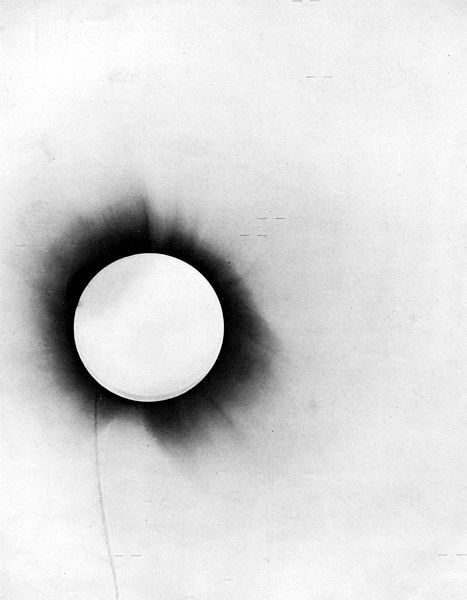
\includegraphics[width=0.8\textwidth]{Intro/1919_eclipse_negative.jpg}
\caption[Photometric plates from the 1919 solar eclipse]{From \citet{Dyson:1920zl}, original caption: ``From the report of Sir Arthur Eddington on the expedition to verify Albert Einstein's prediction of the bending of light around the sun. In Plate 1 is given a half-tone reproduction of one of the negatives taken with the 4-inch lens at Sobral. This shows the position of the stars, and, as far as possible in a reproduction of this kind, the character of the images, as there has been no retouching. A number of photographic prints have been made and applications for these from astronomers, who wish to assure themselves of the quality of the photographs, will be considered as as far as possible acceded to."}
\label{intro:fig:eclipse}
\end{figure}

%===============================================================
%   Extragalactic Gravitational Lensing
%===============================================================

\section{Extragalactic Gravitational Lensing}

Fritz Zwicky and Albert Einstein both suggested that galaxies rather than stars would make for much stronger gravitational lenses \citep{Zwicky:1937yq,Einstein:1936cl}. And indeed, later in the 20th century, astronomers began discovering this deflection of light, or gravitational lensing as it became known, by extragalactic sources. In rare cases, the deflection can be strong enough such that the light from the background source can travel multiple paths around the deflecting, or lensing, object, thus creating multiple images of the background source. In 1979, the ``Twin Quasar" was discovered -- two quasars located unusually close together in the sky, both behind a massive foreground galaxy, shown in Figure~\ref{intro:fig:quasar}. Due to the similar redshifts and spectra of the quasars, it was deduced that they were lensed images of the same background quasar.

\begin{figure}
\centering
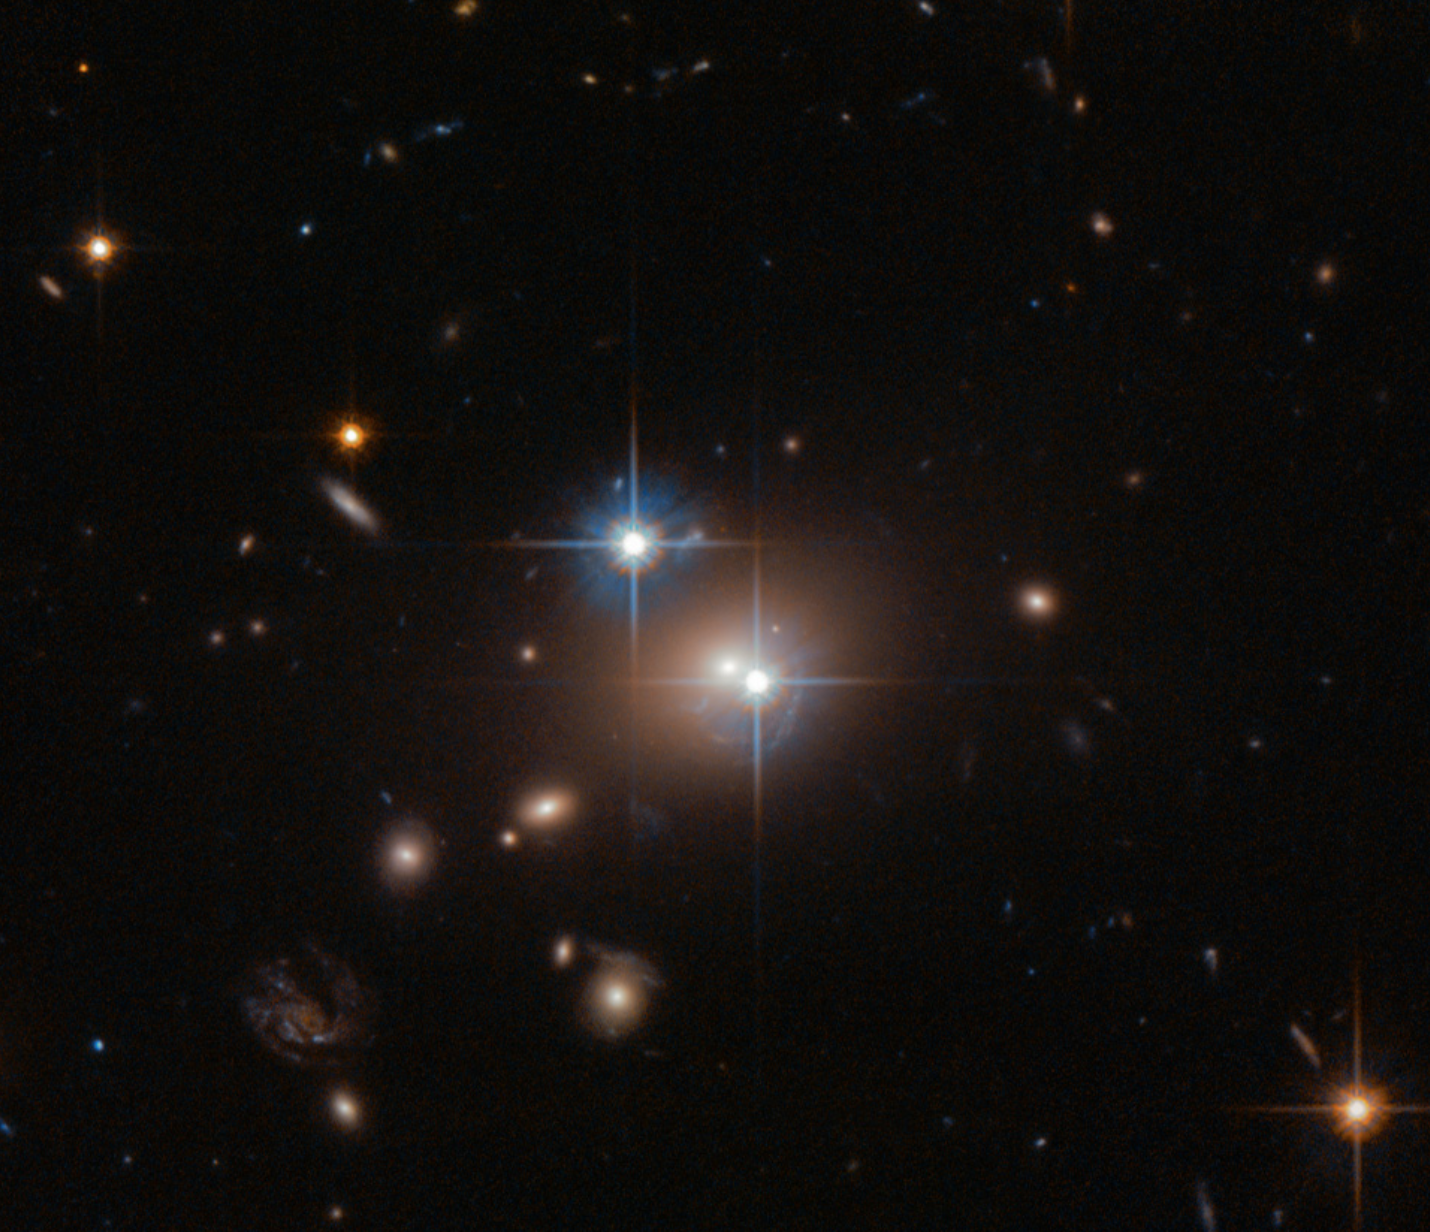
\includegraphics[width=0.8\textwidth]{Intro/twin_quasar.png}
\caption[\hst\ image of the Twin Quasar]{{\it Hubble Space Telescope} (\hst) image of the famous Twin Quasar. From  ``Seeing double". ESA/Hubble Picture of the Week. Retrieved 30 November 2017.}
\label{intro:fig:quasar}
%http://www.spacetelescope.org/images/potw1403a/
\end{figure}

Galaxy clusters are the most massive gravitationally-bound objects in the Universe, consisting of hundreds of galaxies clustered within a virial radius of on the order of a megaparsec. Zwicky used galaxy clusters to hypothesize the existence of an invisible mass in galaxy clusters, as the velocity dispersion of the galaxies suggested the total masses of these clusters to be $400\times$ higher than the mass implied by the star light of the galaxies \citep{Zwicky:1937yq}. This dark matter, as it has come to be known, has been proven time and time over to exist. Only $\sim1\%$ of of the mass of a typical galaxy cluster consists of baryons contained in cluster member galaxies. Nearly $\sim90\%$ of the mass consists of dark matter. The remaining $\sim9\%$ is contained in the 10 million degree intergalactic medium, which would have been ``invisible" to Zwicky, but today is visible with Xray telescopes.

Any galaxy cluster is capable of being a weak lens; however, fewer clusters are capable of behaving as strong lenses.  In order to find these rare strong lenses, the lensed galaxies would need to be highly magnified and distorted significantly as to be seen as obvious signs of lensing. This work would have been impossible on photographic plates as faint lensed galaxies could easily be mistaken for cluster member galaxies or optical defects in the plate. Ultimately, it took the sensitivity and resolution of the CCD camera that allowed for the discovery of gravitational lenses. And indeed, the first spectroscopically-confirmed cluster lensed galaxy was discovered in the field of Abell 370 in 1986 \citep{Soucail:1988kx,Soucail:1987sf,Soucail:1987rz}, shown in Figure~\ref{intro:fig:a370}. Interestingly, we will learn more about this cluster using sophisticated gravitational lens modeling in Chapter~\ref{chap:hff_clusters}.

\begin{figure}
\raisebox{50pt}{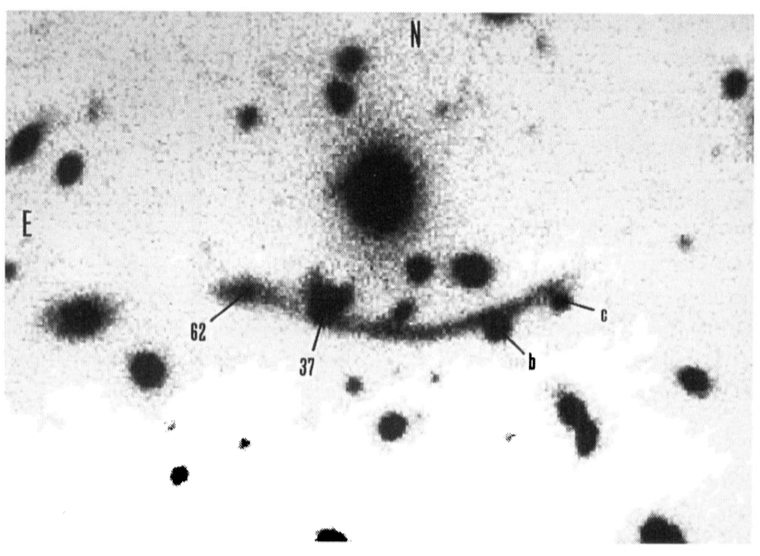
\includegraphics[width=0.35\textwidth, trim=0 10pt 0 0, clip, angle=-28]{Intro/soucail88.png}}
\includegraphics[width=0.55\textwidth, trim=100pt 200pt 100pt 200pt, clip]{Intro/a370_hff.jpg}
\caption[Images of Abell 370 -- the first cluster lens]{Left: From \citet{Soucail:1988kx}, original caption: ``CCD frame of the giant arc in A370. This picture was obtained by J.L.~Prieur at the prime focus of the 3.60m Canada-France-Hawaii telescope on October 25th, 1987. The CCD was a $640\times1024$ RCA2: scale 0.2"/pixel -- seeing 0.7", with an exposure time of 10 minutes in white light. Note the shape of the object \#37, which was already suspected based on its spectrum \citet{Soucail:1987sf}", meaning that since the object is not at the cluster redshift, but indeed behind it and being lensed into a fantastic arc. Right: 140-orbit \hst\ image of Abell 370 from the Hubble Frontier Fields Director's Discretionary Program. From ``The last of the Frontier Fields -- Abell 370. STScI. Retrieved 30 November 2017.}
% https://www.spacetelescope.org/images/heic1711a/
\label{intro:fig:a370}
\end{figure}

%===============================================================
%   Gravitational Lensing Theory
%===============================================================

\section{Gravitational Lensing Theory}

\subsection{The one-dimensional lensing equation}

\begin{figure}
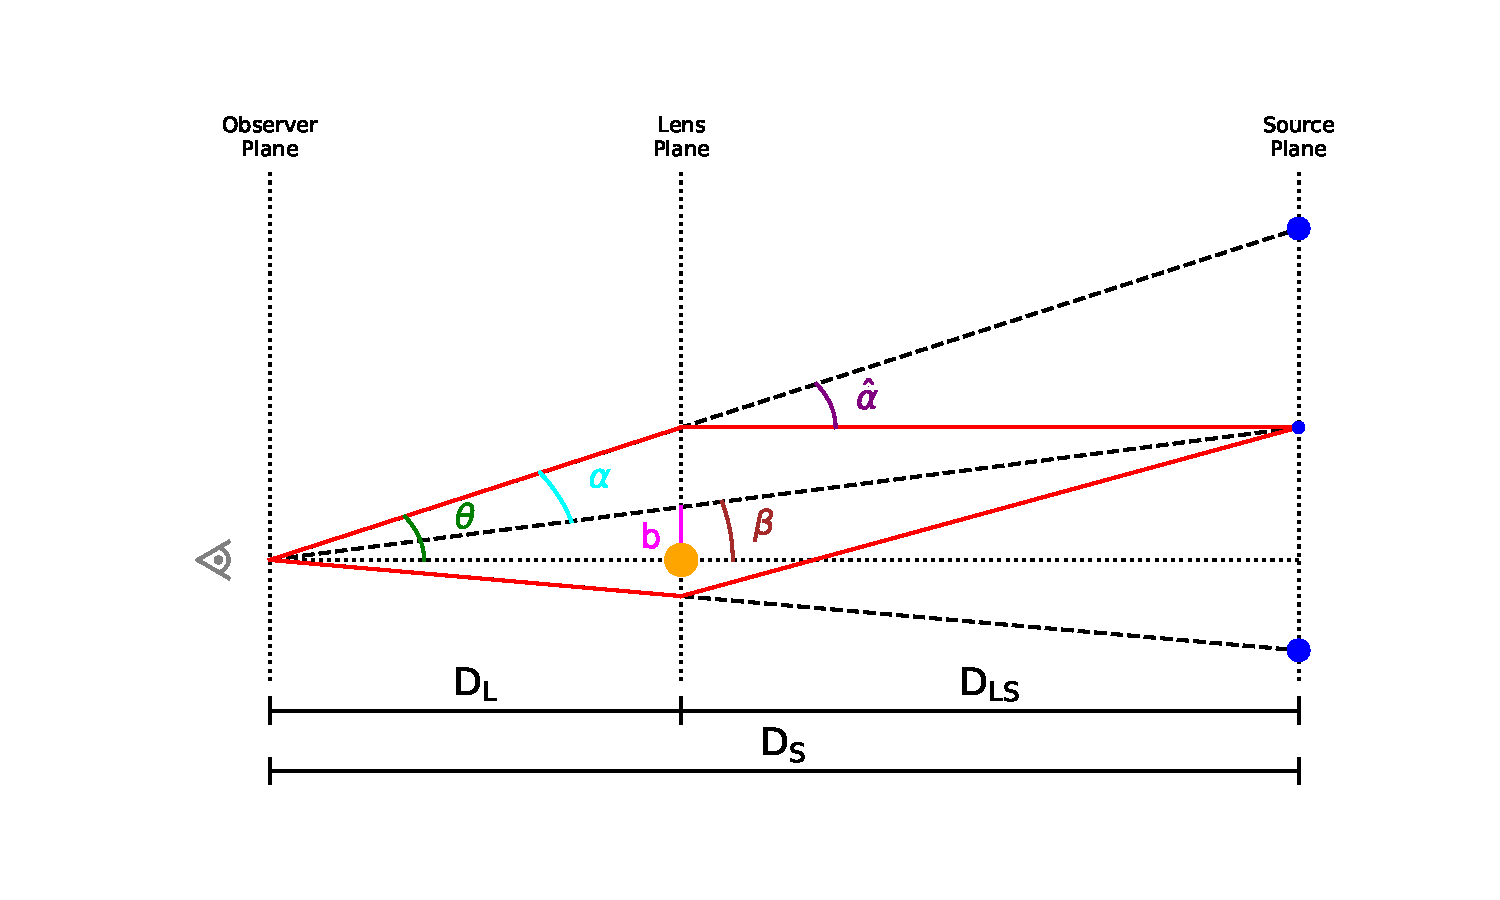
\includegraphics[width=\textwidth, trim=75pt 75pt 75pt 75pt]{Intro/lens_diagram.pdf}
\caption[Diagram of gravitational lensing parameters]{Diagram showing the definitions of angles and distances used for deriving the lens equation.}
\label{intro:fig:diagram}
\end{figure}

Since the distances of between the lens, source, and observer are much larger than the size of the lens itself, it is safe to use the ``thin lens approximation" popular in optics where we assume an instantaneous deflection of the light on a plane of lensing mass. Therefore, we envision the geometry of the lensing as shown in Figure~\ref{intro:fig:diagram}. The distances $\dl$, $\ds$, and $\dls$ are the angular diameter distances between the observer-lens, observer-source, and lens-source, respectively. We define the angle between the lens and source in the observer's frame to be $\beta$ and the angle between the lens and of the apparent position of the image of the source to be $\theta$. The angle $\hat\alpha$ is the deflection angle computed by Einstein in (\ref{intro:eqn:deflection}). Using the small-angle approximation, we can write

\begin{equation}
\theta \ds = \beta \ds + \hat\alpha \dls,
\end{equation}

\noindent and after rearranging, we get that

\begin{equation}
\beta(\theta) = \theta - \frac{\dls}{\ds} \hat\alpha,
\end{equation}

\noindent known as the lensing equation. Here, we have redefined $\beta$ as a function of $\theta$ as every image will map to only a single source, which should be fairly intuitive. We can also define another variable

\begin{equation}
\alpha \equiv  \frac{\dls}{\ds} \hat\alpha,
\label{intro:eqn:dlsds}
\end{equation}

\noindent which is the angular offset between the image and the source at the location of the observer. While $\hat\alpha$ will always remain constant for a given impact parameter, the observed deflection depends on the geometry of the lensing system, i.e., the relative distances to the source and lens.

\subsection{Lensing in two-dimensions and magnification}
\label{intro:sec:magnification}

We have so far been working in one dimension considering positions of sources and images on singular axes. The solutions hold for any axisymmetrical lens; however, in nature, we must consider that mass distributions are more complex, and thus will cause a dependence on position angle of the source rather than purely the impact parameter, $\theta\dl$. In the simple case shown in Figure~\ref{intro:fig:diagram}, our one-dimensional lens has produced two point source images. This is also true if we extend the solution to two-dimensions, except in the instance where source is directly behind the lens ($\beta=0$). In this case, the solution is a circle (or ring) of radius

\begin{equation}
\theta = \alpha = \frac{\dls}{\ds} \frac{4GM}{c^2} \frac{1}{\theta \dl}
\end{equation} 

\noindent from which we define the Einstein radius as

\begin{equation}
\theta_E^2 \equiv \frac{4GM}{c^2} \frac{\dls}{\dl\ds}.
\label{intro:eqn:einstein_radius}
\end{equation}

\subsection{Lens mapping}

Most sources in the Universe are not point sources and can be magnified, in that the solid angle subtended by their images is larger than that of the source. The exact definition of the magnification is the ratio of these solid angles,
$\mu \equiv \Delta \theta/\Delta \beta$. We can also treat lensing as a mathematical transformation of the shape of a source into its observed images. We can rewrite the lens equation as a transformation matrix

\begin{equation}
A_{ij} = \frac{\partial \beta_{ij}}{\partial \theta_{ij}} = \delta_{ij} - \frac{\partial{\alpha_{i}}}{\partial{\theta_{j}}} = 
	\begin{bmatrix}
		1-\kappa-\gamma_1 & \gamma_2 \\
		\gamma_2 & 1-\kappa+\gamma_1
	\end{bmatrix},
\end{equation}

\noindent where we have defined the new terms

\begin{align}
\kappa &= \frac{1}{2} \left(\frac{\partial{\alpha_{1}}}{\partial{\theta_{1}}}+\frac{\partial{\alpha_{2}}}{\partial{\theta_{2}}}\right) = \frac{1}{2} \nabla_{ij} \alpha_{ij} = \frac{\Sigma}{\Sigma_{crit}} \label{intro:eqn:kappa} \\
\gamma_1 &= \frac{1}{2} \left(\frac{\partial{\alpha_{1}}}{\partial{\theta_{1}}}-\frac{\partial{\alpha_{2}}}{\partial{\theta_{2}}}\right) \\
\gamma_2 &= \frac{\partial{\alpha_{1}}}{\partial{\theta_{2}}} = \frac{\partial{\alpha_{2}}}{\partial{\theta_{1}}} \\
\gamma^2 &= \gamma_1^2 + \gamma_2^2
\end{align}

\noindent with $\Sigma$ representing the projected surface mass density of the lens plane, with critical surface mass density equal to

\begin{equation}
\Sigma_\mathrm{crit} = \frac{c^2}{4\pi G} \frac{\ds}{\dls\dl}.
\end{equation}

\noindent The formation of multiple and/or highly distorted images, occurs when $\kappa>1$. We see in (\ref{intro:eqn:kappa}) that lensing depends not only on how massive the lens is ($\Sigma$), but also its proper geometrical alignment with the source ($\Sigma_\mathrm{crit}$).

The magnification map can be determined by taking the inverse determinant of the transformation matrix:

\begin{equation}
\mu^{-1} = |\det A| = |(1-\kappa)^2 - \gamma^2|.
\end{equation}

\noindent It is possible for the magnification to be smaller than one (i.e., demagnified images) as well as become infinite. However, the area in the image plane where this occurs is infinitesimally small, so infinite magnifications fall on lines called critical curves. The eigenvalues of $A$ tell us where these lines occur:

\begin{align}
1-\kappa-\gamma &= 0 \\
1-\kappa+\gamma &= 0.
\end{align}

\noindent These describe the tangential and radial critical curves in the image plane, respectively. These are the lines of symmetry between image pairs, reflected either tangentially or radially. Image pairs will have opposite parity; they are mirror images of one another. We can use the lens equation to map these curves to the source plane, producing caustics that inform us on the number of images the lens will produce. The number of images must always be odd, with two additional images being formed for each caustic the source falls within. Often times one of these images is highly demagnified and/or lies behind the bright galaxy, thus is not always observed and the reason there are reports of ``double" or ``quad" configurations in the literature. Typical image configurations and their respective source locations are shown in Figure~\ref{intro:fig:image_config}.

For the remainder of this work, we will refer to ``strong" gravitational lensing as the phenomenon in which lensing results in multiple and/or highly-distorted images of the background source.

\begin{figure}
\centering
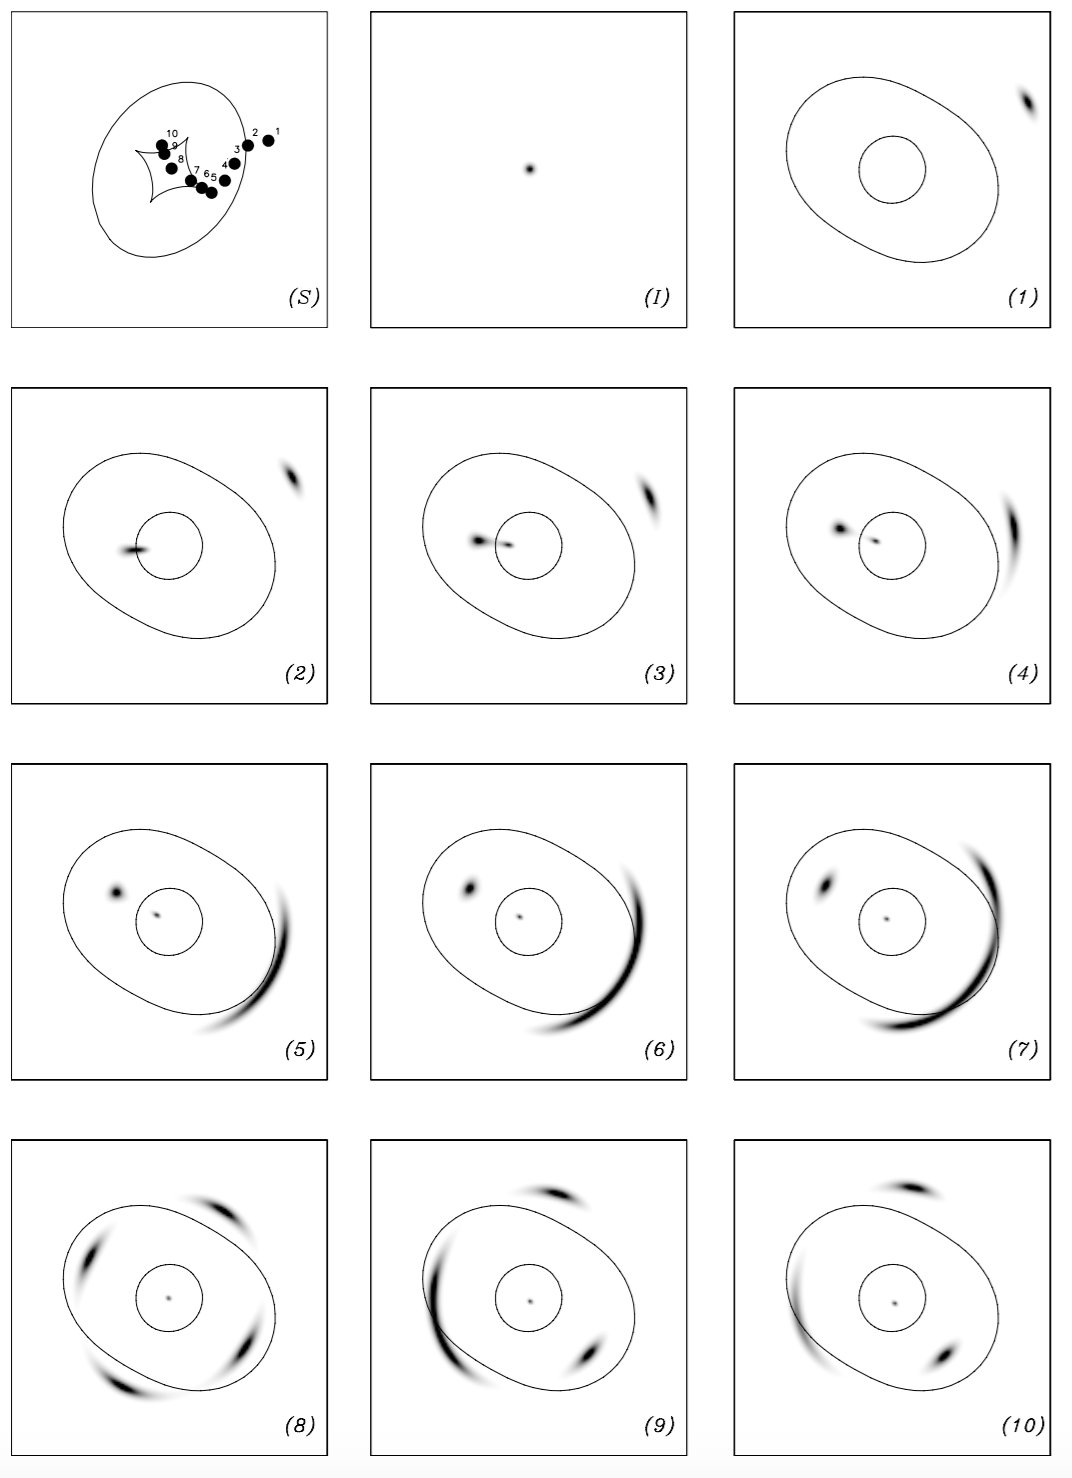
\includegraphics[height=0.8\textheight]{Intro/image_config.png}
\caption[Strong lensing caustics, critical curves, and multiple image configurations]{From \citet{Kneib:2011qy}, original caption: ``Multiple-image configurations produced by a simple elliptical mass distribution. The panel (S) shows the caustic lines in the source plane and the positions numbered 1 to 10 denote the source position relative to the caustic lines. The panel (I) shows the image of the source without lensing. The panels (1) to (10) show the resulting lensed images for the various source positions. Certain configurations are very typical and are named as follows: (3) radial arc, (6) cusp arc, (8) Einstein cross, (10) fold arc."}
\label{intro:fig:image_config}
\end{figure}

\section{Strong gravitational lens modeling}

\subsection{First-order approximation for the mass of the lens: Einstein radius}

As we found in \S~\ref{intro:sec:magnification}, sources which are almost perfectly aligned with the lens will produce an Einstein ring. By assuming that the lens is axisymmetric, we can determine the total mass within this ring from (\ref{intro:eqn:einstein_radius}), which yields

\begin{equation}
M(<\theta_E) = \pi (\theta_E \dl)^2 \Sigma_\mathrm{crit}.
\label{intro:eqn:einstein_mass}
\end{equation}

Figure~\ref{intro:fig:einstein_ring} shows examples of nearly perfect Einstein rings where this approximation can be made. Typical values for $\theta_E$ in clusters are on the order of $\sim$15", translating to physical scales on the order of a few hundred kiloparsecs. All other estimates for masses based on astronomical observables (ex., X-ray, Sunyaev-Zel'dovich effect, galaxy dynamics, weak lensing, galaxy counts, etc.) are sensitive to the masses at much larger radii ($\sim0.5-1.5$ Mpc). Thus, strong lensing provides a unique estimate for the masses at the very cores of clusters. In conjunction with other techniques, strong lensing can be used to measure the mass-concentration relationship of galaxy clusters, which helps inform their formation history.

\begin{figure}
\centering
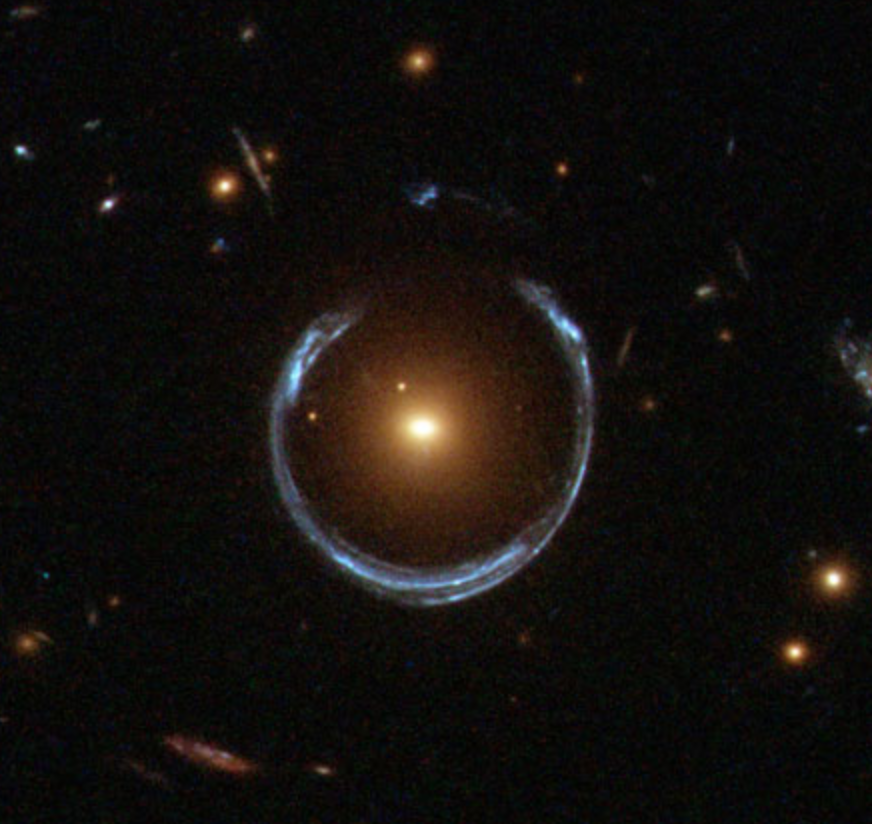
\includegraphics[height=0.3\textheight]{Intro/einstein_ring_1.png}
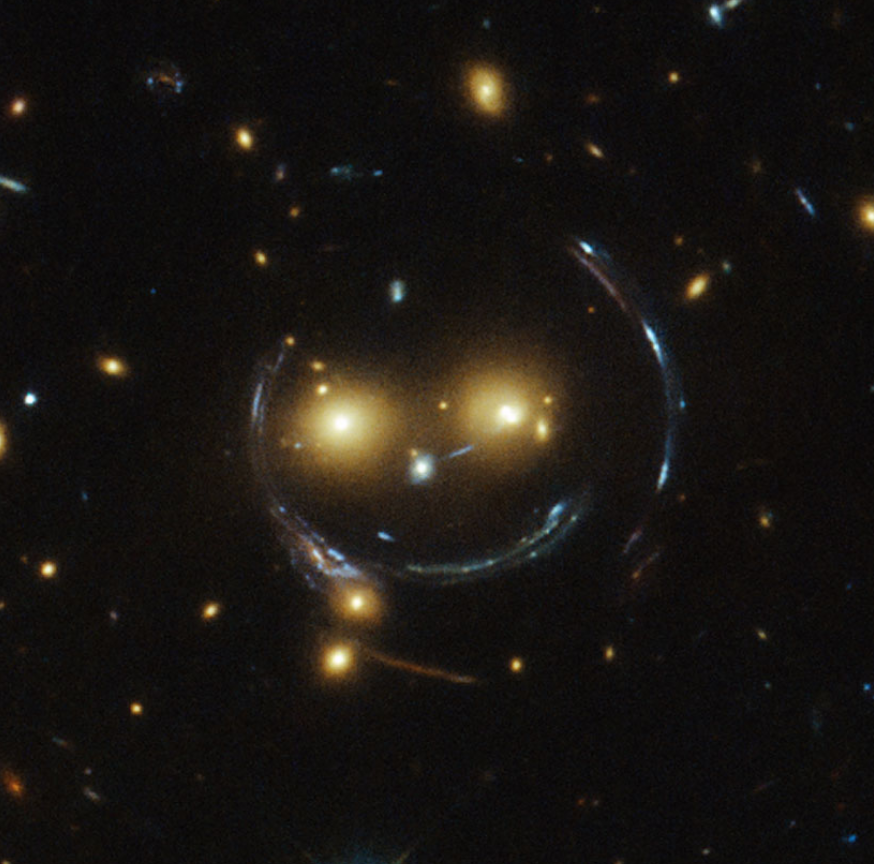
\includegraphics[height=0.3\textheight]{Intro/einstein_ring_2.png}
\caption[\hst\ Einstein Rings]{Two famous Einstein rings imaged with the \hst. (Left): LRG~3-757 nearly forms a perfect ring around the massive elliptical galaxy. (Right): Galaxy cluster SDSS~J1038+4849 forms a pseudo-Einstein ring with partial rings formed from several lensed background sources.}
% http://apod.nasa.gov/apod/ap111221.html
% https://en.wikipedia.org/wiki/Einstein_ring#cite_note-NASA-20150210-6
\label{intro:fig:einstein_ring}
\end{figure}

However, galaxy clusters are not necessarily axisymmetric and contain a lot of substructure and galaxies, which perturb the local lensing potential. While it is a close approximation, a precise determination of the mass distribution requires more careful modeling which can take into account shape and substructure of the cluster.

\subsection{Lens modeling}

A more precise model of the lensing mass can be achieved using the positions of multiple images. By finding a deflection field that maps all multiple images to a single position in the source plane, an estimate for the mass can be computed using (\ref{intro:eqn:kappa}). Using more sets of multiple images will help to further constrain the deflection field at different radii. After examining (\ref{intro:eqn:einstein_mass}), we see that $\Sigma_\mathrm{crit}$ is linear with $\alpha$ and thus scales in the same manner as (\ref{intro:eqn:dlsds}). Having a range of redshifts from different sources will produce a range of Einstein radii, which will help to constrain the slope of the mass distribution (such as the cluster in the right image of Figure~\ref{intro:fig:einstein_ring}).

The general approach to lens modeling involves finding the mass distribution which creates the deflection field that best reproduces the observed image configuration. These approaches fall into two categories: ``parametric" and ``non-parametric". The former involves defining the surface mass density of the cluster and its galaxies in terms of physically-motivated potentials such as an isothermal sphere or a Navarro, Frenk, and White profile \citep[NFW; ][]{Navarro:1997qa}. The cluster dark matter halo is represented by a physically-motivated potential, with cluster member galaxies added as additional perturbers. The methods for assigning mass to cluster member galaxies rely heavily on the assertion that ``light traces mass." Therefore, the total mass of the galaxy is scaled by the total light from the galaxy, usually following the empirical fundamental plane of luminosity, radius, and velocity dispersion of elliptical galaxies \citep{Gudehus:1973kq}. ``Non-parametric" methods allow for more flexible characterization of the mass distribution by employing either a pixelized array of masses or a grid of radial basis functions that can each fluctuate in total mass to affect the localized deflection near multiple images as well as the overall shape of the mass distribution. Generally, this method does not force the notion that galaxies must have mass, but allows for the image configurations to constrain the masses on smaller-scale structures as needed to reproduce the lensing effect.

The modus operandi of this author is a parametric method established by the \texttt{LENSTOOL} software \citep{Jullo:2007lr} and embodies the lens modeling inquiry presented in this dissertation. Therefore, detailed discussions of the variants of non-parametric methods is beyond the scope of this work.

\subsubsection{Bayesian statistics and model optimization}

Regardless of the modeling method, nearly all have settled on exercising a Bayesian approach, where optimizing a model depends not only on its fitness, but also information about the parameters obtained a priori. The Bayes' theorem is defined

\begin{equation}
P(\vec{p} | D ) = \frac{P(\vec{p}) P(D | \vec{p} ) }{P(D)}
\label{intro:eqn:bayes}
\end{equation}

\noindent where $D$ are the observed data, and $\vec{p}$ contains the parameters of the model. Let us break down each component of (\ref{intro:eqn:bayes}):

\begin{itemize}
\item $P(\vec{p} | D )$: The posterior probability distribution -- the probability of the model given the data. In this instance, the data are the locations of the multiple images along with their distance from the lens and observer (i.e., redshift).
\item $P(\vec{p})$: The prior. This term is the a probability that a particular model is accurate based on {\it a priori} information.
\item $P(D | \vec{p} )$:  The likelihood of getting the data given the parameters of the model. Non-Bayesian modeling focuses this term in optimization (i.e., maximum likelihood estimation) and de-regulates the prior.
\item $P(D)$: The evidence. This term is the probability that a particular model is valid independent of all other variables, which effectively acts as Occam's razor: ``All things being equal, the simplest solution tends to be the best one." The evidence normalizes the posterior probability distribution.
\end{itemize}

Bayes' theorem can easily be applied to strong lens modeling once we define a likelihood function to include in our optimization. The likelihood function will take the form

\begin{equation}
P(D | \vec{p} ) = \prod_{i=1}^N \frac{1}{  \prod_{j=1}^{n_i} \sigma_{ij} \sqrt{2\pi} } \exp^{-\frac{\chi_i^2}{2}},
\label{intro:eqn:likelihood}
\end{equation}

\noindent where $N$ is the number of sources, $n_i$ is the number of images of each source $i$, and $\sigma_{ij}$ is the measurement error of image $j$ of source $i$. By minimizing $\chi^2$, we will produce the maximum likelihood model. Our goal in lens modeling is to find a solution with the smallest scatter between the source positions mapped to each of its images. Defining the likelihood in this manner is called source plane optimization. While this still solves the lens equation, it is not ideal as the position of the sources are unknown to the observer. The more appropriate method would be image plane optimization, which involves an extra step of ray tracing the source position of each image back out to the image plane and measuring the scatter of the predicted images. However, this second step is much more computationally intensive due to the ray tracing, which is required because the lens equation is not invertible. The $\chi_i^2$ function for each source $i$ will then take the form

\begin{equation}
\chi^2 = \sum_{j=1}^{n_i} \frac{[\theta_\mathrm{obs}^j - \theta^j (\vec{p})]^2}{\sigma_{ij}^2},
\label{intro:eqn:chi2}
\end{equation}

\noindent where $\theta^j (\vec{p})$ is the predicted image position ray traced to the observed image position $\theta_\mathrm{obs}^j$. Examining this equation further, we can see that image plane optimization will ensure that models which produce additional images than those observed are likely to be rejected as they will produce much higher $\chi^2$ than models with fewer images (smaller $n_i$).

It should be noted that this method could be improved by including additional lensing information in the optimization, such as magnification, time delays, and/or flexion (i.e., shape), which could be added in quadrature to (\ref{intro:eqn:chi2}). Some lens modeling methodologies do include these terms; however, for this work, we will only consider image positions as the primary constraint.

\subsubsection{Computational methods}

The \texttt{LENSTOOL} software utilizes a Markov Chain Monte Carlo (MCMC) to sample parameter space to determine the shape of the posterior probability distribution. In the MCMC burn-in phase, ``walkers" of models are initialized with a set of parameters randomly sampled from the current posterior probability distribution. At the first stage, the likelihood has not been sampled yet, so it is not included in the initial determination of the posterior. This is done by replacing the likelihood in Bayes' theorem (\ref{intro:eqn:bayes}) with the term $P(D | \vec{p} )^\lambda$, where $\lambda$ is a ``cooling" parameter. At the beginning, $\lambda=0$, so in the analogy to thermodynamics, the model selection is ``hot" and samples from a wide range of values in parameter space, ensuring that the MCMC can find a global maximum likelihood. The posterior probability for each walker is computed, and a new $\vec{p}$ is selected for each walker and given a probability to jump based on the ratio of the posterior probability of the current position and the new position. Walkers will tend to jump to higher posterior probabilistic positions in parameter space as the chain continues to form, all while $\lambda$ is slowly increasing from 0 to 1 at a rate chosen to insure a smooth convergence towards a colder posterior probability distribution. After $\lambda=1$, the burn-in phase is complete and the chains are re-initialized from the last position in parameter space for all the walkers. Using the full Bayes' theorem, a new MCMC runs to sample the posterior probability distribution.

\subsection{Data for cluster lensing}

Lens modeling has benefited from the imaging CCDs aboard the {\it Hubble Space Telescope} (\hst). The high sensitivity and high resolution allow for easier detection and identification of multiple image systems to be used in the modeling. The first remarkable instance of using \hst\ for cluster lensing of Abell 2218 \citep{Kneib:1996kb} imaged with the Wide Field Planetary Camera 2 (WFPC2) is shown in Figure~\ref{intro:fig:lensing_clusters} (with more recent imaging added). 

\begin{figure}
\centering
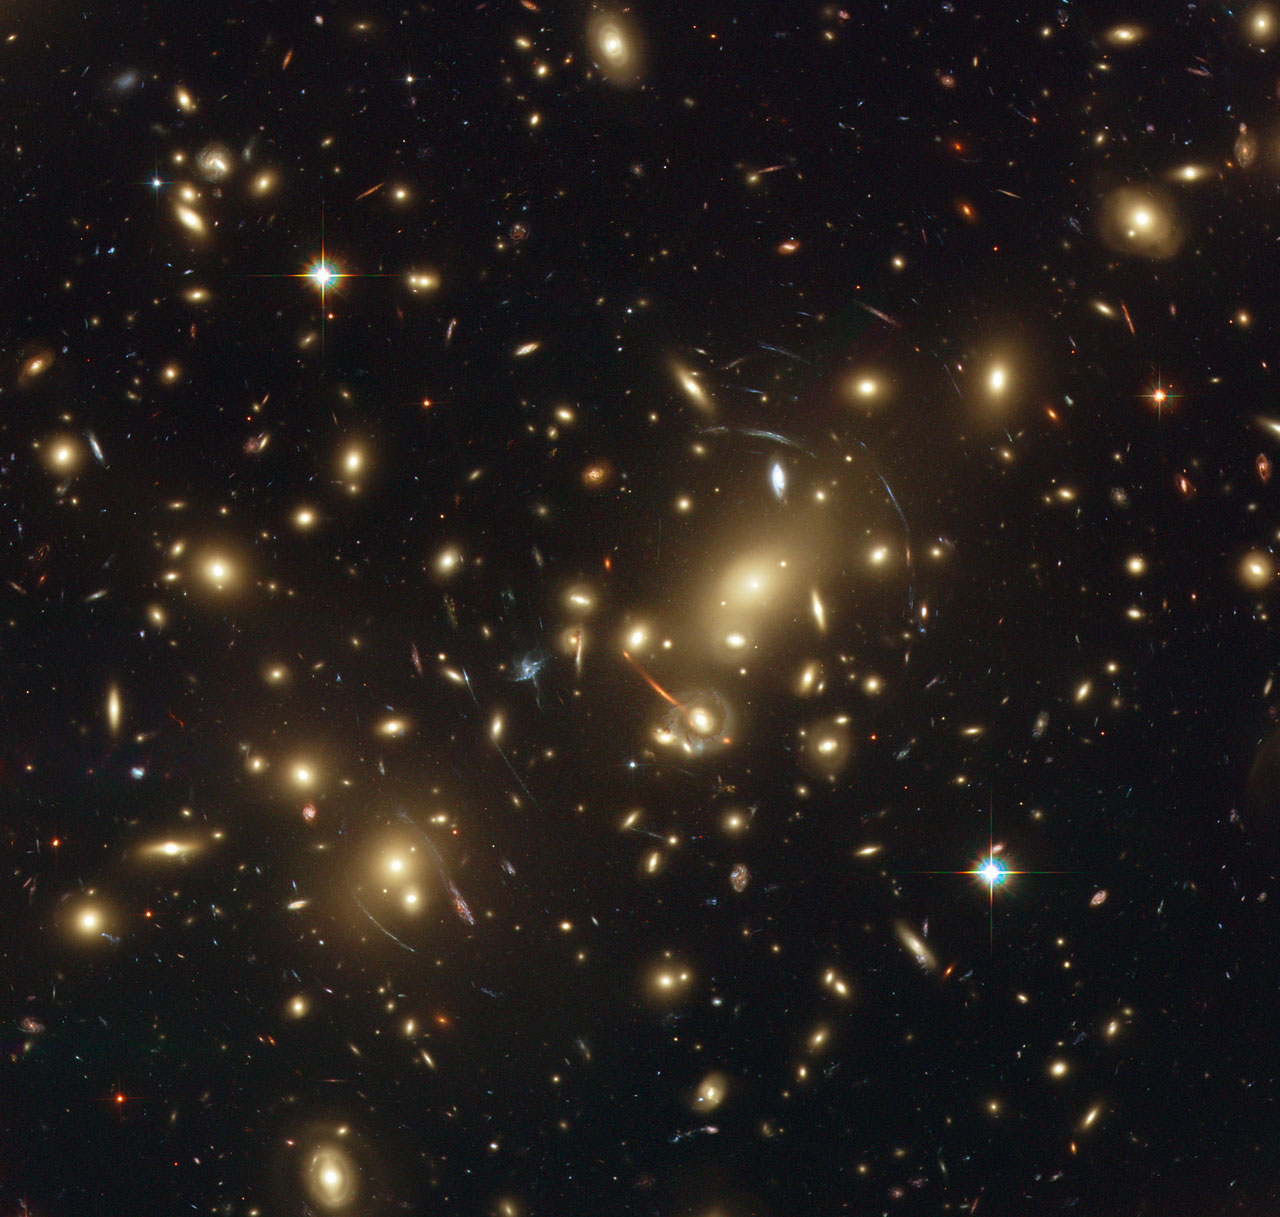
\includegraphics[height=0.3\textheight]{Intro/a2218.jpg}
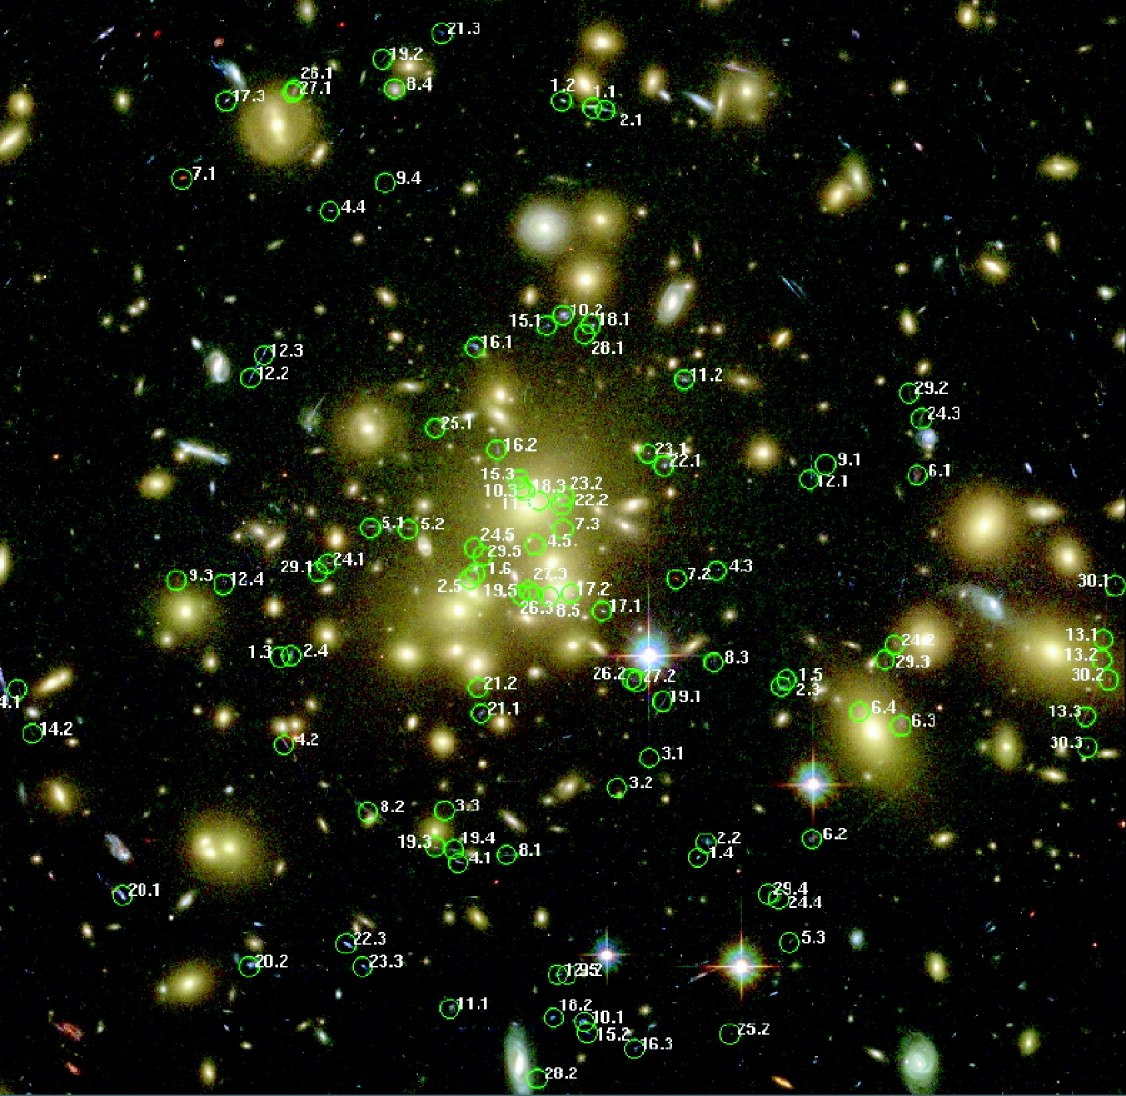
\includegraphics[height=0.3\textheight]{Intro/a1689.jpg}
\caption[Abell 2218 and Abell 1689]{\hst\ imaging of Abell~2218 (left) and Abell~1689 (right).}
\label{intro:fig:lensing_clusters}
\end{figure}

The servicing mission for \hst\ in 2002 gave us the new Advanced Camera for Surveys (ACS), which greatly enhanced optical imaging capabilities. \citet{Broadhurst:2005qy} and \citet{Halkola:2006ss} were able to map the mass distribution in fine detail using over a hundred multiple images of background sources of Abell 1689 with the new ACS data, shown in Figure~\ref{intro:fig:lensing_clusters}. Furthermore, the Wide Field Camera 3 (WFC3) installed during the final servicing mission in 2009 ignited the field of cluster strong lensing with several groups working to develop new lens modeling techniques. This camera has both ultraviolet, optical, and near-infrared imaging sensitivity, allowing for full bandwidth coverage of lensing clusters.

The {\it Spitzer Space Telescope} has also greatly added in the field of cluster lensing. While it cannot achieve the same resolution as \hst, it can greatly help distinguish between foreground and background objects in the field of view with adding data to galaxies' spectral energy distribution (SED) in the far-infrared.

\section{Fantastic lenses and where to find them}

The selection techniques for galaxy clusters exhibiting strong gravitational lensing can generally be split into two categories: ``high mass" and ``high magnification." Galaxy clusters may be selected by mass for lensing, as those more massive will tend to provide a larger cosmological volume for which $\kappa>1$, thus having high cross sections for lensing many background galaxies. However, galaxies need not be massive to lens a single galaxy to a very high magnification ($\mu>30$). The techniques for finding these clusters are different as are their scientific applications.

\subsection{Surveys for finding clusters}

Some of the first galaxy clusters were identified in wide-field optical surveys. For example, the Abell clusters \citep{Abell:1958mz,Zwicky:1968rm,Abell:1989ly} were found in large surveys of photographic plates and identified based on the clustering of several massive red galaxies located within a few arcminutes of one another. Generally speaking, more massive clusters tend to have higher galaxy membership, or ``richness." Abell 1689 and Abell 370, as we discussed earlier, are prime examples. With digitized data, clusters can be found in optical/near-infrared surveys using algorithms aimed at identifying clusterings of galaxies close in photometric redshift estimations \citep{Rykoff:2014rz} and by identifying the red sequence of early-type galaxies on a color-magnitude diagram \citep{Gladders:2000kq}.

With the advent of Xray telescopes, more massive clusters were able to be identified. A hot ionized intercluster medium fills the space between galaxies. In order for this gas to maintain hydrostatic equilibrium within the gravitational potential of the cluster, it must be at a temperature of order $10^7$ to $10^8$ K, with $M\propto T_X^{3/2}$ based on theoretical arguments for a relaxed system \citep{Horner:1999rz}. Plasmas at this temperature will emit high energy photons on the order of a few keV via thermal bremsstrahlung radiation. Massive clusters ($T>5$ keV) can be targeted and identified as lensing clusters with optical imaging. The Massive Cluster Survey \citep[MACS; ][]{Ebeling:2001rt} carried out this method by applying Xray brightness and hardness cuts to sources in the ROSAT All Sky Survey and cross-matched with optical surveys and follow-up observations to find the most massive galaxy clusters at $z>0.3$. The selection effect for Xray-selected clusters is redshift-dependent as a result of cosmological dimming of the emission.

The hot intercluster medium also provides a second means for detection. Photons from the cosmic microwave background (CMB) are cooler than the gas surrounding galaxy clusters and can receive an energy boost from inverse Compton scattering. This phenomenon is known as the Sunyaev-Zel'dovich effect \citep{Sunyaev:1972lr}. As a result, the CMB photons passing through a galaxy cluster will ``disappear" at the frequencies below the thermal null frequency of the CMB at $\sim220$~GHz and ``reappear" at higher frequencies. Over a thousand clusters have been found in the Planck all-sky survey of the CMB \citep{Planck-Collaboration:2014gf}. More massive clusters will have a stronger CMB detriment and there is no cosmological dimming of the signal, thus the sample is mass-limited. However, the large seven arcminute beam can cause significant beam-dilution for sources with angular sizes smaller than the beam, and therefore also takes a hit at detecting clusters at higher redshifts. Other surveys work with smaller beam sizes and thus, while still mass-limited, are able to push cluster detections out past $z=1$. The most massive galaxy cluster beyond $z=0.87$, nicknamed ``El Gordo" \citep{Menanteau:2012ul, Menanteau:2010fu}, was found along with nearly 100 other clusters by the Atacama Cosmology Telescope \citep[ACT; ][]{Hasselfield:2013pd,Marriage:2011qf}. The South Pole telescope \citep[SPT; ][]{Bleem:2015gf} has detected nearly 900 clusters over a 2500 square degrees. 

\begin{figure}
\centering
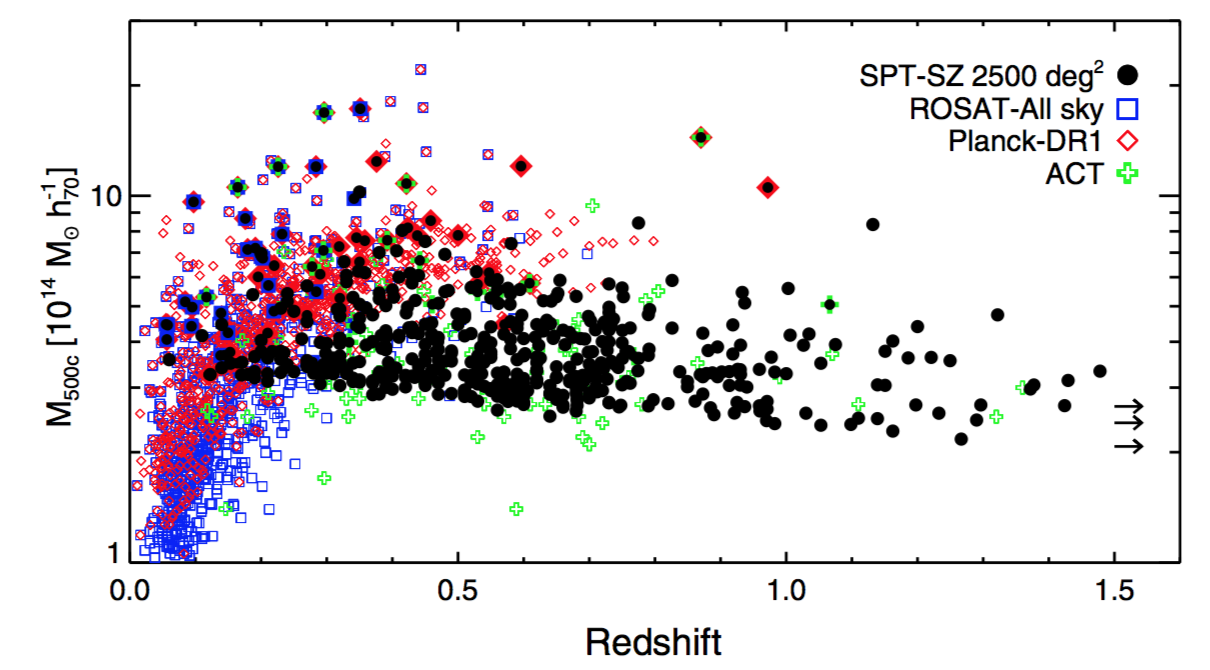
\includegraphics[width=\textwidth]{Intro/spt.png}
\caption[Masses and redshifts of cluster detections]{From \citet{Bleem:2015gf}: The masses and redshifts of optically-confirmed clusters discovered in the SPT, ACT, Planck and ROSAT surveys.}
\label{intro:fig:cluster_detections}
\end{figure}

Figure~\ref{intro:fig:cluster_detections} shows these clusters plotted in mass and redshift. It is important to note that mass is not a direct quantity that any of the methods above can measure. Our best way of measuring the total mass of a galaxy cluster is through weak gravitational lensing, where the integrated surface mass density along the line of sight is measured using the slight distortions in the shapes of background galaxies to map the shear. Since galaxies can intrinsically have elongated shapes, thousands of background sources are needed in order to determine a statistically significant measurement for the shear across the entire field of the cluster. Therefore, high-resolution ($<$1"), wide-field (several square degrees) imaging is needed for these measures, as well as accurate estimates for the redshifts of the background sources, in order to eliminate the mass sheet degeneracy \citep{Schneider:1995vn}. The ``Weighing the Giants" project has measured weak lensing mass and systematics for 51 massive clusters based on imaging from both the {\it Subaru} and {\it Canada-France-Hawaii Telescopes} \citep{von-der-Linden:2014wd}, which can be compared with other scaling relations for mass.

\subsection{Discovering galaxies at cosmic dawn}

``High mass" clusters are the best for finding the most distant galaxies in the Universe. These techniques combine two powerful tools: massive lensing clusters and \hst\ along with deep integrations on the scales of hundreds of orbits. Using lensing can be powerful but makes analysis of determining a luminosity function more difficult. Lensing magnifies not only the sources, but the cosmological volume for which galaxies can be significantly magnified. Because of the smaller survey volume, the counts of lower redshift galaxies in lensed fields can be slightly lower than in unlensed fields, like those of Cosmic Assembly Near-infrared Deep Extragalactic Legacy Survey \citep[CANDELS; ][]{Grogin:2011ly} and the Hubble Ultra Deep Field \citep{Beckwith:2006rt}. However, the cosmological volume containing high magnifications is larger for higher redshifts, so we will see a boost in counts of galaxies at $z>8$. Our best hopes at finding sources with double digit redshifts rely on cluster lensing.

The Cluster Lensing and Supernova Search with {\it Hubble} \citep[CLASH; ][]{Postman:2012lr} used this technique on 20 Xray-selected galaxy clusters and 5 known lensing clusters to be imaged in 16 bands of \hst\ ACS and WFC3. The high photometric resolution allows for more accurate lens modeling, both strong and weak, as well as more accurate photometric redshifts obtained from the well constrained spectral energy distributions of the galaxies from the photometry \citep{Jouvel:2014qy}. CLASH provided the means to set more stringent limits on the star formation rate density at $z=9-10$ \citep{Bouwens:2014zp} as well as precise measurements of the mass-concentration relationships of the lensing clusters themselves \citep{Merten:2015rz,Meneghetti:2014ys}. Several exciting discoveries were also made: a triply-imaged $z\sim11$ candidate was found lensed by cluster MACSJ0647.7+7015 at $z = 0.591$ \citep{Coe:2013tg}, a spectroscopically confirmed, quintuply-imaged $z=6.11$ galaxy was found lensed by Abell S1063 \citep{Monna:2014lr,Balestra:2013uq}, and three lensed supernovae at $z=0.85,1.14,1.28$ were discovered \citep{Patel:2014kl}, two of which were Type Ia and could be used to challenge the magnification predictions of the lens models.

In 2013, a director's discretionary time (DDT) was approved for \hst\ over the course of Cycles 22-24 to image 6 massive clusters, 140 orbits each and in 7 ACS and WFC3/IR bands. This survey, the Frontier Fields \citep{Lotz:2017gd} aimed at pushing beyond the limits of CLASH and predicted to yield up to 70 $z>9$ candidates \citep{Coe:2015qf}. As this was a DDT program, the data are publicly available immediately when downloaded from the telescope, and after a short while, high level data reductions provided by the Space Telescope Science Institute (STScI). Therefore, in efforts to level the playing field for the high redshift community with or without lensing experience, the lens models were also made publicly available (a discussion on this process and the creation of the models is given in Chapter~\ref{chap:hff_clusters} of this dissertation).

\subsection{High-resolution galaxies at cosmic noon}

Finding galaxies lensed to extraordinary magnifications is extremely rare; however, it is possible to find them buried in data sets cataloging thousands of clusters. Scanning through thousands of cut out images of galaxy clusters in optical surveys for the signatures of strong lensing can be a painstakingly tedious process for any individual to endure. But, believe it or not, a lot of dedicated astronomers have carried out this task on data. These projects include the Red Sequence Cluster Survey \citep[RCS;][]{Gladders:2003zr}, the Sloan Giant Arc Survey \citep[SGAS; Gladders~et~al. in preparation, ][see Figure~\ref{intro:fig:gallery}]{Hennawi:2008mz}, SPT optical follow-up \citep{Bleem:2015gf}, and the Dark Energy Survey \citep[DES; ][]{Diehl:2017zh}. Ways of making these tasks less daunting include taking advantage of public interest using citizen science projects like Space~Warps\footnote{https://spacewarps.org/} and by utilizing deep learning algorithms to search large datasets for the signatures of strong lensing \citep{Lanusse:2018zv,Nord:2016kc}.

\begin{figure}
\centering
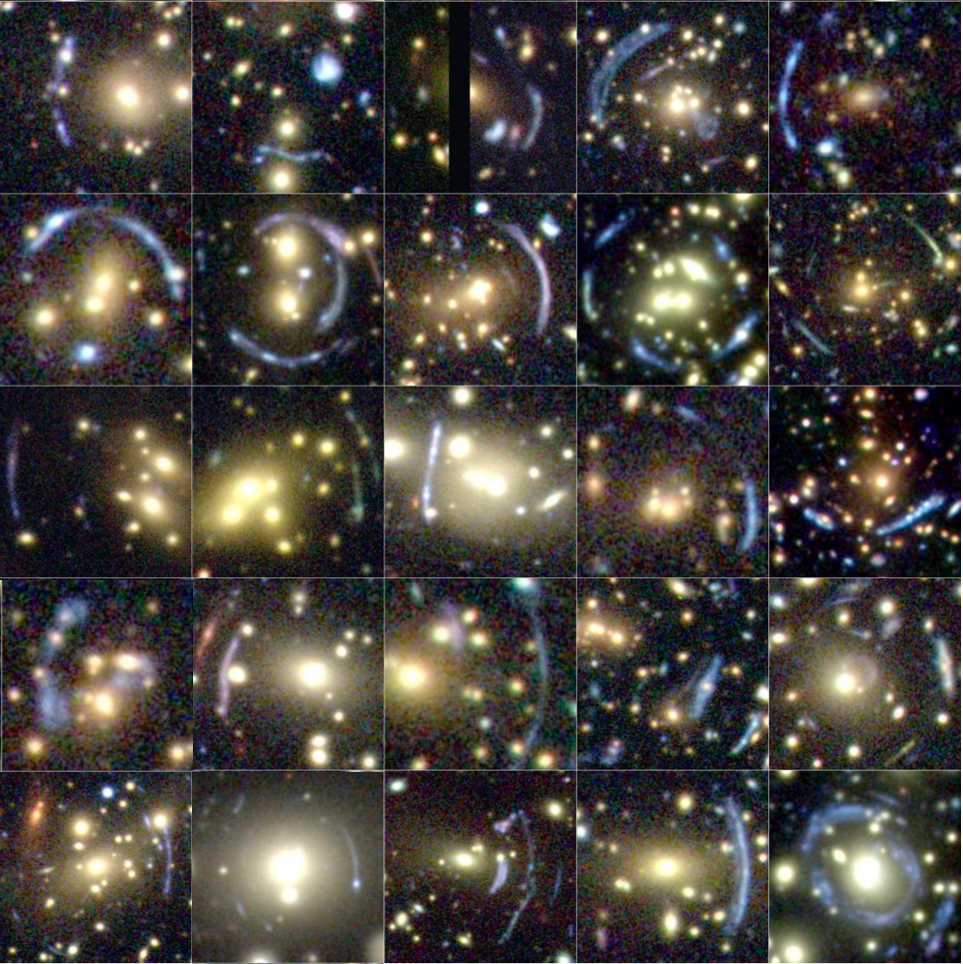
\includegraphics[width=0.8\textwidth]{Intro/gallery.png}
\caption[Gallery of lensing galaxy clusters discovered in SGAS]{A selection of the best lensing clusters found in the Sloan Giant Arc Survey. Each image is $gri$ 5 min exposures with {\it Gemini}/GMOS. Image credit: M.~Bayliss.}
\label{intro:fig:gallery}
\end{figure}

As difficult as it can be to find strong lensing clusters, it is worth it. While it could take weeks to visually inspect a dataset for strong lenses, this effort provides us with data necessary to do high resolution galaxy morphology studies at $z\sim2$ that will be capable on field galaxies not for several years or decades. Lensing amplifies the sizes of galaxies in the sky by factor of roughly the square root of the magnification, allowing us to peer into the fine details of a galaxy, even with only a few orbits of \hst\ data. Chapters~\ref{chap:s1110}-\ref{chap:clumps} of this dissertation show an example of how lensing can allow us to break the kiloparsec resolution limit for galaxies at $z\sim2$. 

As we will discuss in the next section, determining an accurate magnification can be difficult and imparts systematic errors into several derived quantities. However, in most cases, any quantities derived from colors are unbiased because lensing is color-independent. Therefore, lensed galaxies are great laboratories for spectroscopic studies, as observing a single giant arc achieves the same signal-to-noise ratio as a field galaxy in 1/1000th of the exposure time. This allows for a case-by-case study of high redshift galaxies \citep[e.g., ][]{Rigby:2018hs,Rigby:2017yb} rather than relying on stacked spectra from thousands of galaxies \citep[e.g., ][]{Shapley:2003fk}.

\section{Systematics of strong lens modeling}

Strong lens modeling of galaxy clusters has come a long way from where it began over a decade ago. The earliest models often did not provide any statistical errors as doing so at the time would be extremely computationally intensive. Computing power has greatly increased and nearly all lens modeling codes now implement some version of a Bayesian MCMC to adequately sample the parameter space of a lens model from which calculating statistical errors is trivial.

The Frontier Fields lens models were a great experiment for the lens modeling community in the context of beginning to understand systematics. Several teams constructed models with their own techniques using the same lensing information and their models did not produce the same results. Figure~\ref{intro:fig:hff_models} show the differences in the regions of high magnification for the cluster Abell 2744. These modeling variations were of concern as the systematic errors in magnification across the field of the cluster translate directly to systematics in the derived luminosity functions: both in the corrections for intrinsic source luminosity as well as for the size of the survey volume. This prompted the Frontier Fields lens modeling comparison project \citep{Meneghetti:2016xe}, where several lens modeling softwares were put to the challenge of modeling two simulated clusters synthetically ``observed" through the eyes of \hst\ to the same depths as the Frontier Fields. The models produced reliable mass models of the clusters, likely as a result of the many multiple images and constraints provided with full knowledge of the source redshifts. This test was reassuring as the Frontier Fields lens models, with full depth data and several spectroscopic campaigns, are less vulnerable to systematics.

\begin{figure}
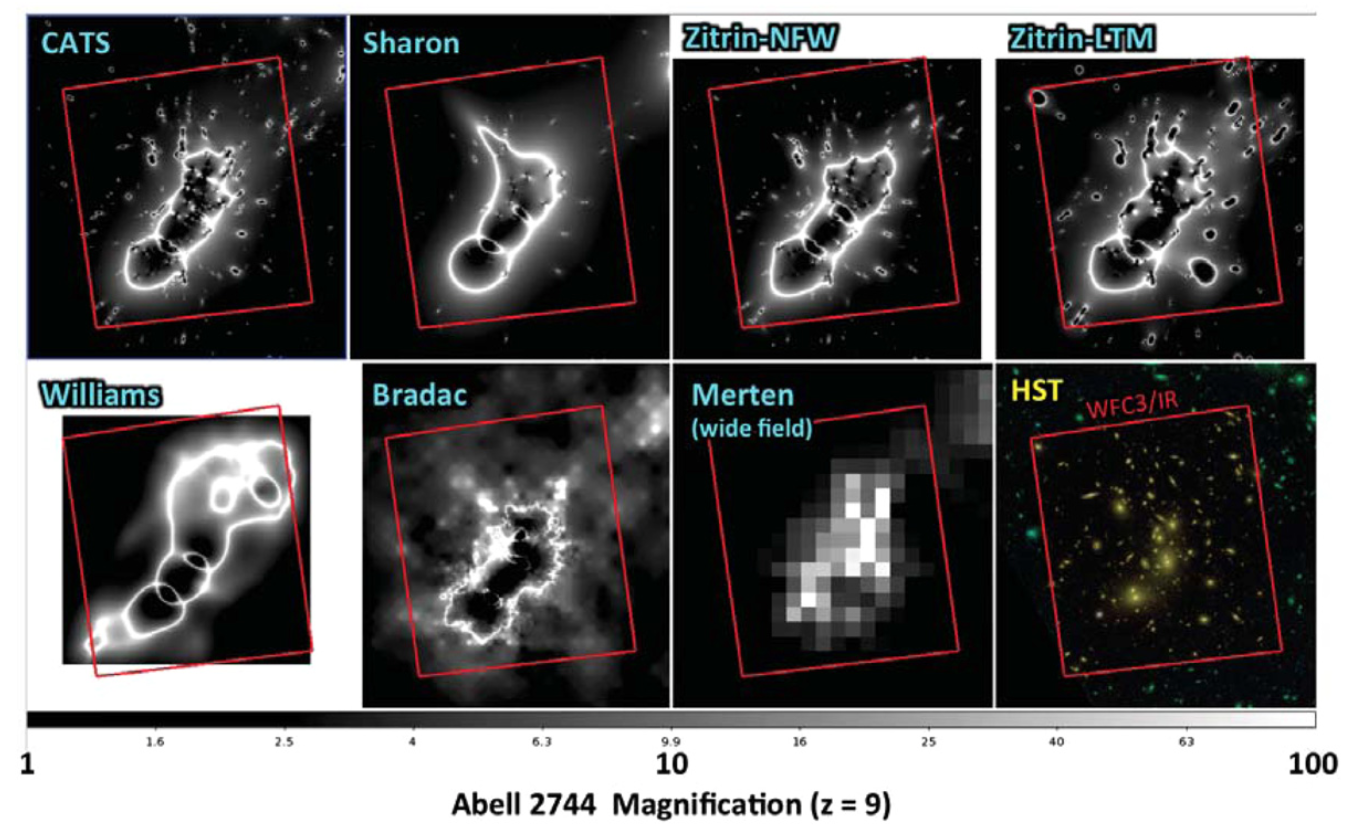
\includegraphics[width=\textwidth]{Intro/hff_models.png}
\caption[Magnification maps of Abell~2744 produced by Frontier Fields lens modeling teams]{From \citet{Coe:2015qf}, original caption: ``Magnification maps (log grayscale) for $z=9$ galaxies lensed by A2744 according to all seven submitted gravitational lensing models. The Frontier Fields WFC3/IR FOV (136"$\times$123") is outlined in red. At bottom right is a color HST image \citep[produced with Trilogy; ][]{Coe:2012px} showing the Frontier Fields WFC3/IR observations (red channel) within the prior ACS observations (blue-green). North is up and East is to the left."}
\label{intro:fig:hff_models}
\end{figure}

It is clear, though, that there was significant systematic error in the lens models of the Frontier Fields produced prior to when the data were taken. These models were built with far few constraints and many only had a few spectroscopic redshifts of the background galaxies. Therefore, a major source of the systematics is in the selection of constraints themselves. The systematic errors in mass and magnification for a cluster like those of the Frontier Fields benefit from increased numbers of constraints and redshifts. However, there is a point where the global systematic errors begin to saturate and are likely a product of the positions and redshift distributions of the constraints themselves. Areas in the image plane where constraints are nearby will have lower statistical and systematic errors, especially if the redshift of that source galaxy is known. This will be discussed further in Chapter~\ref{chap:ares_systematics} and Chapter~\ref{chap:sim}.

\section{Dissertation overview}

This dissertation consists of five chapters demonstrating the use of strong gravitational lens modeling to study the intermediate and high redshift universe, as well as how to better understand and improve our methods when it comes to systematic errors.

Chapter~\ref{chap:hff_clusters} describes the lens models of the six Frontier Fields clusters. These models were created in 2014 using on archival \hst\ imaging supplemented by ground-based spectroscopic observations, including some provided within this chapter. The Frontier Fields lens models created by this author are in addition to several others created using various other lens modeling techniques, all of which are publicly available to the users of the Frontier Fields data sets.

Chapter~\ref{chap:ares_systematics} begins to quantify the systematics involved in this author's lens modeling techniques based on constraint selection and redshift information. Hundreds of lens models of the simulated cluster Ares were realized using different numbers of images and varying levels of precision for the redshift information of the sources. Therefore, we were able to quantify the dependency of errors on mass, magnification, and image plane scatter as they relate to the availability of constraints.

Chapter~\ref{chap:s1110} provides a full lensing analysis of the cluster \cluster. It begins with a description of the hybrid lens modeling technique used to model the mass of the cluster. Then, a forward modeling technique is described and implemented on the giant arc \giantarc\ to create a source plane reconstruction of the source galaxy.

Chapter~\ref{chap:clumps} builds on the previous chapter's source plane reconstruction to report both the sizes and star formation rates of the clumps within the galaxy. These clumps are then compared to the literature, showing an unprecedented level of resolution compared to field galaxies and other source plane reconstructions of lensed galaxies using different methods.

Chapter~\ref{chap:sim} looks briefly at quantifying the systematic errors in a simulated galaxy cluster not all that different from \cluster, where there are very few constraints and spectroscopic redshifts. We will investigate how the effects of adding more spectroscopic redshifts changes the systematic errors in both mass and magnification.

Chapter~\ref{chap:future} provides insight into the future directions of lens modeling in ``the era of precision lensing", where our lens modeling techniques are sophisticated and we have now the computational power to compute the statistical errors on quantities on the levels of a few percent. Fully quantifying systematic errors in the realm of clusters with few constraints and redshifts will be vital in the era of large surveys to come.








\chapter{Lens models and magnification maps of the six Hubble Frontier Fields clusters}
\label{chap:hff_clusters}
\section{Preface}

This work has been adapted by from a paper of the same title in the Astrophysical Journal, Volume 797, page 48 \citep{Johnson:2014tg}, with co-authors Keren Sharon, Matthew B. Bayliss, Michael D. Gladders, Dan Coe, and Harald Ebeling. The paper is adapted and partially reproduced here under the non-exclusive rights of republication granted by the American Astronomical Society to the paper authors.

For this project, I modeled each of the six Frontier Fields clusters using a set of images which were identified by other lens modelers involved in the project. I also designed the Abell S1063 mask and personally took the data at Magellan. I reduced all spectroscopy and (with much help from Michael Gladders) determined the redshifts of the arcs in both Abell 2744 and Abell S1063. I produced all the figures with the exception of Figure~\ref{chap2:fig:volumes} and wrote the vast majority of the text. I produced all of the products publicly-available to the lens community and wrote the first version README file.

%==================================================================================
%   ABSTRACT
%==================================================================================
\section{Abstract}

We present strong-lensing models, as well as mass and magnification maps, for the cores of the six \hst\ Frontier Fields galaxy clusters. Our parametric lens models are constrained by the locations and redshifts of multiple image systems of lensed background galaxies. We use a combination of photometric redshifts and spectroscopic redshifts of the lensed background sources obtained by us (for Abell 2744 and Abell S1063), collected from the literature, or kindly provided by the lensing community. Using our results, we (1) compare the derived mass distribution of each cluster to its light distribution, (2) quantify the cumulative magnification power of the HFF clusters, (3) describe how our models can be used to estimate the magnification and image multiplicity of lensed background sources at all redshifts and at any position within the cluster cores, and (4) discuss systematic effects and caveats resulting from our modeling methods. We specifically investigate the effect of the use of spectroscopic and photometric redshift constraints on the uncertainties of the resulting models. We find that the photometric redshift estimates of lensed galaxies are generally in excellent agreement with spectroscopic redshifts, where available. However, the flexibility associated with relaxed redshift priors may cause the complexity of large-scale structure that is needed to account for the lensing signal to be underestimated. Our findings thus underline the importance of spectroscopic arc redshifts, or tight photometric redshift constraints, for high precision lens models.

All products from our best-fit lens models (magnification, convergence, shear, deflection field) and model simulations for estimating errors are made available via the Mikulski Archive for Space Telescopes. 

%==================================================================================
%   INTRODUCTION
%==================================================================================
\section{Introduction}

Our knowledge of galaxy formation, galaxy evolution, and universal star formation history from shortly after the Big Bang to the present era has greatly increased through deep imaging surveys with the \emph{Hubble Space Telescope} (\hst). These surveys include the Hubble Deep Field \citep{Williams:1996vn}, its successive iterations \citep{Beckwith:2006rt, Bouwens:2011ys, Ellis:2013fr, Illingworth:2013yq}, and the Cosmic Assembly Near-IR Deep Extragalactic Legacy Survey \citep[CANDELS;][]{Grogin:2011ly,Koekemoer:2011fk}. One of the ``final frontiers" for the \hst\ is the detection of the first galaxies to have formed after the Big Bang at $z>8$, the factories that formed the first stars responsible for reionizing the universe \citep{Finkelstein:2012bh}. These deep field surveys have so far discovered a handful of the \emph{brightest} galaxies at these redshifts \citep{Ellis:2013fr,Oesch:2013lq}. Nevertheless, even with the exquisite resolution and depth of \hst, current studies are reaching the limit for finding the \emph{typical} luminosity galaxy at these redshifts; their detectability is affected by cosmic dimming of surface brightness, and most of the redshifted spectral energy distribution we can detect falls in the reddest photometric bands of optical and infrared telescopes. By combining the power of \hst\ resolution with the magnification boost from gravitational lensing, we can overcome some of those observational barriers and attempt to reach survey depths comparable to those of the \emph{James Webb Space Telescope} and 30-meter telescopes, several years before they come online.

Using director's discretionary time as part of the Hubble Deep Field Initiative, the \hst\ Frontier Fields program (HFF; PI: J. Lotz, \hst\ PID 13498) will image four (and up to six) strong lensing galaxy clusters and nearby parallel fields and use them as cosmic telescopes to observe the high redshift universe. Over the next three years, each of these clusters will be imaged in seven photometric bands with ACS and WFC3/IR for a total of 140 orbits per cluster, achieving a depth of 28-29 magnitudes across all bands, much deeper than any cluster observed by \hst\ to date. Typical lensing magnifications for background galaxies in these fields may be $\mu\sim\times2-5$, which increases the depth by an additional $2.5\log_{10}\mu\simeq0.8-1.7$ magnitudes. Therefore, much of the fields can exceed an equivalent depth of 30 magnitudes with the aid of lensing. The HFF will uncover the faint end of the luminosity function at $z\sim8$ and detect the most distant galaxies at $z>10$, the primordial predecessors to today's $L^\star$ galaxies.

The added magnification factor from the lensing clusters can influence the derived physical properties of galaxies (i.e., source luminosity, size, stellar mass, star formation rate) and can thus have an effect on the number counts and resulting luminosity functions.\footnote{For more information, see the gravitational lensing primer for HFF users (http://archive.stsci.edu/prepds/frontier/lensmodels/webtool/ hlsp\_frontier\_model\_lensing\_primer.pdf).} Proper analysis of the galaxies in these fields will require a deep understanding of the intervening lensing system, thus adding a layer of complexity compared to the analysis of ``blank" (i.e., not lensed) fields. To enable the analysis of the lensed sources as soon as the HFF observations become available, five independent teams were chosen to create preliminary lens models (this work included) for each cluster based on existing archival \hst\ imaging and ground-based data. These models of the lensing potential, derived from a variety of lens modeling techniques, are publicly available to the community and can be used to compute the magnification factor at any location in the HFF field-of-view (FOV), for any source redshift.

In this paper, we present our parametric, strong-lensing models of the HFF clusters and new spectroscopic measurements of lensed galaxies. In \S \ref{chap2:sec:HSTimaging}, we discuss the archival \hst\ imaging used to identify galaxy cluster members and systems of multiple images for the modeling process. We describe in \S \ref{chap2:sec:magellan} our spectroscopic redshift measurements of lensed galaxies in two of the HFF clusters. In \S \ref{chap2:sec:models}, we describe our lens modeling methods, the publicly available lens model products (i.e. convergence, shear, deflection, magnification maps), and mass measurements computed from the lens models. We present the detailed results of the lens models for each cluster in \S \ref{chap2:sec:results} -- the image constraints and their redshifts, the selection of cluster member galaxies, and choice of halos and parameters to optimize in each model, and we compare the mass measurements to those in the literature. In \S \ref{chap2:sec:discussion}, we discuss the use of the models, modeling precision, the importance of including spectroscopic redshifts in lens modeling, and our plan for future model revisions based on the Frontier Fields data. The appendix shows the lensed arc spectra and lists the model constraints and best-fit parameters.

Throughout this paper, we assume $\Lambda$CDM cosmology with $\Omega_M=0.3$, $\Omega_\Lambda=0.7$, and $H_0=70\ \mathrm{km\ s^{-1}\ Mpc^{-1}}$. All magnitudes are reported in the AB system.

%==================================================================================
%   Archival \hst\ Imaging
%==================================================================================
\section{Archival \emph{Hubble Space Telescope} Imaging}
\label{chap2:sec:HSTimaging}

The HFF clusters are Abell 2744 ($z=0.308$), \MACSzerofour\ ($z=0.396$), \MACSzeroseven\ ($z=0.545$), \MACSeleven\ ($z=0.543$), Abell S1063 ($z=0.348$), and Abell 370 ($z=0.375$) \citep{Babyk:2012fj,Mann:2012fr,Ebeling:2007ys,Ebeling:2001rt,Bohringer:2004wd,White:2000nx,Struble:1987cr,Abell:1989ly,Abell:1958mz}. These clusters were chosen as HFF targets from a list of clusters with large lensing cross-sections and existing archival \hst\ imaging data, and satisfy several criteria (low zodiacal light, observability from the Atacama Large Millimeter Array, ability to fit within WFC3 FOV, etc.\footnote{The complete list of criteria for the selection of the HFF clusters, along with their explanations, can be found on the Frontier Fields website: http://www.stsci.edu/hst/campaigns/frontier-fields/frontier-fields-high-magnification-cluster-candidate-list/.}), which will ensure the highest quality and deepest \hst\ data and enable further studies at other wavelengths to obtain a very useful panchromatic dataset for studying these clusters and their background populations.

Multi-band archival images were used to identify galaxy cluster members and multiply imaged galaxies as inputs and constraints in the lens modeling process.  Four of the clusters, \MACSzerofour, \MACSzeroseven, \MACSeleven, and Abell S1063, were observed as part of the multi-cycle program Cluster Lensing and Supernova Survey with Hubble in 16 bands and 20 orbits each \citep[CLASH; PI: M. Postman; see][]{Postman:2012lr}. Additionally, \MACSzeroseven\ and \MACSeleven\ were observed in F555W and F814W (GO-9722, PI Ebeling), and \MACSzeroseven\ was covered in a $3\times6$ ACS mosaic in F606W and F814W (GO 10420, PI Ebeling). Abell 2744 was observed with \hst\ ACS in F435W (6 orbits) and F606W and F814W (5 orbits depth in each) as part of GO program 11689 \citep[PI: R. Dupke; ][]{Merten:2011fk}. The mosaics of Abell 370 consist of both ACS (F435W, F606W, and F814W) and WFC3 (F110W, F140W, and F160W) archival observations obtained in  as part of \hst\ SM4 ERO program 11597 (PI: K. Noll), program 11591 \citep[PI: J.-P. Kneib;][]{Richard:2010wd}, program 11582 (PI: A. Blain), and program 11108 \citep[PI. E. Hu; ][]{Cowie:2011lr}. 

The archival \hst\ imaging of all six clusters are uniformly reduced onto a common frame with $0.03"\ \mathrm{pixel^{-1}}$ using the ``MosaicDrizzle" pipeline \citep[Koekemoer et al 2002, ][for further details]{Koekemoer:2011fk}. The astrometry of each field has been corrected and linked to a common reference frame, to match guide star catalogs that are used for supporting ground observations. The high-level science products of these data are publicly available through the Mikulski Archive for Space Telescopes (MAST).\footnote{http://archive.stsci.edu/prepds/frontier/lensmodels/}

%==================================================================================
%   Lensed arc redshifts
%==================================================================================
\section{New redshift measurements of lensed galaxies}
\label{chap2:sec:magellan}

The precision of strong lensing models depends on our ability to constrain the deflection field tensor in the image plane with the locations of multiply imaged galaxies. The deflection scales linearly with the distance to the source. Therefore, it is critical to obtain precise redshift measurements for the image systems used as strong lensing constraints. Without knowing the source redshift, lens models are vulnerable to several degeneracies between the mass distribution and the redshifts of the multiply imaged galaxies. Photometric redshifts can be used to narrow these uncertainties, but often have large uncertainties themselves. Spectroscopic redshifts fix the three-dimensional location of the source galaxy under the assumption that the cosmological parameters are measured elsewhere, constraining the mass distribution enclosed by the source galaxy's multiple images in the image plane.

Obtaining spectroscopic redshifts for these faint sources can be a challenge due to cosmic dimming of their surface brightness, but this effect can be countered with high lensing magnification. The background galaxies typically tend to be actively star forming, as  typical giant arc redshifts are $z\sim1-3$ \citep{Bayliss:2012rt,Bayliss:2011gf,Livermore:2012fk}, near the epoch of peak universal star formation, and are likely to have strong emission line spectra generated by the winds of high mass stars. Redshift measurements of lensed galaxies can be obtained within a few hours of integration at a large telescope for emission line objects, while measurements obtained from absorption features require longer integrations to attain high signal-to-noise of the galaxy continuum.

At the time the HFF clusters were selected, only a few spectroscopic redshifts were known per cluster \citep{Zitrin:2013lr,Limousin:2012fj,Smith:2009lr,Richard:2010wd}. Extensive efforts are underway to measure redshifts spectroscopically from the ground, including this work (see also \citealt{Richard:2014gf,Monna:2014lr}). Here we summarize our spectroscopic observations and redshift measurements for two of the HFF clusters: Abell S1063 and Abell 2744.

\subsection{Observations and data reduction}

\subsubsection{Magellan/LDSS3 spectroscopy}
Abell S1063 was observed on UT 11 August 2013 with the Low Dispersion Survey Spectrograph 3 (LDSS3)\footnote{http://www.lco.cl/telescopes-information/magellan/instruments/ldss-3} at the Magellan-II telescope under University of Michigan time (PI: K. Sharon). We designed a custom mask for LDSS3, placing 1" slits on lensed galaxy candidates surrounding the cluster selected from the archival \hst\ imaging. The remaining slit positions for the mask covering sky outside the \hst\ FOV were selected from an object catalog created from wide-field pre-imaging for mask design with the \emph{Very Large Telescope} VIsible MultiObject Spectrograph (VIMOS) (Piero Rosati, priv. comm.) We selected slit positions for the Abell S1063 mask from a photometric catalog that was made available to lens modeling teams through the HFF initiative based on $i'$ band Suburu SupremeCam imaging of the cluster \citep{Merten:2011fk}. We ensured that selected slits exclude objects observed with VIMOS, except for lensed low-surface-brightness galaxies for which redshift measurement could be expected to be extremely challenging with either telescope. The VPH-ALL grism (400 lines $\mathrm{mm^{-1}}$) was used with no order-blocking filter to allow for the largest wavelength coverage and maximum throughput -- $\Delta\lambda=4000-9800$\AA\ with $R\sim900$. The field of Abell S1063 was exposed for $6\times2400$s and $1\times1570$s for a total of 266 min, beginning at UT 02:14 as it was rising to peak altitude from airmass 1.5 to 1.04 with seeing varying between 0.6"-0.9".

\subsubsection{Magellan/IMACS spectroscopy}
We observed Abell 2744 with the Inamori Magellan Areal Camera and Spectrograph \citep[IMACS; ][]{Dressler:2011dq} at the Magellan-I telescope under University of Michigan time (PI: K. Sharon) during the nights of UT 2013 August 2-3 and UT 2013 November 8. We designed a custom mask with similar techniques as the Abell S1063 mask. The remaining slit positions for the mask covering sky outside the \hst\ FOV were selected from an astrometric catalog that was made available to lens modeling teams through the HFF initiative based on $i'$ band Subaru SupremeCam imaging of the cluster \citep{Merten:2011fk}. We used the f/2 camera, 200 lines $\mathrm{mm^{-1}}$ grism (15 deg blaze), and no order-blocking filter to ensure the broadest wavelength coverage and maximum throughput. With our observing setup and an unbinned detector, the data have a spectral resolution $R\sim550-1200$ over the wavelength sensitivity range $\Delta\lambda=4400-9800$ \AA.

We observed Abell 2744 on UT 2013 August 3, 4 for a total exposure time of 308 minutes under clear conditions with seeing around 0.6"-1.5" and at airmass 1.004-1.147. We resumed observations of this cluster on UT 2013 November 8 for a total of 160 minutes, again under clear conditions, seeing 0.7"-0.8", and at airmass 1.005-1.230. The total combined exposure time between the two observing runs is 468 minutes (7.5 hours).

\subsubsection{Data reduction}
We used the COSMOS\footnote{http://code.obs.carnegiescience.edu/cosmos} reduction package to calibrate wavelengths, bias-subtract, flat-field, sum exposures, and reject cosmic rays from the two-dimensional spectra of each slit for all IMACS and LDSS3 masks. As the purpose of our observations was redshift measurements, the data have not been flux calibrated. The one-dimensional spectra were extracted from the 2D data using custom IDL scripts. We rely on both the 1D and 2D spectra as well as color information and photometric redshifts (from CLASH \hst\ imaging, see below) to determine the redshifts from the galaxy spectra.

\begin{deluxetable}{lcccc}
\tablecaption{Abell S1063 new redshift measurements}
\tabletypesize{\scriptsize}
\tablewidth{0pt}
\tablehead{
    \colhead{image \#} &
    \colhead{$\alpha$ (J2000.0)} &
    \colhead{$\delta$ (J2000.0)} &
    \colhead{$z$} &
    \colhead{$\sigma_z$}
}
\startdata
1.3 & 22:48:44.724 & -44:31:16.09 & 1.229 & 0.004 \\
2.1/2 & 22:48:46.205 & -44:31:49.93 & 1.260 & 0.004 \\
2.3 & 22:48:43.138 & -44:31:17.75 & 1.260 & 0.004 \\
5.2 & 22:48:45.074 & -44:31:38.40 & 1.398 & 0.004 \\
5.3 & 22:48:46.354 & -44:32:11.61 & 1.398 & 0.004 \\
6.1/2 & 22:48:41.808 & -44:31:41.88 & 1.429 & 0.005 \\
6.3 & 22:48:45.235 & -44:32:23.93 & 1.429 & 0.005 \\
11.1 & 22:48:42.012 & -44:32:27.76 & 3.117 & 0.004 \\
A & 22:48:42.161 & -44:32:44.30 & 1.269 & 0.004 \\
B & 22:48:38.179 & -44:32:20.25 & $>1.6$ & \nodata \\
C & 22:48:48.480 & -44:31:22.01 & $>1.6$ & \nodata \\
D & 22:48:47.292 & -44:30:47.85 & $>1.6$ & \nodata
\enddata
\label{chap2:tab:as1063_z}
\tablecomments{Lower limits on redshifts are set by the absence of [OII] 3726,3729 \AA\ emission line at $<9800$ \AA. The reported spectroscopic redshifts are consistent with the galaxy colors and photometric redshift measurements.}
\end{deluxetable}

\begin{deluxetable}{lccccc}
\tablecaption{Abell 2744 new redshift measurements}
\tabletypesize{\scriptsize}
\tablewidth{0pt}
\tablehead{
    \colhead{image \#} &
    \colhead{$\alpha$ (J2000.0)} &
    \colhead{$\delta$ (J2000.0)} &
    \colhead{$z$} &
    \colhead{$\sigma_z$} &
    \colhead{confidence}
}
\startdata
1.1		& 00:14:23.414 & -30:24:14.22 & $>1.6$	& \nodata & \nodata \\
1.3		& 00:14:20.576 & -30:24:36.44 & $>1.6$ 	& \nodata & \nodata \\
2.1		& 00:14:19.890 & -30:24:11.71 & 2.2 	& \nodata	& possible \\
2.4		& 00:14:20.635 & -30:24:08.09 & $>1.6$ 	& \nodata & \nodata \\
3.1/2		& 00:14:21.459 & -30:23:37.71 & 3.98 	& 0.02 	& secure \\
4.5		& 00:14:22.559 & -30:24:17.10 & 3.579 	& 0.005 & secure \\
6.3		& 00:14:20.701 & -30:24:34.32 & $>1.6$ 	& \nodata & \nodata \\
10.3		& 00:14:24.171 & -30:23:49.59 & 2.735 	& \nodata	& likely 
\enddata
\tablecomments{Lower limits on redshifts are set by the absence of [OII] 3726,3729 \AA\ emission line at $<9800$ \AA. Possible and likely redshifts are based on low signal-to-noise features. The reported spectroscopic redshifts are consistent with the galaxy colors and photometric redshift measurements.}
\label{chap2:tab:a2744_z}
\end{deluxetable}

\subsection{Results}

We report spectroscopic measurements of 16 lensed galaxies in the fields of Abell S1063 and Abell 2744 as detailed below.  The redshift measurements of other galaxies (cluster members and field galaxies that are not strongly lensed) will be reported on in a future publication.

\citet{Richard:2014gf} observed Abell S1063 and Abell 2744 and measured spectroscopic redshifts of several multiply imaged galaxies. These redshifts were generously shared prior to publication with the lens modeling teams as part of the preliminary lens modeling effort, and were used in producing version 1 of the lensing models that were released to the public in September 2013. Where available, we explicitly compare our results to those of \citet{Richard:2014gf}.

We also compare our measured spectroscopic redshifts to the photometric redshifts from the CLASH Bayesian Photometric Redshift \citep[BPZ;][]{Benitez:2000uq,Benitez:2004fj,Coe:2006xy} measurements for Abell S1063 and the new estimates of photometric redshifts for Abell 2744 that were produced from BPZ for the purpose of the HFF preliminary lens models. 

\subsubsection{Abell S1063 lensed galaxy redshifts}

We report redshift measurements for nine of 12 targeted lensed galaxies that were targeted. Table \ref{chap2:tab:as1063_z} lists the redshifts and errors for each of these targets.

\textit{Image 1.3}: We measure $z=1.23$ for image 1.3, which we confirm as a faint counter image of the main arc, images 1.1 and 1.2 \citep[$z=1.229$,][]{Richard:2014gf}. We identify the single, bright emission feature at $\sim8300$~\AA\ to be [O II] 3726,3729~\AA\ emission. The one-dimensional and two-dimensional spectra for image 1.3 are shown in Figure~\ref{app:fig:as1063_spec1_3} in the Appendix.

\textit{Images 2.1/2, 2.3}: The [O II] emission line appears in both the spectra (see Figure~\ref{app:fig:as1063_spec2} in the Appendix) of the merging pair of images 2.1 and 2.2 and the counter image 2.3 at $\sim8420$~\AA, thus providing spectroscopic confirmation that they are all images of the same background source at $z=1.26$. Our measurements are consistent with those of  \citet{Richard:2014gf}, who measured $z=1.260$ for one of the three arcs, image 2.3.

\textit{Images 5.2 and 5.3}: We measure [O II] emission at $\sim8940$~\AA\ for both images, confirming these galaxies as images of the same source at $z=1.39$, as shown in Figure~\ref{app:fig:as1063_spec5} in the Appendix. Our redshift measurements are consistent with the spectroscopic redshift for 5.2 by  \citet{Richard:2014gf}.

\textit{Images 6.1 and 6.3}: We identify the emission line at $\sim9050$~\AA\ in the spectra (see Figure~\ref{app:fig:as1063_spec6} in the Appendix) of both images as [O II] at $z=1.43$. This result is consistent with the redshift measurement of image 6.1 by  \citet{Richard:2014gf}. We confirm the identification of image 6.1 and 6.3 as images of the same source.

\textit{Image 11.1}: We identify image 11.1 as an image of a Lyman $\alpha$-emitting galaxy at $z=3.117$. This spectroscopic redshift is the first measurement for this galaxy and for this multiply imaged system. The Ly$\alpha$ 1215~\AA\ line redshifted to 5006 \AA\ in the spectrum of image 11.1, as shown in Figure~\ref{app:fig:as1063_spec11_1} in the Appendix, is the only emission line we can confirm in the wavelength range $4000-9800$~\AA. We note that this result is consistent with $\zphot=3.08\pm0.1$ (95\% confidence level) measured from CLASH imaging \citep{Jouvel:2014qy}. There is weak detection for C IV 1549 \AA\ emission, however, at much lower signal-to-noise ($\sim2$). We base our redshift measurements on the Ly$\alpha$ line only.

\textit{Other lensed galaxies, in the HST FOV outside the cluster core}: We place slits on four candidate lensed galaxies, which have not been identified as part of multiply imaged systems. The object we label in Table \ref{chap2:tab:as1063_z} as arc A has an emission feature at $\sim8450$~\AA\ which we identify as [O II] at $z=1.27$ (see Figure~\ref{app:fig:as1063_specA} in the Appendix). Our spectroscopic redshift measurement is consistent with the measured CLASH photometric redshift, $\zphot=1.12^{+0.16}_{-0.03}$. No emission features seen in the spectra of arcs B, C, and D in the wavelength range $4000-9800$~\AA. These galaxies may lie in the redshift desert where few emission lines are shifted to wavelengths accessible from ground based observatories. Based on the absence of [O II] emission, we place a lower limit on the redshift of these galaxies $z>1.6$. The BPZ measurements for arcs B, C, and D ($\zphot\sim2.7,2.4,\mathrm{and}\ 1.6$, respectively) are consistent with this limit.

\subsubsection{Abell 2744 lensed galaxy redshifts}

We report two secure redshifts and two possible redshifts of eight strongly lensed galaxies in Abell 2744. One of the newly-measured galaxy redshifts in this cluster is a new redshift measurement of the entire image system of the background source galaxy. We place lower limits on the redshifts of lensed galaxies for which we cannot determine redshifts due to the lack of spectral features. These redshift measurements and errors are listed in Table \ref{chap2:tab:a2744_z}.

\textit{Image 2.1}: We report a possible low-confidence solution of $z=2.2$ based on the strong absorption features at 4890 and 4950 \AA\ corresponding to Si II 1527~\AA\ and C IV 1549~\AA, and a possible low signal-to-noise emission line at 6110~\AA\ matching C III] 1909~\AA. This solution is consistent with the BPZ range ($1.1<\zphot<2.4$); however, the Bayesian probability distribution for the photometric redshift is bimodal, with peaks around $\zphot\sim1.2,2.2$. The one-dimensional and two-dimensional spectra of this galaxy are shown in Figure~\ref{app:fig:a2744_spec2} in the Appendix. Spectral templates of Lyman break galaxies at $z=3$ from \citet{Shapley:2003fk} are plotted with the spectra to guide the eye to common spectral features in these galaxies. As the data are not flux calibrated, it is expected that the shape of the continua of the spectra and templates may not match precisely.

\textit{Image 3.1/2}: We measure $z=3.98$ for the merging pair of images 3.1/2 based on the detection of several absorption line features (Si II 1260~\AA, O I + Si II 1302,1304~\AA, C II* 1334~\AA, and the Si IV doublet 1393,1402~\AA) and the Ly $\alpha$ break around 6100~\AA\ (see Figure~\ref{app:fig:a2744_spec3} in the Appendix). The spectroscopic redshift is consistent with the photometric redshift obtained from BPZ, $\zphot=4.02^{+0.4}_{-0.1}$ (95\% confidence range) for image 3.1 and $\zphot=3.96^{+0.4}_{-0.2}$ for image 3.2. This is the first spectroscopic redshift measurement for this system of lensed images mapping to the same source galaxy.

\textit{Image 4.5}: We detect an emission line around 5575~\AA, which may correspond to Ly $\alpha$ and a redshift of $z=3.58$; however, this emission line is close to the sky line at 5577~\AA, and with the resolution of our spectrum, it is difficult to distinguish the line from the residuals of the sky subtraction (see Figure~\ref{app:fig:a2744_spec4} in the Appendix). We also find a feature around 7100~\AA\ possibly corresponding to C IV 1550~\AA.  \citet{Richard:2014gf} measure a spectroscopic redshift of $z=3.58$ for the counter image of this galaxy, image 4.3. The agreement between the spectroscopic redshifts of these two objects confirms their identification as multiple images of the same background source.

\textit{Image 10.3}: We find a likely redshift solution of $z=2.735$ for image 10.3 based on the two absorption features around 5600 and 5700~\AA, which we identify as Si II 1527~\AA\ and C IV 1550~\AA\ (see Figure~\ref{app:fig:a2744_spec10} in the Appendix). This solution matches with the possibility of Ly$\alpha$ emission at 4542~\AA\  and several likely absorption lines (O I + Si II 1302,1304~\AA, C II* 1334~\AA, the Si IV doublet 1393,1402~\AA). The photometric redshift distribution for this galaxy covers this redshift value, $\zphot=3.08^{+0.10}_{-0.46}$.

\textit{Other lensed galaxies, in the HST FOV outside the cluster core}: The spectra of images 1.1, 1.3, 2.4, and 6.3 did not yield redshift measurements, as no emission or absorption features are identified over the wavelength range $\Delta\lambda=4400-9800$ \AA. Based on the absence of emission lines and assuming they are likely star-forming, we can place a lower limit $z>1.6$ for these galaxies.

%==================================================================================
%   Lens models
%==================================================================================

\section{Lens models}
\label{chap2:sec:models}
Since we applied a uniform modeling procedure to all the fields in this work, we outline the methods and assumptions in this section and follow with the results, constraints, and assumptions that are more specific to each cluster in \S \ref{chap2:sec:results}.

Our lens modeling method is parametric in nature. We use the publicly available software \texttt{LENSTOOL} \citep{Jullo:2007lr}, which utilizes a Markov Chain Monte Carlo (MCMC) to find the best-fit model parameters weighted by Bayesian evidence. The modeling is done in an iterative process. We start by placing masses typical of most clusters near the center of the light distribution, and then build up the model in complexity with each iteration by adding more image constraints and more mass components. The process continues until all the image constraints  have been included, and the model rms can no longer improve significantly by adding another halo. The early iterations are done under source plane optimization, where the rms scatter used to rank models is computed when the images are traced back to the source plane. The source plane optimizations serve as an adequate starting point. The final model was computed under image plane optimization, where the rms scatter is computed for each image by tracing through the lens back to the source plane and back out to the image plane. The latter method is more computationally intensive, and thus is not carried out until the final iteration.

\subsection{Modeling constraints: multiply imaged galaxies}

The HFF clusters were selected based on their known large lensing cross sections. As such, these clusters are rich in lensing constraints in the form of multiply lensed galaxies, and have been previously studied \citep{Zitrin:2013lr,Zheng:2012fk,Limousin:2012fj,Merten:2011fk,Zitrin:2011qy,Richard:2010wd,Smith:2009lr,Zitrin:2009qy,Zitrin:2009kx}. As part of the lens modeling initiative, teams agreed upon a list of identified multiply imaged galaxies that were either published or identified by one or more of the teams and were shared with all the teams. In what follows, we refer to unpublished information that was contributed to this collaborative effort as ``private communication." We generally rely on these image identifications, but modify slightly the exact image position for better centering on identical morphological features in multiple images, as explained below. 

For each lens model, we use the families of multiply imaged background galaxies to constrain the distribution of the lensing mass in the clusters. We fix the redshifts of the source galaxies to the spectroscopic redshifts of the images whenever available. Image families which have been identified by color and morphology but may not have been spectroscopically confirmed are included in the models with redshifts left as free parameters. We use BPZ photometric redshifts for these galaxies as Bayesian priors. For the clusters with CLASH data (\MACSzerofour, \MACSzeroseven, \MACSeleven, and Abell S1063), we use the photometric redshifts computed by \citet{Jouvel:2014qy}. We compute BPZ redshift measurements for the images in Abell 2744 and Abell S1063 from preliminary \hst\ imaging. We set the redshift prior in the lens models to the 95\% confidence interval of the BPZ probability distribution. The majority of free-redshift image systems in our lens models converge to redshift values within this range. A handful of image systems do not converge to redshift solutions within the photometric redshift range, which could be the result of either incorrect photometric redshifts, from bimodal or irregular BPZ probability distributions, or lensing by substructure along the line of sight to these images unaccounted for in our models. In these circumstances, we relax the range of redshifts on the last iteration of the model to allow those image systems to converge on best-fit redshift values. 

The positional constraints from the multiply imaged galaxies are set by eye, by identifying and matching the same distinguishing features in each image that map to the same galaxy. The error in position with this method ($\lesssim1$ pixel) is much smaller than the error induced by small unseen line of sight substructure that is not accounted for in the model, for which we assign a positional error of 0.3" \citep[following][]{Jullo:2007lr,Limousin:2007fk}.\footnote{We also ran an identical set of models using a positional error of 0.6" and found very little change in the final image plane rms and best fit model parameters between the two iterations (i.e., the parameter values are within the statistical errors due to random sampling).} Moreover, identifying features by eye works better than automated measurement in scenarios where images are close to the critical curves and the magnification gradient across the image is large, in which case the light baricenters from each image may not map to the same physical location in the source galaxy.

A list of the arcs and their redshifts (spectroscopic, photometric, and model-derived with priors) is given in Tables \ref{app:tab:a2744_arcs}-\ref{app:tab:a370_arcs} in the Appendix.

\subsection{Lens model components}

Our lens models include both cluster-scale halos and halos assigned to red-sequence cluster member galaxies, all represented by pseudo-isothermal elliptical mass distributions \citep[PIEMD;][]{Jullo:2007lr,Limousin:2005cr}. The PIEMD is parameterized by a two-dimensional location in the lens plane, a lens plane redshift, ellipticity and position angle, a fiducial velocity dispersion, core radius, and cut radius. The cut radius for these cluster-scale halos is much larger than the strong-lensing regime ($<100"$ of fiducial center of cluster) and cannot be constrained in the model, so we fix the cut radius arbitrarily at 1500 kpc. Unless otherwise noted below, all of the other parameters of these cluster-scale halos are left as free parameters.

The cluster member galaxies used in each model are selected by color; those falling on the red-sequence at the cluster redshift are considered members. The PIEMD halo for each galaxy is scaled by flux relative to the light of an $\Lstar$ galaxy at the cluster redshift according to the relationships in \citet{Limousin:2005cr}. To limit the number of galaxy-scale halos in the model, we exclude faint cluster galaxies at the outskirts of the cluster; we impose a selection criterion based on a combination of brightness and projected distance from the cluster core, so that the deflection caused by an omitted galaxy is much smaller than the typical uncertainty due to unseen structure along the line of sight. We set the parameters of an $\Lstar$ galaxy to $\sigma_0^\star=120\ \mathrm{km\ s^{-1}}$, $\rcore^\star=0.15\ \mathrm{kpc}$, $\rcut^\star=30\ \mathrm{kpc}$, following \citet{Limousin:2008lr}. In most cases, these parameters cannot be constrained by the lens model, since these halos have small, localized effects on the lensing potential. When the lensed galaxies in the image plane are in close proximity to a single cluster galaxy, we allow the lensing evidence to constrain the parameters of that galaxy, using the scaling relationship as a first guess.

In a few cases, we include foreground galaxies in the model when the lensing evidence indicates that they significantly perturb the lensing potential. Because of the degeneracy between lens mass and lensing geometry, we can solve for these galaxies' contributions to the deflection at a fiducial lens redshift (however, their masses may not be reliably derived by the model), and for simplicity, place these galaxies at the cluster redshift to restrict the lensing mass to a single redshift plane. We stress here that this is an approximation that ignores minor effects of multiple lensing planes \citep[see, e.g.,][]{McCully:2014lr,DAloisio:2013ul}.

We discuss the details of each cluster lens model in \S \ref{chap2:sec:results} and list the model parameters and priors for each cluster in Tables \ref{app:tab:a2744_params}-\ref{app:tab:a370_params} in the Appendix. A summary of the model results is given in Table \ref{chap2:tab:model_summary}.

\begin{deluxetable}{lcccc}
\tablecaption{Frontier Fields lens model summaries}
\tablewidth{0pt}
\tablehead{
& \colhead{\#} \vspace{-0.15cm} & \colhead{\# free} & \colhead{image plane} & \colhead{total \# systems} \\
\colhead{cluster} \vspace{-0.15cm} & & & & \\
& \colhead{constraints} & \colhead{parameters} & \colhead{rms (")} & \colhead{(\# spec $z$ systems)}}

\startdata
Abell 2744		& 64		& 38		& 0.40	& 15 (3) 	\\
\MACSzerofour		& 50		& 21		& 0.51	& 15 (10)	\\
\MACSzeroseven	& 56		& 38 		& 0.38	& 14 (5)	\\
\MACSeleven		& 46		& 25		& 0.52	& 12 (3)	\\
Abell S1063		& 58		& 26		& 0.64	& 16 (6)	\\
Abell 370			& 44		& 19		& 0.82	& 9 (5)
\enddata
\label{chap2:tab:model_summary}
\end{deluxetable}

\subsection{Magnification maps and model outputs}

To fully utilize the HFF clusters as cosmic telescopes, one needs to account for the lensing magnification. In order to provide the community with lensing magnification in the most useful form, we make all the outputs of our lens models available through MAST. We provide the magnification maps for the best-fit lens models of each HFF cluster for sources at $z=1,2,4,9$, and the convergence, shear, and deflection maps at $z=9$. The $z=9$ magnification maps are displayed in Figures~\ref{chap2:fig:crit_a2744}-\ref{chap2:fig:crit_a370}. These maps give the value of the magnification $\mu$ at any location in the image plane and cover the full \hst\ ACS field of view ($300\times300"$).

Since the magnification depends non-linearly on source redshift, one can compute these maps for other redshifts using the convergence and shear. In this section, we outline the formalism of gravitational lensing needed to compute the magnifications from our lens models for any source redshift.

%%%% Commenting out as this is already provided in the introduction
%The magnification is computed from the second-order derivatives of the lensing potential,
%
%\begin{equation}
%\psi(\vec\theta) = \frac{2}{c^2} \frac{\dls}{\dl \ds} \int \Phi(\overrightarrow{\dl \theta},l) \mathrm{d}l,
%\end{equation}
%
%\noindent which is the projection of the Newtonian potential $\Phi$ along the line of sight, scaled by the angular diameter distances from lens to source $\dls$, observer to lens $\dl$, and observer to source $\ds$, which depend on the redshifts of the source and lens, $z_s$ and $z_l$, respectively. The translation between observed image plane position $\theta_{ij}$ and unlensed source plane position $\beta_{ij}$ is determined by the lensing Jacobian,
%
%\begin{equation}
%A_{ij} \equiv \frac{\partial \beta_{ij}}{\partial \theta_{ij}} = \delta_{ij} - \frac{\partial^2 \psi}{\partial \theta_i \partial \theta_j}.
%\end{equation}
%
%\noindent The magnification is the inverse of the determinant of this matrix,
%
%\begin{equation}
%\mu = \frac{1}{|\mathrm{det}\ A_{ij}|} = \frac{1}{|(1-\kappa)^2-\gamma^2|}, 
%\end{equation}
%
%\noindent where we have introduced the convergence $\kappa$ and shear $\gamma$, defined as
%
%\begin{equation}
%\kappa \equiv \frac{1}{2}\nabla^2 \psi, \hspace{5pt} \gamma \equiv \sqrt{\left(\frac{1}{2}\frac{\partial^2 \psi}{\partial{\theta_i}^2}-\frac{1}{2}\frac{\partial^2 \psi}{\partial {\theta_j}^2}\right)^2+\left(\frac{\partial^2 \psi}{\partial \theta_i \partial \theta_j}\right)^2}.
%\end{equation}

\noindent The tensors $\kappa$, $\gamma$, $\alpha$ scale linearly with the distance fraction $f(\zl,\zs)\equiv \dls(\zl,\zs)/\ds(\zs)$. The maps of $\kappa$ and $\gamma$ we include for each cluster on MAST (at $z=9$) can be scaled to any source redshift,

\begin{equation}
\kappa(\zl,\zs) = \frac{f(\zl,\zs)}{f(\zl,9)}\kappa(\zl,9), \hspace{5pt} \gamma(\zl,\zs) = \frac{f(\zl,\zs)}{f(\zl,9)}\gamma(\zl,9), \hspace{5pt} \alpha(\zl,\zs) = \frac{f(\zl,\zs)}{f(\zl,9)}\alpha(\zl,9)
\end{equation}

\noindent and used to compute the magnification at any desired source redshift. The errors on the magnification may also be derived from these tensors. We provide $\kappa$ and $\gamma$ maps for 100 models selected periodically from the MCMC chain, covering the same FOV as the best-fit lens model, from which to determine the distributions and errors of magnifications. The errors presented in this paper are at the 95\% confidence level from these same 100 models. The MAST website includes an online tool for computing the magnification and uncertainties from our lens models, as well as those computed by other teams.

%%% Also included in the introduction
%We also provide the deflection field tensor, $\alpha$, the gradient of the lensing potential in the image plane for a given $z_s$,
%
%\begin{equation}
%\alpha_{ij} = \nabla_{ij}{\psi} = \theta_{ij}-\beta_{ij}
%\end{equation}
%
%\noindent which maps the image plane to source plane. This lens equation can have multiple solutions of $\theta$ for a single $\beta$, which corresponds to multiple images of the same source. The deflection tensor (provided as two maps, the deflection angle broken into $i$ and $j$ components), can be used to determine the multiplicity of any lensed object in the image plane and to find its counter images. The deflection angle maps are for $z=9$ and scale linearly with $\dls/\ds$ in the same manner as $\kappa$ and $\gamma$.

\subsection{Cluster masses}

The HFF, in addition to being used as cosmic telescopes, will be helpful for understanding the construction of such galaxy clusters and exactly what about their nature makes them efficient lenses. Strong lens modeling provides us with a well constrained profile of the mass at the core of the cluster, typically on the same scale as the image plane separation between the multiply imaged galaxies. In pre-HFF imaging, the HFF clusters have on the order of a dozen image systems per cluster and are more or less evenly distributed in the image plane, which can constrain well the inner slope of the mass profile out to about 1 Mpc. The surface mass density $\Sigma$ of the lens can be computed from the convergence maps, 

\begin{equation}
\kappa = \frac{1}{2} \nabla^2 \psi = \frac{\Sigma}{\Sigma_\mathrm{crit}} = \frac{4\pi G}{c^2} \frac{D_\mathrm{L}D_\mathrm{S}}{D_\mathrm{LS}} \Sigma.
\end{equation}

\noindent The convergence $\kappa$ is defined as the surface mass density in units of the critical surface mass density $\Sigma_\mathrm{crit}\equiv c^2 D_\mathrm{LS}/4\pi G D_\mathrm{L} D_\mathrm{S}$. The $\kappa$ maps we provide on MAST are computed for $z_l$ of the cluster and $z_s=9$.


In Figures~\ref{chap2:fig:crit_a2744}-\ref{chap2:fig:crit_a370}, we show the contours of the surface mass density of each cluster. We overlay these contours on the light distribution of the cluster member galaxies. We find that the projected mass distributions of the HFF clusters are highly-elongated on the sky. This elongation is common in merging clusters and makes them powerful lenses for magnifying background galaxies (e.g., \textit{the Bullet Cluster}, \citet{Clowe:2006fj,Clowe:2004uq}; MACSJ0025.5-1222, \citet{Bradac:2008kx}; Abell 520, \citet{Clowe:2012vn}; Abell 3667, \citet{Joffre:2000yq}). It is also likely, based on the number of subhalos required to construct the mass distributions, that these clusters are nodes in the cosmic web \citep{Limousin:2012fj,Jauzac:2012ab,Ma:2009gf,Ebeling:2004ai} composed of merging sub clusters, allowing for these clusters to have large cross-sections for lensing based on total mass alone.

We exclude the contributions from the foreground galaxies in the mass models when computing the masses of \MACSzerofour\ and \MACSzeroseven. The masses of the foreground galaxies are unrealistically high when placed at the same redshift plane as the galaxy cluster. The lensing deflection due to a foreground perturber depends on several factors (e.g., mass, redshift, impact parameter at the plane of the interloper), and thus its true mass cannot be easily estimated or scaled from the best-fit model parameters. More realistic masses could be estimated for these galaxies when multiple lensing planes are considered. This type of analysis is beyond the scope of this paper, and so we exclude the masses of these galaxies in Figures~\ref{chap2:fig:crit_m0416} and \ref{chap2:fig:crit_m0717}.

We list the aperture masses of each cluster in Table \ref{chap2:tab:masses_aperture}. We select elliptical apertures roughly matching the shape and orientation of the contours of the mass distribution as well as circular apertures, and compute the enclosed mass as a function of aperture semi-major axis (or radius) of 250 kpc and 500 kpc. In Table \ref{chap2:tab:masses_criticcurve}, we list the masses enclosed by the tangential critical curves (analogous to the Einstein ring of circular potentials) for sources at $z=2$. We selected these methods in an attempt to make nearly direct comparisons with values derived from other published strong lensing models and to facilitate comparison to simulations. 

\begin{landscape}
% aperture masses
\begin{deluxetable}{lcccccc}
\tablecaption{Frontier Fields cluster aperture masses}
\tabletypesize{\scriptsize}
\tablewidth{0pt}
\tablehead{\colhead{cluster} & \colhead{cluster} & \colhead{$M(r<250\ \mathrm{kpc})$} & \colhead{$M(r<500\ \mathrm{kpc})$} & \colhead{$M(a<250\ \mathrm{kpc})$} & \colhead{$M(a<500\ \mathrm{kpc})$} & \colhead{$z$} \\
\colhead{} & \colhead{$z$} & \colhead{$(10^{14} \ \mathrm{M_\odot})$} & \colhead{$(10^{14} \ \mathrm{M_\odot})$} & \colhead{$(10^{14} \ \mathrm{M_\odot})$} & \colhead{$(10^{14} \ \mathrm{M_\odot})$} & \colhead{reference}}
\startdata
Abell 2744 & 0.308 & $ 2.43^{+0.04}_{-0.07}$ & $6.45^{+0.22}_{-0.23}$ & $1.77^{+0.02}_{-0.04}$ & $4.90^{+0.14}_{-0.17}$ & 1 \\[4pt]
$\alpha$=00:14:21.20,$\delta$=-30:24:6.27 & & & & & & \\
$e=0.42,\theta=49.9^\circ$ & & & & & & \\ \hline
\MACSzerofour & 0.396 & $ 1.77^{+0.31}_{-0.13}$ & $4.05^{+0.90}_{-0.32}$ & $1.32^{+0.21}_{-0.09}$ & $3.29^{+0.66}_{-0.24}$ & 2 \\[4pt]
$\alpha$=04:16:8.29,$\delta$=-24:04:25.70 & & & & & & \\
$e=0.46,\theta=138.1^\circ$ & & & & & & \\ \hline
\MACSzeroseven & 0.545 & $ 2.77^{+0.07}_{-0.05}$ & $8.68^{+0.27}_{-0.13}$ & $1.77^{+0.05}_{-0.03}$ & $6.47^{+0.16}_{-0.10}$ & 3 \\[4pt]
$\alpha$=07:17:31.23,$\delta$=037:45:10.61 & & & & & & \\
$e=0.51,\theta=24.2^\circ$ & & & & & & \\ \hline
\MACSeleven & 0.543 & $ 2.57^{+0.13}_{-0.07}$ & $5.98^{+0.59}_{-0.25}$ & $2.04^{+0.07}_{-0.04}$ & $5.07^{+0.43}_{-0.18}$ & 3 \\[4pt]
$\alpha$=11:49:35.16,$\delta$=022:24:6.48 & & & & & & \\
$e=0.33,\theta=28.6^\circ$ & & & & & & \\ \hline
Abell S1063 & 0.348 & $ 2.68^{+0.03}_{-0.05}$ & $6.39^{+0.14}_{-0.32}$ & $1.88^{+0.02}_{-0.03}$ & $4.61^{+0.08}_{-0.15}$ & 4 \\[4pt]
$\alpha$=22:48:43.94,$\delta$=-44:31:52.85 & & & & & & \\
$e=0.53,\theta=143.5^\circ$ & & & & & & \\ \hline
Abell 370 & 0.375 & $ 3.48^{+0.02}_{-0.04}$ & $7.84^{+0.05}_{-0.15}$ & $2.83^{+0.01}_{-0.02}$ & $6.69^{+0.04}_{-0.11}$ & 5\\[4pt]
$\alpha$=02:39:53.10,$\delta$=-01:34:36.34 & & & & & \\
$e=0.32,\theta=82.7^\circ$ & & & & &
\enddata
\label{chap2:tab:masses_aperture}
\tablecomments{Masses are computed within sky apertures centered on $\alpha,\delta$. Aperture shape include a circle of radius $r=250,500$ kpc and an ellipse of semi-major axis $a=250,500$ kpc, ellipticity $e=(a^2-b^2)/(a^2+b^2)$, and position angle $\theta$ measured north of west. \textbf{Foreground galaxies are not included in the cluster mass computation for \MACSzerofour\ and \MACSzeroseven.}}
\tablerefs{(1) \citet{White:2000nx}, (2) \citet{Mann:2012fr}, (3) \citet{Ebeling:2007ys} (4) \citet{Bohringer:2004wd}, (5) \citet{Struble:1987cr}}
\end{deluxetable}
\end{landscape}

We remind the reader that direct comparisons can be done using the output files that are publicly available through MAST. Cluster mass estimates which use other mass proxies (e.g. Sunyaev-Zel'dovich effect, weak lensing, x-ray,  dynamics) often quote a virial mass or $M_{200}$ of clusters. While we can compute these values from strong lensing models, doing so requires extrapolating the strong lensing models far beyond the region of strong lensing constraints, resulting in a crude estimate of the total mass of the cluster. Our models are likely missing some of the large scale structure outside the \hst\ FOV which may not contribute significantly to the strong lensing. We explore lens model uncertainties in \S \ref{chap2:sec:precision}.

% mass w/ critical curve and Einstein radii
\begin{deluxetable}{lccc}
\tablecaption{Frontier Fields cluster critical curves}
\tabletypesize{\scriptsize}
\tablewidth{0pt}
\tablehead{
\colhead{cluster} & \colhead{mass within $z=2$ critical curve} & \colhead{area within $z=2$ critical curve} & \colhead{$\theta_{E,\mathrm{eff}}(z=2)$} \\
\colhead{} & \colhead{$(10^{14} \ \mathrm{M_\odot})$} & \colhead{($\square$')} & \colhead{(")}
}
\startdata
Abell 2744 & $0.62^{+0.01}_{-0.01}$ & $0.38^{+0.01}_{-0.01}$ & $20.9^{+0.2}_{-0.2}$ \\[4pt]
\MACSzerofour & $0.80^{+0.12}_{-0.06}$ & $0.58^{+0.01}_{-0.01}$ & $25.7^{+0.2}_{-0.3}$ \\[4pt]
\MACSzeroseven & $5.27^{+0.20}_{-0.11}$ & $2.19^{+0.07}_{-0.03}$ & $50.1^{+0.8}_{-0.3}$ \\[4pt]
\MACSeleven & $1.12^{+0.01}_{-0.04}$ & $0.40^{+0.01}_{-0.02}$ & $21.5^{+0.2}_{-0.4}$ \\[4pt]
Abell S1063 & $1.35^{+0.02}_{-0.03}$ & $0.77^{+0.01}_{-0.01}$ & $29.8^{+0.1}_{-0.3}$ \\[4pt]
Abell 370 & $2.36^{+0.02}_{-0.05}$ & $1.13^{+0.01}_{-0.02}$ & $36.0^{+0.1}_{-0.4}$
\enddata
\label{chap2:tab:masses_criticcurve}
\tablecomments{Masses and areas enclosed by the $z=2$ critical curves of the best-fit lens models and the effective Einstein radii for sources at $z=2$, $\theta_{E,\mathrm{eff}}=\sqrt{\mathrm{area}/\pi}$. \textbf{Foreground galaxies are not included in the cluster mass computation for \MACSzerofour\ and \MACSzeroseven.}}
\end{deluxetable}


%==================================================================================
%   RESULTS
%==================================================================================
\section{Results by cluster}
\label{chap2:sec:results}

In this section we detail the lensing constraints, lens model component, and derived mass for each of the HFF clusters. Lists of constraints, priors and best-fit parameters are tabulated in the Appendix. 

% ABELL 2744
\subsection{Abell 2744}
\label{chap2:sec:results_a2744}

We use the images identified by \citet{Merten:2011fk} as constraints for the lens model, supplemented by identifications made by Johan Richard (priv. comm.),\footnote{\label{note}Unpublished multiple image systems, photometric and spectroscopic redshifts were shared as part of the HFF preliminary lens modeling initiative.} as shown in Table \ref{app:tab:a2744_arcs} in the Appendix. We fix the redshifts of image systems \# 4 and 6 to the spectroscopic redshifts obtained by  \citet{Richard:2014gf}. We include our new spectroscopic redshift measurement of image system \#3.

\begin{figure*}[h]
\centering
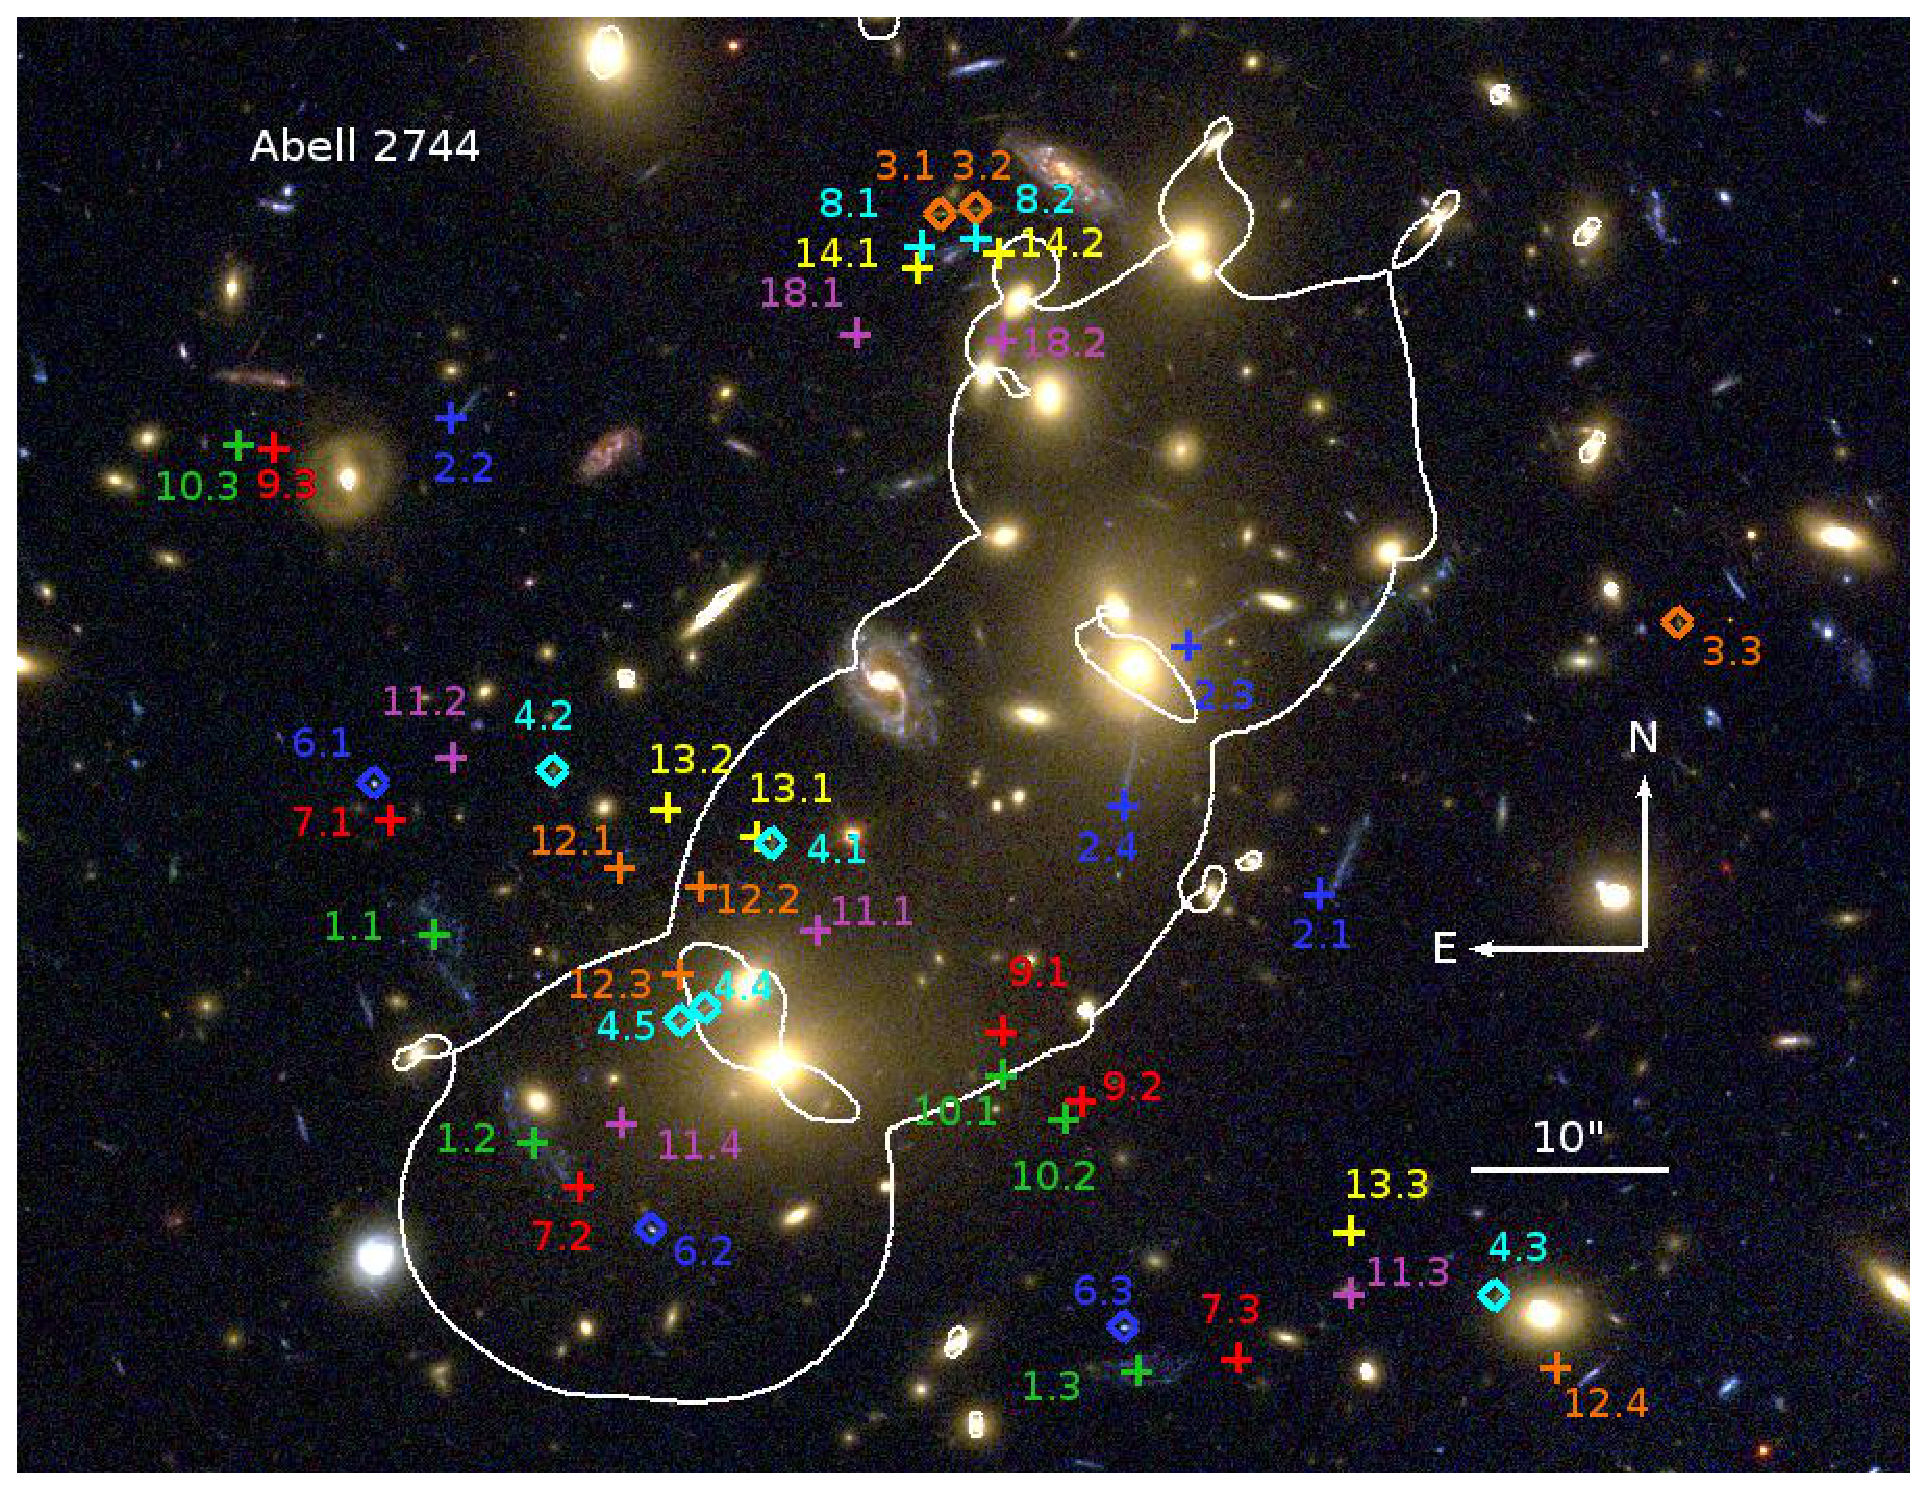
\includegraphics[width=0.85\textwidth]{Chap2/c2f1a.eps} \\
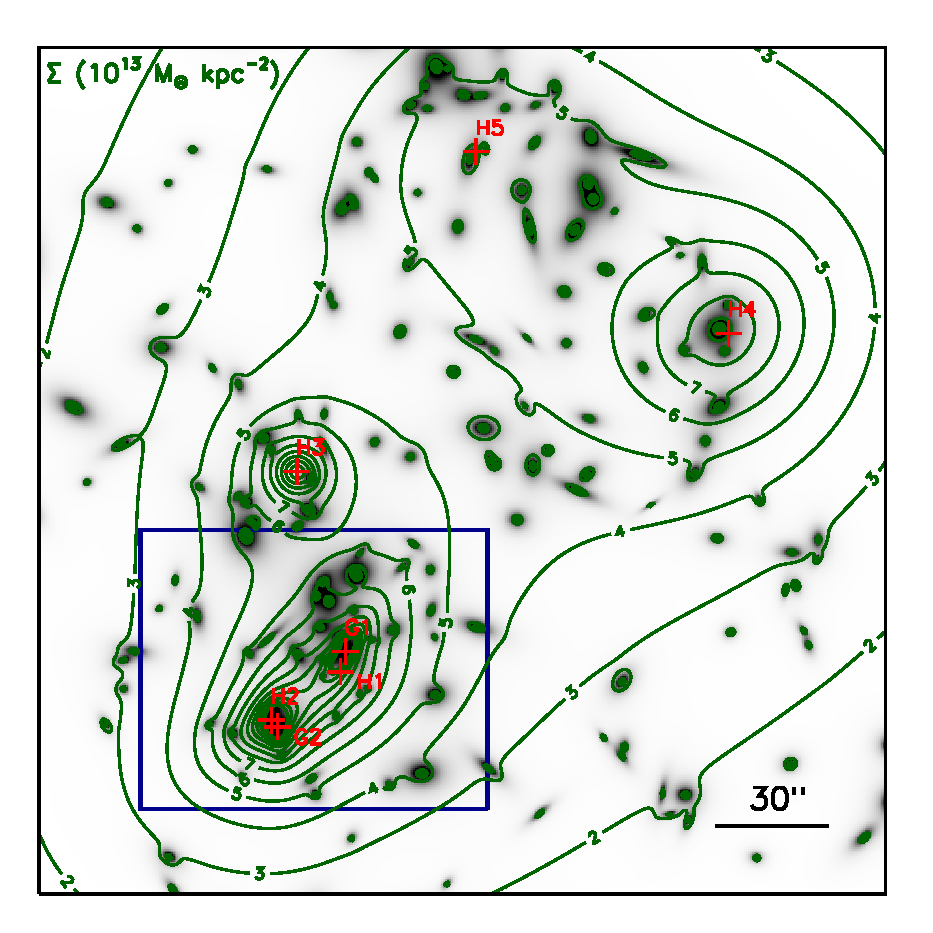
\includegraphics[height=0.28\textheight]{Chap2/c2f1b.eps}
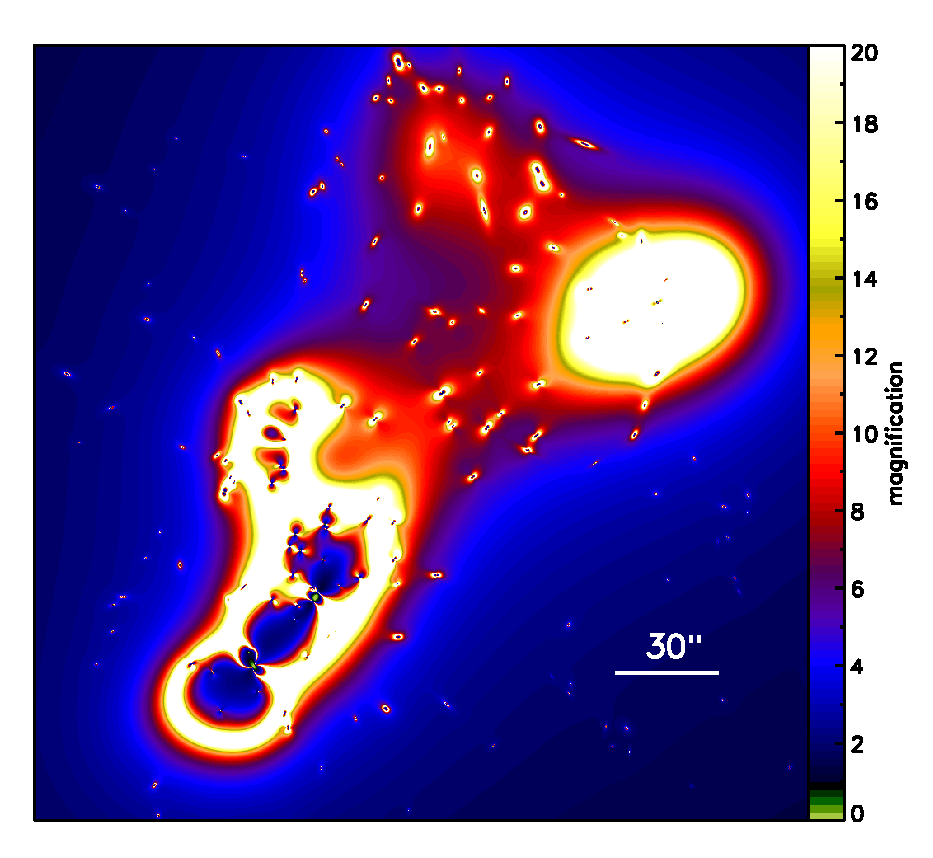
\includegraphics[height=0.28\textheight]{Chap2/c2f1c.eps}
\caption[Abell 2744 image constraints and critical curves]{Top: False color image of Abell 2744 from archival ACS imaging (red, F814W; green, F606W; blue, F435W) obtained as part of GO program 11689 (PI: R. Dupke). The locations of multiply imaged galaxies used as constraints in the model of Abell 2744 are overlaid. Diamonds designate image systems with spectroscopic redshifts, where crosses indicate that the redshift of the image system is left as a free parameter in the model. The critical curves (white) trace the region of high magnification for a source at $z=2$. Left: Contour map of the total surface mass distribution (in units of $10^{13}\ \mathrm{M_\odot \ kpc^{-2}}$) overlaid on the mass contained in cluster member galaxies. The spacing of the contours is linear. The locations and labels of each optimized halo (see Table \ref{app:tab:a2744_params}) are shown in red. The blue box indicates the field of view of the top image. Right: Absolute value of magnification in the image plane for a source at $z=9$.}
\label{chap2:fig:crit_a2744}
\end{figure*}

The majority of the image constraints are positioned within $<40$" of the cluster core (the region enclosed by HFF \hst\ WFC3/IR imaging), however, we include constraints for image \#16, which is about 2' northwest from the core to help constrain mass in that region. Since there are no known spectroscopic redshifts in this region of the lensing map, the redshift of this image system is not well constrained and is degenerate with other model parameters. Therefore, we fix the redshift to $z=3$, which lies in the middle of the range of its photometric redshifts ($2.6<\zphot<3.6$).

Our preliminary model (version 1, released in September 2013) included an image system, \#5, a low surface brightness arc stretching nearly 20" in the northern part of the cluster core. The image identifications were placed on brighter parts of the arc, but based on the monotonic color of the arc and overall low surface brightness, it is uncertain if these locations map to the same part of the source. There are also several galaxies along the line of sight to this arc that could potentially influence its lensing deflection. We exclude this image system from the model presented here based on its ambiguous identification. We find that the overall shape of this arc can be approximately replicated with the new best-fit model -- it is highly elongated and may be affected by lensing of cluster member galaxies. With deeper HFF imaging of this cluster, we may better understand this image system and include it in future models.

The complex mass distribution of Abell 2744 at $z=0.308$ is composed of five cluster or group-scale halos. We use two cluster-scale halos (H1, H2) to shape the mass distribution in the cluster core. In early model iterations, we find that the ellipticity of the halo (H1) lying closest to the brightest cluster galaxy (BCG) was near zero and not well constrained by the lensing evidence, so we assign it a circular halo. A third halo (H3) is located at $\sim50$" north-northeast of the cluster core close to an over density of cluster member galaxies, and is assigned a circular potential. We place a halo near image system \#16 (H4), which lies $\sim130$" northwest of the cluster core. A fifth halo (H5) is placed 140" north-northwest from the cluster core, which corresponds to an overdensity of cluster member galaxies in this region and a possible sub group of this cluster. The purpose of this halo is to add external shear to the lensing in the cluster core, and so its position and velocity dispersion are the only parameters that we can constrain, thus, we assign a circular potential to this halo and fix the $\rcore=150$ kpc. Weak lensing analyses by \citet{Merten:2011fk} and the Merten et al. preliminary HFF lens model reveal high surface mass densities in the regions outside of the HFF FOV, roughly in the areas where we place secondary halos far from the cluster core.

For cluster members, we assign halos at the cluster redshift and with parameters scaled by their magnitude in ACS F814W, such that an $\Lstar$ galaxy at the cluster redshift ($z=0.308$) has a magnitude $m_\star=18.50$. We freed the velocity dispersion, ellipticity, position angle, and $\rcut$ of the two brightest galaxies in the core for optimization, the central galaxy at $\alpha$=0:14:20.702, $\delta$=-30:24:00.62 and another galaxy at $\alpha$=0:14:22.091, $\delta$=-30:24:20.71. The BCG ellipticity tends toward unrealistically high values; in the final iteration we fix $e=0.8$.

We detect several galaxies with similar [F606W-F814W] colors, $\sim0.1$ mag blueward of the cluster red sequence. Our spectroscopic observation did not target any of these galaxies, since lensed galaxies in the core of the cluster received the highest priority. However, in examining the catalog of spectroscopic redshifts presented by \citet{Owers:2011rr}, we find one galaxy ($\alpha$=0:14:17.63, $\delta$=-30:22:40.58) with $z=0.239$. The color of the interloping galaxies is consistent with that of an elliptical galaxy at this redshift. We extend our red-sequence selection cut of cluster member galaxies to include these galaxies, as it is likely that these interloping galaxies contribute to the column mass of the cluster. Although not attempted here, this cluster is a clear case where a multi-plane lensing analysis may be necessary \citep[e.g., ][]{McCully:2014lr,Bayliss:2014fk,DAloisio:2013ul} in order to model this system.

Our lens model predicts a massive halo north-northeast of the cluster (H3), needed in order to reproduce the lensing of image systems \#3, 8, 14, and 18. Due to its mass and proximity to the main cluster halo, it produces a significant secondary critical curve component.  A visual inspection of the archival data show several low surface brightness arcs around the sub halo H3 which, at the depth of these data, cannot be confirmed strong lensing features. Nevertheless, new arcs may be confirmed in this region in the near future, with the new HFF data (e.g., the deep HFF observation of \MACSzerofour\ resulted in the identification of  $\sim200$ images in the ACS field by \citealt{Jauzac:2014qd}). We note that this region of the lens plane is not as well constrained as the rest of the cluster core, and may be prone to systematic errors in mass and magnification. Future work on this cluster lens model with more images should help to map the mass of this sub halo.

Figure~\ref{chap2:fig:crit_a2744} shows the best-fit critical curves for a source at $z=2$ and the multiply imaged galaxies that were used as constraints in the lens model of Abell 2744, overplotted on a color composite image of the cluster. The critical curves map regions of high magnification in the image plane. The magnification map at $z=9$ and the mass distribution of the cluster are displayed in the bottom panels.

We derive a cylindrical mass enclosing a projected radius of 250 kpc surrounding the core of Abell 2744 to be $M(r<250\ \mathrm{kpc})=2.43^{+0.04}_{-0.07}\times10^{14}\ \mathrm{M_\odot}$ (more mass measurements are given in Table \ref{chap2:tab:masses_aperture}), consistent with \citet{Merten:2011fk}, who derive $M(r<250\ \mathrm{kpc})=2.2\pm0.5\times10^{14}\ \mathrm{M_\odot}$ from weak and strong lensing evidence, which encompasses our value.

We note that since 14 of 15 image systems surround the region we refer to as the core, our strong lensing model best constrains the mass in this region of the cluster. Nonetheless, our model requires additional mass outside of the core to explain the lensing of these images. Abell 2744 is an actively merging cluster \citep{Merten:2011fk}, and the complexity of its multiple halo components and unrelaxed state make this cluster a challenge to model in the entirety of the HFF FOV. The accuracy of the model will improve after the HFF observations are complete, and additional multiple-image systems are identified in other regions of the image plane.

% MACS 0416
\subsection{\MACSzerofour}

The lensed galaxies that were used as constraints in the model were originally identified by \citet[see Table \ref{app:tab:m0416_arcs} in the Appendix]{Zitrin:2013lr}. We fix the redshift of image system \#1 to the spectroscopic redshift from \citeauthor{Zitrin:2013lr} and systems \#2, 3, 4, 7, 10, 13, 14, 16, and 17 to the spectroscopic redshifts obtained under VLT program 186.A-0798 \citep{Balestra:2013uq,Grillo:2014uq}.

The model of \MACSzerofour\ at $z=0.396$ consists of two cluster-scale components, halos assigned to each cluster member galaxy within the ACS FOV, and a foreground galaxy. We allow all parameters of the cluster-scale halos to be optimized with the exception of cut radius. The scaling relation for the cluster member galaxies is based on their magnitude in ACS F775W with $m_\star=19.33$. The parameters of the BCG cannot be constrained during optimization, so they are fixed to the values derived from the scaling relations. We also allow the velocity dispersion of the galaxy near images 5.2 and 5.3 ($\alpha$=4:16:07.786, $\delta$=-24:04:06.51; G2) to be a free parameter in the lens model, as it contributes to the cluster-boosted galaxy-galaxy lensing in image system \#5. While this galaxy has similar color to the cluster member galaxies, it did not make the red-sequence cut on first pass. The extracted shape of the galaxy did not match well with observations due to contamination by other galaxies, so we assign a circular PIEMD halo instead. We assign a halo to the bright foreground galaxy at ($\alpha$=4:16:06.817, $\delta$=-24:05:08.44; F1) and allowed it to vary in core and cut radii and velocity dispersion, as this galaxy may deviate from the scaling relations typical of elliptical galaxies at the cluster redshift. Early iterations converged to a very large cut radius of this galaxy which is not well constrained, so we arbitrarily fixed it to 1500 kpc. Figure~\ref{chap2:fig:crit_m0416} shows the best-fit critical curves, modeling constraints, mass distribution, and magnification map for the \MACSzerofour\ lens model.

\begin{figure*}[h]
\centering
\includegraphics[width=0.85\textwidth]{Chap2/c2f2a.eps}\\
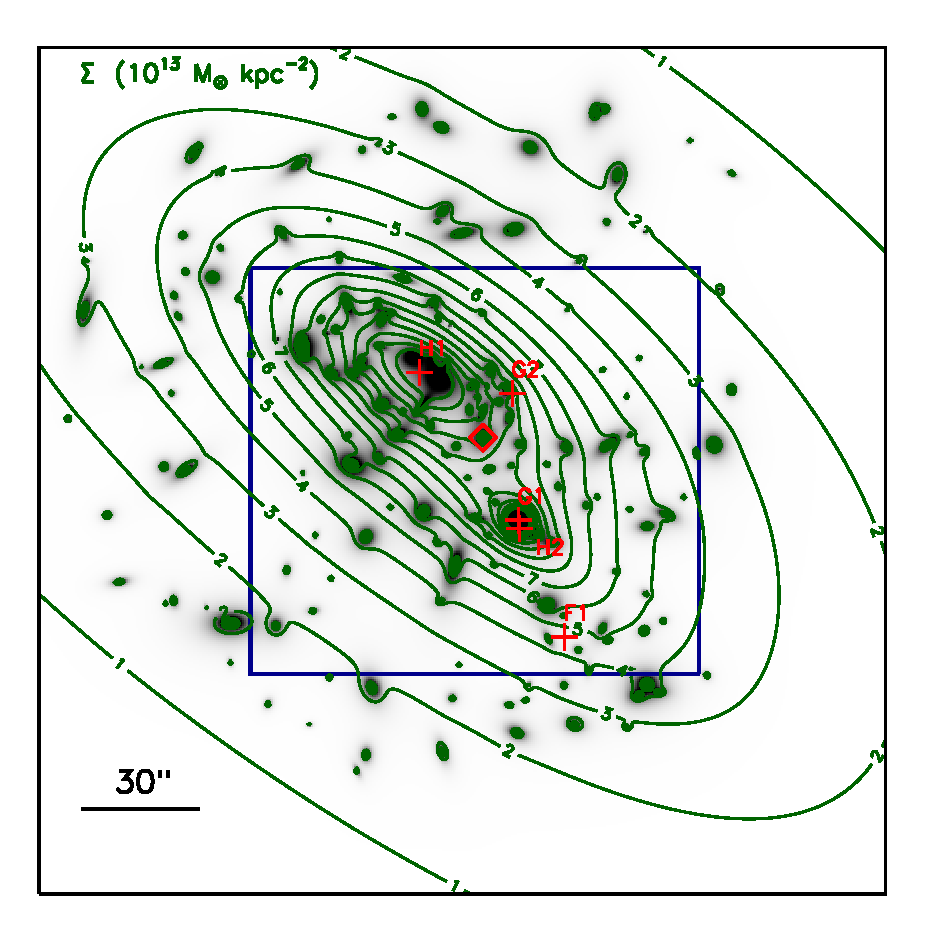
\includegraphics[height=0.28\textheight]{Chap2/c2f2b.eps}
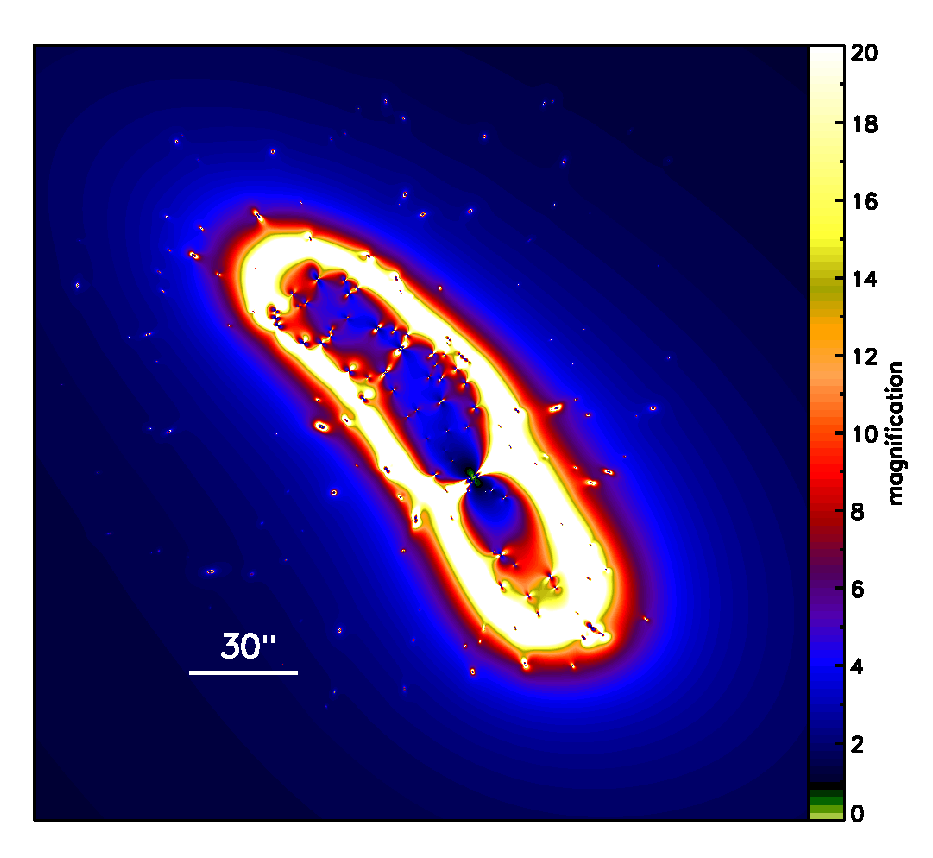
\includegraphics[height=0.28\textheight]{Chap2/c2f2c.eps}
\caption[\MACSzerofour\ image constraints and critical curves]{Top: False color image of \MACSzerofour\ from WFC3/IR (red; F105W, F110W, F125W, F140W, and F160W), ACS (green; F435W, F475W, F606W, F625W, F775W, F814W, and F850LP), and WFC3/UVIS (blue; F225W, F275W, F336W, and F390W) imaging. Labels are the same as in Figure~\ref{chap2:fig:crit_a2744}. Left: Contour map of the total surface mass distribution (in units of $10^{13}\ \mathrm{M_\odot \ kpc^{-2}}$) overlaid on the mass contained in cluster member galaxies. The spacing of the contours is linear. The locations and labels of each optimized halo (see Table~\ref{app:tab:m0416_params}) are shown in red crosses. The red diamond indicates the location of the reference point. The blue box indicates the field of view of the top image. Right: Absolute value of magnification in the image plane for a source at $z=9$.}
\label{chap2:fig:crit_m0416}
\end{figure*}

We compute $M(r<250\ \mathrm{kpc})=1.77^{+0.31}_{-0.13}\times10^{14}\ \mathrm{M_\odot}$ and $M(r<500\ \mathrm{kpc})=4.05^{+0.90}_{-0.32}\times10^{14}\ \mathrm{M_\odot}$ for the mass of \MACSzerofour. We note that a weak lensing model by \citet{Gruen:2014lr} yields $M(r<250\ \mathrm{kpc})=1.8\pm0.3\times10^{14}\ \mathrm{M_\odot}$ and $M(r<500\ \mathrm{kpc})=3.8\pm0.7\times10^{14}\ \mathrm{M_\odot}$, which are in agreement with our model. We measure $M(<\mathrm{crit})=0.80^{+0.12}_{-0.06}\times10^{14}\ \mathrm{M_\odot}$ for the mass within the $z=2$ critical curve. \citet{Zitrin:2013lr} report the mass within the critical curve of the main arc (at $z=1.896$) to be $M(<\mathrm{crit})=1.25\pm0.09\times10^{14}\ \mathrm{M_\odot}$. The critical curves for both models enclose nearly the same amount of area (0.58 $\square'$). The discrepancy between the two models can possibly be explained by the fact that the \citet{Zitrin:2013lr} model was computed prior to the spectroscopic confirmations of several lensed galaxies in this cluster; therefore, leaving the critical curve less constrained in some regions of the map. The redshift predictions of the image systems in the \citet{Zitrin:2013lr} model are systematically higher than the spectroscopic redshifts we included in the model we present here. The source redshifts of the images place a strong constraint on the slope of the mass distribution, and higher redshift predictions require larger mass within the same critical curve area. We discuss the implications of including spectroscopic redshifts on the derived lens model of clusters later in \S \ref{chap2:sec:specz}.

% MACS 0717
\subsection{\MACSzeroseven}

We use the multiple images initially identified by \citet{Zitrin:2009qy} and later revised by \citet{Limousin:2012fj} (Table \ref{app:tab:m0717_arcs} in the Appendix). The coordinates of the lensed galaxies have been matched to the CLASH imaging data. We fix the redshifts of image systems \#1, 3, 13, 14, and 15 to the spectroscopic redshifts reported by \citet{Limousin:2012fj}.

The mass distribution of \MACSzeroseven\ at $z=0.545$ is best represented by several separate halo components, consistent with the findings of an X-ray / optical study by \citet{Ma:2009gf}. Besides the lensing evidence, the locations of the halos are observationally motivated as they lie close to overdensities of cluster member galaxies. We include cluster member galaxies in the model, as selected by \citet{Limousin:2012fj}, with $m_\star=20.66$ in ACS F814W. We allow the velocity dispersion and cut radius of the cluster galaxy at ($\alpha$=7:17:35.646, $\delta$=+37:45:17.40; G1) to be optimized by the model. A foreground galaxy at ($\alpha$=7:17:37.224,$\delta$=+37:44:22.99; F1) is also included in the model, with a circular PIEMD halo, and free cut radius and velocity dispersion parameters. The core radius of this galaxy could not be constrained, so it is fixed arbitrarily to the value at the cluster redshift based on the scaling relation. Figure~\ref{chap2:fig:crit_m0717} shows the inputs to and details of the lens model for this cluster.

\begin{figure*}[h]
\centering
\includegraphics[width=0.85\textwidth]{Chap2/c2f3a.eps} \\
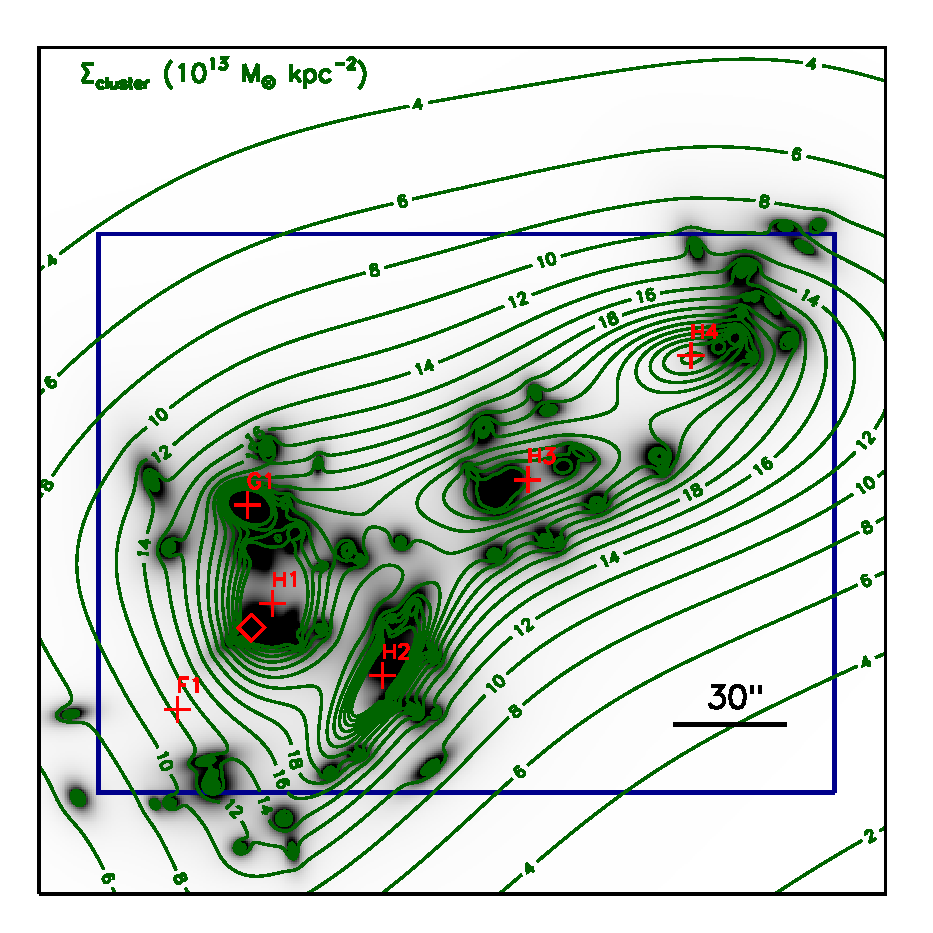
\includegraphics[height=0.28\textheight]{Chap2/c2f3b.eps}
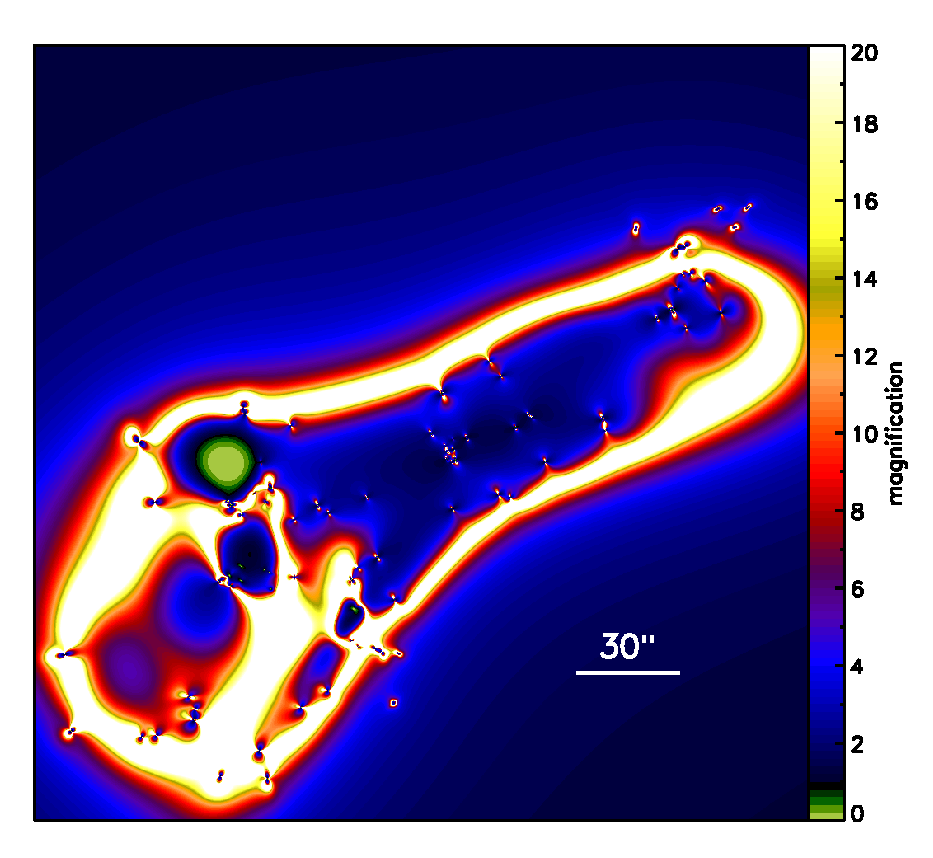
\includegraphics[height=0.28\textheight]{Chap2/c2f3c.eps}
\caption[\MACSzeroseven\ image constraints and critical curves]{Top: False color image of \MACSzeroseven\ from ACS imaging (red, F814W; green, F606W; blue, F435W). Labels are the same as in Figure~\ref{chap2:fig:crit_a2744}. Left: Contour map of the total surface mass distribution (in units of $10^{13}\ \mathrm{M_\odot \ kpc^{-2}}$) of the cluster overlaid on the mass contained in cluster member galaxies. The spacing of the contours is linear. The locations and labels of each optimized halo (see Table \ref{app:tab:m0717_params}) are shown in red crosses. The red diamond indicates the location of the reference point. The blue box indicates the field of view of the top image. Right: Absolute value of magnification in the image plane for a source at $z=9$.}
\label{chap2:fig:crit_m0717}
\end{figure*}


% changes masses in this paragraph!!!!!
It is likely that this merging system has a more complex mass distribution that cannot be accurately represented by parameterized halos; nevertheless, the resulting image plane rms for the constraints used in this model is good (0.38"). We note that a direct, halo-to-halo comparison with the \citet{Ma:2009gf} findings is not meaningful, for two reasons: the PIEMD velocity dispersion is not defined as the measured velocity dispersion \citep[see][]{Eliasdottir:2007ve}, and the halos have different geometry, positions, and fragmentation. Nevertheless, we can directly measure the mass from our model within each area associated with the subclusters defined by \citet{Ma:2009gf} We find the mass within the regions labeled A, B, C, and D in \citet{Ma:2009gf} are $M = 5.5^{+0.3}_{-0.4}, 6.9\pm0.2, 16.6^{+0.4}_{-0.6}, 6.5^{+0.1}_{-0.2}\times10^{13}\ \mathrm{M_\odot}$, respectively. The values for cores A, C, and D correspond well with the observed velocity dispersions within errors, taking for simplicity their viral masses. The derived mass for core B is slightly higher than what is inferred from the observations. \citet{Ma:2009gf} find that this core is moving at a high radial velocity ($\Delta v>3000 \ \mathrm{km\ s^{-1}}$) relative to the cluster core, near the infall velocity. Estimating the mass from virial assumptions may not be best in this scenario, which could account for the discrepancy in the mass estimates. The agreement between the completely independent lensing evidence and dynamics suggests that future modeling efforts can benefit from including the measured velocity dispersion as a Bayesian constraint. 

% and masses in this paragraph too!
\MACSzeroseven\ is by far the most massive cluster in the HFF, with a mass $M(r<500\ \mathrm{kpc})=8.68^{+0.27}_{-0.13}\times10^{14}\ \mathrm{M_\odot}$. We find $M(<\mathrm{crit})=5.27^{+0.20}_{-0.11}\times10^{14}\ \mathrm{M_\odot}$ for the mass enclosed by the $z=2$ critical curve, yielding an impressive effective Einstein radius of $\theta_E=50.1^{+0.8}_{-0.3}"$. This critical curve encloses a factor of more than two greater area than any other cluster in the HFF, and should prove to be an efficient lens of background galaxies. Additionally, we find the mass within the $z=2.5$ critical curve to be $M(<\mathrm{crit})=5.91^{+0.20}_{-0.08}\times10^{14}\ \mathrm{M_\odot}$. Our measurement differs significantly from \citet{Zitrin:2009qy}, who find the mass enclosed by the critical curve at $z=2.5$ to be $M(<\mathrm{crit})=7.4\pm0.5\times10^{14}\ \mathrm{M_\odot}$. Their lens model uses fewer image constraints and is not supported by spectroscopic or photometric redshifts. As a result, the critical curve for $z=2.5$ may change positions in the image plane based on the input redshifts of the image constraints, causing the discrepancy between the two models. We discuss the effects of model redshifts as inputs in \S \ref{chap2:sec:specz}.

% MACS 1149
\subsection{\MACSeleven}

We use as constraints the strongly lensed image lists from \citet{Smith:2009lr}, \citet{Zitrin:2009kx}, and \citet{Zheng:2012fk} supplemented by unpublished identifications made by Adi Zitrin (priv. comm.).$^{\ref{note}}$ We consolidate all lists of images; the complete list is shown in Table \ref{app:tab:m1149_arcs} in the Appendix.  We fix the redshifts of systems \#1, 2, and 3 to the spectroscopic redshifts reported by \citet{Smith:2009lr}. Our preliminary model (version 1, released September 2013) included an image system labelled \#12 whose high image-plane rms of 4.6" indicates a potential misidentification. Excluding this system as a constraint, the model presented here predicts a redshift of $z>3$ for the two outer-most images of this image set, in stark contrast to the photometric estimate of $z\sim1$. The nature of this system may be better understood with the full HFF depth and spectroscopic confirmation.

The lens model of \MACSeleven\ at $z=0.543$ consists of two dark matter halos, one lying close to the BCG (H1) and the other located near an overdensity of cluster galaxies 100" north of the cluster center (H2). We include the cluster member galaxies selected by \cite{Smith:2009lr}, with $m_\star=20.3$ from K band imaging. We allow only the position, velocity dispersion, and cut radius of the second halo to vary in the model. We include the velocity dispersion and cut radii of the BCG ($\alpha$=11:49:35.695,$\delta$=+22:23:54.70) and cluster member galaxy at ($\alpha$=11:49:37.541,$\delta$=+22:23:22.51; G1) as free parameters. We also include a galaxy-scale halo north of the cluster (G2) accounting for the lensing of image systems \#9 and \#10, due to the galaxy-galaxy lensing boosted by the mass from the dark matter halo of the cluster. Since neither of these two systems have spectroscopic redshifts, we do not have enough constraints to attempt to model both the individual galaxy plus other substructure in that vicinity, which is essentially isolated from the rest of the cluster. Instead, we use a single halo with position priors matching the galaxy at ($\alpha$=11:49:36.926,$\delta$=+22:25:35.82). The model requires an unrealistically high ellipticity, indicating that more substructure may be needed; we thus fix it to $e=0.8$ and leave the position angle, velocity dispersion, and cut radius as free parameters. The necessity of optimizing this halo in the model far away from the majority of modeling constraints suggests the presence of significant substructure in part of the lens plane. The critical curves, image constraints, mass distribution, and magnification map for this cluster are shown in Figure~\ref{chap2:fig:crit_m1149}.

\begin{figure*}[h]
\centering
\includegraphics[width=0.85\textwidth]{Chap2/c2f4a.eps} \\
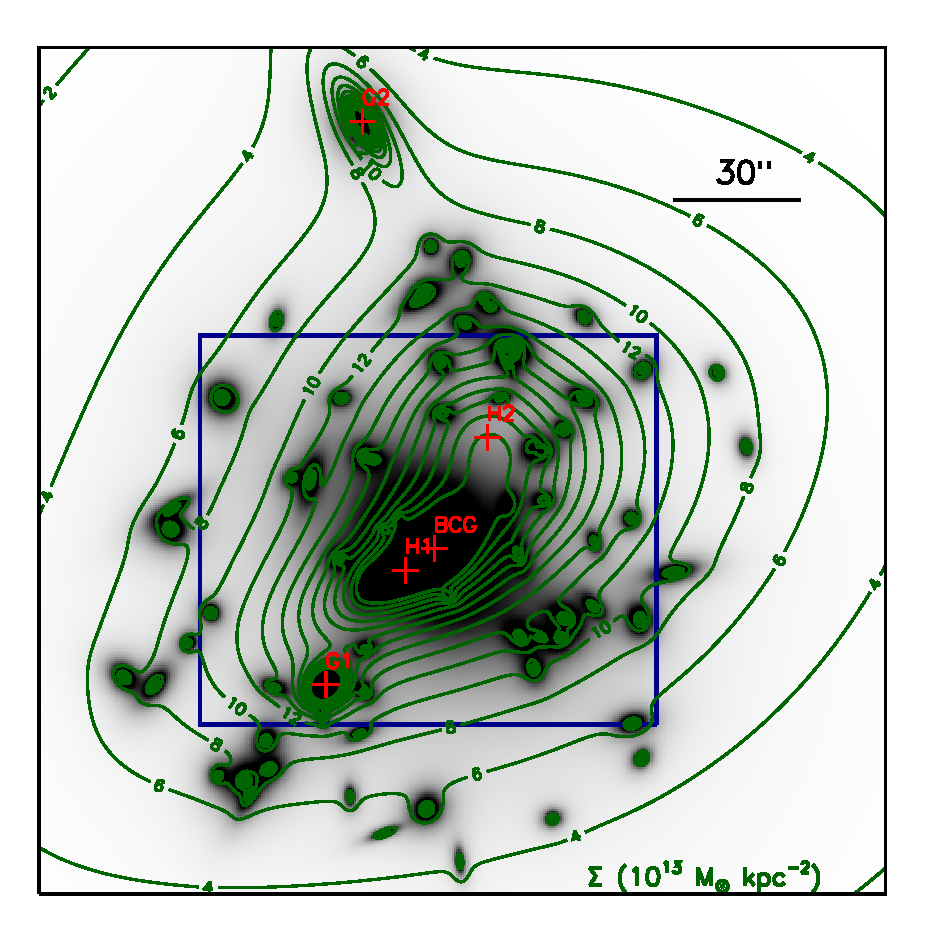
\includegraphics[height=0.28\textheight]{Chap2/c2f4b.eps}
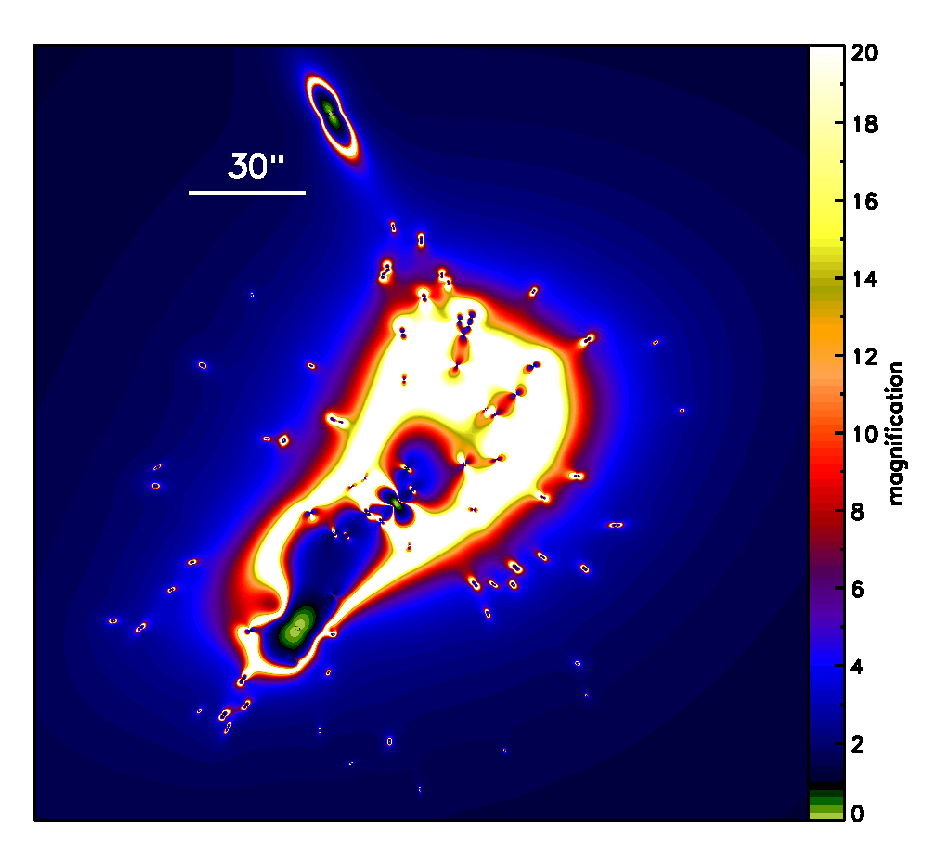
\includegraphics[height=0.28\textheight]{Chap2/c2f4c.eps}
\caption[\MACSeleven\ image constraints and critical curves]{Top: False color image of \MACSeleven\ from ACS imaging (red, F814W; green, F606W; blue, F435W). Labels are the same as in Figure~\ref{chap2:fig:crit_a2744}. Left: Contour map of the total surface mass distribution (in units of $10^{13}\ \mathrm{M_\odot \ kpc^{-2}}$) overlaid on the mass contained in cluster member galaxies. The spacing of the contours is linear. The locations and labels of each optimized halo (see Table \ref{app:tab:m1149_params}) are shown in red. The blue box indicates the field of view of the top image. Right: Absolute value of magnification in the image plane for a source at $z=9$.}
\label{chap2:fig:crit_m1149}
\end{figure*}

We compute a cylindrical mass at the core of \MACSeleven\ of $M(r<500\mathrm{kpc})=5.98^{+0.59}_{-0.25}\times10^{14}\ \mathrm{M_\odot}$. We can directly compare this value with the model by \citet{Smith:2009lr}, who find $M(r<500\mathrm{kpc})=6.7\pm0.4\times10^{14}\ \mathrm{M_\odot}$. In fact, the \citet{Smith:2009lr} and our model were constructed independently with \texttt{LENSTOOL} and resulted in similar locations of cluster halo components in the lens plane. However, the previous model was built with fewer identified image systems. Our model includes 35 images from 12 uniques sources, whereas \citet{Smith:2009lr} identified 19 images from 6 unique, multiply imaged sources. We find $M(<\mathrm{crit})=1.12^{+0.01}_{-0.04}\times10^{14}\ \mathrm{M_\odot}$ for the mass enclosed by the $z=2$ critical curve ($0.40^{+0.01}_{-0.02}$ $\square'$), which does not agree with \citet{Zitrin:2011qy}, who find $M(<\mathrm{crit})=1.71\pm0.20\times10^{14}\ \mathrm{M_\odot}$ (0.63 $\square'$). We note that the \citet{Zitrin:2011qy} model does again not include any spectroscopic or photometric redshifts, have a different set of multiple image identifications, and do not treat their image redshift constraints as free parameters. We refer the reader to the discussion in \citet{Smith:2009lr}, where they rule out the inner slope of the surface mass density profile of the \citet{Zitrin:2011qy} model by $7\sigma$. This example demonstrates how different modeling inputs can result in significantly different lens models. We will discuss this further in \S \ref{chap2:sec:specz}.

% ABELL S1063
\subsection{Abell S1063}
\label{chap2:sec:results_as1063}

We constrain the lens model of Abell S1063 with a combination of the images identified by \citet{Monna:2014lr} and Johan Richard (priv. comm.).$^{\ref{note}}$ For features common to both catalogs, we use the \citet{Monna:2014lr} coordinates. We fix the redshifts of systems \#1, 2, 5, 6 to the spectroscopic redshifts measured in this work and by  \citet{Richard:2014gf}, \#12 to the spectroscopic redshift measured by \citet{Balestra:2013uq,Boone:2013lr}, and the redshift of \#11 to the spectroscopic redshift we measured in this work.

The lens model for Abell S1063 at $z=0.348$ consists of three cluster-scale halos: a central halo located near the BCG (H1), a halo $\sim400"$ northeast of the cluster center (H2), and another $\sim100"$ to the south (H3). We assign circular potentials with fixed $r_\mathrm{core}=50\ \mathrm{kpc}$ to the secondary halos since there are no strong lensing constraints in this vicinity to constrain the inner slope of the density profiles. We can only constrain the mass and position of these halos and the slope of the density profiles at the location of the multiple images, which allows us to place constraints on the velocity dispersion and position of the halos. We included all cluster member galaxies within the ACS FOV, with $m_\star=18.82$ in ACS F814W. We set the velocity dispersions of the BCG and three other cluster member galaxies as free parameters in the model. These three galaxies lie close to image systems \#1 ($\alpha$=22:48:46.925,$\delta$=-44:31:33.60; G1), \#11 ($\alpha$=22:48:41.223,$\delta$=-44:32:25.96; G2), and \#16 ($\alpha$=22:48:39.984,$\delta$=-44:32:05.33; G3). Image constraints, critical curve, mass distribution, and magnification map of the lens model are shown in Figure~\ref{chap2:fig:crit_as1063}.

\begin{figure*}[h]
\centering
\includegraphics[width=0.85\textwidth]{Chap2/c2f5a.eps} \\
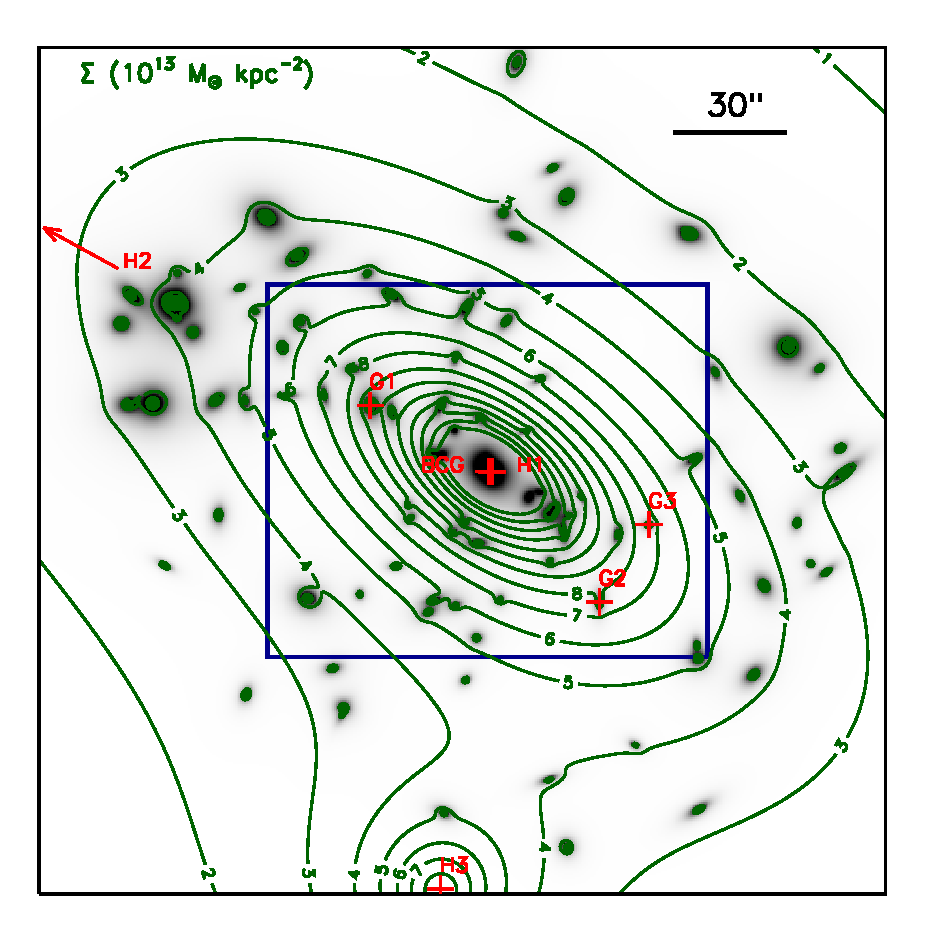
\includegraphics[height=0.28\textheight]{Chap2/c2f5b.eps}
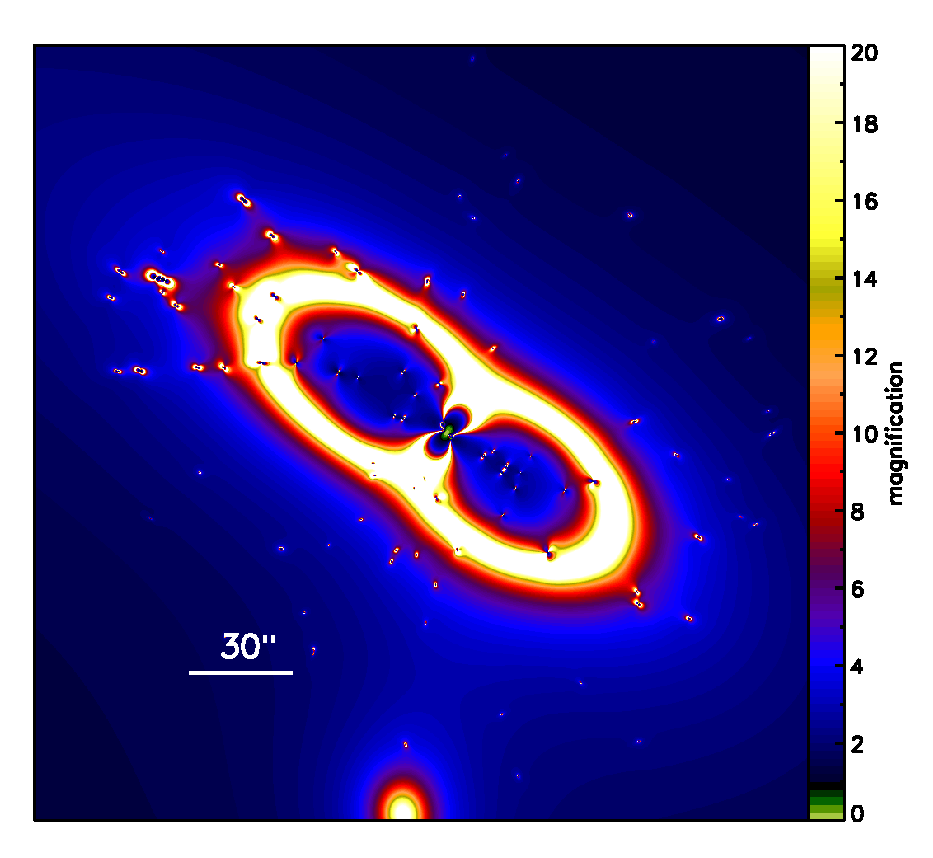
\includegraphics[height=0.28\textheight]{Chap2/c2f5c.eps}
\caption[Abell S1063 image constraints and critical curves]{Top: False color image of Abell S1063 from ACS imaging (red, F814W; green, F606W; blue, F435W).  Labels are the same as in Figure~\ref{chap2:fig:crit_a2744}. Left: Contour map of the total surface mass distribution (in units of $10^{13}\ \mathrm{M_\odot \ kpc^{-2}}$) overlaid on the mass contained in cluster member galaxies. The spacing of the contours is linear. The locations and labels of each optimized halo (see Table \ref{app:tab:as1063_params}) are shown in red. The blue box indicates the field of view of the top image. Right: Absolute value of magnification in the image plane for a source at $z=9$.}
\label{chap2:fig:crit_as1063}
\end{figure*}

The two outer cluster-scale halos (H2 and H3) are new additions to the first version of the model released in September 2013, and are motivated by our spectroscopic redshift measurement of image system \#11. In version 1 of this model, the soft prior that was set by the photometric redshifts of system \#11 and other images in its vicinity allowed the model to converge to a solution with less complexity, by predicting lower source redshifts than the photometric redshift estimates.  We discuss this further in \S \ref{chap2:sec:specz}.  We note that the outer halos, which are strictly motivated by the lensing constraints, coincide with higher densities of galaxies in the northeastern most part of the \hst\ FOV. Independent weak lensing models (\citet{Gruen:2013lr} and the Merten et al. preliminary HFF lens model) show evidence for mass in the same regions as these new halos. These structures are outside the \hst\ FOV, but may correspond to galaxy over densities in the wide field imaging used by \citet[][Figure~15 of that publication]{Gruen:2013lr}.

We compute cylindrical masses of $M(r<250\ \mathrm{kpc})=2.68^{+0.03}_{-0.05}\times10^{14}\ \mathrm{M_\odot}$ and $M(r<500\ \mathrm{kpc})=6.39^{+0.14}_{-0.32}\times10^{14}\ \mathrm{M_\odot}$. This cluster has a large effective Einstein radius, $\theta_E=29.8^{+0.1}_{-0.3}$", making it a very efficient lens of background sources. In the first strong lensing analysis of this cluster, \citet{Monna:2014lr} find $\theta_E=29.9^{+1.7}_{-1.9}$" and $M(<\mathrm{crit})=1.24\pm0.01\times10^{14}\ \mathrm{M_\odot}$ for $z=2$, and also compute $M(r<250\ \mathrm{kpc})=2.8\pm0.1\times10^{14}\ \mathrm{M_\odot}$ and $M(r<500\ \mathrm{kpc})=6.3\pm0.3\times10^{14}\ \mathrm{M_\odot}$. From weak lensing analysis, \citet{Gruen:2013lr} find $M(r<250\ \mathrm{kpc})=2.3^{+0.3}_{-0.2}\times10^{14}\ \mathrm{M_\odot}$ and $M(r<500\ \mathrm{kpc})=6.1^{+0.6}_{-0.7}\times10^{14}\ \mathrm{M_\odot}$. All three of these analyses are in excellent agreement. This cluster has been studied in detail in the optical and x-ray \citep{Cruddace:2002vn,Maughan:2008rt,Comis:2011fr,Gomez:2012yq} and in exploring its SZ effect \citep{Plagge:2010ys}. Many of these studies indicate a complex mass distribution beyond the FOV of existing \hst\ data for this cluster.

% ABELL 370
\subsection{Abell 370}

We use the multiple images identified by \citet{Richard:2010wd} and  \citet{Richard:2014gf}$^{\ref{note}}$ as constraints in our lens model, and fix the redshifts of systems \#1, 2, 3, 4, and 6 to the spectroscopic redshifts measured by these groups. The list of image constraints used in the model can be found in Table \ref{app:tab:a370_arcs} in the Appendix.

We model Abell 370 at $z=0.375$ with two cluster-scale dark matter halos and cluster member galaxies, for which we scale the parameters using the ACS F814W magnitudes with $m_\star=19.04$. We allow the velocity dispersion of the BCG ($\alpha$=2:39:53.125, $\delta$=-1:34:56.42) to be optimized. Early model iterations indicate that the core and cut radii of this galaxy cannot be constrained by the lensing evidence, so we leave these parameters fixed to the scaled values. The perturbing galaxy at ($\alpha$=2:39:52.595, $\delta$=-1:35:06.22; G1) is responsible for creating the swallowtail caustic which produces the quintuply-imaged giant arc (image system \#2). We began by allowing all parameters of the galaxy except position to vary in the model; however, we found that only velocity dispersion, position angle, and ellipticity could be constrained. The ellipticity of the galaxy is forced by the constraints to be unrealistically high for an elliptical galaxy, so we fixed the value to $e=0.8$ as opposed to the value matching the light distribution and leave velocity dispersion and position angle as free parameters. Figure~\ref{chap2:fig:crit_m0416} shows the critical curve, image constraints, mass distribution, and magnification map of this cluster.

\begin{figure*}[h]
\centering
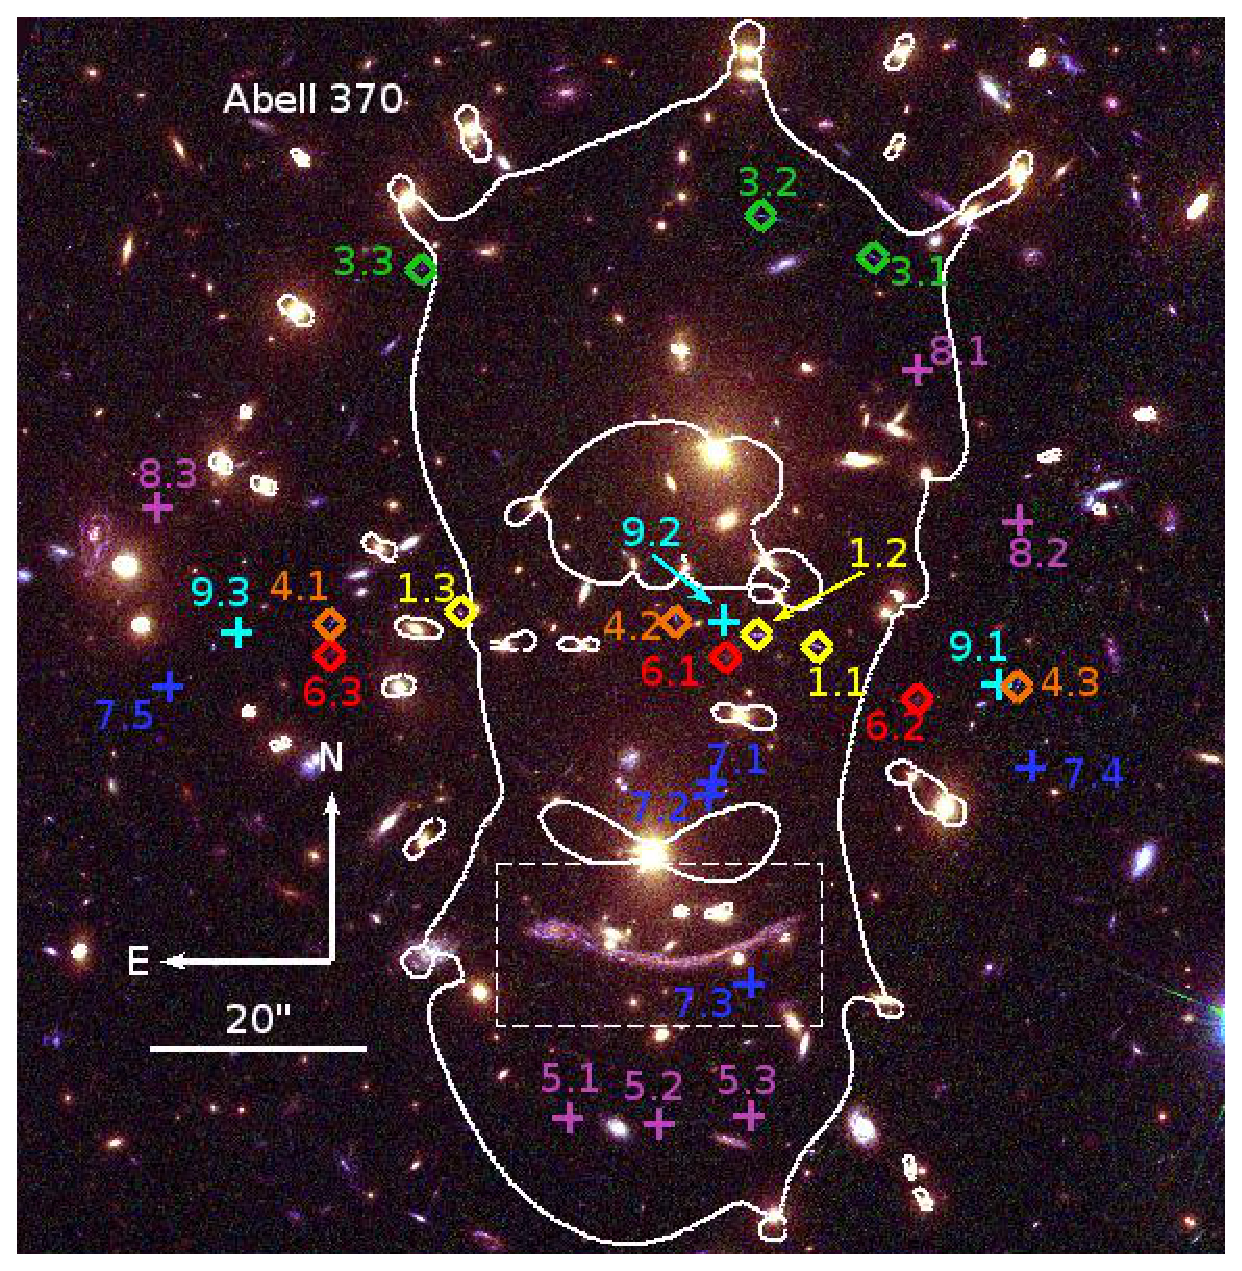
\includegraphics[width=0.55\textwidth]{Chap2/c2f6a.eps}
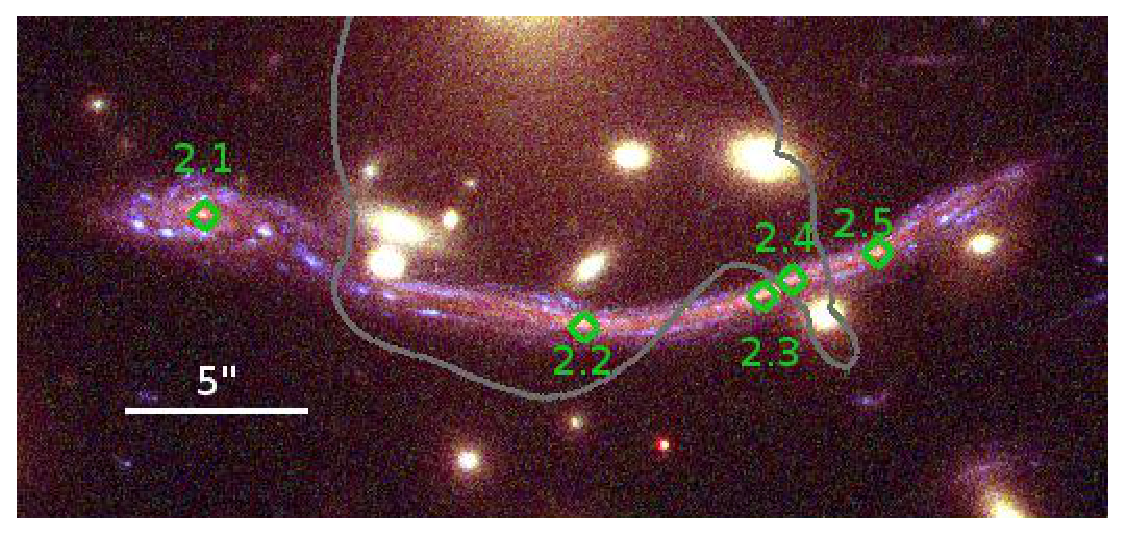
\includegraphics[width=0.4\textwidth]{Chap2/c2f6d.eps}
\\
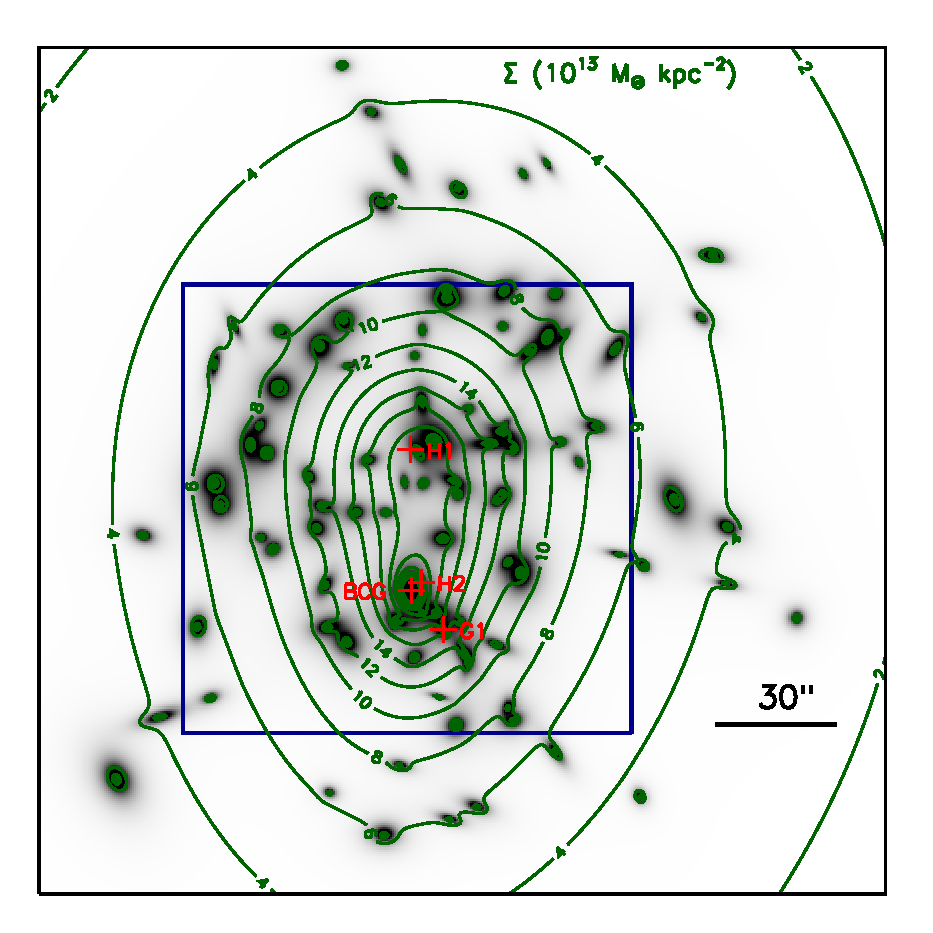
\includegraphics[height=0.28\textheight]{Chap2/c2f6b.eps}
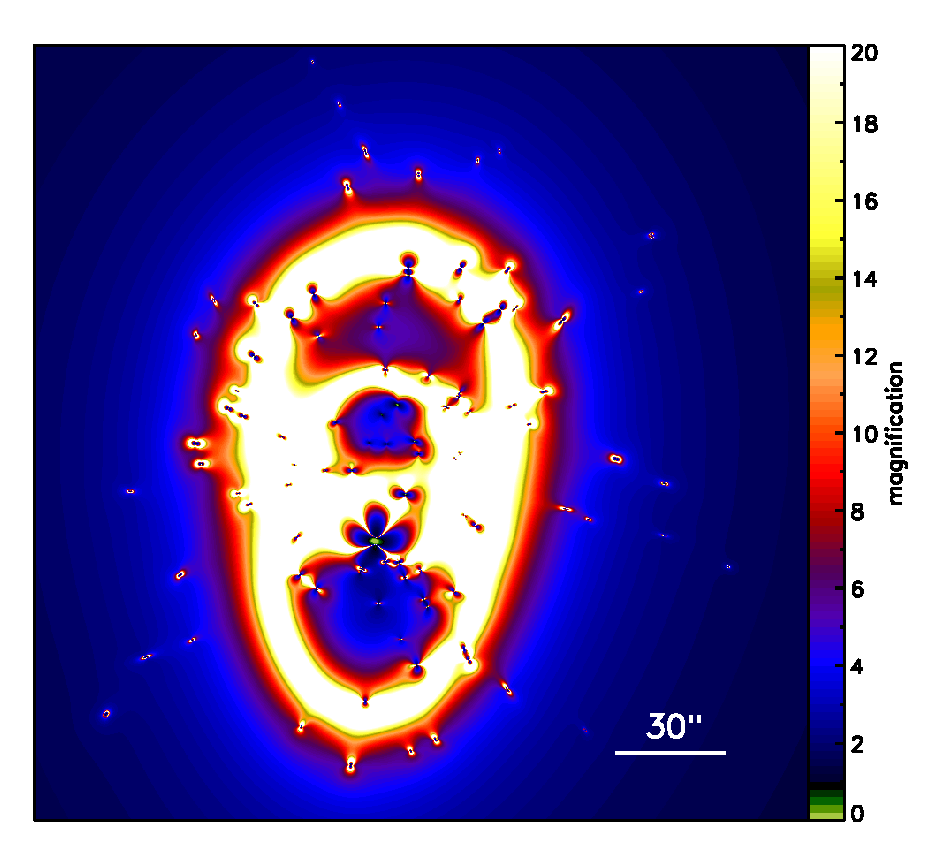
\includegraphics[height=0.28\textheight]{Chap2/c2f6c.eps}
\caption[Abell 370 image constraints and critical curves]{Top left: False color image of Abell 370 from archival ACS imaging (red, F814W; green, F606W; blue, F435W) by HST SM4 ERO program 11597 (PI: K. Noll), program 11591 (PI:. J.-P. Kneib), program 11582 (PI: A. Blain), and program 11108 (PI: E. Hu).  Labels are the same as in Figure~\ref{chap2:fig:crit_a2744}. Top right: The inset shows the image constraints of the giant arc (image system \#2); the gray line is the critical curve corresponding to the spectroscopic redshift of this arc, $z=0.725$. Bottom left: Contour map of the total surface mass distribution (in units of $10^{13}\ \mathrm{M_\odot \ kpc^{-2}}$) overlaid on the mass contained in cluster member galaxies. The spacing of the contours is linear. The locations and labels of each optimized halo (see Table \ref{app:tab:a370_params}) are shown in red. The blue box indicates the field of view of the top image. Bottom right: Absolute value of magnification in the image plane for a source at $z=9$.}
\label{chap2:fig:crit_a370}
\end{figure*}

We compute masses of $M(r<250\ \mathrm{kpc})=3.48^{+0.02}_{-0.04}\times10^{14}\ \mathrm{M_\odot}$ within 250 kpc of the cluster center and $M(<\mathrm{crit})=2.36^{+0.02}_{-0.05}\times10^{14}\ \mathrm{M_\odot}$ within the $z=2$ critical curve for Abell 370, respectively. The strong lensing \texttt{LENSTOOL} model by \citet{Richard:2010wd} yields $M(r<250\ \mathrm{kpc})=3.8\pm0.2\times10^{14}\ \mathrm{M_\odot}$ and $M(<\mathrm{crit})=2.82\pm0.15\times10^{14}\ \mathrm{M_\odot}$  ($z=2$ critical curve). Our values differ slightly from those of \citeauthor{Richard:2010wd} Both models used similar image constraints; however, our model is up to date with the latest spectroscopic redshifts by  \citet{Richard:2014gf}, which may account for the discrepancy. These measurements are responsible for producing a narrower range of uncertainties on the derived masses in our model compared to the earlier \citeauthor{Richard:2010wd} model.


%==================================================================================
%   DISCUSSION AND CONCLUSIONS
%==================================================================================
\section{Discussion and future work}
\label{chap2:sec:discussion}

The detailed lens models in this work are based on archival \hst\ data that exist prior to the deep imaging of the HFF in \hst\ Cycles 21-23, and on all the known spectroscopic redshifts of lensed galaxies as of this publication. These models can be used for deriving magnification estimates for background sources as well as for studying the mass distribution approximately within the footprint of these archival data (within 3' of the cluster center). In this section, we highlight a few caveats and discuss the implications of some possible uncertainties and systematics on the model parameters and magnification estimates; we also outline future work that would advance our understanding of these issues. 

\subsection{Precision in lensing maps}
\label{chap2:sec:precision}

Our models of the HFF derive magnifications most precisely within the strong lensing regime, approximately the region enclosed by the strongly lensed galaxies (typically within $\sim100"$ of cluster center). Therefore, the regions within a few arcseconds of any images used as constraints in our model will have the most precise magnifications, especially if those images had spectroscopic redshifts.

The regions of the map that are most vulnerable to high statistical and modeling errors are generally near the critical curves and far from any image constraints. The critical curve in the image plane shows regions of the lensing map where the magnification diverges to extremely high values. The magnification values drop off quickly with projected distance from the critical curves and converge to magnifications of unity far from the cluster center. Slight changes in the lens parameters may cause a small shift in the location of the critical curve, and significantly change the magnification values near the critical curves. Nevertheless, since the critical curves map lines of reflective symmetry within the lensing map, the location of the critical curve is well constrained between the multiply imaged galaxies.

While our model can be extrapolated as far as the location of the parallel fields, roughly 6' away from the center of the cluster fields, we do not recommend the use of our models for computing the magnifications in these regions, primarily because the outer slope of the mass distribution is not observationally constrained outside the strong lensing regime. Additionally, we may not account for all the mass outside of the combined FOV of existing \hst\ data (additional cluster members, large-scale structure, etc.) which could boost the lensing magnification in these regions. Because there are no strong lensing constraints here, the extrapolation results in a crude, unconstrained estimate of the magnification. For the parallel fields, we suggest that one uses maps generated by other lensing techniques, which include weak lensing as constraints (e.g., the preliminary HFF models by Merten cover the parallel fields).

\subsection{The importance of spectroscopic redshift confirmation}
\label{chap2:sec:specz}
Our revised model for Abell S1063 demonstrates the necessity of spectroscopic follow-up of the multiply lensed galaxies for improving the accuracy of strong lens modeling. As mentioned in \S \ref{chap2:sec:results}, we found several inconsistencies in the derived mass distribution between our models, which use the full extent of spectroscopic and photometric redshifts of the lensed galaxies and models, and models which do not include observational constraints on redshift. In these few studied cases, we find that models with limited lensing constraints produce enclosed masses 10-20\% higher than models with more redshift constraints. We have yet to explore these findings, and determine whether the systematic discrepancies cannot be attributed to differences in modeling techniques or assumptions.

In this section, we investigate how adding a new spectroscopic redshift to the model of Abell S1063 affects the model-predicted redshifts of multiple image systems and the magnification of background sources by comparing two different lens models with and without the spectroscopic redshift constraint for image \#11. Our preliminary lens model (hereby referred to as Model A) of this cluster included image system \#11 as a constraint, using the BPZ range as a redshift prior. The model for Abell S1063 we present in this paper (hereby referred to as Model B) uses identical image constraints as Model A, except that we use the newly measured spectroscopic redshift of this image system. The lens model components of the two models are similar, except that cluster halos \#2 and \#3 (see Table \ref{app:tab:as1063_params}) were not included in Model A. The details of Model B, as well as the reasons for including the additional halos, are explained in \S \ref{chap2:sec:results_as1063}.

When the redshifts of image constraints are left as free parameters, the best-fit model predicts the most likely redshift for each source.  In Figure~\ref{chap2:fig:as1063_free_z_dist}, we plot the model-predicted redshifts of all the multiple image systems used as constraints in both Models A and B against the minimum angular separation from an image in system \#11. We find that the model-derived redshifts of image systems within $\sim25$" of image \#11 were systematically lower in Model A. Nevertheless, this model formally converged to a ``good" solution with small image plane rms (1.2"). The change in predicted redshift between models becomes less significant with increasing image plane separation; however, this may be tied to a closer proximity to other spectroscopic redshift systems. Images of systems \#3 and \#4 are close to system \#1, which has a spectroscopic redshift constraint in both models; the model-derived redshifts of these systems did not change between models within the errors. As discussed in \S\ref{chap2:sec:results_as1063}, the new spectroscopic redshift constraint was inconsistent with the model-predicted redshift for Model A and forced us to include two secondary cluster-size halos in order to converge on a new solution in model parameter space. This new mass drives the free redshift parameters in that part of the image plane to higher values. The photometric redshifts of lensed galaxies behind this cluster \citep[derived from 16-band CLASH data, ][]{Jouvel:2014qy} are generally in good agreement with the spectroscopic redshifts measured so far. This may not always be the case, especially when the photometric redshifts are based on only a few bands. The output redshift probability distributions may have multiple peaks, converge on the wrong redshift, or have large uncertainties. Therefore, the photometric redshift constraints for an individual galaxy are treated with more suspicion if they are inconsistent with the lensing geometry or other evidence. Nevertheless, if there appears to be a systematic offset between the model-predicted redshifts and photometric redshifts of several lensed galaxies (i.e., they are all significantly higher or lower), one must consider the possibility that there may be an error in the lens modeling assumptions and the model needs to be revised, as was the case in the revision of Model A to Model B.

Constraints with spectroscopic redshifts in lens models will have a profound impact on reducing the uncertainties and increasing accuracy of the magnification values computed from a lens model. The magnification is required for relating many observables to the intrinsic properties of the background galaxies, and as the primary focus of the HFF is studying the populations of the galaxies behind these clusters, achieving the most accurate magnification maps possible is imperative. We begin to investigate the effects on the magnification by adding new spectroscopic redshifts by looking at the distribution of magnifications in a single location in the image plane. In Figure~\ref{chap2:fig:mag11}, we show the distribution of magnifications of image 11.3 computed from the model simulations of Model A and Model B. We selected this image because it is in a region far from the critical curve where the magnification gradient is small, but in the part of the image plane where \#11 has a strong constraint on the location of the critical curve. For Model A, we compute magnifications at two different source planes: $z=2.275$, the model-predicted redshift for image \#11 from Model A, and $z=3.117$, the spectroscopic redshift of this image we measured in this work. For Model B, we compute the magnification corresponding to the spectroscopic redshift. The magnification distributions of Model A at $z=2.275$ and Model B overlap. This is expected, because the $z=2.275$ critical curve for Model A and the $z=3.117$ critical curve for Model B overlap in the image plane for the lowest image plane rms model and redshift parameters in both scenarios. However, the magnification is 10\% higher in Model A than Model B for identical source plane redshifts and the distributions do not overlap, mimicking a scenario where one is interested in the magnification of a random galaxy at this redshift.  Typically, this statistical errors on magnification will increase in regions with higher magnification gradients (closer to critical curves). This investigation, albeit somewhat anecdotal and far from being thorough, indicates that the lensing magnification of a galaxy that is used as constraint may be a robust measurement. Further analysis is needed to determine whether this is universal to lens models.

Figure~\ref{chap2:fig:mag11} addresses the concern of magnification accuracy, but does not address precision. Including spectroscopic redshifts will allow models to converge on a set of parameters which best describe the true mass distribution and lensing of the cluster; however, the precision of the model depends on how well those best-fit parameters can be constrained. Including two additional halos to the model outside the \hst\ FOV is required to explain the image configurations of the strongly lensed galaxies; however, the exact values for the parameters of these halos have wide distributions. We are finding that this can result in wider distribution of magnification values in the image plane of Model B. To investigate this further, we will need to homogenize the model inputs (e.g., redshift priors, parameter priors, number of halos, etc.) in order to isolate the effects of spectroscopic redshifts. We could also consider the outcomes of models with similar inputs, but exclude a priori knowledge on the redshifts of the multiple images. This type of analysis is beyond the scope of this paper, but is future work that we will be looking into. It would also be valuable to determine which, if any, of the properties of the lens models and their outputs are immune to lens modeling assumptions and constraints; we leave this investigation to future work as well.

\begin{figure}[h]
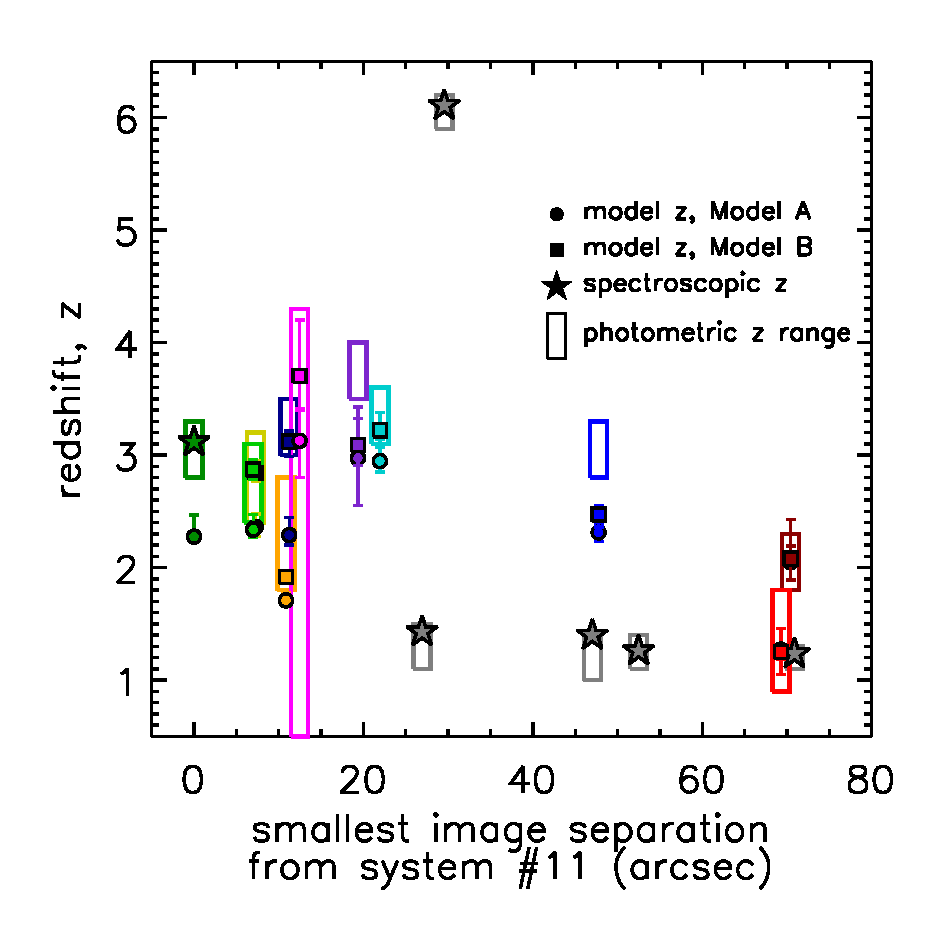
\includegraphics[width=\textwidth]{Chap2/c2f7.eps}
\caption[Model-predicted redshifts vs. spectroscopic redshifts for preliminary and submitted lens models of Abell S1063]{We show the model-predicted redshifts of image systems included as constraints in our preliminary lens model (Model A in text, circles) of Abell S1063 and the model we present here (Model B in text, squares) plotted versus their shortest image plane separation from one of the images in system \#11. The gray stars indicate image systems fixed to their spectroscopic redshifts in both models. In Model A, the redshift of image system \#11 is left as a free parameter, where in model B, we fix the redshift to the spectroscopic redshift. There is a systematic increase in the model-predicted redshifts from Model A to Model B for the images closest ($<50"$) to the new spectroscopic redshift system \#11. We also plot the 95\% confidence range for photometric redshifts.}
\label{chap2:fig:as1063_free_z_dist}
\end{figure}

\begin{figure}[h]
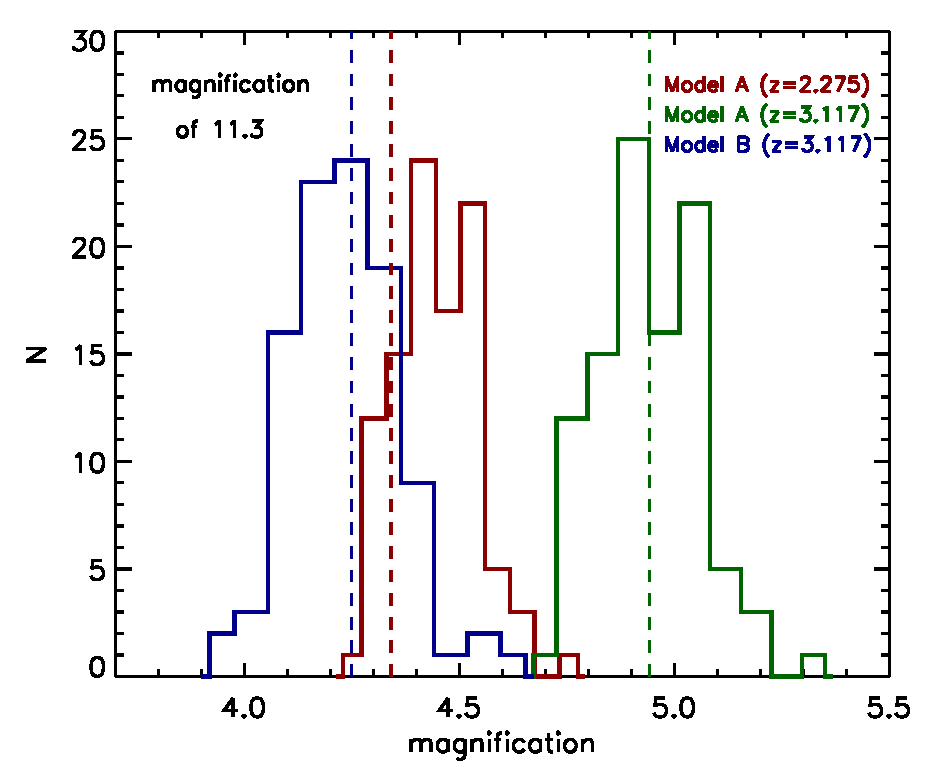
\includegraphics[width=\textwidth]{Chap2/c2f8.eps}
\caption[Magnifications of image \#11.3 in Abell S1063 for Model A and Model B]{We plot the magnifications of image \#11.3 from Model A (the redshift of image system \#11 is a free parameter in the model) and Model B (the redshift of image \#11 is fixed to the spectroscopic redshift). For Model A, we derive the magnification for two source plane redshifts: the model-predicted redshift of the image system $z=2.275$ (red) and the spectroscopic redshift $z=3.117$ (green). Model B (blue) is set to the spectroscopic redshift. The dashed lines represent the value of magnification of the best-fit model.}
\label{chap2:fig:mag11}
\end{figure}

\subsection{The cumulative magnification power of the HFF}
The derivation of detailed magnification maps, as presented in this work, enable the use the HFF clusters as cosmic telescopes to study the background Universe; in particular, one of the science goals of the HFF is to study the galaxy population at $z\sim9$.  The lensing magnification simultaneously acts to produce two competing effects: it increases the observed source-plane area, and it magnifies faint source above the detection limit. In a given solid angle on the sky the former effect reduces the number of bright galaxies, and the latter increases the number of faint galaxies. It is thus constructive to estimate the source-plane area (and co-moving volume) that is magnified by the cluster as a function of magnification factor. 

In Figure~\ref{chap2:fig:volumes} we plot the magnification power of each cluster, as the cumulative volume and area magnified above a certain value as a function of magnification. For each cluster field, the source-plane area is computed by de-lensing the $z=9$ magnification map to the source plane, and summing the area that is magnified by more than a given magnification. For the purpose of estimating the volume we multiply this area by the co-moving distance between $z=8.5$ and $z=9.5$. We find that on average, the total $z=9$ area that is observed through each cosmic telescopes is about 20\% of the WFC3/IR field of view. However, 10\% of this area is magnified by more than a factor of 6, which is equivalent to having a limiting magnitude at least 2 magnitudes fainter in these areas.

\begin{figure}[t]
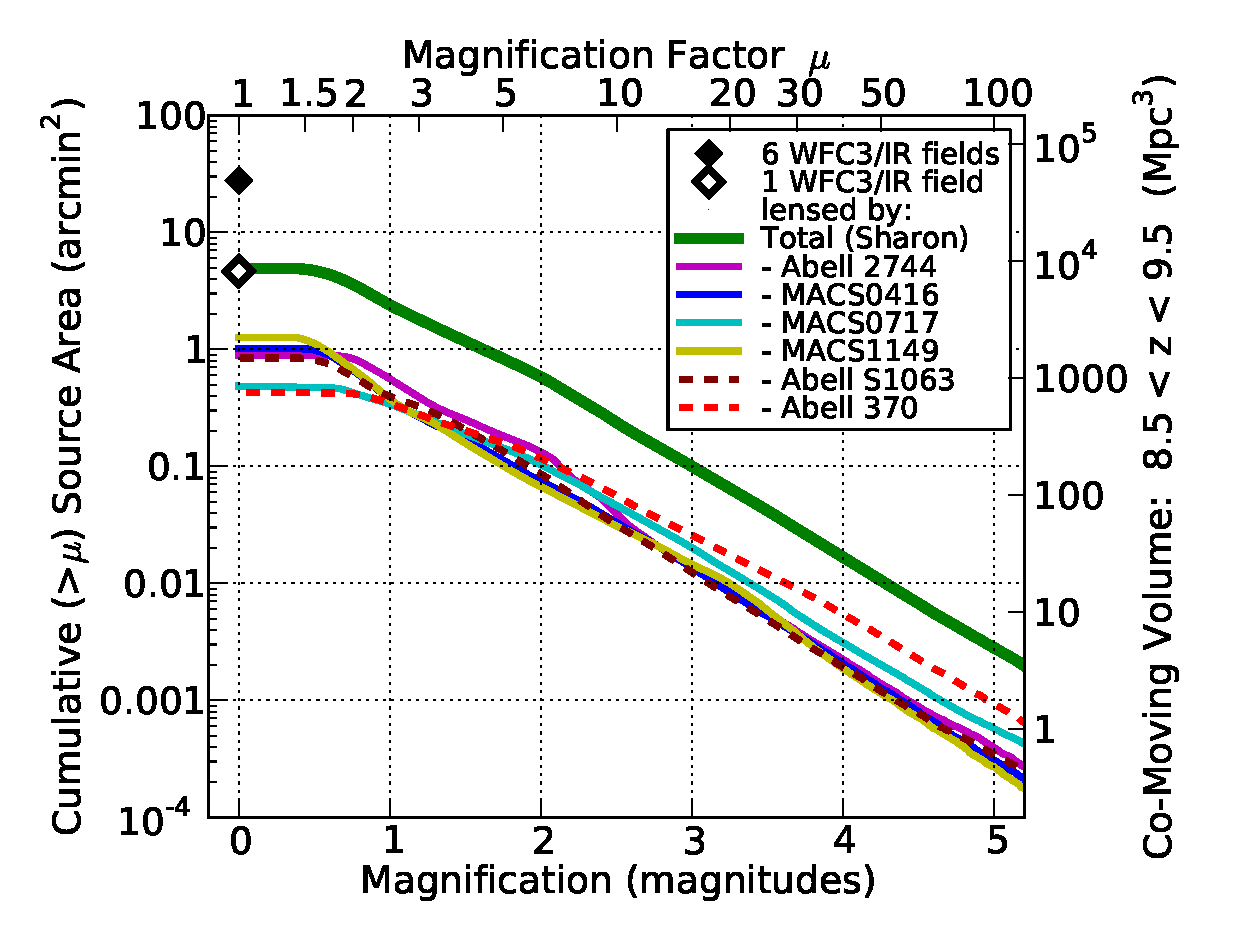
\includegraphics[width=\textwidth]{Chap2/c2f9.eps}
\caption[Cumulative area and co-moving volume of $z\sim$9 background sources lensed by each of the HFF clusters]{We show the cumulative area and co-moving volume of background sources at $8.5<z<9.5$ lensed by each of the HFF clusters to magnification $\mu$ and higher. We show, for reference, the corresponding area and co-moving volume of a one and six WFC3/IR FOVs (diamonds).}
\label{chap2:fig:volumes}
\end{figure}

\subsection{Model comparisons}

The coordinated parallel effort to generate multiple independent lens models for the HFF provide a unique opportunity for the lensing community to analyze in depth for the first time the systematics of various lens modeling techniques. \hst\ imaging continues to be key for developing methods for lens modeling in clusters, as the pristine image quality is crucial for the identification of multiple image systems for strong lensing and for accurately determining the shear fields for weak lensing. 

Within the past decade or so, we have seen the development of several innovative computational softwares for lens modeling (e.g., \texttt{LENSTOOL}, \citet{Jullo:2007lr}; \texttt{LensPerfect}, \citet{Coe:2008mz}; \texttt{glafic}, \citet{Oguri:2010gr}; \texttt{GRALE}, \citet{Liesenborgs:2010gf}; strong and weak lensing united, \citet{Bradac:2005ve}; SaWLens, \citet{Merten:2009ul}; light-traces-mass, \citet{Broadhurst:2005qy} and \citet{Zitrin:2009qf}; \texttt{GRAVLENS}, \citet{Keeton:2001lr}). Indirect comparisons exist in the literature when different methods were applied to the same clusters; however, direct comparisons of the models require similar modeling inputs and quantitative comparisons are few in number. In-depth analyses of the systematic errors of different lens modeling methods have yet to be done.

The five lens modeling teams for the preliminary HFF lensing maps each use unique modeling techniques, which include strong and weak lensing approaches, parametric and non-parametric constructions of the lensing potential, and differing assumptions regarding the shapes of individual mass halos to list only a few of the differences. The HFF models are perfect for model comparisons since the modeling inputs are nearly identical due of the collective agreements amongst the modeling teams to share these inputs (i.e. photometric and spectroscopic redshifts, galaxy catalogs, etc.) amongst each other. The lens modeling techniques used to map the HFF clusters will be compared directly through the lens modeling of simulated clusters prepared in a similar manner as \citet{Meneghetti:2008oz} and designed to represent the depth and image quality of a complete HFF data set. These model comparisons are ongoing and will be presented elsewhere.

\subsection{Model revisions}

As more data on the HFF clusters becomes available, the strong lensing models will be iterated on and improved. Preliminary models can be used to hunt for more multiple image systems in the deeper data sets. Ground-based campaigns are ongoing to obtain more spectroscopic redshifts to improve the precision of these models.

Future models could incorporate more free parameters to account for both visible and unseen structure along the line of sight. As is indicated in Table \ref{chap2:tab:model_summary}, all of these lens models are over-constrained, a trend which will continue as more image systems are discovered, allowing for more free parameters to be added to the models. Currently our models account for structure only at the cluster redshift (correlated) with a few exceptions in some of our models for obvious foreground interlopers, though other uncorrelated groups and cosmic variance could also contribute to the lensing. \citet{Bayliss:2014fk} show from spectroscopic observations evidence for large scale uncorrelated substructure along the line of sight to strong lensing clusters, which could become a significant systematic in lens modeling precision, and \citet{DAloisio:2013ul} estimate that such structures could account for fluctuations of $\sim30\%$ in magnification for highly-magnified sources ($\times10$). As we noted in \S \ref{chap2:sec:results_a2744}, there is clear evidence in some of the clusters that line-of-sight structure plays significant role in the overall lensing potential. These clusters would be ideal for developing and testing multi-plane lens modeling technique on observational data. 

\section{Summary}
\label{chap2:sec:conclusion}

We present high-quality strong lens models for each of the six Frontier Fields clusters. The models are based on archival \hst\ imaging, obtained prior to the deep HFF imaging in Cycle 21, and on ground-based spectroscopy of the lensed galaxies and cluster members, including the new spectroscopic redshifts for lensed galaxies in Abell S1063 and Abell 2744 we present in this work. We compute parametric, strong-lensing models for each cluster in the HFF using the systems of multiply imaged background galaxies as constraints. The HFF clusters are powerful gravitational lenses; we quantify from our lens models their cumulative magnification power of high redshift galaxies. We compare the cluster masses computed from our models to other lens models in the literature. We generally find that the early models, that did not use redshifts as inputs, are in disagreement with our results, and typically produce 10-20\% higher mass at the core of the cluster. The models presented in this work are publicly available for use in analyzing the lensing of the high-redshift Universe behind these galaxy clusters. We outline the formalism for how the outputs of our lens models can be used to derive the magnifications of any background source in the entire FOV of the HFF observations, and discuss the caveats of using our lens models in these analyses. Specifically, we note that the regions of highest-precision magnification values are those that lie closest to the image constraints used in the model. The highest statistical uncertainties in magnification values lie close to critical curves, where the gradient in magnification is high, and more than $\gtrsim1'$ from the strong-lensing region, where there are no strong lensing constraints. We begin to address systematic uncertainties in lens modeling, noting that the derived models can change significantly when the assumptions regarding the redshifts of multiply imaged background galaxies are different and plan to investigate these systematics more thoroughly in the future. As more data become available for each cluster as the \hst\ observations take place over the next three years, we will revise these models and provide the public with the most precise models possible. These revisions will be based on new image systems of lensed background galaxies, better constraints on photometric redshift priors, new spectroscopic confirmation of the lensed arcs from ground-based observatories, incorporating line of sight structure, and new inquiry into the systematic modeling errors, which will unfold after ongoing model comparisons.

\vspace{24pt}

Some of the data presented in this paper were obtained from the Mikulski Archive for Space Telescopes (MAST). STScI is operated by the Association of Universities for Research in Astronomy, Inc., under NASA contract NAS5-26555. Support for MAST for non-HST data is provided by the NASA Office of Space Science via grant NNX13AC07G and by other grants and contracts. This work was supported by NASA Grant \#5-26555. KS acknowledges support from the University of Michigan's President's Postdoctoral Fellowship.

We thank the anonymous referee for contributing helpful comments and feedback. We would like to thank the Frontier Fields lens modeling teams for sharing unpublished data (image identifications, photometric and spectroscopic redshift measurements, galaxy catalogs, and ground-based imaging) which we used as inputs to our lens models and useful for discussion. We thank Marceau Limousin for generously providing the catalogs of galaxy cluster members for \MACSzeroseven\ and \MACSeleven. For their help with supplementary data that were used to guide our mask design for Abell S1063, we wish to thank Daniel Gruen, Piero Rosati, and Stella Seitz). We also thank Daniel Gruen for providing the aperture masses from weak lensing models for direct comparisons with the models presented in this paper. We thank Daniel Gifford for carrying out our November 2013 Magellan/IMACS observations of Abell 2744.



 
\chapter{The systematics of strong lens modeling quantified: the effects of constraint selection and redshift information on magnification, mass, and multiple image predictability}
\label{chap:ares_systematics}
\section{Preface}

This works has been partially adapted from published work in the Astrophysical Journal, Volume 832, page 82 \citep{Johnson:2016rt}, with co-author Keren Sharon. The paper is adapted and partially reproduced here under the non-exclusive rights of republication granted by the American Astronomical Society to the paper authors.

For my part of this project, I created the fiducial model of ARES and all of the 300+ test models used to evaluate the systematic errors. I wrote nearly all of the text and created all of the figures.

\section{Abstract}
Until now, systematic errors in strong gravitational lens modeling have been acknowledged but have never been fully quantified. Here, we launch an investigation into  the systematics induced by constraint selection. We model the simulated cluster Ares 362 times using random selections of image systems with and without spectroscopic redshifts and quantify the systematics using several diagnostics: image predictability, accuracy of model-predicted redshifts, enclosed mass, and magnification. We find that for models with $>15$ image systems, the image plane rms does not decrease significantly when more systems are added; however, the rms values quoted in the literature may be misleading as to the ability of a model to predict new multiple images. The mass is well constrained near the Einstein radius in all cases, and systematic error drops to $<2\%$ for models using $>10$ image systems. Magnification errors are smallest along the straight portions of the critical curve, and the value of the magnification is systematically lower near curved portions. For $>15$ systems, the systematic error on magnification is $\sim2\%$. We report no trend in magnification error with fraction of spectroscopic image systems when selecting constraints at random; however, when using the same selection of constraints, increasing this fraction up to $\sim0.5$ will increase model accuracy. The results suggest that the selection of constraints, rather than quantity alone, determines the accuracy of the magnification. We note that spectroscopic follow-up of at least a few image systems is crucial because as models without any spectroscopic redshifts are inaccurate across all of our diagnostics.

%==================================================================================
%   INTRODUCTION
%==================================================================================
\section{Introduction}
\label{chap3:sec:introduction}

Since the discovery of the first gravitationally lensed arc in the field of cluster Abell 370 nearly three decades ago \citep{Soucail:1988kx}, astronomers have been taking advantage of the lensing magnification boost from massive galaxy clusters to observe the distant Universe. Gravitational lensing has the advantage of achromaticity, making spectral observations of these lensed objects comparable to unlensed sources in the field. Additionally, the strong lensing evidence traces the total mass distribution of the cluster, allowing for accurate reconstructions of the projected mass density of clusters, especially on small scales ($<100$ kpc) where other mass tracing methods are sensitive, yet lack the resolution of strong lensing. Lensing is sensitive only to mass and not to gas physics that can contribute to the uncertainties of mass scaling relations where the observable depends on the state of the hot intercluster medium.

However, one of the largest challenges in exploiting gravitational lensing remains in calibrating these ``cosmic telescopes". Both strong and weak lensing methods have been used extensively to measure the mass distribution of galaxy clusters. Numerous weak lensing surveys have allowed for a deep investigation into the statistical and systematic errors of weak lensing methods \citep{Shirasaki:2014qf,Applegate:2014jk,Massey:2013xy}. Similar analyses for strong lensing have lagged behind those of weak lensing for two main reasons: (1) accurate strong lens models require an exquisite image quality to robustly identify multiple images \citep{Kneib:1996kb}, and (2) the occurrence of strong lensing events is lower than weak lensing, making it more difficult to find strong lensing clusters to model. The {\it Hubble Space Telescope} (\hst) has been the primary workhorse for strong lensing observations since the installation of WFPC2. The probability of finding strong lenses is indeed small \citep{Wambsganss:2004vn,Bartelmann:1998fr}; but as predicted, several hundred strong lensing clusters have been found directly in several optical surveys \citep{Hennawi:2008mz,Gladders:2003zr} and after optical follow-up of clusters found in Xray-selected \citep{Postman:2012lr} and Sunaev-Zel'dovich effect-selected clusters \citep{Bleem:2015gf,Menanteau:2010fu}. Strong lensing mass estimates of the cores of these clusters when combined with other proxies for mass at larger scales will allow for measurements of the mass-concentration relation of galaxy clusters \citep{Merten:2015rz,Oguri:2012bs,Gralla:2011kx} across a range of cluster masses and redshifts. These strong lensing clusters highly-magnify numerous galaxies from the peak of cosmic star formation density around $z=2$ \citep{Bayliss:2011gf}, allowing for zoomed-in studies of star formation at a time when the Universe produced most of its stars \citep{Madau:2014qd}. Currently, strong lensing clusters are our best chance of finding the most distant galaxies at $z>8$, which may be responsible for re-ionizing the universe \citep[][to name a few]{McLeod:2015nr,Atek:2015qv,Zitrin:2014uq,Coe:2015qf}. With the ever increasing number of known strong lenses it will be important to fully understand how well we can quantify both the statistical and systematic errors in modeling strong lensing galaxy clusters.

Estimating the {\it statistical} errors in strong lens modeling has become nearly routine with the advancement in lens modeling codes to utilize Markov Chain Monte Carlo (MCMC) algorithms to adequately explore parameter spaces. The literature only mentions instances where systematic errors have been revealed between different models of the same cluster or when comparing new models of a cluster to earlier and obsolete models. For example, \citet{Smith:2009lr} found that including redshift information of the strong lensing constraints has a significant effect in constraining the slope of the mass distribution. Similarly, \citet{Johnson:2014tg} found that the magnification can vary beyond the statistical errors when the redshift information is added for a single system. \citet{Jauzac:2015xy} report an overall increase in magnification values for their new model of Abell 2744 using full-depth Hubble Frontier Fields (HFF) data; this effect has many possible causes: adding dozens of new image systems as constraints, including new spectroscopic redshifts, and/or correcting a misidentified image system.

\begin{figure*}
\center
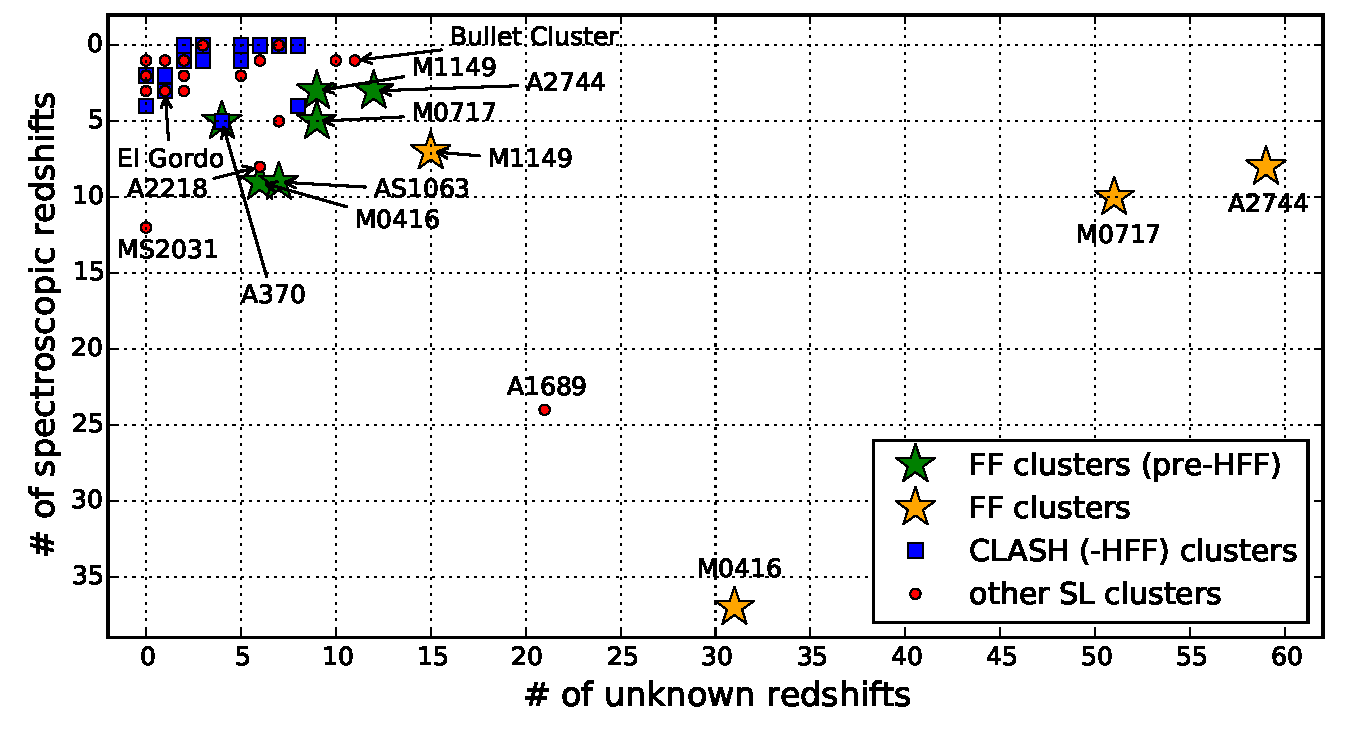
\includegraphics[width=\textwidth]{Chap3/c3f1.pdf}
\caption[Strong lensing models from the literature]{The distribution of cluster strong lensing models from the literature, separated into number of strong lensing image systems with spectroscopic redshifts and those with unknown redshifts. The green stars represent the status of the HFF cluster lens models prior to HFF observations \citep{Johnson:2014tg,Richard:2014gf}, while the yellow stars show the most complete lens models to date on clusters with full HFF data \citep{Caminha:2017rw,Limousin:2016ty,Kawamata:2016nr,Treu:2016lr,Jauzac:2016dn,Jauzac:2014qd,Jauzac:2015xy}. We also include several other clusters from the literature, including those from the CLASH survey that do not overlap with the HFF clusters \citep{Zitrin:2015lq}. Other clusters include well-known lensing clusters such as Abell 1689 \citep{Diego:2015tg}, the Bullet Cluster \citep{Bradac:2009qd}, El Gordo \citep{Zitrin:2013hl}, Abell 1703 \citep{Limousin:2008lr}, Abell 2218 \citep{Eliasdottir:2007ve}, and many others \citep{Sharon:2015xe,Richard:2015lr,Richard:2010zp,Richard:2007rr,Sharon:2014fj,Bayliss:2014lr,Sharon:2012ly,Zitrin:2011qy}.}
\label{chap3:fig:slclusters}
\end{figure*}

While it is true that each individual method has its own systematic errors, all modeling methods are subject to errors due to the availability of constraints. The HFF clusters and Abell 1689, with a wealth of deep multi-wavelength imaging and spectroscopy, have unprecedented numbers of image systems identified and have some of the most precise lens models of clusters in existence \citep{Kawamata:2016nr,Treu:2016lr,Jauzac:2016dn,Diego:2015tg,Jauzac:2015xy,Jauzac:2014qd}. Yet, these clusters are seven unique lensing sight lines; in fact, most clusters only have a handful of multiple images (see Figure~\ref{chap3:fig:slclusters}). This reality stems from a few factors: (1) the aforementioned clusters are some of the most massive clusters, many showing signs of ongoing growth through mergers \citep{Jauzac:2015qf,Merten:2011fk}, resulting in larger lensing cross-sections, (2) have some of the deepest \hst\ data allowing for identification of fainter multiple image systems, and (3) have extensive spectroscopic campaigns which allow for the redshift confirmation of multiple image systems. Determining to what degree systematic errors are induced upon a lens model due to the availability of constraints is a high priority, especially for lower mass clusters which tend to lens fewer multiple image systems or massive clusters with shallow observations.

In this paper we begin to address several questions surrounding the topic of systematic errors in lens modeling. How does changing the number of constraining multiple image systems in a lens model affect the accuracy of strong lens models? Similarly, how does increasing the number of spectroscopic redshifts influence a model's accuracy? These questions are timely in this new era of strong lensing where high quality data are allowing for the most precise (i.e., low statistical uncertainty) models with high numbers of identified lensing constraints. Answering these questions will help guide the lensing community's focus to improve the quality of future strong lensing models. Spectroscopic campaigns are expensive: lensed galaxies, while magnified, are still faint and require long integrations on large telescopes, thus, we must determine their necessity for strong lens modeling. We show that it is critical for strong lens models to have at least a few spectroscopically-confirmed redshifts of image systems to dramatically reduce systematic errors.

This paper is organized as follows. We begin with a description of the experimental design in \S\ref{chap3:sec:experimental_design}. We describe the fiducial lens model in \S\ref{chap3:sec:lens_model} used for our analysis. In \S\ref{chap3:sec:methods} we describe our methodology for quantifying lens modeling systematics and report the results in \S\ref{chap3:sec:results}. Finally we summarize our work in \S\ref{chap3:sec:discussion} and discuss plans for future work in \S\ref{chap3:sec:future}. We assume a \LCDM\ universe with $\Omega_M=0.3$, $\Omega_\Lambda=0.7$, and $H_0=70\ \mathrm{km\ s^{-1}\ Mpc^{-1}}$. This cosmology yields an angular-physical scale of $1"=6.104$ kpc to the Ares cluster redshift $z=0.5$.


%==================================================================================
%  EXPERIMENTAL DESIGN
%==================================================================================
\section{Experimental Design}
\label{chap3:sec:experimental_design}
The goal of this study is to investigate quantitatively how the selection of strong lensing constraints, i.e., the redshifts and multiple images of strongly-lensed galaxies, affect lens models. We do this by generating 350 test models of the same gravitational lens, each test model uses a different random subset of the available constraints. The results of the test models are compared to a fiducial model that uses the full set of constraints as input. In this section we briefly describe our choices, while a thorough discussion is given in the following sections. 

The best-case-scenario fiducial model is a lens model of the simulated cluster Ares, a model that was initially computed for the purpose of the lens modeling comparison challenge \citep{Meneghetti:2016xe}. The fiducial model is constrained by 66 lensed galaxies with known redshifts. All test models will be compared to this fiducial model, which uses all lensing constraints and the true redshifts of the sources.

The parameter space that is covered by the test models is the number of lensed galaxies with spectroscopic redshifts, and the number of lensed galaxies without spectroscopic redshifts that are used to constrain the model. Each of those parameters is varied between zero and 25. For each combination of parameters we generate 10 models, with different galaxies selected randomly as constraints in each one. The tested combinations of number of lensing constraints with and without spectroscopic redshifts  cover scenarios similar to the HFF clusters, including early pre-HFF models with small number of constraints and as low as three spectroscopic redshifts, to the richest post-HFF datasets with hundreds of multiple images and dozens of new spectroscopic redshifts. 

We compare the test models on a few metrics: image plane rms as a measure of predictability of multiple images, model-predicted redshifts of systems without spectroscopic redshifts, mass distribution, and magnification. The results are compared with the fiducial model, rather than the simulation, in order to separate the systematic error induced by the constraints from other potential sources of systematics. The systematic error between the fiducial model and simulation truth may be sensitive to the exact modeling algorithm and parameterization choice, which is beyond the scope of this paper, yet will be important to investigate. We refer the reader to \citet{Meneghetti:2016xe} for current work, comparing different lensing methods. 

While we are only investigating this effect on a single method, this study is applicable to all strong lensing methods. Despite the variety of lensing methods (i.e., parametric versus non-parametric, see below), all methods are using the same lensing evidence to infer the mass distribution. 

%==================================================================================
%  STRONG LENS MODELING
%==================================================================================
%\section{Strong lens modeling}
%\label{chap3:sec:slmodeling}
%
%While diverse in computational algorithms, all strong gravitational lens modeling codes have a common goal: solve the lens equation 
%
%\begin{equation}
%\beta_{ij} = \theta_{ij} - \alpha_{ij}
%\end{equation}
%
%\noindent for the image plane positions $\theta_{ij}$ of each multiply imaged background source that map to location $\beta_{ij}$ in the source plane. The solution is the deflection field tensor $\alpha_{ij}$, which can be differentiated to solve for the projected surface mass density $\Sigma$,
%
%\begin{equation}
%\nabla_{ij}\alpha_{ij} = \frac{4\pi G}{c^2}\frac{\dls(\zl,\zs)}{\ds(\zs)} \dl(\zl)\ \Sigma,
%\label{eqn:SMD}
%\end{equation}
%
%\noindent where $\ds$, $\dl$, and $\dls$ are the angular diameter distances between the observer and the source at redshift $\zs$, between the observer and the lens at redshift $\zl$, and between the lens and source, respectively. When the lensing mass is contained to a single plane at $\zl$, then the deflection angle scales only with the lensing fraction
%
%\begin{equation}
%\frac{\dls}{\ds}(\zs) = \frac{\alpha_{ij}(\zs)}{\alpha_{ij}(z\rightarrow\infty)},
%\label{eqn:dlsds}
%\end{equation}
%
%\noindent which is a function of a single variable $\zs$. Thus, it is clear that both the image plane position $\theta_{ij}$ and the source redshift $\zs$ are needed to determine the full three-dimensional lensing geometry needed to constrain $\Sigma$.
%
%Strong lens modeling can include other observable strong lensing effects that constrain other first- and second-order derivatives of the lensing potential, including time delays, magnification ratios between different images of the same source, and flexion (distortion of the background source). These methods can be implemented in lens modeling codes, but are more prone to systematic error from the uncertainty of the observations themselves (i.e., lack of measured time delays, microlensing effects on magnification ratios, need for high-quality imaging for shape measurements). Measuring a centroid of an image of a lensed galaxy is straight-forward and typically the error in position is smaller than the errors in lensing due to cosmic variance and structure along the line of sight \citep{Limousin:2007fk}.
%
%There are generally two schools of thought for lens modeling codes: parametric and non-parametric methods. Parametric methods (e.g., Lenstool, \citealp{Jullo:2007lr}; glafic, \citealp{Oguri:2010gr}; gravlens, \citealp{Keeton:2001lr}; light-traces-mass, \citealp{Broadhurst:2005qy} and \citealp{Zitrin:2009qf}; GLEE, \citealp{Suyu:2012qf,Suyu:2010xy}) assume that the lensing potential and mass distribution of the lens can be expressed as a superposition of parameterized density distributions, and those parameters can be solved from the lensing evidence.  A common assumption for these models is that mass distribution follows that of the light (i.e., cluster member galaxies are assigned their own halos), however, this assumption can be applied more rigorously or loosely depending on the method. Non-parametric methods (e.g., SWunited, \citealp{Bradac:2008kx}; SaW lens, \citealp{Merten:2011fk}; LensPerfect, \citealp{Coe:2008mz}; WSLAP, \citealp{Diego:2007qf,Diego:2005ye}; Grale, \citealp{Liesenborgs:2010gf}) make no assumptions about the mass distribution and instead solve for each ``pixel" in the surface mass density of an adaptive grid with higher resolution near the constraints and peak of the density distribution. Some codes have been hybridized to include aspects of both parametric and non-parametric techniques \citep[ex., ][]{Jullo:2009ij}.

%==================================================================================
%   THE FIDUCIAL LENS MODEL
%==================================================================================
\section{The fiducial lens model}
\label{chap3:sec:lens_model}

\subsection{The simulated cluster Ares}
\label{chap3:sec:ares}

\begin{figure*}
\center
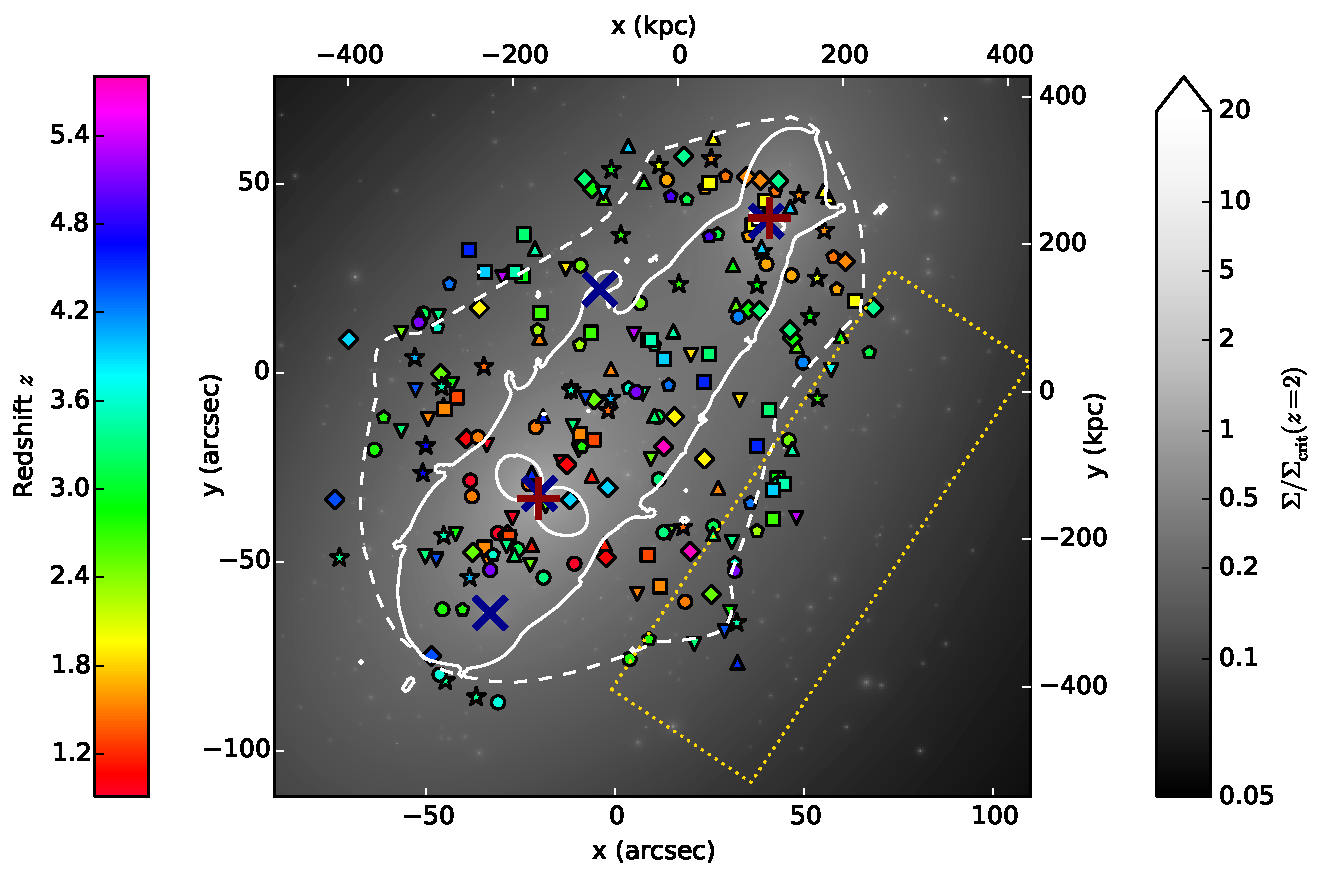
\includegraphics[width=0.9\textwidth]{Chap3/c3f2.pdf}
\caption[Surface mass density of Ares fiducial lens model]{The fiducial lens model of Ares. The grayscale image shows the projected surface mass density $\Sigma$ in units of the critical density $\Sigma_\mathrm{crit}=(c^2 \ds)/(4\pi G \dls \dl)$ at $z=2$. The locations of the multiple images used in the lens model are shown by the symbols, with colors indicating redshift. Images that match to the same source have the same redshift and are represented by the same symbol. The $z=2$ critical curve is shown by the solid white lines. The dashed white lines indicates the region where the model predicts multiple images for $z=2$. The red crosses and blue x's mark the centers of the two cluster halos and four galaxy halos listed in Table~\ref{chap3:tab:params}, respectively. The gold dotted boxed region indicates the pixels used to generate the plots in Figures~ \ref{chap3:fig:histograms},  \ref{chap3:fig:specz_fraction}, \&  \ref{chap3:fig:single_compare}.}
\label{chap3:fig:hst}
\end{figure*}

A full description of the Ares simulated cluster is given in \citet{Meneghetti:2016xe}. In short, the Ares cluster simulation is designed to mimic a massive cluster that is an efficient gravitational lens. The publicly available software MOKA \citep{Giocoli:2012lr} is used to create simulated lensing signals from clusters, including a number of scaling relations derived from N-body simulations, a mass-concentration relation, a subhalo mass function, and subhalo tidal stripping effects on truncation radii. The main cluster potential is composed of two triaxial clumps with masses $1.8\times10^{15}\ \mathrm{M_\odot}$ and $1.3\times10^{15}\ \mathrm{M_\odot}$ following the Navarro-Frenk-White profile \citep[NFW;][]{Navarro:1997qa}, separated by $\sim570$ kpc, along with two central cluster galaxies near the centers of these gravitational wells, which are modeled by triaxial profiles. The galaxy-scale halos are modeled as singular isothermal spheres.

The baryonic component of Ares follows a halo-occupation distribution (HOD) technique, where it is assumed that the stellar mass of a galaxy is tightly correlated with the depth of the gravitational potential well that it occupies. The B band luminosities are assigned to each halo by MOKA using the relations described in \citet{Giocoli:2012lr}, which follow closely with the results by \cite{Wang:2006kk}. Then, a spectral energy distribution is assigned to each galaxy based on this luminosity and
empirical relations such as the morphology-density relation and the fraction of morphological types observed in clusters as a function of radius. Foreground galaxies and stars are added to the imaging; however, there is no additional mass along the line of sight to the cluster associated with these interlopers.

To simulate the lensed background Universe, the lensing signal from the cluster Ares is input into SkyLens \citep{Meneghetti:2010mi,Meneghetti:2008oz}, which ray traces real galaxies from the Hubble Ultra Deep Field \citep{Beckwith:2006rt} to the image plane. SkyLens creates mock \hst\ imaging of the results, which match the depth and wavelength coverage of the HFF observations.

The primary utility of Ares is for the on-going HFF lens modeling comparison study \citep{Meneghetti:2016xe}. The same teams that modeled the HFF clusters, using different methods, were invited to compute lens models for Ares. Each team was given the simulated imaging along with a catalog of all the multiple image systems and redshifts, but were initially blind to the true mass distribution. The goal of this study is to identify how different methods reproduce the true mass and magnification of a HFF-like cluster when given identical inputs and to identify systematic errors across lens models that can be addressed when creating the best lens models. The initial ``blind" modeling took place mid-2014, after which the mass and magnification were unveiled to the modeling teams. Our goals in this work can be thought of the tangent of those for the comparison study: rather than determine the systematics for different modeling methods using identical inputs, we are testing with a single method how varying the quantity and redshift information of constraints induces systematic errors.

\subsection{The lens model}
\label{chap3:subsec:fiducial_model}

We follow a similar methodology for modeling Ares as \citet[Chapter 2]{Johnson:2014tg}. We use the publicly-available parametric modeling software Lenstool \citep{Jullo:2007lr}, which utilizes a Bayesian MCMC to explore the parameter space of the lensing distribution. We construct a lens model using all of the available lensing evidence that accurately reproduces the simulation mass and magnification. We refer to this model as the fiducial model, representing the best possible model we can create with our methods when all of the information (images, redshifts, mass distribution, etc.) is revealed. The fiducial model critical curves and images are shown in Figure~\ref{chap3:fig:hst}.


\begin{deluxetable}{cccccccc}
\tablecolumns{8}
\tabletypesize{\scriptsize}
\tablewidth{0pt}
\tablecaption{List of fiducial lens model constraints}
\tablehead{\colhead{} & \colhead{$x$ (")} & \colhead{$y$ (")} & \colhead{$e$} & \colhead{$\theta$ ($^\circ$)} & \colhead{$r_\mathrm{core}$ (kpc)} & \colhead{$r_\mathrm{cut}$ (kpc)} & \colhead{$\sigma_0$ ($\mathrm{km\ s^{-1}}$)}}
\startdata
cluster halo \#1 & $-20.3^{+0.1}_{-0.2}$ & $-33.3^{+0.1}_{-0.3}$ & $0.510^{+0.003}_{-0.016}$ & $50^\pm0.5$ & $100^{+3}_{-2}$ & [1500] & $1250^{+5}_{-7}$ \\[5pt]
cluster halo \#2 & $40.8^{+0.1}_{-0.3}$ & $40.9^{+0.4}_{-0.2}$ & $0.54^{+0.00}_{-0.05}$ & $74^{+1}_{-2}$ & $56\pm3$ & [1500] & $765^{+9}_{-5}$ \\[5pt]
galaxy halo \#1 & [-33.0] & [-63.6] & [0] & \nodata & [0] & $90^{+70}_{-0}$ & $240^{+130}_{-0}$ \\[5pt]
galaxy halo \#2 & [-20.0] & [-32] & $0.13^{+0.03}_{-0.07}$ & $156^{+27}_{-6}$ & [0] & [1500] & $502^{+10}_{-5}$ \\[5pt]
galaxy halo \#3 & [40.0] & [40.0] & $0.77^{+0.04}_{-0.20}$ & $5^{+5}_{-6}$ & [0] & [1500] & $290^{+6}_{-29}$ \\[5pt]
galaxy halo \#4 & [-4.0] & [22.0] & [0] & \nodata & [0] & [1500] & $213^{+4}_{-11}$ \\[5pt]
\hline \\[-5pt]
$L^\star$ galaxy & \multicolumn{4}{c}{$m_\star=20.00,\ z=0.5$ (ACS F606W)} & 0 & 20 & 100
\enddata
\vspace{-20pt}
\tablecomments{The ellipticity is defined as $e=(a^2-b^2)/(a^2+b^2)$, where $a$ and $b$ are the semimajor and semiminor axes, respectively. The position angle is measure counterclockwise from the $+x$ axis. Parameters in square brackets are not optimized in the model. Errors represent the $1\sigma$ spread in values from the MCMC.}
\label{chap3:tab:params}
\end{deluxetable}


The mass distribution is parameterized by pseudo-isothermal elliptical mass distributions \citep[PIEMD or dPIE; ][]{Limousin:2005cr}; the profile is described by a fiducial velocity dispersion $\sigma_0$ to normalize the potential, an ellipticity and position angle, and core radius $r_\mathrm{core}$ and cut radius $r_\mathrm{cut}$ which control the inner and outer slopes of the profile, respectively. A summary of those halo parameters are given in Table \ref{chap3:tab:params}. We use two halos to represent the dark matter cores in the cluster, which were also included in our ``blind" lens model. We include the masses of galaxy cluster members as small perturbers to the smooth dark matter potential of the cluster. The galaxies are selected by red-sequence membership and their halo parameters are scaled by their brightness following

\begin{eqnarray}
\sigma_0&=& \sigma_0^\star \left(\frac{L}{L^\star}\right)^{1/4}, \nonumber \\
r_\mathrm{core} &=& 0 \\
r_\mathrm{cut} &=& r_\mathrm{cut}^\star \left(\frac{L}{L^\star}\right)^{1/2} \nonumber
\end{eqnarray}

\noindent where $\sigma_0^\star, r_\mathrm{core}^\star, r_\mathrm{cut}^\star$ are the parameters of an $L^\star$ galaxy at the simulated cluster redshift $z=0.5$. For four cluster galaxies (including the two brightest galaxies in both cores), we allow some of the parameters to deviate from the scaling relations and be guided by the lensing of nearby multiple images, as we routinely do in lens models of real clusters. Galaxy halo \#1 (as indicated in Table \ref{chap3:tab:params}) is a massive galaxy that has a significant impact on the location of the critical curve in the southwestern portion of the image plane. Galaxy halos \#2 and \#3 lie near the centers of the two massive cluster halos and thus have an impact on the locations of the radial arcs across the entire cluster. The fourth galaxy halo is massive enough to produce its own protrusion of the tangential critical curve created by the two massive cluster halos, thus influencing the lensing of several nearby images. These four galaxies are needed for models with many constraints; however, their parameters are more difficult to constrain in the case when there are no images within a few arcseconds of the halo.

Our treatment of the scaling relations for Ares deviate from those of the models in \citet{Johnson:2014tg} due to the construction of the simulation. We did not include shape information from the light distribution to guide the galaxy shapes in the lens model and instead modeled the halos as single isothermal spheres ($\mathrm{ellipticity} = 0$, $r_\mathrm{core} = 0$) as to match closely to the parameterization of the simulation. We ran a simple optimization to explore which scaling parameters produce a close match between the simulated halos and lens model halos. All three of these parameters are highly degenerate when determining the mass of a halo and thus no single parameter combination was determined to be a significantly better fit over others. Additionally, the typical scale of $r_\mathrm{cut}$ is several tens to a hundred kiloparsecs; at this scale the halo of a galaxy begins to overlap with neighboring galaxies and the main cluster potential starts to dominate the local surface mass density. Thus, $r_\mathrm{cut}$ is difficult to constrain. We selected a parameter combination that was reasonable with those of previous strong lensing models and matched well with the simulation: $\sigma_0^\star=100\ \mathrm{km\ s^{-1}}$, $r_\mathrm{cut} = 20$ kpc, and $m_\mathrm{F606W}^\star=20.0$. Due to a different choice of scaling relations and photometric band used for scaling, we do not expect the simulation and lens model to match perfectly. Our goal with this optimization is to minimize the effects of scaling parameter selection on the overall systematic errors of the lens model we are attempting to measure. The mass of the fiducial model is reconstructed with an accuracy of $-0.24^{+0.23}_{-0.30}\%$ of the simulation mass within 500 kpc of the cluster center.

A list of simulated multiple images, their locations, and their redshifts was released along with the simulated data. We altered this list to comply more closely with one that would have been created by a lens modeler identifying images by eye. We made slight adjustments ($<0.1"$) to the location of the image constraints to match the same features of a galaxy in all its multiple images. Additionally, for three image systems with more extended sources, we include multiple positional constraints corresponding to different unique features within the lensed galaxy. Finally, we purged the list of images that would not be detectable if the search was done by eye (ex., images behind a large galaxy, too faint to be visible), such that our identification quality matched that of deep HFF-based lens models. Figure~\ref{chap3:fig:hst} shows the locations and redshifts of our final list of 232 multiple images from 66 unique sources ($\Nfid=66$) with $0.91<z<5.80$ (and are listed in Table \ref{app:tab:constraints} in the Appendix). The image plane rms for the fiducial lens model of Ares for all 66 image systems is $0.58"$ (see \S\ref{chap3:subsec:rms} for definition and further discussion), which is on par with the scatter quoted for Lenstool-based models of the HFF clusters \citep{Treu:2016lr,Jauzac:2016dn,Sharon:2015xe,Jauzac:2015xy,Jauzac:2014qd,Johnson:2014tg,Richard:2014gf}. 

%==================================================================================
%   METHODOLOGY
%==================================================================================
\section{Test Models}
\label{chap3:sec:methods}

The fiducial model of Ares represents an idealized scenario for creating a lens model, one where many image systems are known with certainty and all systems have confirmed redshifts. However, this scenario would be considered extreme compared to models of real clusters, which typically have fewer multiple image systems and even fewer spectroscopic redshifts. To represent types of cluster lens models that currently exist, we create new models of Ares using ``jacknifed" subsets of images from the full list of image systems. We randomly select $n=0,5,10,15,20,25$ image systems with their known (spectroscopic) redshifts and $m=0,5,10,15,20,25$ image systems with unknown redshifts and remodel the cluster with a total number of image systems $N=n+m<\Nfid$. For the $m$ systems without known redshifts, we only include image positions as constraints in the model and leave redshift as a free parameter with a uniform random prior probability distribution function ranging $0.6<z<7$ (see \S~\ref{chap3:subsec:photoz} for a treatment/discussion of photometric redshifts). We run 10 different models for each combination of $n,m$ for better statistics, each with a unique set of images. We refer to these models with different $n,m$ as the ``test models" from here-on.

We choose to run the test models with the same parameterization as the fiducial model (i.e., same free and fixed parameters and priors as Table \ref{chap3:tab:params}) so that we can directly compare these models with the fiducial model. It is true that models with lower $N$ may not be able to constrain all of the free parameters of the fiducial model. By basing the parameterization of the test models off of the fiducial model, we are including some knowledge a priori about the mass distribution for which a given set of $N$ images alone may not be able to provide enough evidence (i.e., existence of a secondary halo, shape of central galaxies, etc.). In a truly blind scenario, it is likely a lens modeler would choose a different parameterization; however, the choice of parameterization on a model-by-model basis is not easy to simulate. With this caveat in mind, the systematic errors for smaller $N$ stated here are likely lower limits that do not reflect choice in parameterization as a function of $N$.

Lens modeling is a computationally-intensive task, as proper modeling in the image plane entails inverting the lens equation and computing the scatter for each multiple image, which requires scanning many image plane pixels for matching source plane positions. The newest versions of Lenstool (v6.7 and above) have built-in parallelization that dramatically reduces computation time; however, a model can take days up to weeks to run under optimal parallelization. Since we ran all of the models for this work with image plane optimization, the computation time is considerable. We used the Flux High Performance Cluster at the University of Michigan to compute these models, using Lenstool version 6.8 on eight nodes with 20 core processors (two ten-core 2.8 GHz Intel Xeon E5-2680v2 processors) and 96 GB RAM over the course of 4 months, where all 350 test models ran continuously in queue. In order to increase the number of models running in parallel on a single node, the models with fewer total image systems $N$ were assigned to run below node capacity, such that the $N_{cores}=\mathrm{floor}(N/2)+1$ and up to 20 cores. Each model was run with the Lenstool parameter for Bayesian rate set to the maximum of 0.5 and for only a set of 5010 models in the MCMC. The total wall time for the test models clocks in at $\sim329,000$ core-hours.

%==================================================================================
%   RESULTS
%==================================================================================
\section{Results}
\label{chap3:sec:results}

The different combinations of $n$ (spectroscopic redshifts) and $m$ (free parameter / unknown redshifts) result in 35 model families. For better statistics, each of these combinations was sampled 10 times, for a total of 350 models. We now compare the lensing outputs of these 35 model families against each other and against the fiducial lens model.  Below, we investigate the dependence of several diagnostics on the total number of lensed galaxies used as constraints ($N=n+m$), the number of spectroscopic redshifts ($n$), and the fraction of spectroscopic redshifts ($n/N$). 

\subsection{Image predictability}
\label{chap3:subsec:rms}

The image plane rms scatter of multiple image systems is a measure of how accurately a lens model can reproduce the locations of images. It is effectively the quantity that is being minimized during image plane optimization (the $\chi^2$ is the image plane rms normalized by the estimated error in image position). The locations of multiple images are transformed to the source plane and then relensed to other locations in the image plane and the scatter is computed based on the separation of the predicted and observed locations.

To see the effects of adding image systems with spectroscopic or unknown redshifts, we compute the image plane rms using all 66 image systems and their true redshifts for each of the test models in Figure~\ref{chap3:fig:rms} (top panels). This test shows how well the model can reproduce lensing in many parts of the image plane, not only where constraints are located. We find that increasing the total number of systems $N$ decreases the rms scatter asymptotically toward the fiducial model rms. We also find that this trend is true for increasing number of spectroscopic redshifts $n$ and only weakly for increasing free parameter redshifts $m$ for models with $n<10$. 
Models will improve significantly in image predicting power when more image systems are included in the model, especially those with spectroscopic redshifts. However, this effect plateaus for models with either $N>25$ or $n>20$, when the exact selection of the constraints rather than quantity determines the level of systematic error in image plane rms. In clusters with many lensed galaxies, modelers often rely on preliminary lens models in order to predict the locations and identify new sets of lensed images. This result shows the importance of having spectroscopic redshifts in these preliminary models, as at least $n>10$ spectroscopic redshifts are needed in order to robustly distinguish between multiple image candidates based on their model-predicted location ($\mathrm{rms}<1.0"$). In particular, all models with no spectroscopic redshifts have poor rms.

It is worth emphasizing that the image plane rms we computed using all 66 image systems would not be the value quoted for a typical lens model of a real cluster in the literature. In reality, modelers compute the rms only for the image systems used in the model and use the redshift solutions from the best fit model for the systems without spectroscopic redshifts (not the true redshifts, as these are not known). To demonstrate this discrepancy, we plot the rms value computed using only the image systems and the model-derived redshifts\footnote{This image plane rms corresponds to the value from the output file in the Lenstool software for the best fit model.} in Figure~\ref{chap3:fig:rms} (bottom panels). We see that this value tends to be much lower than the fiducial value, and the trends for this rms are the reverse of the top panels. The rms value computed in the bottom panels is a measure of goodness of fit, adding more free parameter redshifts increases model flexibility and adding more spectroscopic systems increases the number of constraints without increasing the number of free parameters. Models that are less flexible with more constraints produce higher rms values in the bottom panels, indicating a worse model fit; however, these models are better at predicting the locations of images across the entire image plane, as indicated by the rms in the top panels.

Figure~\ref{chap3:fig:rms} demonstrates the need for caution when relying on the image plane rms value to judge lens model fidelity, especially when many image systems with unknown redshifts are included in the model. Since the deflection field scales with distance to the source, the image plane rms will depend on the redshift of the source. For spectroscopic systems, the redshift is fixed; however, the free parameter redshift of image systems included in the model, by the construction of a maximum likelihood optimization, will take on a value for the redshift which helps to minimize the overall image plane rms, which may or may not coincide with the correct redshift. While models without free parameter redshifts have flexibility and report low image plane rms, they have the potential to encounter parameter degeneracies between the mass distribution and source plane redshifts.

\begin{figure*}
\center
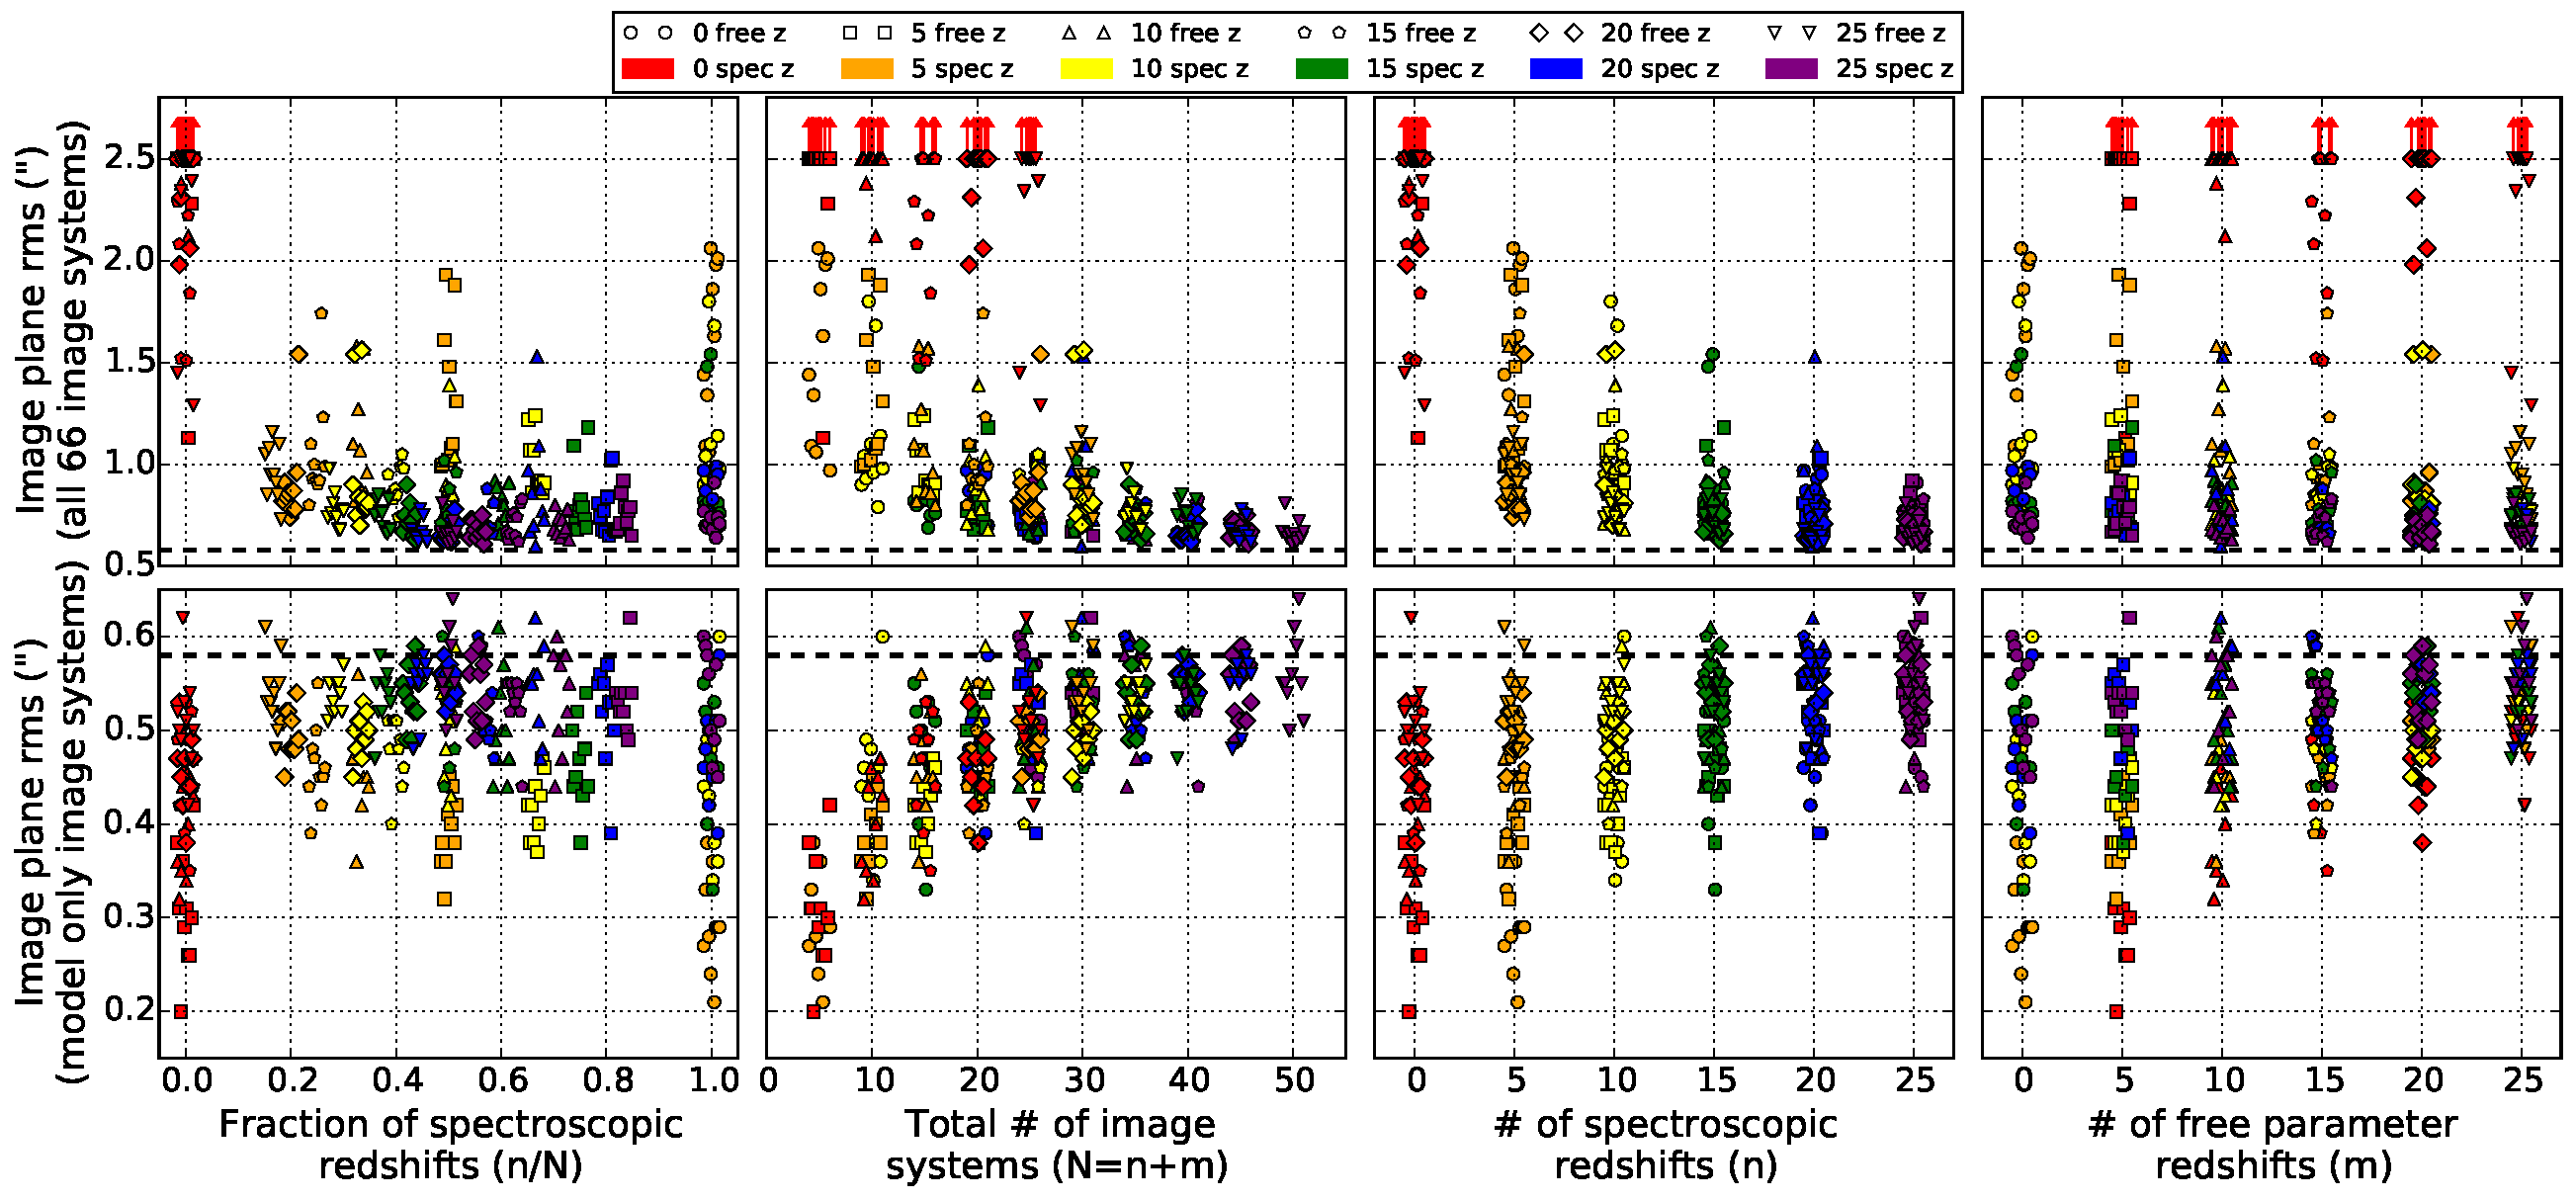
\includegraphics[width=\textwidth]{Chap3/c3f3.pdf}
\caption[Image plane rms vs. spec-z fraction of test models]{Image plane rms for all the test models plotted versus fraction of spectroscopic redshifts, total number of image systems, number of spectroscopic redshifts, and number of free parameter redshifts. The colors and shapes of the points represent the number of spectroscopic redshifts and number of free parameter redshifts used in the model, respectively (see legend at top). The top panels show the image plane rms values computed for all 66 image systems using the true redshift values. The bottom panels show the image plane rms values computed only from the images used as constraints in the lens model and model predicted redshifts.  The dashed line indicates the value of the image plane rms for the fiducial model and is computed from all 66 image systems and true redshifts.}
\label{chap3:fig:rms}
\end{figure*}

\begin{figure*}
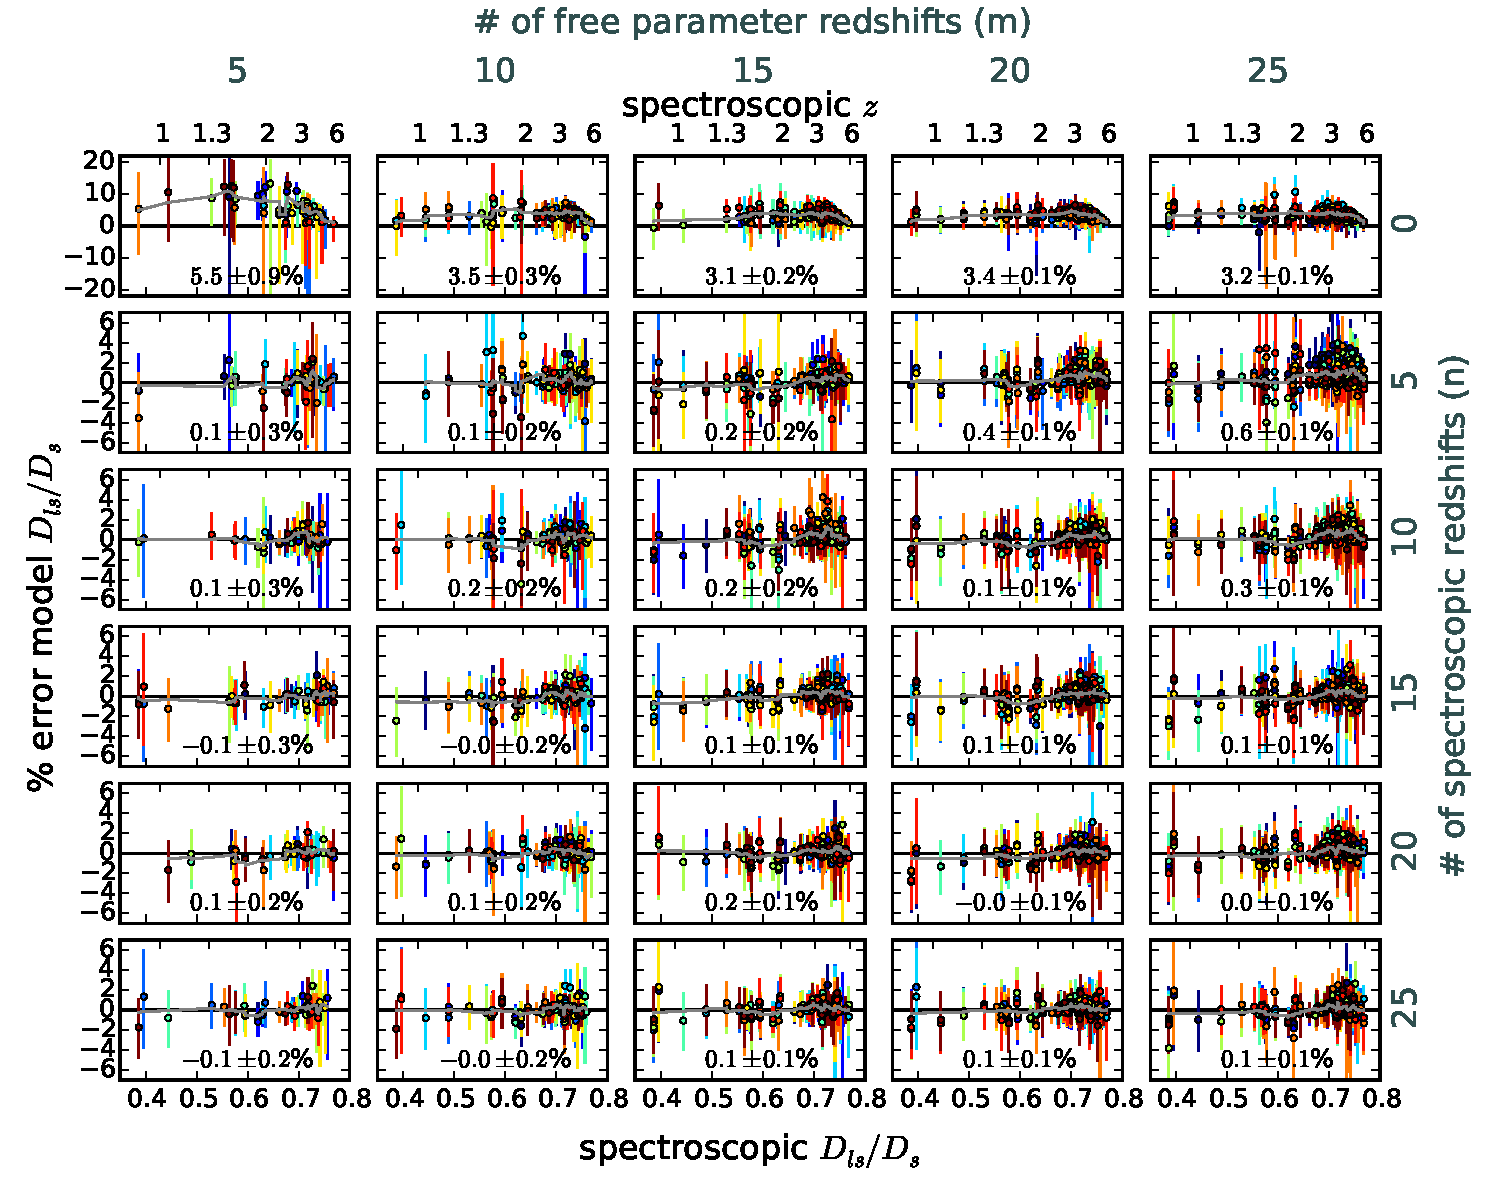
\includegraphics[width=\textwidth]{Chap3/c3f4.pdf}
\caption[Error in redshift parameter of test models]{Error in best fit model redshift parameter of image systems used as constraints in sets of 10 models using different numbers of spectroscopic redshifts and free parameter redshifts. The redshifts are plotted in terms of the lensing fraction $\dls/\ds$, a function of source redshift which scales the deflection angle of the lens. The error bars represent the $1\sigma$ errors computed from the MCMC chain. The colors match the free parameter redshifts used in the same model. The gray line indicates the rolling average across $\dls/\ds$ from all models. The value at the bottom of each is the weighted mean error in the lensing fraction for all models. Note that the top row ordinates have a different scale from the other plots.}
\label{chap3:fig:dlsds}
\end{figure*}

\subsection{Model-predicted redshifts}

We investigate how accurately models using free parameter redshifts predict the true redshift of those image systems. Figure~\ref{chap3:fig:dlsds} shows the error between model-derived redshift and the true redshift of the system. We plot these errors in terms of the lensing fraction $\dls/\ds$ rather than $\zs$; as shown in (\ref{intro:eqn:dlsds}), the deflection angle tensor $\alpha_{ij}$ scales linearly with the lensing fraction. The typical error in model predicted $\dls/\ds$ is $<2\%$ in all cases and tends to be lower for models that have higher fractions of image systems with spectroscopic redshifts. Interestingly, models with low fractions of image systems that have spectroscopic redshifts tend to predict redshifts solutions that are more often biased to higher values for systems with  $z>2$. Nearly all of the model-predicted $\dls/\ds$ of models with $n=0$ are biased high by 5-10\%.

\subsection{Mass}
In Figure~\ref{chap3:fig:mass}, we plot the projected mass profile of the cluster for the fiducial model (top) and residual from the fiducial model for all of the test models (bottom). We find that the errors in the enclosed mass are typically $<4\%$ out to 1 Mpc for models with $n>0$. Models with $n=0$ are generally biased toward lower masses, which is consistent with model predicting higher redshifts for the free parameter image systems. For models with $n>0$, the errors are generally lowest at radii around the ``arc radius", $r_\mathrm{arcs}=305$ kpc, defined as the median image plane projected distance of images used as constraints in the fiducial model; it is comparable to the formal definition of the Einstein radius. Test model combinations with at least five spectroscopic redshifts have errors $<1\%$ around the arc radius.

\begin{figure*}
\center
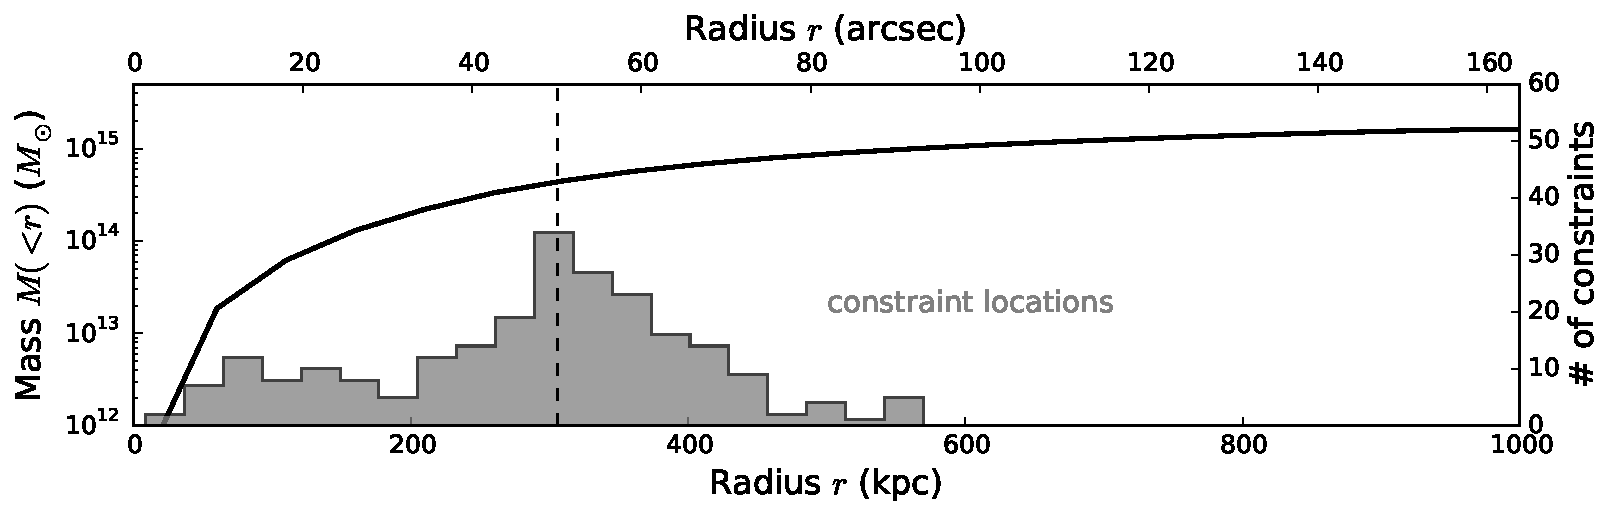
\includegraphics[width=\textwidth]{Chap3/c3f5a.pdf}
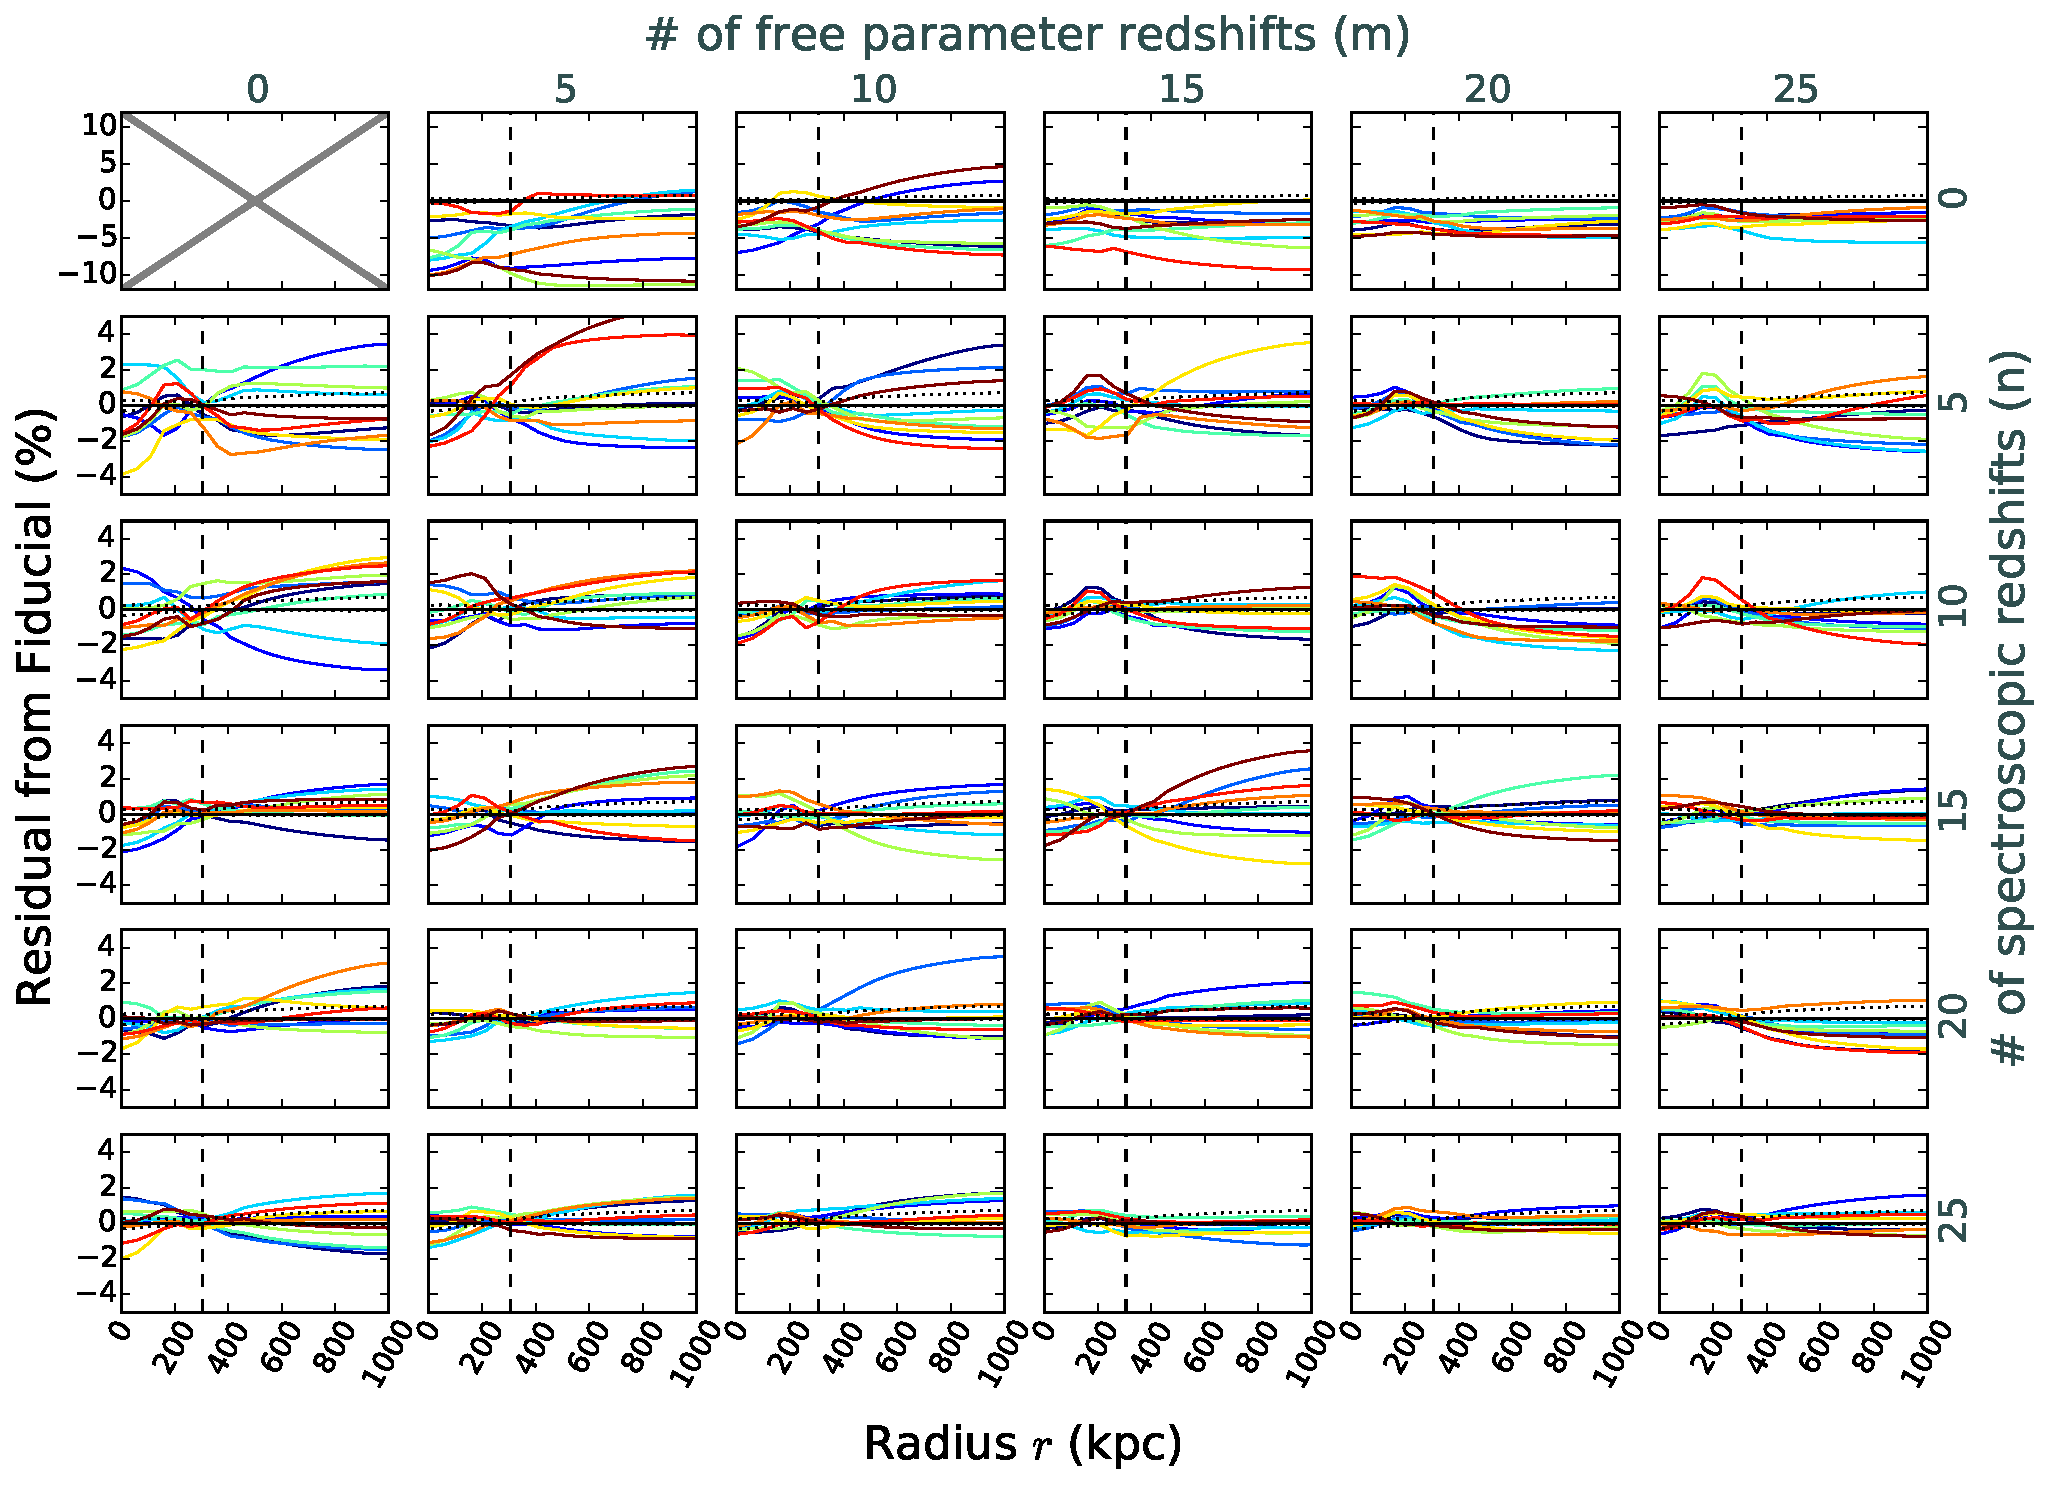
\includegraphics[width=\textwidth]{Chap3/c3f5b.pdf}
\caption[Radial mass profile of Ares fiducial lens model and of test models]{(Top) radial mass profile for the fiducial model. The histogram shows the projected radii of all the constraints used in the model. The dashed vertical line is the median projected radius of the arcs at $r_\mathrm{arcs}=305$ kpc. (Bottom) Radial mass profile residuals from the fiducial model for all test models with different numbers of spectroscopic and free parameter redshifts used as constraints. The dotted lines represent the $1\sigma$ statistical error in the fiducial model mass profile estimated from the MCMC. The dashed vertical line matches $r_\mathrm{arcs}$ from the top plot. Note: the top row ordinates have a different scale from the other plots.}
\label{chap3:fig:mass}
\end{figure*}

\subsection{Magnification}
\label{chap3:subsec:magnification}
%The magnification describes the amplification of the solid angle of a lensed object from source plane to image plane and is derived from the lensing Jacobian tensor
%
%\begin{equation}
%A_{ij}\equiv \frac{\partial\beta_{ij}}{\partial\theta_{ij}}=\delta_{ij}-\frac{\partial\alpha_{i}}{\partial\theta_{j}},
%\end{equation}
%
%\noindent which describes the translation from source plane $\beta$ to image plane $\theta$. The magnification $\mu$ is the inverse determinant of this tensor,
%
%\begin{equation}
%\mu = \frac{1}{|\det A_{ij}|},
%\end{equation}
%
%\noindent which becomes a non-linear combination of first-order derivatives of $\alpha$. Based on its complexity, we expect the magnification factor to have more complicated relations with observable quantities than the diagnostics discussed earlier.

\begin{figure*}
\center
\includegraphics[width=1.0\textwidth]{Chap3/c3f6.pdf}
\caption[Error in magnification of test models]{Median error in the magnification maps for $z=2$ for each set of models with various numbers of constraints with spectroscopic redshifts and free parameter redshifts. The error is computed with respect to the magnification map of the fiducial model. The $z=2$ critical curve for the fiducial model is shown in the solid green and the region enclosed by the dashed green line is the extent of image multiplicity for sources at $z=2$. The top-left panel shows the statistical errors in magnification for each pixel of the fiducial model. Each panel has dimensions $200"\times200"$.}
\label{chap3:fig:magnification_bias}
\end{figure*}

In Figure~\ref{chap3:fig:magnification_bias}, we plot the error in magnification at each image plane position corresponding to a source at $z=2$ for each test model combination (i.e., median magnification of each pixel across all models with same $n,m$) relative to the fiducial model magnification. These maps effectively show the bias in magnification when selecting $n,m$. We choose to display $z=2$ because it corresponds to a middle value of $\dls/\ds$ for all the sources used as constraints.

For models with $n>0$, the magnification errors are all quite similar. Across all models the magnification is most accurate in regions of lower magnification ($\mu<10$) and along the straight portion of the critical curve, the region where most of the multiple images are located. A straight critical curve implies that the vector of the deflection angle is nearly constant in terms of direction and only changes in amplitude; solving the lens equation in this region becomes one dimensional. At the high-curvature portions of the critical curve, the tangential shear is strong and the deflection angle changes rapidly in both amplitude and direction. Also, objects here are highly magnified, but their image multiplicity becomes unity. These singly-imaged sources are indeed strongly lensed, but are not used as strong lensing constraints for this modeling method. Some methods can use single images as constraints; however, doing so greatly increases computing time in order to reject models producing multiple images. Additionally, the flexion of these highly magnified single-image systems could be included in modeling methods to better constrain the mass distribution where there are no multiple images \citep[ex.,][]{Cain:2011ab}.

\begin{figure*}
\center
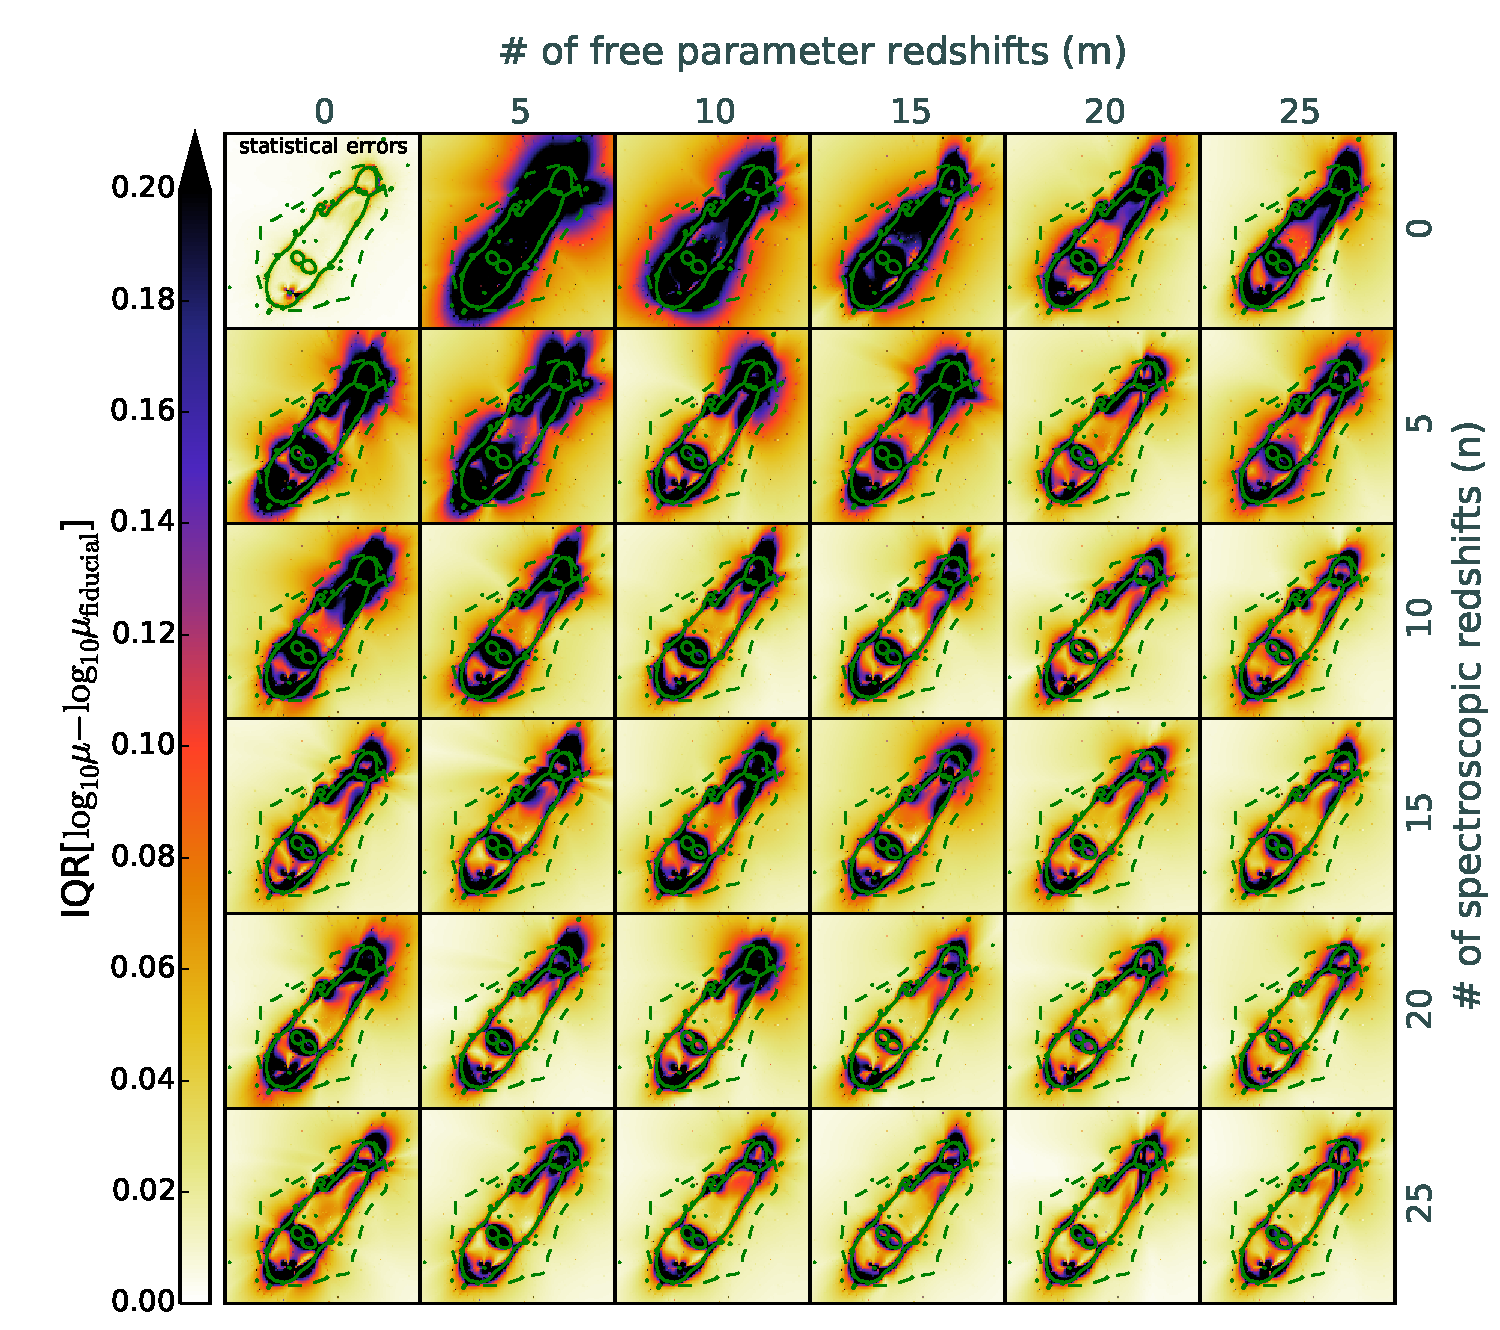
\includegraphics[width=1.0\textwidth]{Chap3/c3f7.pdf}
\caption[Range of error in magnifications of test models]{Interquartile range (IQR) of errors in the magnification maps for $z=2$ for each set of models with various numbers of constraints with spectroscopic redshifts and free parameter redshifts. The error is computed with respect to the magnification map of the fiducial model. The $z=2$ critical curve for the fiducial model is shown in the solid green and the region enclosed by the dashed green line is the extent of image multiplicity for sources at $z=2$. The top-left panel shows the statistical error range in magnification for each pixel of the fiducial model. Each panel has dimensions $200"\times200"$.}
\label{chap3:fig:magnification_spread}
\end{figure*}

While Figure~\ref{chap3:fig:magnification_bias} shows the bias of the magnification for all regions in the image plane over a slew of different models, Figure~\ref{chap3:fig:magnification_spread} shows the interquartile range (IQR\footnote{We define the IQR as the difference between the 75th and 25th percentile models. These percentiles correspond to the average magnification between the 8th/9th-ranked and 2nd/3rd-ranked models, respectively.}) in magnification, i.e., how consistent the systematic errors in magnification are relative to the fiducial models when different sets of constraints are used for the same $n,m$. We plot the IQR to eliminate the effects of potential outlying models in our analysis. We see similar trends to those of Figure~\ref{chap3:fig:magnification_bias}: the IQR in magnification between models is lower for regions with low magnification and along the straight portion of the critical curve. We see a very clear trend with reduced spread in magnification error throughout most of the image plane with higher $N$.

\begin{figure*}
\center
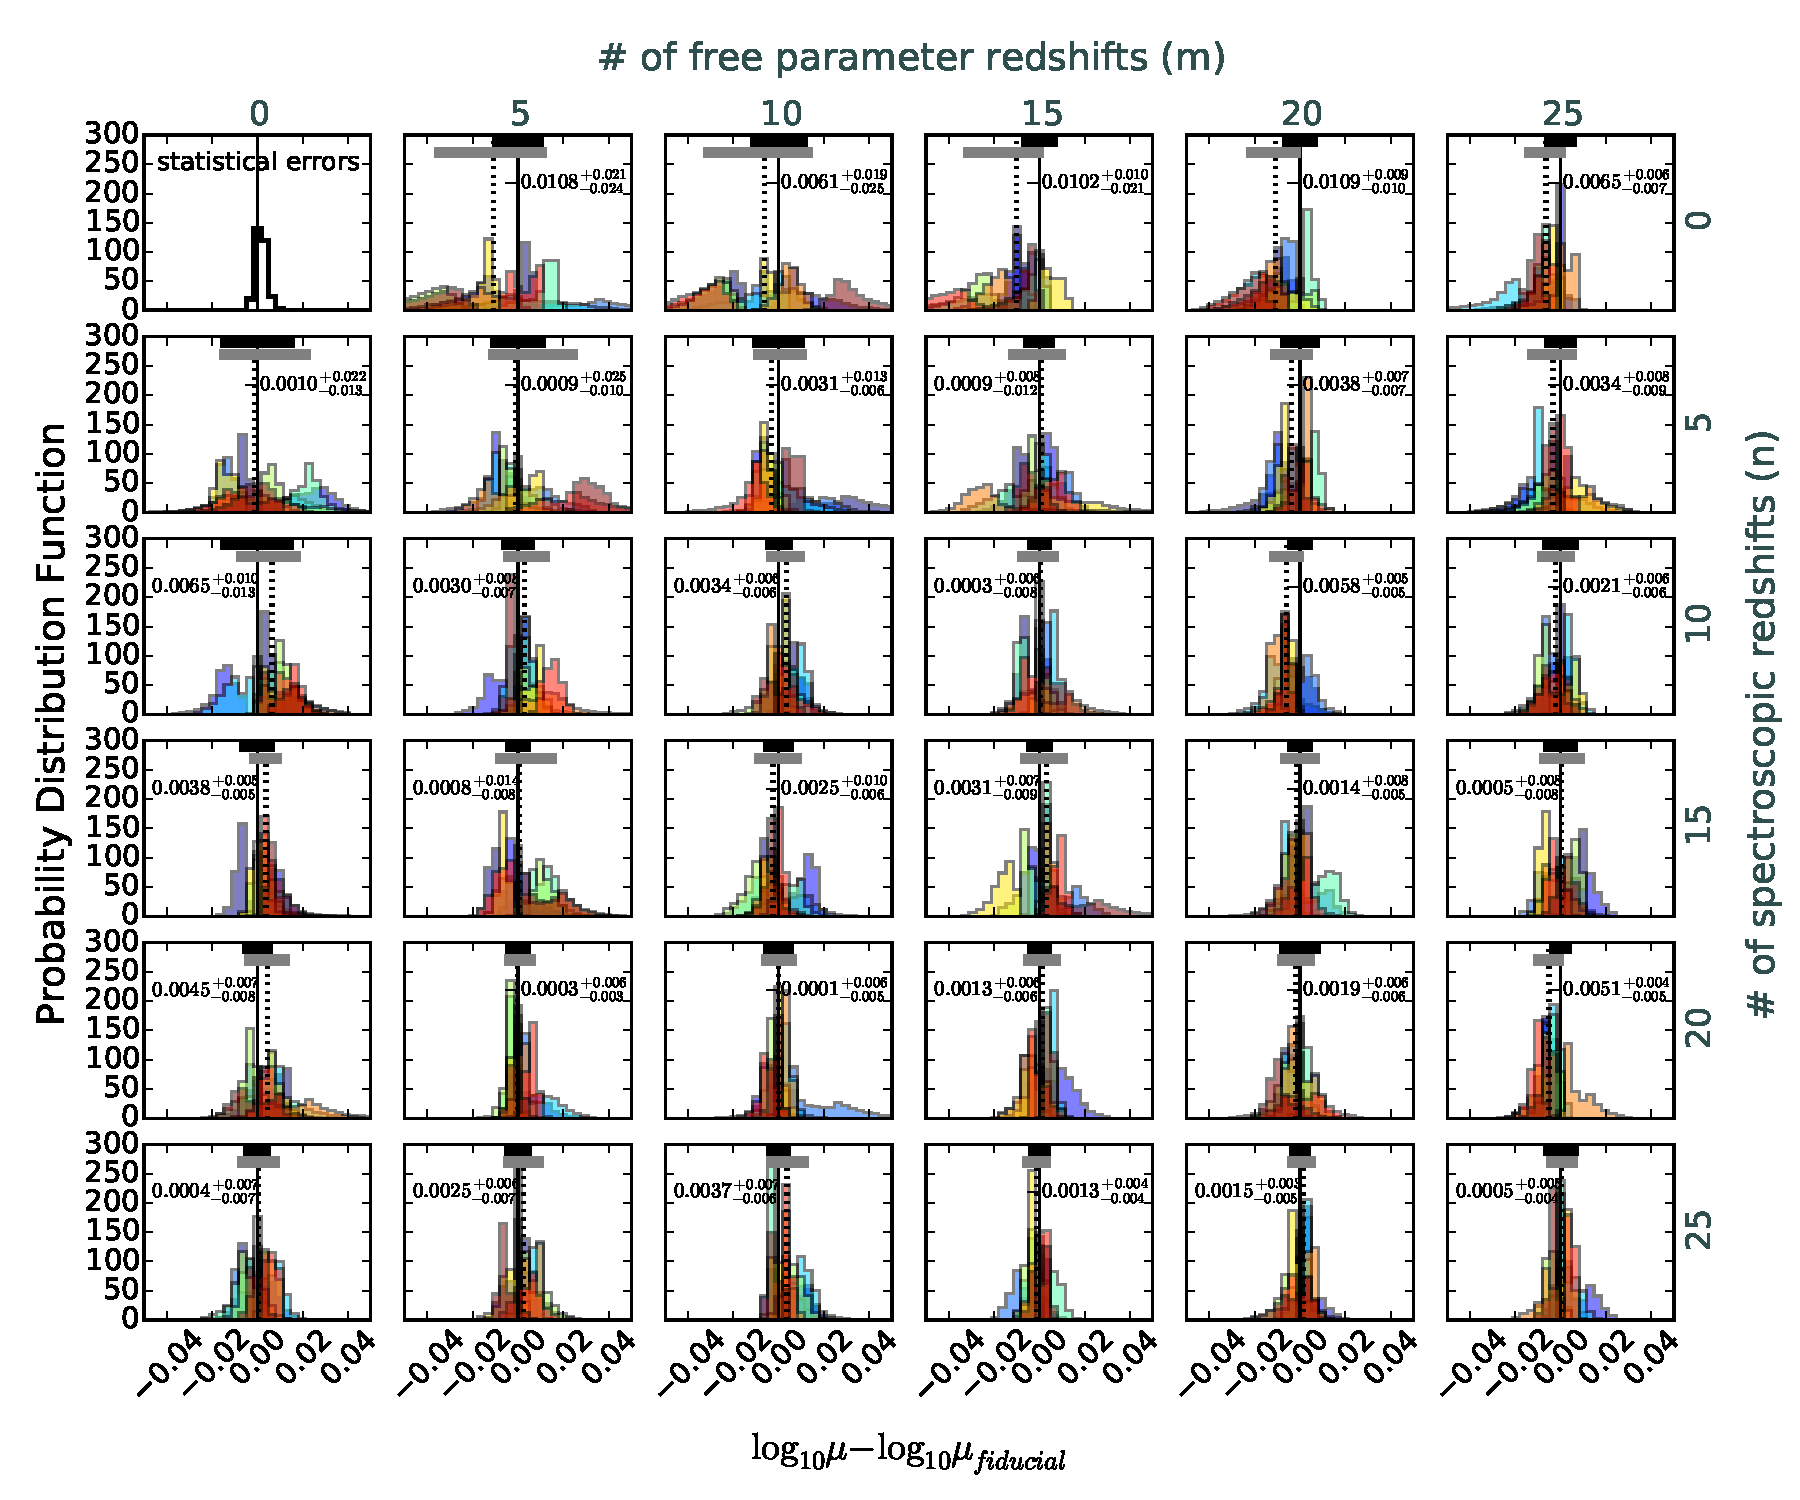
\includegraphics[width=1.0\textwidth]{Chap3/c3f8.pdf}
\caption[Histogram of pixelized-magnification errors of test models]{Histograms of magnification error ($z=2$) for the region of pixels shown in Figure~\ref{chap3:fig:hst} for models with different numbers of spectroscopic and free parameter redshifts. Each color shade represents a unique model constructed with different random subsets of images used as constraints. The top-left panel shows the $1\sigma$ statistical errors of each pixel in the fiducial model. The black bar on top shows the typical $1\sigma$ statistical error for a test model. The dashed vertical line and horizontal grey bars show the median and $1\sigma$ range in magnification error distribution of all test models combined, and these values are displayed in each panel.}
\label{chap3:fig:histograms}
\end{figure*}

We attempt to quantify the systematic errors in Figure~\ref{chap3:fig:histograms} by looking at the distribution of magnification errors across the image plane. We create histograms of the magnification error for each pixel for each individual test model. We only examine pixels located in a rectangular region with bounds selected arbitrarily such that it lies in the lower right $(+x,-y)$ aligned roughly with the critical curve of the cluster, to avoid pixels near the curved portion of the critical curve. This region of pixels is shown in Figure~\ref{chap3:fig:hst}. We also only select pixels with $\mu_\mathrm{fiducial}<20$ to avoid high magnifications induced locally by cluster member galaxies. We see that models with lower $N$ tend to produce magnifications that are typically biased low, however, beyond $N\geq25$ the distributions of models appear to be similar and with negligible bias, with a typical error of about 2\%.

It is noticeable across all test models that the variation in the distribution of magnifications is quite significant for low total number of image systems, even amongst test models with identical $n,m$. This indicates that it is not necessarily quantity of image systems or redshifts, but rather the selection of these constraints that drives systematic error. We examined closely a few of the models with outlying distributions in Figure~\ref{chap3:fig:histograms} and found that the random selection of spectroscopic redshift systems for those models was either unevenly distributed spatially in the image plane or unevenly distributed in redshift space.

\begin{figure*}
\center
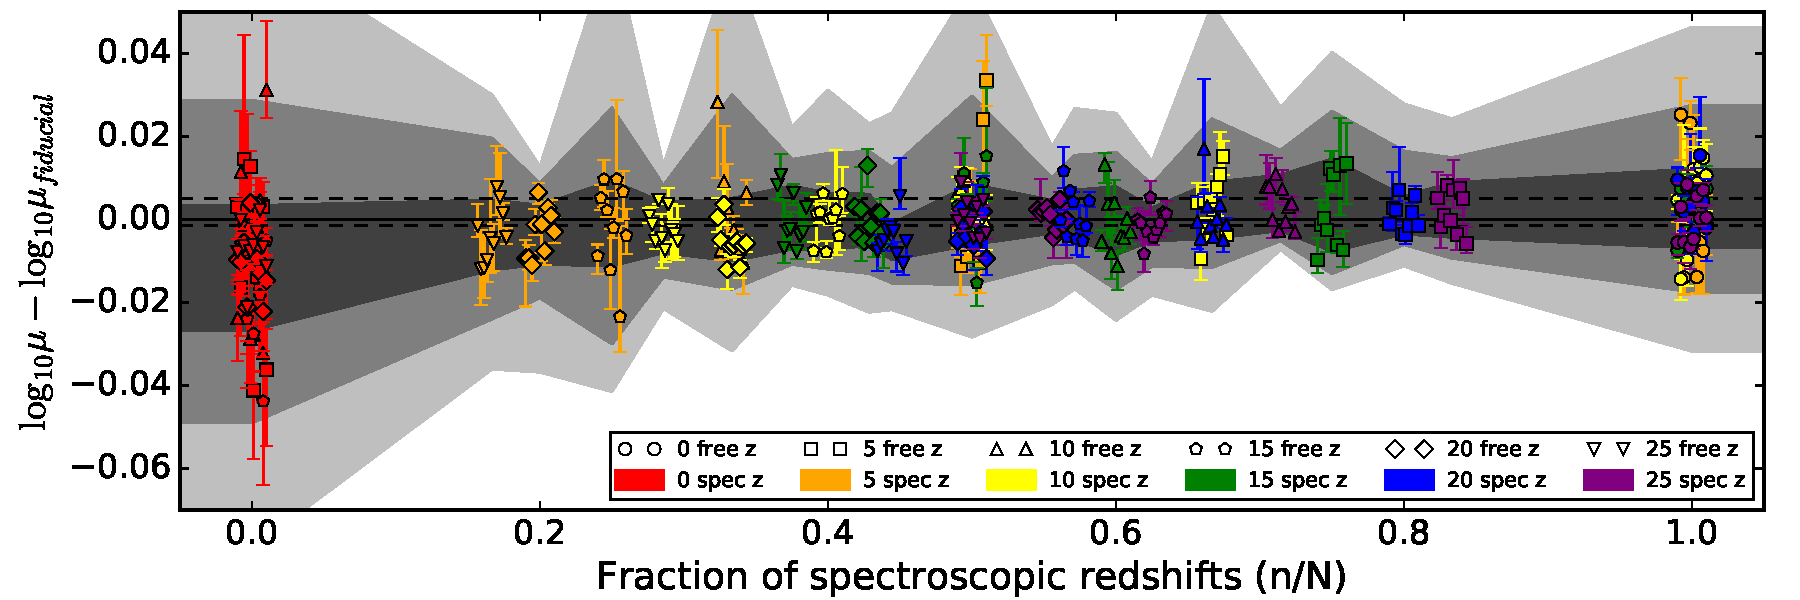
\includegraphics[width=\textwidth]{Chap3/c3f9a.pdf}
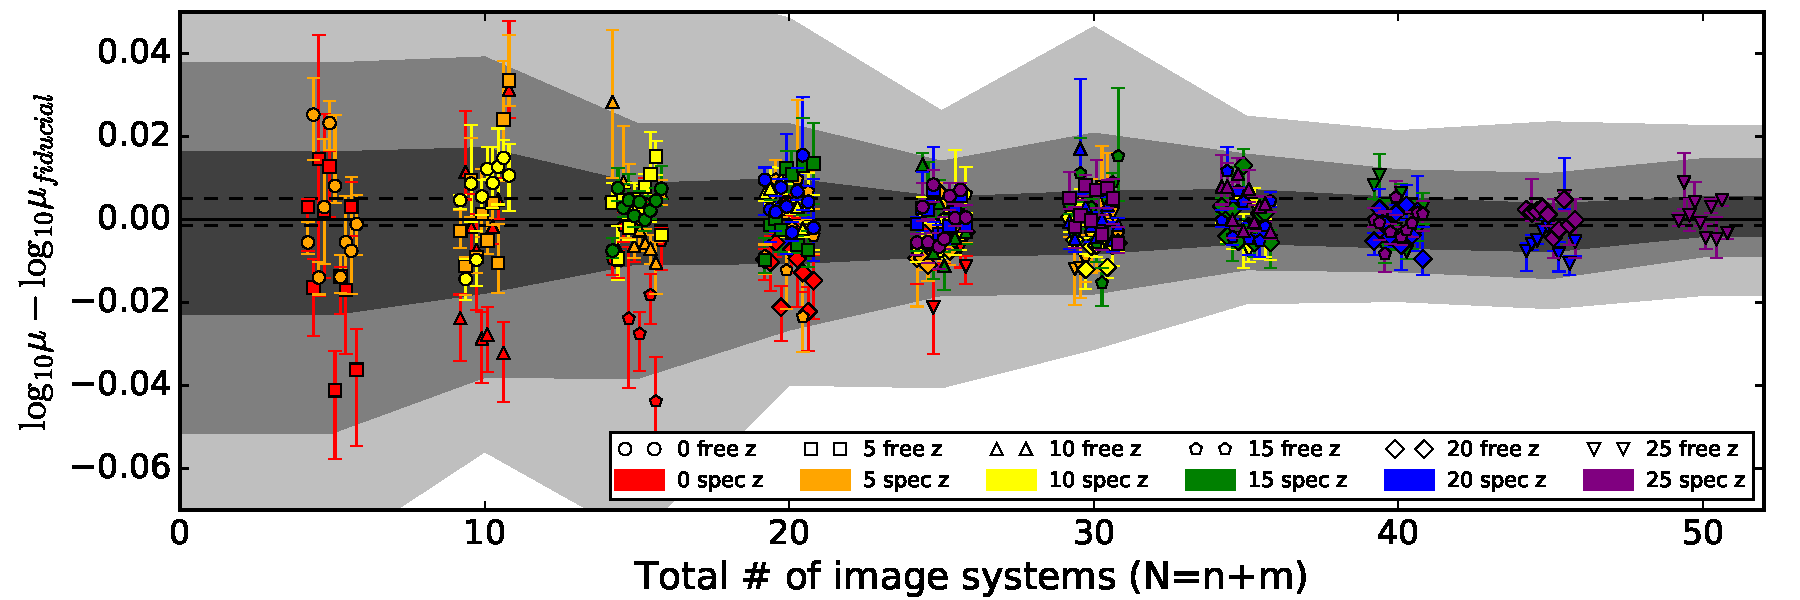
\includegraphics[width=\textwidth]{Chap3/c3f9b.pdf}
\caption[Magnification error vs fraction of spec-z and vs total number of images for test models]{The relative magnification error ($z=2$) for the region of pixels shown in Figure~\ref{chap3:fig:hst} for all the test models versus fraction of spectroscopic redshifts $n/N$ (top) and total number of image systems $N$ (bottom). The values are median and $1\sigma$ range of values within the region for the best fit models. The different shapes and colors indicate the number of free parameter redshifts and spectroscopic redshifts used in the model, respectively. The dashed lines indicated the $1\sigma$ statistical errors for the fiducial model. The gray contours represent the 1, 2, and 3$\sigma$ ranges for each block of the test models in fraction/number of systems. Note: the abscissa values for the test models within each grouping of test models have been slightly offset horizontally for display purposes. There is a clear trend of improved magnification error with the total number of images, but no dependence on the fraction of spectroscopic redshifts.}
\label{chap3:fig:specz_fraction}
\end{figure*}

In Figure~\ref{chap3:fig:specz_fraction}, we plot the relative magnification error and spread for all test models (defined as they are in Figure~\ref{chap3:fig:histograms}) versus the fraction of spectroscopic redshifts $n/N$ and total number of image systems $N$. We report no clear trend in magnification error or spread with spectroscopic redshift fraction, except that models with no spectroscopic redshift are biased toward lower magnifications and have a $1\sigma$ spread of about 3\%.  There is a clear trend in decreasing systematic error with $N$, and for $N\geq25$, the $1\sigma$ magnification error stays constant at about 1\%.

%==================================================================================
%   DISCUSSION
%==================================================================================
\section{Discussion}
\label{chap3:sec:discussion}

\subsection{Number of image systems in a model}
The selection of image systems with or without confirmed redshifts is usually not a choice in building a lens model, as for most clusters the number of constraints is small regardless and thus modelers require a minimum number of constraints to build a statistically meaningful model. However, the paradigm has changed with the onset of the HFF, where there is a seemingly-infinite number of multiple image systems and several spectroscopic redshifts from which to build our models. Statistical errors in these scenarios are now much lower than the systematics, so including or rejecting a candidate image systems in a model is now a question of its influence on systematic error.  Our results show that models reach a threshold in systematic errors across all diagnostics once $N\geq25$ and $n>0$ have been established. For the test models, the identification of images and redshift measurements are known with certainty; however, that is not the case in real scenarios. Beyond this threshold, rejecting an incorrect image system or redshift based on a high degree of uncertainty will likely deflate rather than inflate systematic errors.

\subsection{Finding new multiple image systems}
From Figure~\ref{chap3:fig:rms} we learned that spectroscopic redshift systems are needed to improve the image plane rms of a model when few constraints are available ($N<15$). While this may have its applications post-modeling, image predictability is most applicable for improving an existing model by using its deflection to find new multiple image systems. The results of this work emphasize the importance of including more spectroscopic redshifts early on in the stages of lens modeling, as models built using fewer spectroscopic redshifts have more error in predictability and thus are more likely to find false image systems. While the brightest and largest multiple image systems are obvious by morphology and color without confirmed redshifts, fainter and smaller systems are more ambiguous, especially where many faint galaxies at all redshifts pass the detection limit and could be confused for lensed galaxy candidates.

\subsection{Constraining mass}
Mass profiles of galaxy clusters are quite robust to redshift confirmation of multiple image systems. Figure~\ref{chap3:fig:mass} shows that including more image systems in a model with at least a handful of spectroscopic redshifts helps to reduce systematic errors in mass profile. The systematic error on total projected mass out to 1 Mpc is only 2\% for models with $N\geq25$ and $n>0$ (4\% for $N<25$). This result is promising for using strong lensing clusters for cosmology -- future large area surveys will find hundreds of clusters and complete spectroscopic follow-up will not be a feasible task. Knowing that mass within the Einstein radius has low systematic errors will add further significance to cosmological models constrained by strong lensing masses. However, these low errors lie on top of statistical errors and systematics due to structure along the line of sight. We note that we only investigated the mass profile of a single, massive cluster in this work. It would be important in future work to test if this result holds for less massive clusters that lens only a handful of images.

\subsection{Improving magnification estimates}
We find that the regions of the lens map with the highest systematic error are those close to the critical curve and/or along portions with significant curvature where the shear is high and there are few multiple images. The lowest error regions are those covered by multiple images, along portions of the critical curve that are straight. We found that models with low $N$ and low $n$ tend to estimate lower magnifications overall. As we saw, the free parameter redshifts solved for in models with many free parameter redshifts tend to be biased high, which results in a lower mass and thus lower magnification, which matches the trends we see in Figures Figure~\ref{chap3:fig:dlsds}-Figure~\ref{chap3:fig:histograms}. While mostly qualitative, this information is useful for anyone questioning the accuracy of a magnification value. While it is trivial to estimate the magnification and statistical uncertainties for a single image plane position by blindly computing it for one pixel in a magnification map, one needs to consider the pixel position within the full image plane to begin estimating the systematics.

\subsection{Models without spectroscopic redshifts}
Since the deflection angle depends on source redshift, the mass estimate within the Einstein radius depends on the redshift of the multiple images. If the redshift of the source is unknown, then the mass is degenerate with redshift. Therefore, lens models need at least one spectroscopic redshift to break the degeneracy. We test this theory by running models without spectroscopic redshifts and find that it is indeed the case that models built with even a handful of spectroscopic redshifts outperform all models built without any spectroscopic redshifts across all of our diagnostics. The models tend to predict redshifts that are higher than truth for nearly every image system, and therefore under-predict the mass by up to 10\% at the Einstein radius, and produce magnifications that can be either highly under- or over-predicted depending on the selection of constraints. When also factoring in statistical errors, which are high for low $N$ systems, and other systematics like structure along the line-of-sight, any lensing outputs from models with no spectroscopic redshifts should be treated with caution.

\begin{figure*}
\center
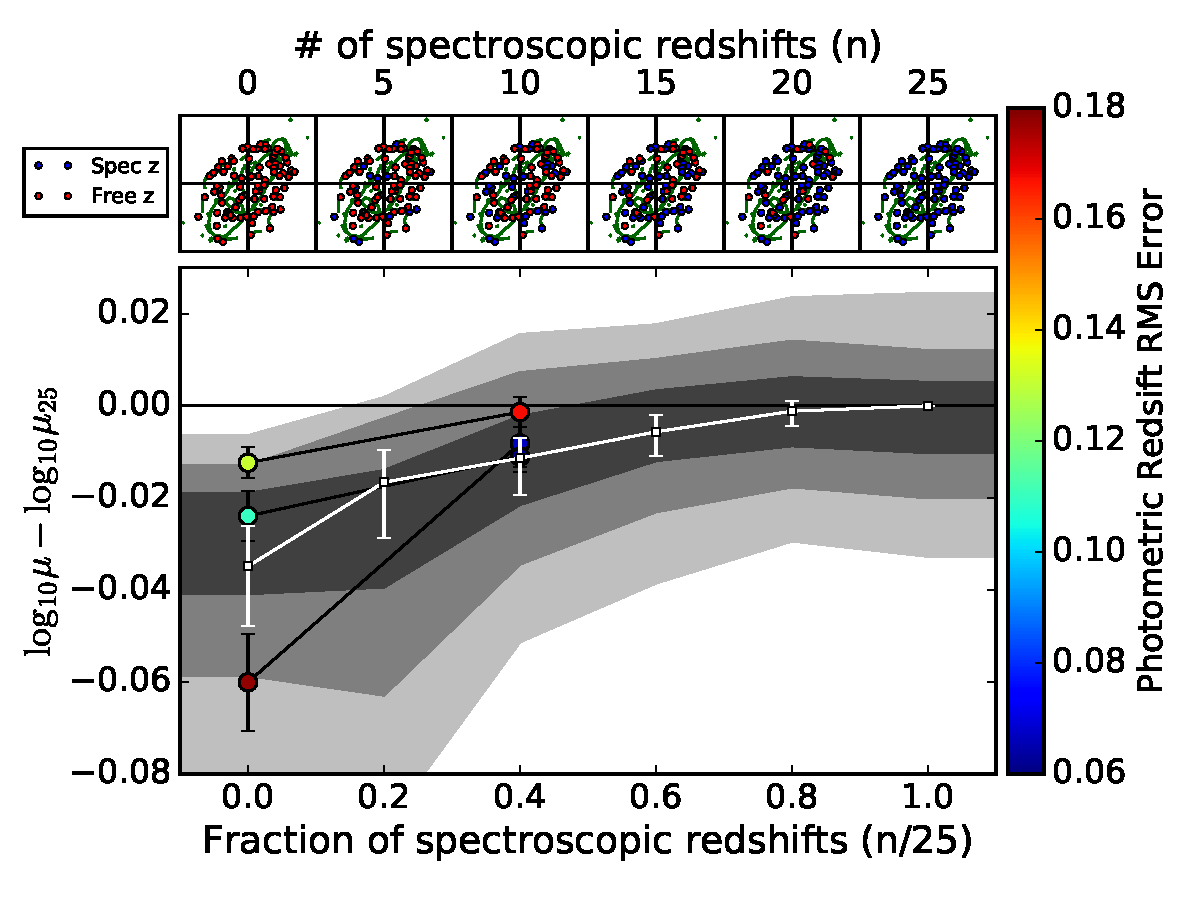
\includegraphics[width=0.8\textwidth]{Chap3/c3f10.pdf}
\caption[Relative magnification error of single model with increasing spec-z fraction]{The relative magnification error in ($z=2$) for the region of pixels shown in Figure~\ref{chap3:fig:hst} versus fraction of spectroscopic redshift systems for six lens models built using the same 25 image systems. The first model uses no spectroscopic redshifts, the second model adds spectroscopic redshifts to 5 systems, the third model adds spectroscopic redshifts to 5 more systems (10 total), etc. until all systems have spectroscopic redshifts. The errors are with respect to the model with all 25 spectroscopic redshift systems. The values are the median and $1\sigma$ range of values with the region of the best fit model. The gray contours represent the 1,2, and 3$\sigma$ statistical errors estimated from the MCMCs. The top row shows the image plane positions of the images from the 25 systems used as constraints. The blue and red points represent systems with and without spectroscopic redshifts, respectively. Each map is $200"\times200"$ centered on the origin defined in Figure~\ref{chap3:fig:hst}. The green solid and dashed lines indicate the locations of the $z=2$ critical curve and region of multiple images, respectively. The colored circles represent models using the same constraints as the models shown in the maps above; however, photometric redshift measurements are used as the priors for the free parameter redshifts rather than a uniform random prior. The colors indicate the rms error in the photometric redshifts used for that particular model: $(z_\mathrm{spec}-z_\mathrm{phot})/(1+z_\mathrm{spec})$ (see \S~\ref{chap3:subsec:photoz}).}
\label{chap3:fig:single_compare}
\end{figure*}

\subsection{Increasing the number of spectroscopic redshifts in a single model}
\label{chap3:subsec:n_specz}
Our results in \S\ref{chap3:subsec:magnification} showed that there was no trend in systematic errors on magnification with the fraction of spectroscopic redshifts used in a model when considering random selections of $n,m$. However, in cluster lensing scenarios similar to the HFF, the selection of image systems mostly stays the same and the fraction of spectroscopic redshifts $n/N$ increases over time as more spectroscopic data are collected. On-going lensing analyses of the HFF have so far indicated that increasing the fraction of spectroscopic redshifts for a given cluster may decrease systematic errors on its lens models. The tensions between observations of Supernova Tomas in Abell 2744 and Supernova Refsdal in MACS J1149.6+2223 and the predictions from several different lens models (i.e., magnification, time delays) have weak negative correlations with fraction of spectroscopic redshifts \citep{Rodney:2015uq,Rodney:2016sf}. In this scenario, the lens models are built by different teams using nearly the exact same identifications of multiple image systems, with some models including new spectroscopic systems in addition to existing sets.

To test whether we see this trend in the simulations, we design a set of lens models that represent a progression in increasing spectroscopic redshift fraction. We construct six new lens models of Ares each using the same set of 25 image systems. The first model is constructed without any spectroscopic redshifts, the second adds spectroscopic redshifts to 5 of these systems, the third adds an additional 5 spectroscopic redshifts to the existing 5 (10 total), etc., until all image systems have spectroscopic redshifts. The 25 systems and each addition of spectroscopic systems are selected carefully in order to maintain a roughly uniform distribution of locations in the image plane and of redshift. Figure~\ref{chap3:fig:single_compare} shows the magnification error of these models with respect to the model with $n=N$, in the same manner as Figure~\ref{chap3:fig:specz_fraction}. Here, it is clear that the accuracy of the magnification estimates improves with increasing $n/N$, indicating that measuring the spectroscopic redshifts of known lensed galaxies that are used as constraints will help decrease systematic errors while the precision is set based on the total number of systems. This result is consistent with those of \citet{Rodney:2015uq,Rodney:2016sf}, but shows a much stronger correlation. It is likely that the trends in the HFF models are weakened by systematics in the modeling methods themselves and that the selection of constraints were not exactly identical between models.

It is still important to note, however, that the model with $n=N$ is offset in magnification error from the fiducial model by about -0.01 mag. This result is expected, as we saw in Figure~\ref{chap3:fig:histograms} that models with $n=25,m=0$ have a systematic error of 0.02 mag with respect to the fiducial. With this in mind, increasing $n/N$ for a single model is most effective at decreasing systematic errors in magnification up to about $n/N\sim0.5$. Beyond that, the exact selection of all the image systems used in the model is a more significant source of systematic error.

While an investigation of the effect of photometric redshift information is beyond the scope of this paper, we do include a test case where we constrain the free redshift parameters with priors from photometric redshift catalogs. This preliminary analysis indicates that photometric redshifts may increase the accuracy of the lens model, but can also result in significantly inaccurate results if not handled with care. We discuss this in \S~\ref{chap3:subsec:photoz} below.

\section{Future work}
\label{chap3:sec:future}
While we have begun to thoroughly investigate the systematics of lens modeling in this paper, there are still many contributing factors we have not yet explored. Here, we considered how using different random subsets of spectroscopic and free parameter redshift image systems in a strong lens model affects the resulting multiple image predictability, mass profiles, and magnifications. As stated above, these results suggest that the exact selection of constraints and redshift information may be more influential on systematic errors then quantity, especially for the values of the magnification. Thus, we plan to follow up investigations of constraint selection in our continuation of this work.

\subsection{Observational limits on constraint selection}
We know the selection of multiple image systems is not random by any means and is a function of image brightness, which depends on the source's intrinsic brightness, luminosity distance from observer, and magnification induced by the galaxy cluster. The faintest observed images are less likely to be identified as multiple images. Similarly, obtaining spectroscopic redshifts can depend on image brightness, redshift, and image plane position. Multi-object spectrographs are limited in slit-packing capabilities and may only target the brightest systems for redshift measurements. Spectra of images close to cluster member galaxies might be contaminated, for which may make determining a redshift more difficult. \hst\ grism spectroscopy and integral field spectrographs are able to target many more images; however, they tend to have a limited total field-of-view. Additionally, completeness of spectroscopic redshifts depends on redshift as bright emission lines get shifted out of the instrument's wavelength coverage for certain redshifts, the so-called ``redshift desert" where redshifts become more challenging to measure. Factoring these selection effects could highlight position and redshift dependencies on the systematic error induced by spectroscopic selection effects.

\subsection{Photometric redshifts}
\label{chap3:subsec:photoz}
The current analysis clearly leaves out possible useful information in the form of photometric redshifts; these are typically available for clusters with extensive multiwavelength imaging data. Photometric redshift measurements are prone to their own systematic errors, and while these measurements can become more precise with increased number of bandpasses and deeper data, catastrophic failures can still occur. Photometric redshift measurements can be implemented in the lens modeling process by using the posterior probability distribution for the photometric redshift as the prior for the free parameter redshift in the lens modeling. While we leave a thorough investigation of the affect of photometric redshifts on lensing systematics for future work, we present here a case study.

We re-run the models we used in \S~\ref{chap3:subsec:n_specz} with $n=0$ and $n=10$ three more times using different realistic photometric redshift estimates for the priors of images without spectroscopic redshifts. In this experiment, the lensed galaxies used as constraints with spectroscopic redshifts are treated the same as before. However, lensed galaxies without spectroscopic redshifts are not assigned a uniform random prior on their free parameter redshift, but rather a gaussian prior centered on an assumed photometric redshift. We use the ASTRODEEP photometric redshift catalogs for HFF clusters Abell 2744 and MACS J0416 \citep{Castellano:2016lr} to determine our realistic photometric redshift measurements, and supplement the spectroscopic redshift sample of MACS 0416 with the MUSE redshifts measured by \citet{Caminha:2017rw}. We use the spectroscopic and photometric catalogs from this sample to estimate the accuracy of a photometric redshift given its true redshift. For each galaxy in our models of Ares where we do not include the spectroscopic redshift as a constraint, we draw a galaxy from the ASTRODEEP catalog with a similar spectroscopic redshift to its true redshift in the Ares simulation (within $0.04(1+z_\mathrm{true})$). We then assign the photometric redshift estimate obtained for that ASTRODEEP galaxy as the center of gaussian prior for the Ares galaxy. We assign a typical statistical error on photometric redshifts from the ASTRODEEP catalog as the width of the gaussian prior (these errors can vary significantly from galaxy to galaxy and across redshifts, from a few percent to up to 50\%.) This procedure results in a realistic representation of scatter of photometric redshift values at a fixed spectroscopic redshift, as well as the rate of catastrophic failures in fields that are by construction similar to our simulation. We include these models in Figure~\ref{chap3:fig:single_compare} as colored circles, where the color matches the rms error in photometric redshift. The results show that photometric redshifts can improve the lens modeling process, however, only when the photometric redshifts are relatively accurate. As shown in Figure~\ref{chap3:fig:single_compare}, using only photometric redshift priors can actually increase systematic errors in magnification over the use of broad uniform random priors when there are catastrophic failures in the photometric redshift measurements. One of the models we used had no spectroscopic redshifts and a photometric redshift rms error of 0.18, including a catastrophic failure with $z_\mathrm{phot} = 1.06$ for $z_\mathrm{spec} = 5.34$. This model produced a worse systematic offset in magnifications compared to the fiducial model. After adding 10 spectroscopic redshifts, the rms error dropped to 0.06, likely the result of replacing a catastrophic failure photometric redshift measurement with the true redshift of that system. The resulting model performs slightly better than the model without any photometric redshift information. The two other models with no spectroscopic redshifts had a moderate rms error (0.12) and reduced the systematic error by 0.01-0.02 dex, but did not perform significantly better after adding more spectroscopic redshifts. Photometric redshifts have the highest impact on modeling when there are few to no spectroscopic redshifts; however, this only improves the model if those photometric redshifts are reasonably accurate.

It is worth noting that there are a few aspects of including photometric redshifts in lens modeling that are difficult to simulate because they are highly dependent on the experience of the lens modeler. In the case of the catastrophic failure like in one of the models we tested, it is quite likely a lens modeler would have rejected any low-redshift solutions that are inconsistent with the lensing geometry based on a model produced by the other images with reasonable photometric redshifts (the $z=5$ critical curve has a much larger extent than the $z=1$ critical curve so the multiple images should be closer together). We also are not considering that the individual images may have different photometric redshift estimates. Brighter images may have more robust redshifts while fainter or contaminated images may produce wildly different photometric redshifts. A system of images with significantly different photometric redshifts may be less likely to be identified as a system and therefore not used in the lens model. It is unclear at this point how much more photometric redshifts will improve lens modeling if they are not reasonably accurate. However, future purely photometric surveys will have few if no spectroscopic redshifts for the many thousands of lensing clusters predicted to be found. Thus, it is important to investigate how photometric redshifts impact lens modeling and we plan to do so more extensively in future work.

\subsection{Image multiplicity and misidentified multiple images}
Our analysis in this paper investigated how the number of multiple image systems affects the systematic errors in lens modeling. However, we assume that every image system is equal in constraining power and that each system has been correctly identified. In reality, image systems with higher multiplicity (e.g., 4-image systems versus 2-image systems) have a higher weight in the lens modeling. Additionally, higher multiplicity image systems are likely to include radial arcs that will have higher constraining power on the inner slope of the mass profile. From the suite of 350 models we ran, the average image multiplicity (i.e., average number of images per system) ranged from 2.8 to 3.8 for all combinations of $n,m$. We found no trend in systematic errors in the inner and outer slopes of the mass profile nor the magnifications with average image multiplicity. It is possible trends could occur when the number of image systems is fewer than five, which was the lowest number of systems we investigated. Thus, image multiplicity should be investigated in future work with clusters that have very few multiple image systems to constrain lens models.

We did not account for image identification error in our analysis. The faintest images of a single system are the most likely to be misidentifed as they can easily confused with other background sources or blended with foreground objects. As stated in \S~\ref{chap3:subsec:fiducial_model}, we did not include some of these images that are likely to be misidentified in our models. Therefore, our results show the best case scenario when lens modelers use only the highest-confidence images in their lens models. Simulating the effects of misidentification could be done in future work by comparing models where the faintest image system is perturbed by a several arcseconds or not included in the model.

\subsection{Image plane and redshift distribution of lensing constraints}
For models with smaller numbers of image systems, it is important to assess how the spatial distribution of image systems in the image plane affects systematic errors. We found in this work that many of the outlier test models in mass and magnification had uneven spatial distribution of spectroscopic systems. We also saw that models with smaller $N$ had larger spread in mass and magnification, as the spatial distribution of the constraints can vary significantly from model to model. As more constraints are added, constraints will more evenly populate the multiple image region. Ares simulates a very massive cluster and it is likely that a cluster of this size will lens more than a handful of image systems. Therefore, we did not attempt to model Ares using fewer than five image systems. We would consider instead modeling a less massive cluster to assess how image plane distribution affects the outcome of a lens model.

As we found in this analysis, the elongated mass distribution of Ares across the sky creates an elliptical critical curve, where the magnification errors are lowest along the straight portions of the critical curve. These elongated mass distributions are common amongst the HFF clusters, which lie at the cusp of mass assembly in the nodes of the cosmic web. It would be interesting to investigate systematics on clusters with more spherical mass distributions. A prime example would be Abell 1689, which has a large number of identified image systems with spectroscopic redshifts and for which existing lens models suggest it has a more circular critical curve \citep{Diego:2015tg,Coe:2010fy,Limousin:2007fk,Broadhurst:2005qy}.

The redshift distribution of lensed sources could potentially increase systematic error as well. The sources used in Ares were well distributed across redshifts from $z\sim0.9-6$; however, this is not the case in reality as the luminosity function of galaxies and the area of the caustic region both depend on redshift. There is an observational bias toward selecting the brightest sources, and as lensing conserves surface brightness, this leads to a higher likelihood of low redshift sources being identified and used as constraints in a model. We found that some models that were outliers in our analysis for a given $n,m$ had uneven distributions in redshifts. It is well known that multiple redshifts of sources are needed to establish the slope of the mass distribution in a lens model \citep[i.e., break the mass-sheet degeneracy, see][]{Schneider:1995vn}. In cases where all the lensed sources are low redshift, it is possible to extrapolate the mass to larger Einstein radii and thus predict the magnification of higher redshift sources; however, the accuracy of doing so is unknown and is worth investigating in the future.

\vspace{6pt}

For clusters such as Ares, built to resemble massive lensing clusters such as the HFF, it is safe to say that there will be a wealth of constraints across the image plane and redshift space. More massive clusters have a larger lensing cross section and thus have access to a much larger volume of background sources from which to lens. The investigations into image plane and redshift distribution of lensing constraints is best left to more average mass clusters, which will likely only lens a handful of sources. As Ares is too massive to investigate the parameter space of $N<5$, these questions call for a different design in cluster lensing simulations and are best left for future studies.

%==================================================================================
%  CONCLUSION
%==================================================================================
\section{Conclusion}

We have investigated the systematic errors of parametric strong lensing modeling induced by selection of constraints using our ``unblinded" model of the simulated cluster Ares \citep{Meneghetti:2016xe}. Here we summarize our findings:

\begin{enumerate}
\item The image plane rms based on the full lensing evidence, i.e., the image predictive power of a lens model, improves mostly effectively with increasing number of spectroscopic redshift image systems. This result indicates the necessity for obtaining spectroscopic redshifts early on in the modeling process, as they are crucial to increasing the accuracy of finding new multiple image systems. We also have shown, however, that the image plane rms values quoted in the literature, which are computed only from image systems used in the model using best fit model redshifts, shows the opposite trend. While lower values of the rms computed this way reveal a better model fit with more free parameters and fewer constraints, it can be misleading as a measure of model accuracy.
\item Lens models with at least a handful of spectroscopic redshifts are able to predict the redshifts of image systems without spectroscopic redshifts within 2\% (in $\dls/\ds$); however, they are generally biased higher for image systems with $z>2$.
\item The mass profiles are accurately measured for all variations of lens model constraints with $n>0$: $<4\%$ error within 1 Mpc and $<2\%$ at the cluster Einstein radius.
\item Qualitatively, the magnification error is lowest in regions of the image plane where the multiple images are located and typically along the straight portions of the critical curve. The magnification error is larger at the curved portions of the critical curve and typically biased toward lower values.
\item The accuracy of magnifications increases with total number of image systems, and for $N>20$ plateaus to 2\%. We observe no trend in magnification accuracy with fraction of spectroscopic redshift when comparing models in which $n,m$ are chosen randomly, as long as this fraction is greater than zero. However, we do find that for a model with a fixed set of multiple images, increasing the fraction of systems with spectroscopic redshifts helps improve the accuracy while maintaining nearly a constant level of precision.
\item Lens models need at least a few spectroscopic systems in order to produce reasonable estimates of the mass and magnification. Models computed without spectroscopic redshifts are biased toward lower masses ($5-10\%$) and lower magnifications ($>2\%$). The systematic error will be lower for models that use more image systems; however, models built using many image systems without spectroscopic redshifts still produce higher errors than models with only a handful of spectroscopic redshifts.
\item Photometric redshifts can be implemented in lens modeling to improve upon the systematic errors on magnification, especially when there are no spectroscopic data available for the constraints. However, inaccurate photometric redshifts (i.e., catastrophic failures) can actually inflate the systematic errors of a lens model.
\end{enumerate}

Based on our findings, we put forth the following recommendations with regards to strong lens modeling:

\begin{enumerate}
\item  After obtaining new spectroscopic redshifts, newer iterations on existing lens models should be reconstructed using only spectroscopic systems first before including systems with no spectroscopic redshifts as constraints. This method will likely lead to a higher success rate of finding correct multiple image systems.
\item For models with many unknown redshifts report the image plane rms computed for only systems with spectroscopic redshifts as a means to measure model predictions locations of images versus the truth.
\item In circumstances where there are ample numbers of image systems ($N>25$) it may be advantageous to include only the highest confidence image systems (those that are spectroscopically confirmed and/or wholly unambiguous by color and morphology), as removing less confident images may decrease systematics more than the cost of increasing statistical errors.
\item Simply selecting a value from a best fit model and quoting only statistical errors is not enough for properly estimating magnifications of background sources, one needs to assess the location of that object within the image plane (assuming the source redshift is known) as well and determine whether or not a pure strong lensing analysis is enough to estimate the magnification.
\end{enumerate}

While we have discussed the impact of constraint selection on systematic errors, there are many sources of error we leave to discuss in future papers, i.e., image plane distribution of constraints, redshift and brightness-dependent selections, photometric redshifts as constraints, unmodeled line-of-sight substructure \citep[e.g.,][]{DAloisio:2014vl}, cluster substructure \citep[e.g.,][]{Limousin:2007fk}, cosmological parameter uncertainty \citep[e.g.,][]{Bayliss:2015lr}, and choice of lensing algorithm \citep{Meneghetti:2016xe}, which we have not quantified here. Additionally, we would like to extend these studies to real clusters in the field and to less massive clusters that represent a larger fraction of the cluster population.


\chapter{Star Formation at $z=2.481$ in the Lensed Galaxy SDSS J1110$+$6459: Lens Modeling and Source Reconstruction}
\label{chap:s1110}
\section{Preface}

This project was adapted from a paper published in the Astrophysical Journal, Volume 843, page 78 under the same title with co-authors Keren Sharon, Michael D. Gladders, Jane R. Rigby, Matthew B. Bayliss, Eva Wuyts, Katherine E. Whitaker, Michael Florian, and Katherine T. Murray. The paper is adapted and partially reproduced here under the non-exclusive rights of republication granted by the American Astronomical Society to the paper authors.

For this project, I constructed the lens model of \cluster\ using my own adaptation of the methods used in \citet{Jullo:2009ij}. I rewrote a substantial amount of pre-existing ray tracing code to link its operation with that of the the emcee software, which was the basis of the forward modeling code used in this work. I carried out much of the work in the completeness simulations in that I created the simulated clumps used in the detection algorithm. I also wrote the vast majority of the text and produced all the figures except Figures~\ref{chap4:fig:photoz}~and~\ref{chap4:fig:efficiency_fits}. Additionally, I was PI of a successful Fast Turnaround proposal for \textit{Gemini}/GMOS to obtain spectroscopic redshifts for secondary arcs in this cluster.

%==================================================================================
%   ABSTRACT
%==================================================================================
\section{Abstract}
Using the combined resolving power of the {\it Hubble Space Telescope} and gravitational lensing, we resolve star-forming structures in a $z\sim2.5$ galaxy on scales much smaller than the usual kiloparsec diffraction limit of \hst. \giantarc\ is a clumpy, star forming galaxy lensed by the galaxy cluster \cluster\ at $z=\zlens$, with a total magnification $\sim30\times$ across the entire arc. We use a hybrid parametric/non-parametric strong lensing mass model to compute the deflection and magnification of this giant arc, reconstruct the light distribution of the lensed galaxy in the source plane, and resolve the star formation into two dozen clumps. We develop a forward-modeling technique to model each clump in the source plane. We ray trace the model to the image plane, convolve with the instrumental point spread function (PSF), and compare with the GALFIT model of the clumps in the image plane, which decomposes clump structure from more extended emission. This technique has the advantage, over ray tracing, by accounting for the asymmetric lensing shear of the galaxy in the image plane and the instrument PSF. At this resolution, we can begin to study star formation on a clump-by-clump basis, toward the goal of understanding feedback mechanisms and the buildup of exponential disks at high redshift.

%==================================================================================
%   INTRODUCTION
%==================================================================================
\section{Introduction}

Through surveys of galaxies over cosmic time, we now know that the peak era of star formation in galaxies occurred around $z=2$, with half of the stars observed today being formed by $z=1.3$ \citep[][and references therein]{Madau:2014qd}. Cold dark matter overdensities collapse to form halos onto which cold gas can accrete in the form of filaments \citep{Keres:2005yq,Genzel:2006rt}, fueling star formation and thus making these halos highly efficient stellar factories \citep{Behroozi:2013vn}. It is thought that gravitational instabilities within the gaseous disk collapse to form stars \citep{Toomre:1964fr,Dekel:2006qf,Brooks:2009jk}, which give these galaxies clumpy surface brightness distributions, the predecessors to the exponential disk galaxies of today \citep{Elmegreen:2005xy,Elmegreen:2007qv,Elmegreen:2009nr,Forster-Schreiber:2011rz,Forster-Schreiber:2011sf,Guo:2011rm,Guo:2015zl}. They are the launching points for feedback-driven outflows \citep{Genzel:2008gf,Genzel:2011ys}, which can be powerful enough to eject metals from the galaxy, potentially provide the gas needed to harbor future star formation, and may migrate inward and coalesce to form the bulges of spiral galaxies. Understanding the properties of these star forming clumps provides insight into the growth and content of galaxies at $z=0$.

The {\it Hubble Space Telescope} (\hst) can resolve galactic structure on the kiloparsec scale at intermediate redshifts (the resolution limit of \hst\ is $\sim530$ pc at $z=1$ at rest-frame optical wavelengths). The typical size (projected full width half maximum; FWHM) of clumps in high-redshift galaxies found in \hst\ imaging are reported to be $\sim1$ kpc \citep{Elmegreen:2007qv,Forster-Schreiber:2011rz,Livermore:2012fk}. Even the largest stellar complexes in the local universe hardly reach these sizes \citep{Kennicutt:1984mz}; we expect these clumps at high redshift to be mostly unresolved with the best telescopes available today. However, gravitational lensing can overcome these resolution limits, as the magnification increases the overall area of the source, allowing us to probe scales less than 100 parsecs in extremely bright, highly magnified galaxies \citep{Jones:2010uq,Swinbank:2010zr,Livermore:2012fk,Livermore:2015ve}.

Here, we measure the physical sizes of star forming regions of the galaxy \giantarc, a giant arc at $z=\zA$ lensed by the galaxy cluster \cluster\ at $z=\zlens$. This arc is one of the most striking in a larger sample of strongly lensed giant arcs, described in \S~\ref{chap4:sec:sgas}, and has also been found in other strong lensing cluster searches \citep{Stark:2013kl}. As we will show in \S~\ref{chap4:sec:lensmodel}, the arc is composed of three merging images with a total magnification of $28\pm8$. \hst\ Wide Field Camera 3 (WFC3) imaging in UVIS and IR has revealed here that this lensed galaxy is speckled with clumpy structure near the scale of the \hst\ PSF.

We discuss \hst\ observations and follow-up spectroscopy of the lensing system in \S~\ref{chap4:sec:observations}. In \S~\ref{chap4:sec:lensmodel}, we discuss our method of strong lens modeling, which involves a new hybrid parametric/non-parametric technique developed specifically for this cluster, as it shows complex mass structure requiring more flexibility than traditional parametric lens modeling methods. We have also developed a forward modeling technique for modeling the clumpy structure within the giant arc in the source plane, and then ray tracing this model to the image plane, as we describe in detail in \S~\ref{chap4:sec:clump_model}. The source plane model provides us with a picture of the galaxy delensed and deconvolved from the PSF, from which we can, for the first time, measure physical properties on physical scales well less than 100 parsecs at this redshift. We summarize our measurements of clump luminosity and size of this galaxy in the source plane in \S~\ref{chap4:sec:summary}. Finally, in \S~\ref{chap4:sec:conclusion}, we summarize our work and discuss our plans for extending the methods of this study to a larger sample of high-redshift, high-magnification lensed galaxies in the future.

Throughout this paper, we assume a flat cosmology with $\Omega_M=0.3$, $\Omega_\Lambda=0.7$, and $H_0=70\ \mathrm{km\ s^{-1}\ Mpc^{-1}}$, for which an angular size of 1"\ corresponds to a physical distance of 6.97 kpc at the cluster redshift $z=\zlens$ and 8.085 kpc at the redshift of the giant arc $z=\zA$. All magnitudes are reported in the AB system.

%==================================================================================
%   SGAS1110 & SGAS
%==================================================================================
\section{The Sloan Giant Arc Survey and \giantarc}
\label{chap4:sec:sgas}

\giantarc\ was discovered as part of the Sloan Giant Arcs Survey (SGAS; Gladders et al., in preparation), a program systematically searching for strong lensing galaxy clusters in the Sloan Digital Sky Survey \citep[SDSS; ][]{York:2000sp}. Galaxy clusters were selected from the SDSS Data Release 7 photometric catalog using a red sequence cluster-finding algorithm \citep[e.g.,][]{Gladders:2000kq}. SDSS images in $g$, $r$, $i$, and $z$ were combined into custom color images spanning $4'\times4'$ around each cluster center, with scale parameters selected to allow the best contrast for visually detecting faint extended features. The images were visually inspected and ranked by our team, and instances of strong lensing features were noted. Lower-confidence lens candidates were targeted for imaging follow-up by larger telescopes (e.g., Gemini and Magellan). The highest-confidence lensed galaxies and those confirmed through follow-up imaging were targeted for spectroscopy \citep{Bayliss:2011ul,Bayliss:2011gf,Bayliss:2012rt}, confirming hundreds of lenses, with a well-understood completeness and purity of the survey.  

%==================================================================================
%   OBSERVATIONS
%==================================================================================
\section{Observations}
\label{chap4:sec:observations}

\subsection{Hubble Space Telescope}
As part of the extensive SGAS follow-up campaign, we obtained \hst\ imaging of 37 SGAS clusters, which strongly lens over 70 background sources (\hst\ Cycle~23, GO13003, PI Gladders). As part of this program, \cluster\ was imaged with the \hst/WFC3 on 2013 January 8 UT over three orbits, using four broadband filters: F105W (1112 s) and F160W (1212 s) in the infrared (IR) channel, and F390W  (1212 s) and F606W (2420 s) in the UVIS channel. The selected filters span the broadest possible wavelength space accessed by HST with good sensitivity, with particular filters chosen to provide clean sampling of the age-sensitive D4000 break. 

The imaging within each filter consists of four sub-pixel dither positions required for point spread function (PSF) reconstruction, cosmic ray rejection, and chip gap compensation. The IR data were taken using the SPARS25 readout sequence mode. Each exposure was reduced with the WFC3 data-reduction pipeline, combined with the Astrodrizzle routine \citep{Fruchter:2010lr}, and for each filter, drizzled onto a common grid with a pixel scale of 0.03" and drop sizes of 0.08" and 0.05" for UVIS and IR, respectively. We experimented with different pixel scales and drop sizes, and found that this combination provides the best sampling of the PSF. The IR channel contains circular areas of decreased sensitivity, referred to as the ``IR blobs" in the WFC3 Data Handbook \citep{Deustua:2016ab}. We developed a custom algorithm for removing these artifacts by modeling each ``IR blob" with GALFIT \citep{Peng:2010qy} for each observation in our SGAS program and then combining all models into a superflat frame. Each observation was flat-fielded with this frame prior to drizzling.

The UVIS channel suffers declining charge transfer efficiency (CTE), which can cause large flux decreases and higher correlated readout noise. To mitigate these losses, our UVIS F390W observations were taken with post-flash to increase the background level and ensure that the lowest surface brightness sources had high enough counts \citep{Rajan:2010ab}. We used the Pixel-based Empirical CTE Correction Software\footnote{http://www.stsci.edu/hst/wfc3/ins\_performance/CTE/} provided by STScI to apply post-observation image corrections to the individual exposures. The reduced data set yields a 5$\sigma$ limiting magnitude of $m= 26.43, 26.47, 25.36, \mathrm{and}\ 25.68$ mag with a 0.7" diameter aperture in F390W, F606W, F105W, and F160W, respectively.

\subsection{Spitzer/IRAC}

Data from the IRAC instrument of the {\it Spitzer} Space Telescope, obtained during the post-cryogenic ``warm mission," were as follows.  Shallow 3.6 and 4.5 ~$\mu$m\ images were obtained in Cycle 7 (program 70154, PI M.~Gladders); much deeper 3.6~$\mu$m\ images were obtained in Cycle 9 (program 90232, PI J.~Rigby). We combine data from both programs. The average per-pixel integration time, excluding field edges, was 11.7 ks at 3.6~$\mu$m, and 1.14 ks at 4.5~$\mu$m.

We reduced the \textit{Spitzer} IRAC data by following the general guidance of the IRAC Cookbook\footnote{http://irsa.ipac.caltech.edu/data/SPITZER/docs/irac/iracinstrumenthandbook/} for reducing the COSMOS medium-deep data, albeit with more stringent (3~$\sigma$) outlier rejection, as well as residual bias correction. We started with the corrected basic calibrated data products (cBCDs) from the \textit{Spitzer} archive. We applied the warm mission column pulldown correction (\texttt{bandcor\_warm} by Matt Ashby). Because residual bias pattern noise and persistence can dominate over the background in deep integrations, we constructed images of the residual bias, also known as a ``delta dark frame.''  For each channel in each observation, a residual bias correction was created from all the cBCDs, by detecting and masking sources in each image, adjusting the pedestal offset level of each image so that the modes had the same value, and then taking the median with 3~$\sigma$ outlier rejection.  The relevant median image was then subtracted from every cBCD image in that channel and that observation. For each filter, individual images were combined into a mosaic using the Mopex command-line tools. We used the overlap correct tool to add an additive correction for each residual-bias-corrected cBCD image to bring it to a common sky background level.  These images were then combined into a mosaic using the Mopex mosaic tool, using the drizzle algorithm with a pixel fraction of 0.6, and 3~$\sigma$ outlier rejection using the box outlier rejection method.

\subsection{Gemini/Gemini Mulit-Object Spectrograph (GMOS)}
\label{chap4:sec:specz}
Spectroscopic observations for the field of \cluster\ were taken with the GMOS \citep{Hook:2004yq} on the {\it Gemini North} telescope as part of queue programs GN-2011A-Q-19 (PI:~Gladders) and GN-2015B-Q-26 (PI:~Sharon). Two custom multi-object nod and shuffle slit masks were designed, one for each program, targeting both lensed galaxies and candidate cluster members using the R400 grism with the OG515 order blocking filter, following the design described in \citet{Bayliss:2011ul}. The first (second) slit mask was observed for $2\times40$ min on 2012 March 29 (2015 January 8) with seeing 0.66" (1.09") and airmass 1.42-1.45 (1.47-1.42).

We list all the spectroscopic redshifts from the GMOS observations in Table~\ref{chap4:tab:redshifts}. We spectroscopically confirm 17 of these galaxies as cluster members with $0.64<z<0.67$. The redshift of the brightest cluster galaxy (BCG), $z=0.659$, was measured independently by \citet{Oguri:2012bs} and \citet{Stark:2013kl}. With $N=18$ galaxies, we can obtain a rough estimate of the dynamical mass of \cluster\ from the radial velocity dispersion~$\sigma$. We use the bi-weight average and spread from \citep{Beers:1990rt} to estimate the central (average) redshift of the cluster and its velocity dispersion. We determine a cluster central redshift $z=0.656$ and velocity dispersion $\sigma=1010\pm190\ \mathrm{km\ s^{-1}}$. We use a jackknife to estimate the radial velocity measurements. Figure~\ref{chap4:fig:vel_hist} shows a histogram of the radial velocities of galaxies in \cluster.

% \sigma=1021^{+170}_{-280} if using bootstrap

\begin{deluxetable}{cccc}
\tablecolumns{5}
\tabletypesize{\scriptsize}
\tablewidth{0pt}
\tablecaption{\cluster\ spectroscopically confirmed cluster members and other objects}
\tablehead{\colhead{R.A.} & \colhead{Decl.} & \colhead{$z$} & \colhead{Distance from} \\
	\colhead{(J2000)} & \colhead{(J2000)} &  & \colhead{BCG (")}}
\startdata
11:10:08.81 & +65:00:35.5 & $0.6559\pm0.0005$ & 73.89\\
11:10:11.53 & +65:00:03.7 & $0.6547\pm0.0004$ & 42.36\\
11:10:11.90 & +64:58:21.7 & $0.6631\pm0.0007$ & 93.78\\
11:10:13.01 & +65:00:17.6 & $0.6587\pm0.0008$ & 42.15\\
11:10:13.03 & +64:59:28.6 & $0.6495\pm0.0004$ & 35.47\\
11:10:16.36 & +64:59:22.2 & $0.6610\pm0.0010$ & 27.10\\
11:10:17.23 & +64:59:27.9 & $0.6550\pm0.0004$ & 20.21\\
11:10:17.56 & +64:59:38.9 & $0.6501\pm0.0003$ & 9.02\\
11:10:17.73 & +64:59:47.9 & $0.659$\tablenotemark{*} & 0.00\\
11:10:18.45 & +64:59:37.5 & $0.6677\pm0.0010$ & 11.37\\
11:10:18.48 & +64:59:52.7 & $0.6606\pm0.0002$ & 6.79\\
11:10:18.50 & +64:59:58.8 & $0.6447\pm0.0004$ & 11.92\\
11:10:18.51 & +65:00:40.7 & $0.6523\pm0.0007$ & 53.01\\
11:10:18.92 & +64:59:47.7 & $0.6557\pm0.0010$ & 7.59\\
11:10:21.16 & +65:00:39.0 & $0.6562\pm0.0003$ & 55.54\\
11:10:22.06 & +64:58:29.9 & $0.6490\pm0.0004$ & 82.73\\
11:10:23.37 & +64:59:24.4 & $0.6585\pm0.0003$ & 42.84\\
11:10:24.70 & +65:00:24.4 & $0.6560\pm0.0008$ & 57.28\\
\hline
11:10:08.60 & +64:59:32.4 & $1.2480\pm0.0010$ & 59.90\\
11:10:12.03 & +64:58:35.7 & $0.3392\pm0.0001$ & 80.79\\
11:10:12.49 & +64:58:41.2 & $0.7551\pm0.0005$ & 74.53\\
11:10:14.88 & +64:58:36.9 & $0.7518\pm0.0006$ & 73.25\\
11:10:19.55 & +64:59:58.3 & $2.4801\pm0.0010$ & 15.51\\
11:10:19.97 & +64:59:44.4 & $2.4817\pm0.0010$ & 14.64\\
11:10:19.99 & +64:59:44.4 & $2.4808\pm0.0020$ & 14.79\\
11:10:19.99 & +64:59:51.0 & $2.4807\pm0.0025$ & 14.70\\
11:10:30.71 & +65:00:40.9 & $0.5495\pm0.0002$ & 97.90
\enddata
\tablenotetext{*}{From \citet{Oguri:2012bs} and \citet{Stark:2013kl}.}
\label{chap4:tab:redshifts}
\end{deluxetable}

\begin{figure}
\centering
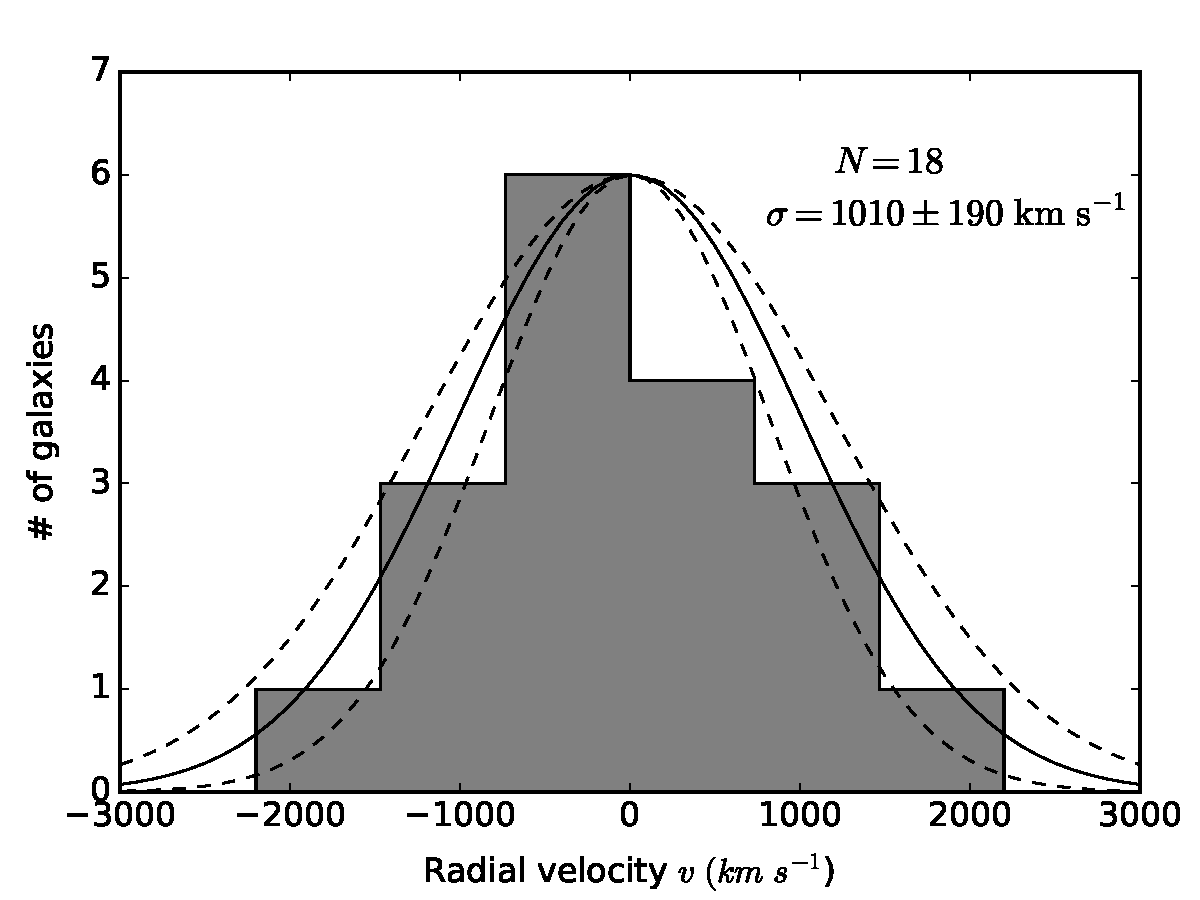
\includegraphics[width=0.6\textwidth]{Chap4/c4f1.pdf}
\caption[Radial velocities of cluster members in \cluster]{Histogram of the radial velocities of the spectroscopically confirmed cluster member galaxies in \cluster\ with respect to the bi-weight center at $z=0.656$. We overplot Gaussians centered on the bi-weight center with widths set to the velocity dispersion (solid line) and its $1\sigma$ errors (dashed lines).}
\label{chap4:fig:vel_hist}
\end{figure}

Figure~\ref{chap4:fig:GMOSspectrum} shows the summed spectrum of \giantarc; we determine a redshift of ($z = 2.4812 \pm0.0005$) from the summed spectrum of four slits placed on the giant arc covering all three images, derived from C~II] and C~III] nebular emission lines. Also visible in the spectra are several low-ionization ISM absorption lines with a systemic redshift of $2.480\pm 0.001$, corresponding to a $\sim100\ \mathrm{km\ s^{-1}}$ outflow.

We targeted two of these lensed galaxies, which were identified as strong lensing constraints (see \S~\ref{chap4:subsec:sec_arcs}), in the \textit{Gemini} Fast Turnaround (FT) program GN-2015A-FT-15 (PI: Johnson, 4.75 hr) using GMOS in long-slit observing mode. Observations were made with the B600 grism and the 1.5"-width long slit, with the slit positioned to target images B1, B2, and several other objects. The final spectra include a total integration time of 9000 s, resulting in spectra covering a wavelength range, $\Delta \lambda \sim 4150-6970$\AA. The spectra of both lensed galaxies include low S/N continuum flux, but no strong features that enable a redshift measurement.

In both the GMOS MOS observations (2011) and FT long-slit, we detect emission from a star-forming galaxy located near B1 (shown in Figure~\ref{chap4:fig:arclabels}). From both observations, we confirm a redshift of $z=0.6447$, based on [OII] 3727\AA\ and Balmer lines for this galaxy, confirming it as a cluster member. Based on its characteristic morphology, this galaxy can be classified as a jellyfish galaxy -- cluster member galaxies with jellyfish-like morphology that exhibit trails of knotted star formation as they pass through the hot intercluster medium and are stripped of their cold gas \citep{Ebeling:2014rf,Suyu:2010xy}.

\begin{figure*}
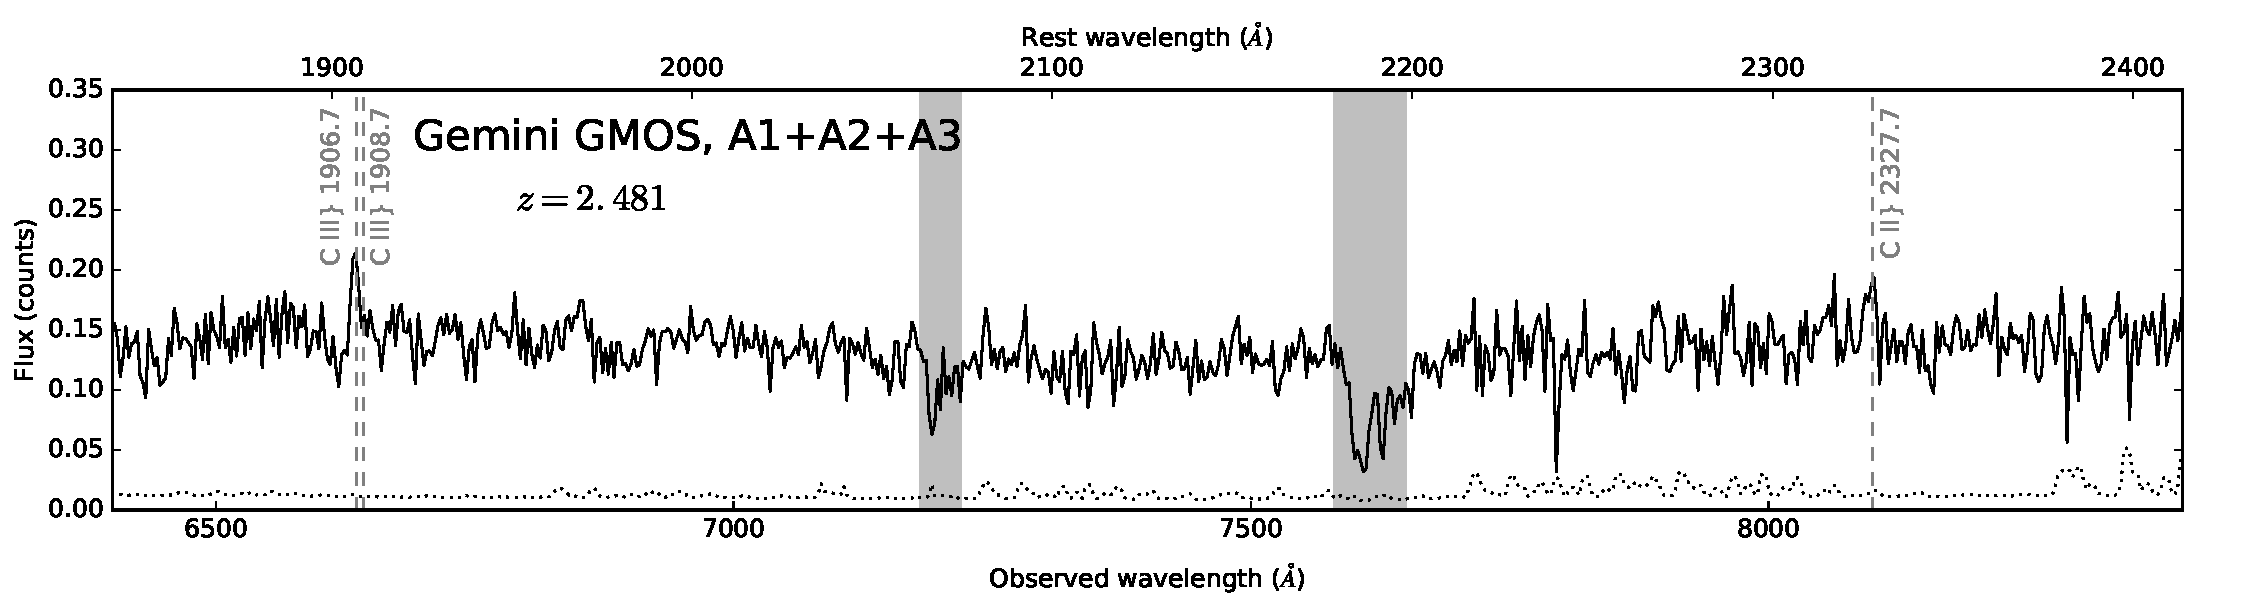
\includegraphics[width=\textwidth]{Chap4/c4f2.pdf}
\caption[GMOS spectrum of \giantarc]{\textit{Gemini} GMOS spectrum of \giantarc, summed from slits placed on all three images (A1, A2, and A3). The dotted line indicates the noise level, and the gray bands indicates part of the spectrum with strong telluric absorption. The vertical gray-dashed lines indicate the locations of rest-frame UV emission lines.}
\label{chap4:fig:GMOSspectrum}
\end{figure*}

\subsection{MMT/Blue Channel Spectrograph}
\giantarc\ was observed on 2015 May 5 with the Blue Channel spectrograph on the 6.5m MMT telescope at Mt. Hopkins, AZ. The spectrograph was configured with a 1.25" wide longslit and the 500 line mm$^{-1}$ grating, resulting in a dispersion of 1.19~\AA\ per pixel, and a spectral resolution, $\delta \lambda \simeq 4.1$~\AA. The data cover a total range in wavelength, $\Delta\lambda = 4000-7150$~\AA. We acquired a total integration time of 6000 s (two 3000 s exposures), and the longslit was aligned along the length of the arc, resulting in emission that extends $\sim$15"\ along the slit. We measure $z = 2.481$ from numerous features that are common in the rest-UV spectra of starburst galaxies, including Ly$\alpha$ emission and absorption from low-ionization species of Si, C, and O (as shown in Figure~\ref{chap4:fig:MMTspectrum}). We note that a spectroscopic redshift for \giantarc\ was reported by \citet{Stark:2013kl} and agrees with our value.

%==================================================================================
%   STRONG LENS MODELING
%==================================================================================
\section{Strong Lensing Analysis of \cluster}
\label{chap4:sec:lensmodel}

\subsection{Previous lensing analysis}
\citet{Oguri:2012bs} use ground-based imaging from the {\it Subaru} telescope to compute strong lensing and weak lensing mass models of \cluster. The strong lens model is severely under-constrained; the primary arc structure could not be resolved, and the source redshift of the primary arc had not yet been spectroscopically confirmed (assumed $z=2\pm1$). Although the secondary arcs we use in our model (which we will discuss in \S~\ref{chap4:subsec:sec_arcs}) are clearly visible in the Subaru imaging, they were not identified or used as constraints in the model. The \citet{Oguri:2012bs} model, with a single mass component, can adequately estimate the mass within the Einstein radius for the fiducial redshift assumed for the redshift of the primary arc. \citet{Oguri:2012bs} note that the weak lensing map suggests the presence of a more complicated mass distribution than indicated from strong lens modeling.

\subsection{Lensing evidence}
With the improved resolution of \hst, we include additional structure within the giant arcs and faint secondary image systems as additional constraints, allowing for a more complex lens model of this cluster. Additionally, the spectroscopic redshifts we have obtained for this cluster help break the mass-sheet degeneracy \citep{Schneider:1995vn} and constrain the slope of the mass distribution.

We identify three unique sources, lensed into a total of 11 images by \cluster, and use the positions of 10 of these images as constraints on the lens model (see Table~\ref{chap4:tab:arcs}). The constraint positions are centered on distinct morphological or chromatic features of the galaxy that are seen in each image. This means that the method is best done by eye rather than a quantitative identifier (i.e. peak emission or barycenter), especially given that the magnifications of these features can vary dramatically from image to image. We include a positional error of 0.3" in the image positions to account for possible small-scale deflections due to structure or galaxy lensing. The positions of the clump features of the giant arc are included as additional constraints. We show the positions of the image constraints in Figure~\ref{chap4:fig:arclabels} and list their coordinates in Table~\ref{chap4:tab:arcs}. 

\begin{figure*}
\centering
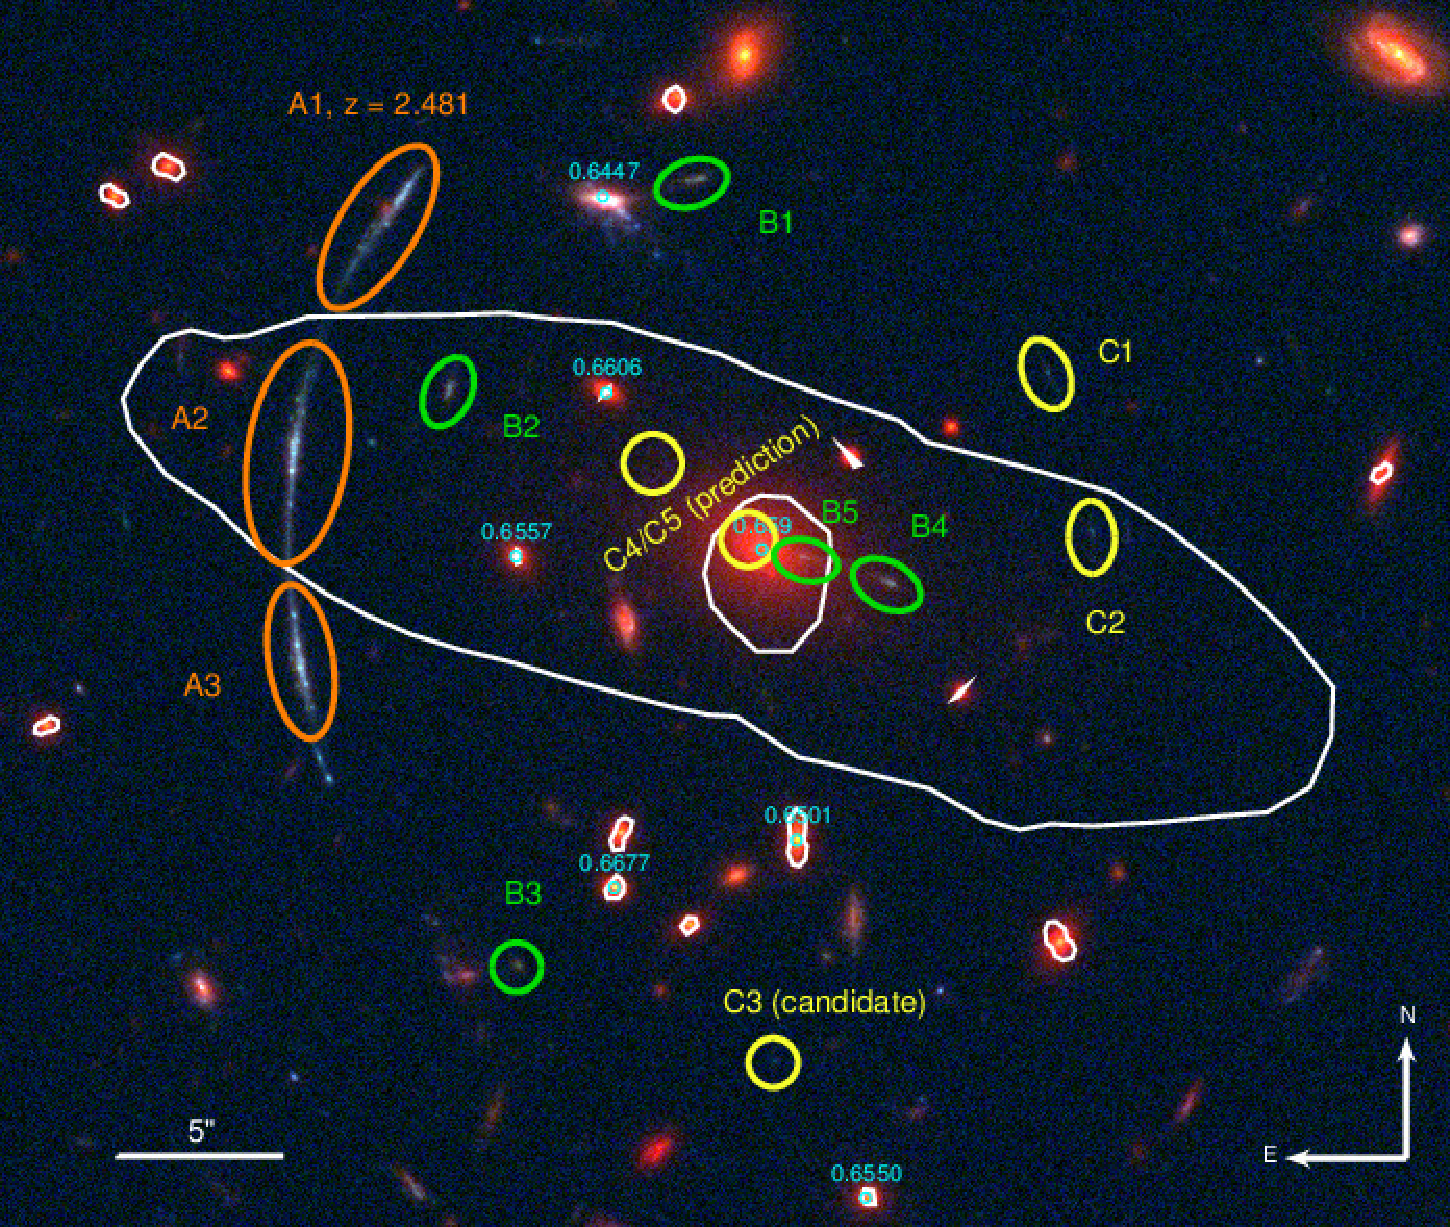
\includegraphics[height=0.3\textheight]{Chap4/c4f3a.pdf}
\includegraphics[height=0.3\textheight]{Chap4/c4f3b.pdf} \\ \vspace{10pt}
\includegraphics[width=0.97\textwidth]{Chap4/c4f3c.pdf}
\caption[\hst\ image and lens model of \cluster]{(Top left) \hst\ WFC3 imaging of \cluster\ in F160W (red), F606W (green), and F390W (blue). Labeled are image systems A, B, and C used in the lens modeling. The redshifts of other objects from Table~\ref{chap4:tab:redshifts} are shown in cyan. The critical curve for $z=\zA$ is shown by the white lines. (Top right) Close up image of the three images of the main arc A and systems D, E, and F; the middle image has been inverted along the N-S direction to match parity with the other two images. The clumps labeled A[a-f] are individual clumps matched across all three images used as constraints in the model. AX and AY are likely part of the lensed galaxy, but lie outside the caustic region and thus are not multiply imaged. Each circle is 0.1" in radius. (Bottom) Images of systems B and C. The dashed circle indicates the center and rms scatter of the predicted images marginalized over all models which predict that image. Each postage stamp cutout is 3" x3".}
\label{chap4:fig:arclabels}
\end{figure*}

\begin{deluxetable}{cccc}
\tablecaption{Identifications of lensed arcs in \cluster}
\tablewidth{0pt}
\tablehead{\colhead{Arc ID} & \colhead{R.A.}       & \colhead{Dec.}      & \colhead{Model$^{b}$} \\
	         \colhead{} &            \colhead{(J2000)} & \colhead{(J2000)} &  \colhead{$z$}}
\startdata
Aa1 & 11:10:19.56 & +64:59:57.88 & 2.481$^{a}$ \\
Aa2 & 11:10:19.96 & +64:59:52.06 &  $\dots$ \\
Aa3 & 11:10:19.92 & +64:59:42.98 &  $\dots$ \\
Ab1 & 11:10:19.51 & +64:59:58.53 & $\dots$ \\
Ab2 & 11:10:20.00 & +64:59:51.16 & $\dots$ \\
Ab3 & 11:10:19.94 & +64:59:43.69 & $\dots$ \\
Ac1 & 11:10:19.48 & +64:59:58.75 & $\dots$ \\
Ac2 & 11:10:20.00 & +64:59:50.81 & $\dots$ \\
Ac3 & 11:10:19.97 & +64:59:44.21 & $\dots$ \\
Ad1 & 11:10:19.47 & +64:59:58.88 & $\dots$ \\
Ad2 & 11:10:20.01 & +64:59:50.54 & $\dots$ \\
Ad3 & 11:10:19.98 & +64:59:44.53 & $\dots$ \\
Ae1 & 11:10:19.45 & +64:59:59.05 & $\dots$ \\
Ae2 & 11:10:20.02 & +64:59:50.27 & $\dots$ \\
Ae3 & 11:10:19.99 & +64:59:44.93 & $\dots$ \\
Af1 & 11:10:19.41 & +64:59:59.46 & $\dots$ \\
Af2 & 11:10:20.03 & +64:59:49.24 & $\dots$ \\
Af3 & 11:10:20.00 & +64:59:45.85 & $\dots$ \\
AX\tablenotemark{c} & 11:10:19.78 & +64:59:40.85 & $\dots$ \\
AY\tablenotemark{c} & 11:10:19.83 & +64:59:41.51 & $\dots$ \\
\hline
B1 & 11:10:19.25 & +64:59:52.61 & $3.79\pm0.17$ \\
B2 & 11:10:18.03 & +64:59:59.27 & $\dots$ \\
B3 & 11:10:18.91 & +64:59:35.06 & $\dots$ \\
B4 & 11:10:17.10 & +64:59:46.80 & $\dots$ \\
B5 & 11:10:17.54 & +64:59:47.63 & $\dots$ \\
\hline
C1 & 11:10:16.34 & +64:59:53.33 & $3.82\pm0.24$ \\
C2 & 11:10:16.14 & +64:59:48.46 & $\dots$ \\
C3\tablenotemark{d} & 11:10:17.674 & +64:59:32.10 & $\dots$ \\
C3\tablenotemark{e} & 11:10:17.775 & +64:59:31.59 & $\dots$ \\
C4\tablenotemark{e} & 11:10:18.257 & +64:59:50.54 & $\dots$ \\
C5\tablenotemark{e} & 11:10:17.796 & +64:59:48.20 & $\dots$ \\
\hline
D1 & 11:10:19.69 & +64:59:57.16 & $2.39\pm0.02$ \\
D2 & 11:10:19.99 & +64:59:52.45 & $\dots$ \\
D3 & 11:10:19.99 & +64:59:43.64 & $\dots$ \\
\hline
E1 & 11:10:19.66 & +64:59:57.51 & $2.37\pm0.02$ \\
E2 & 11:10:20.02 & +64:59:51.89 & $\dots$ \\
E3 & 11:10:20.01 & +64:59:44.17 & $\dots$ \\
\hline
F1 & 11:10:19.62 & +64:59:57.83 & $2.35\pm0.03$ \\
F2 & 11:10:20.03 & +64:59:51.27 & $\dots$ \\
F3 & 11:10:20.02 & +64:59:44.52 &  $\dots$
\enddata
\tablenotetext{a}{Redshift of system A is fixed to the spectroscopic redshift.}
\tablenotetext{b}{The model redshifts are marginalized over all eight lens models.}
\tablenotetext{c}{AX and AY are part of A3, but are not multiply imaged and are not used as constraints in the model.}
\tablenotetext{d}{This galaxy was identified as a possible counter image of system C but was not used as a constraint in the lens model.}
\tablenotetext{e}{Predicted image locations, marginalized over all the models for which an image was predicted.}
\label{chap4:tab:arcs}
\end{deluxetable}


\subsubsection{Primary arc \giantarc}

The primary arc \giantarc\ stretches $\sim$17"\ in length, and is $\sim$15"\ from the BCG. It consists of three images that partially merge together in the image plane (labeled A in Figure~\ref{chap4:fig:arclabels}) with several bright emission knots visible in the \hst\ imaging. The center image, A2, has the highest magnification and most resolved structure. Many of the clumps identified within A2 are unresolved in the other images with lower magnification. With this in mind, we identify six groups of clumps that are multiply imaged, rather than the individual clumps, and use these groupings as model constraints.

There are two bright blobs slightly south of A3 that are likely part of the primary arc (labeled AX and AY in Figure~\ref{chap4:fig:arclabels}). This portion of the galaxy containing these blobs lies outside of the caustic region, and therefore is not multiply imaged.

\begin{figure*}
\includegraphics[width=\textwidth]{Chap4/c4f4.pdf}
\caption[MMT Blue Channel Spectrograph spectrum of \giantarc]{MMT Blue Channel Spectrograph spectrum of \giantarc. The dotted line indicates the noise level, and the gray-solid line is a spectral template of Ly$\alpha$-emitting galaxies with strong absorption features at $z\sim3$ galaxies from \citet{Shapley:2003fk}. The vertical gray-dashed lines indicate the locations of rest-frame UV emission and absorption lines.}
\label{chap4:fig:MMTspectrum}
\end{figure*}

\subsubsection{Identification of multiply imaged galaxies}
\label{chap4:subsec:sec_arcs}
The identification of secondary lensed galaxies is done iteratively, by eye, with the help of the lens model. We identify five sets of multiply imaged secondary arcs (B--F in Figure~\ref{chap4:fig:arclabels} and Table~\ref{chap4:tab:arcs}) in the \hst\ data based on image configuration, morphology, and color. The redshifts of these two background galaxies have not been spectroscopically confirmed, despite our best efforts with \textit{Gemini}/GMOS (see \S~\ref{chap4:sec:specz}), so we leave the redshifts of these secondary arcs as free parameters to be optimized in the lens model. We use estimates of the photometric redshifts (see \S~\ref{chap4:subsec:photoz}) for these galaxies as priors.

Arcs B1 and B2 are tangential arcs located 11.6" north and 10.9" northeast of the BCG, respectively. A third image B3 was predicted and discovered 14.8" southeast of the BCG. We also identified the radial arcs B4 and B5 from color and morphology extending west 4.1" and 1.7" from the center of the BCG.

The faint pair of tangential arcs C1 and C2 are located 10.2" northwest and 10.1" west of the BCG, respectively. We also find a possible candidate for a third image C3 15.8" south of the BCG that matches in color. The location of this candidate is consistent with the image configuration; however, there is a large statistical error on the predicted location of the third image, due to the uncertainty in the redshift of this image system. Also, this image is predicted further from the critical curve than C1 and C2, and has a lower magnification and tangential shear observable by eye, making it difficult to confirm this candidate as the third image by shape. Therefore, we do not include this candidate image as a constraint in the lens modeling.

Near to the primary arc are three bright specks that are slightly different in color than the main arc and are also triply imaged in the same configuration. During the lens modeling process, we found that the positions of these blobs are not as well-reconstructed as the clumps used as constraints within the giant arc when fixed at the same source redshift, suggesting that this may be a separate system at a different redshift. We therefore include these three image systems (D, E, and F) in the lens model, with their redshifts as free parameters.

For all images without spectroscopic redshifts, we use a uniform random prior of $1<z<5$ for the free parameter in the lens model.

The model predicted redshifts for all secondary arcs B--F are listed in Table~\ref{chap4:tab:arcs}. For image system B, the model predicts a much higher redshift than the photometric prediction.

\subsubsection{Photometric Redshifts of Secondary Arcs}
\label{chap4:subsec:photoz}

The photometry of all objects in the \hst\ and {\it Spitzer} imaging was extracted following procedures outlined in \citet{Skelton:2014lr}. Spectral energy distribution (SED) fits and photometric redshifts were computed for all objects using all four \hst\ filters, and the two \textit{Spitzer} IRAC channels using the EAZY redshift code \citep{Brammer:2008uq}. Figure~\ref{chap4:fig:photoz} shows the photometric redshifts of secondary arcs B1, B2, and B3. The redshift probability distribution functions (PDF) support the identification of these images as images of the same galaxy at $z\sim2.7$ ($z_{peak} = 2.68, 2.74, 2.80$, respectively).  At the photometric redshift of image B, this would imply Ly$\alpha$ at $\sim$4500\AA, which was not detected in the GMOS spectrum reported in \S~\ref{chap4:sec:specz}. The lack of such emission does not preclude this photometric redshift, however, as many star-forming galaxies have little or no Ly$\alpha$ emission. There are no other potentially strong emission lines located in the bandpass of the GMOS spectra for this photo-$z$, and so we conclude that the existing spectral data are consistent with the photometric analysis. C1 and C2 were also extracted for photometry for the \hst/UVIS filters but were undetected in Spitzer/IRAC -- four filters were not enough to extract a robust photometric redshift for this image system. Images D, E, and F are all blended with the giant arc, especially in the IR bands, and thus could not be extracted for photometry. Consequently, they do not have photometric redshifts.

\begin{figure*}
\includegraphics[width=\textwidth,trim=0 150 0 150]{Chap4/c4f5.pdf}
\caption[SED and photometric redshift of arcs B1, B2, and B3]{Spectral energy distribution and photometric redshift for arcs B1, B2, and B3. $z_\mathrm{peak}$ is the highest-probability $z$ weighted by $P(z)$: $z_\mathrm{peak} = \int zp(z)dz/\int P(z) dz$. $F_\lambda$ is in units of erg s$^{-1}$ cm$^{-2}$ \AA$^{-1}$.}
\label{chap4:fig:photoz}
\end{figure*}

\subsection{Lens modeling process}
To compute the lens model of \cluster, we used the publicly available software \texttt{LENSTOOL} \citep{Jullo:2007lr}, which utilizes a Markov-Chain Monte Carlo (MCMC) to optimize the parameters of the lensing potential from Bayesian evidence. All of the components of the potential are modeled as pseudo-isothermal elliptical mass distributions \citep[PIEMD;][]{Limousin:2005cr}, which are described by seven parameters: a position $x$ and $y$; an ellipticity $e=(a^2-b^2)/(a^2+b^2)$ where $a$ and $b$ are the semi-major and semi-minor axes, respectively; a position angle $\theta$; a fiducial velocity dispersion $\sigma$; a core radius $r_\mathrm{core}$; and a cut radius $r_\mathrm{cut}$.

The lens modeling is done iteratively. We begin with a set of constraints and our initial guess for the mass distribution within the cluster. Using a preliminary model, we search for new image candidates, which get added as constraints to the model and allow for more free parameters to be included in the next iteration. The early iterations are completed using a source plane optimization. Ideally, optimization should be done in the image plane, as this is where the model constraints lie; however, computation in the source plane is a much faster process, and provides a quick approximation for the lens model. The best-fit models we present here are the final iteration computed under image plane optimization.

\subsubsection{Lens plane mass components}
The total mass distribution of \cluster\ can be characterized by a smooth component encompassing the bulk of the cluster mass, which is perturbed by smaller halos occupied by galaxies. We use a red sequence selection criterion to select cluster member galaxies \citep[i.e.,][]{Gladders:2000kq}. We use the F606W-F105W colors for selecting the galaxies in \cluster\ that best sample the 4000 \AA\ break at the cluster redshift. The galaxies lying on the red sequence are assigned a unique halo with the parameters determined by the \texttt{SExtractor} \citep{Bertin:1996ly} outputs for location, ellipticity, and position angle from the F105W image. We adhere to a light-traces-mass methodology for modeling the perturbing halos, in which brighter galaxies occupy a deeper potential well. The parameters that determine the total mass of the halo, i.e., velocity dispersion $\sigma_0$, core radius $r_\mathrm{core}$, and cut radius $r_\mathrm{cut}$, are scaled by the magnitudes in the F105W band following the relations in \citet{Jullo:2007lr},

\begin{eqnarray}
\sigma_0 &=&  \sigma_0^\star \left(\frac{L}{L^\star}\right)^{1/4} \\
r_\mathrm{core} &=& r_\mathrm{core}^\star  \left(\frac{L}{L^\star}\right)^{1/2} \\
r_\mathrm{cut} &=& r_\mathrm{cut}^\star  \left(\frac{L}{L^\star}\right)^{1/2},
\end{eqnarray}

\noindent where $\sigma_0,r_\mathrm{core},r_\mathrm{cut}$ are the parameters for an $L^\star$ galaxy. These scaling relations translate to a constant mass-to-light ratio for all of the cluster member galaxies. We determine the apparent magnitude of an $L_\star$ galaxy at $z=\zlens$ to be $m_\star=19.9$ in F105W, and we set $\sigma_\star=120\ \mathrm{km\ s^{-1}}$, $r_\mathrm{cut}^\star=30$ kpc, and $r_\mathrm{core}^\star=0.15\ \mathrm{kpc}$. These parameters can also be optimized in the modeling; however, we find that they cannot be constrained easily, as the individual galaxies have a very small and local effect on the lensing potential. Therefore, we choose to fix these parameters and apply deviations from this strict scaling law on individual galaxies when necessary. In this case, we chose to allow the velocity dispersions of the BCG and another galaxy located at R.A. = 11:10:557, decl. = +64:59:58.31 to be free parameters in the model. The BCG affects the slope of the inner mass distribution, and thus the positions of the radial arcs B4/B5. The second galaxy lies almost directly along the line of sight to image A1, and likely will cause small scale--but significant--perturbations to the lensing potential for the clumps in this image. We also use a circular lensing potential for this galaxy, because the flux from A1 interfered with extracting reasonable shape parameters.

We place a massive, cluster-scale halo (also PIEMD) near the location of the BCG. All the parameters are free to optimize, with the exception of the cut radius, which lies far outside the strong lensing regime. It cannot be constrained with the lensing images, so we fix the value to 1500 kpc.

A parametric lens modeling approach is simplistic and appropriate when there are few lensing constraints in a model. However, cluster lensing systems are complicated by non-axisymmetric structure in the dark matter distribution and structures along the line of sight. In the case of \cluster, we find that the basic parametric model is insufficient for reconstructing the lensing, thus necessitating more flexibility. Specifically, models using only cluster-scale halos would, at best, produce an image plane rms of 1.4". We develop a hybrid lens model for this cluster by adding a non-parametric multiscale grid component on top of the parametric cluster- and galaxy-scale halo components described above. We accomplish this via the following methods, developed by \citet{Jullo:2009ij}. We first construct a hexagonal-shaped grid within the lens plane with circular PIEMD halos, or nodes, located on the vertices and at the center, as shown in Figure~\ref{chap4:fig:mass_distribution}. Each node forms an equilateral triangle with its adjacent nodes, and we set the cut radius equal to the side length of the triangle and set $r_\mathrm{cut}=(3/2)r_\mathrm{core}$. This parameterization is arbitrary, but was selected such that each grid halo is not cuspy--rather, each describes a perturbation in a largely smooth mass distribution. We only allow the velocity dispersion of each halo to vary. Thus, each node adds one additional free parameter to the entire lens model. Our over-constrained model allows for many more free parameters, so we allow for the inclusion of more nodes by recursively breaking up the grid into smaller fractal components. Each triangle of nodes split into four equilateral triangles of nodes, each of which is half the size of the original, and every node in the grid is set to the size of the smallest adjacent triangle. This process repeats for every triangle in the grid based on a specified node-breaking criteria and/or a maximum recursion depth. We exclude the nodes centered within a 12" radius from center of the BCG, where the massive cluster halo is located. We give the parameters for forming the multiscale grid in Table~\ref{chap4:tab:grid}. 


\begin{deluxetable}{ccccccccc}
\tablecolumns{9}
\tabletypesize{\scriptsize}
\tablewidth{0pt}
\tablecaption{Multiscale grid parameters}
\tablehead{
	\colhead{} &
	\colhead{Grid} &
	\colhead{Grid} &
	\colhead{Grid} &
	\colhead{Recursion} &
	\colhead{} &
	\colhead{\# of} &
	\colhead{Image} &
	\colhead{Median}
	\\
	\colhead{Size} &
	\colhead{P.A.} &
	\colhead{Shift} &
	\colhead{(")} &
	\colhead{Depth} &
	\colhead{Threshold} &
	\colhead{Nodes} &
	\colhead{Plane} &
	\colhead{Magnification}
	\\
	\colhead{} &
	\colhead{} &
	\colhead{} &
	\colhead{} &
	\colhead{} &
	\colhead{} &
	\colhead{} &
	\colhead{} &
	\colhead{Across Arc}}
\startdata
Model 0 & 30 & -12 & 0 & 2 & 0 & 18 & 0.12 & 18 \\
Model 1 & 30 & -12 & 0 & 3 & 5 & 23 & 0.11 & 35 \\
Model 2 & 30 & -12 & 2.5 & 3 & 5 & 23 & 0.10 & 36 \\
Model 3 & 30 & -42 & 0 & 2 & 0 & 18 & 0.12 & 26 \\
Model 4 & 40 & -12 & 0 & 2 & 0 & 18 & 0.11 & 24 \\
Model 5 & 40 & -12 & 0 & 3 & 5 & 21 & 0.12 & 42 \\
Model 6 & 40 & -12 & 2.5 & 3 & 5 & 29 & 0.12 & 28 \\
Model 7 & 40 & -42 & 0 & 2 & 0 & 18 & 0.11 & 17
\enddata
\tablecomments{The grid size is the separation of the nodes and radius of the nodes at the first level of recursion depth. The position angle is the orientation of the major axis measured north of east ($-12^\circ$ aligns the major axis of the grid with the semi-major axis of the BCG). The grid shift is the shift of the center of the grid along the orientation of its major axis in the direction toward the middle image of arc A. The threshold is the number of constraints in each node required to recursively break that node into smaller nodes. The image plane rms is the rms scatter between the observed and predicted positions of the images used as constraints -- because all models use the same constraints, image plane rms serves as a measurement for goodness of fit.}
\label{chap4:tab:grid}
\end{deluxetable}


\begin{figure*}
\center
\includegraphics[width=\textwidth]{Chap4/c4f6.pdf}
\caption[Surface mass density of \cluster\ lens model]{Surface mass density of each lens model. The circles show where each node of the multi scale grid is centered, with radius equal to the cut radius of that node. Overlaid on grid for reference are the locations for arcs A (red), B (green), and C (blue). All offsets are given with respect to the center of the BCG.}
\label{chap4:fig:mass_distribution}
\end{figure*}

Because our primary objective in adding more free parameters to the lens model is an accurate source magnification and reconstruction, we base our node-breaking criteria on the local density of constraints. For each triangle of nodes, we count the number of constraints within a circle connecting each of the three nodes, and the triangle is broken down into more nodes if the number density within the circle is above a set threshold. We present eight models using a variety of grid parameters -- node size, node-breaking criteria, recursion depth, grid center, and grid orientation. Each model produces similar masses and magnification. The image plane root mean square (rms) of all the models is $\sim0.11"$.

We estimate the uncertainties in the model parameters, magnifications, and masses from a suite of simulated models produced during the MCMC. We select models with the lowest image plane rms. Our model selection was chosen such that models span roughly the $1\sigma$ spread in values for the free parameters, which are well-constrained and have roughly Gaussian posterior probability distributions. This cut includes $\sim$100 models, and thus provides an adequate sampling of the parameter space around the best-fit model. Therefore, it can be used to estimate the statistical errors in the lens modeling.

\subsection{Mass distribution}

The surface mass distribution for each of the eight lens model multiscale grid configurations is shown in Figure~\ref{chap4:fig:mass_distribution}. The shape of the mass distribution beyond the location of the lensing constraints follows the design of the grid; however, the overall profile is well-constrained by the lensing. This is especially true on the eastern side of the cluster, in the vicinity of arc A, where the density of lensing constraints is high. We compute the integrated mass profile within radius $r$ of the galaxy cluster out to a radius of 500 kpc in Figure~\ref{chap4:fig:mass_profile} for each of the eight models. The mass profiles of all models are the same within their statistical errors; they have especially good agreement around 100 kpc, approximately the projected radius of the strong lensing arcs used as constraints in the model (i.e., Einstein radius). Despite how much the surface mass density can change in regions when different parameterizations for the mass distribution are used, the total mass remains fairly robust.

Marginalizing over all eight models, we compute aperture masses centered on the BCG $M(r<250\ \mathrm{kpc}) = 1.7\pm0.1\times10^{14}\ \msol$ and $M(r<500\ \mathrm{kpc}) = 3.1\pm0.2\times10^{14}\ \msol$. The area enclosed within the $z=\zA$ critical curve is $A(<\mathrm{crit}) = 0.0983\pm0.003\ \square'$, enclosing a mass of $M(<\mathrm{crit}) = 3.3\pm0.1\times10^{13}\ \msol$. The effective Einstein radius for the giant arc is $\theta_\mathrm{E} = \sqrt{A(<\mathrm{crit})/\pi} = 10.6\pm0.2"$.

Although the models produce low statistical errors on the mass, we warn that the slope of the mass distribution is highly prone to systematic errors. Our model only contains one spectroscopic redshift, and we are unable to accurately break the mass sheet degeneracy \citep{Schneider:1995vn}. This degeneracy can be broken using multiple source planes, i.e., multiple systems of different source redshift. Although we have included secondary arcs at different source redshifts than the main arc in our model, their model-derived redshifts are inconsistent with photometric redshifts. Our eight lens models produce similar slopes for the mass distribution because they each derive similar redshifts for the secondary arcs. However, because the redshifts may be incorrect (see \S~\ref{chap4:subsec:model_redshifts}), the mass sheet degeneracy has been artificially broken; therefore, the mass slopes are likely incorrect. However, the mass enclosed within the critical curve remains the most accurate measurement of the mass.

We estimate the dynamical mass from the radial velocities of cluster member galaxies (\S\ref{chap4:sec:specz}) using the $\sigma_{DM}-M_{200}$ scaling relation from \citet{Evrard:2008uo}. The velocity dispersion we measure yields a dynamical mass of $M_{200} = 8.1^{+7.5}_{-5.8}\times10^{14}\ \msol$ for \cluster. With this relation, however, we are assuming that strong lensing clusters are not biased in mass. Strong lensing clusters are more likely to be oriented with the principle axis aligned along the line of sight \citep{Hennawi:2007ek}, resulting in a 19\% bias in cluster mass.

\begin{figure}
\centering
\includegraphics[width=0.7\textwidth]{Chap4/c4f7.pdf}
\caption[Integrated mass profile of \cluster]{We plot the integrated mass profile within radius $r$ of the galaxy cluster \cluster\ for each of the eight lens models. The shaded region indicates the $1\sigma$ uncertainty range in the mass. The dashed lines indicate the locations of the effective Einstein radius at $z=\zA$ and the radius of the giant arc. All models are in good agreement and converge at the Einstein radius, which corresponds roughly to the typical projected radius of the multiple images used as constraints in the lens models.}
\label{chap4:fig:mass_profile}
\end{figure}

The \citet{Oguri:2012bs} lens model is represented by a single elliptical NFW profile with $M_{vir}=2.26^{+2.41}_{-0.96}\times10^{14}\ \msol$ and concentration parameter $c=22.39^{+17.42}_{-15.70}$. For a circular NFW profile, this yields $M(r<250\ \mathrm{kpc}) = 0.8^{+0.9}_{-0.5}\times10^{14}\ \msol$ and $M(r<500\ \mathrm{kpc}) = 1.3^{+1.3}_{-0.7}\times10^{14}\ \msol$. The two models are in agreement at smaller radii, as both are built from strong lensing. Our model, with more strong lensing constraints and a spectroscopic redshift of the main arc, has a higher-fidelity mass estimate in this region. However, the lack of agreement at larger radii spawns from the lack of weak lensing constraints in our model -- we measure the mass distribution less accurately on the outer regions of the cluster than \citet{Oguri:2012bs}.

\subsection{Magnification}
\label{chap4:subsec:magnification}

We measure the magnification of the arc by combining all magnification maps across the eight lens models. In Figure~\ref{chap4:fig:magmap}, we include the median magnification of each pixel in the image plane at $z=\zA$ across all eight lens model realizations, weighted by the errors estimated from the MCMC chain. We find that the magnification across the middle image A2 is $\sim5-10\times$, with a typical statistical error of 20\% for any given pixel. The median and mean pixel count-weighted magnification across the middle image of the arc are $\sim8$ and $\sim9$, respectively.

\begin{figure*}
\includegraphics[width=\textwidth]{Chap4/c4f8.pdf}
\caption[Magnification map of \cluster]{The weighted median magnification map for a source at $z=\zA$ stacked from all eight different lens models (left) and the corresponding uncertainty in magnification marginalized across all eight models (right). The locations of the multiple images are shown by the black ovals.}
\label{chap4:fig:magmap}
\end{figure*}

\subsection{Predicted images for system C}
All of our lens models predict a counter-image for C1 and C2 in the vicinity of our candidate image C3. The barycenter of the image predictions from all eight models is listed in Table~\ref{chap4:tab:arcs}, with an rms scatter of 1.60". This location is only 0.82" away from our candidate image C3, which is well within the scatter of the predictions.

Half of our models (0,1,4,7) predict a set of radial images, C4 and C5, in the center of the cluster opposite of the radial images B4 and B5. The barycenter of the image predictions for the four models that predict these central images are listed in Table~\ref{chap4:tab:arcs}. The predictions for images C4 and C5 are located 4.3" and 0.5" away from the center of the BCG, with a scatter of 0.9" and 0.8", respectively. We are unable to identify any likely candidates for these radial arcs; however, this does not rule out these models. These central images are predicted to be demagnified by a factor of $\sim4-10$, and would be hidden by the light from the BCG; therefore, if they exist, we likely would not see them in this data.

\subsection{Model-predicted redshifts versus photometric redshifts}
\label{chap4:subsec:model_redshifts}
Our lens models predict higher redshifts for the image system B than the photometric redshifts of B1/B2/B3 suggest, by more than 5$\sigma$, indicating a high tension between the models and observations. Similarly, the model redshifts of $z\sim3.8$ would lead to a non-detection in F390W, which indicates that the redshift for system C may also be incorrect. Based on observations, the model redshifts are likely incorrect. However, in lens modeling, redshift of the source is not the relevant quantity, but rather the ratio of angular diameter distances between lens and source $d_\mathrm{ls}$ in relation to observer and source $d_\mathrm{s}$. This lensing ratio, $d_\mathrm{ls}/d_\mathrm{s}$, scales the deflection angle, which is what is used to determine the locations of multiple images in the lens modeling process; redshift of a source is a secondary measurement from lens modeling based on choice of cosmological parameters. For system B, a difference in model versus photometric redshifts of $z\sim3.8$ and $z\sim2.7$ equates to only a $\sim10\%$ difference in $d_\mathrm{ls}/d_\mathrm{s}$. This value for the error can be propagated into uncertainties in mass and magnification of sources, as the lensing ratio is used to scale all of the quantities that go into those calculations. Additionally, the \texttt{Lenstool} software has a tendency to bias unknown redshifts used as free parameters to systematically higher values, as investigated in \citet{Johnson:2016rt}, which may help to explain the redshift tension in our models.

%==================================================================================
%   Forward Modeling
%==================================================================================
\section{Source plane reconstruction for \giantarc}
\label{chap4:sec:clump_model}
Gravitational lensing allows us to measure the substructure of galaxies with much higher resolution than field galaxies. Our lens model translates between the observed image plane clump and their physical size and position in the source plane. Naively, the physical size of the clumps can be determined by measuring the image plane area and dividing by the factor of the magnification. This method breaks down quickly when considering unresolved structures, as the true lensed shape of the clump is lost when the lensed image is convolved with the instrument PSF. A more accurate reconstruction of source structure that is at the diffraction limit of the telescope when lensed requires a way to disentangle the effects of nonuniform magnification across the image and instrument PSF.

To this end, we have created a forward modeling technique to reconstruct the sizes of the star-formation clumps in the source plane. The clumps are modeled in the source plane and then ray-traced to the image plane, convolved with the instrument PSF, and compared to the observed data.

Forward modeling techniques, although computationally costly, have been shown in previous lensing studies to be quite useful in accurately reconstructing the source. These techniques have been used frequently with lower-resolution data of sub-millimeter galaxies \citep{,MacKenzie:2014kx,Dessauges-Zavadsky:2016fj}. \citet{Fu:2012yq} reconstruct a parameterized source accounting for very different PSFs/beams from optical to sub-millimeter. With the onset of higher-resolution sub-millimeter facilities, such as the \textit{Atacama Millimeter/Sub-millimeter Array}, these forward-modeling techniques have evolved to allow for a full reconstruction of the source in the complex \textit{uv} plane from interferometric data \citep{Hezaveh:2013vn,Hezaveh:2016ys}.

\subsection{Initial image plane Gaussian decomposition}
Because we are focusing on the clumps, we first perform a Gaussian decomposition of the main arc in order to separate the clumpy structure from the diffuse background. We combine the F606W and F390W to create a higher signal-to-noise detection image. We use GALFIT \citep{Peng:2010qy} to create a parameterized model of the lensed galaxy in the image plane. Two-dimensional Gaussian components are placed in the image plane at the locations of bright clumps and are fit simultaneously to the data.  The best-fit model of the arc is then subtracted from the data to reveal more clumps, which are added to the model and are fit again. This process is done iteratively until the resulting residuals are consistent with the background noise. The final model in F606W+F390W is then used as a template to separately fit each of the F606W and F390W images.

\begin{figure*}
\center
\includegraphics[scale=0.7,resolution=300,trim=0 50 0 50]{Chap4/c4f9.pdf}
\caption[GALFIT decomposition of \giantarc]{GALFIT clump decomposition in F606W (top) and F390W (bottom) imaging. (A) \hst\ imaging of the middle image of \giantarc\ in the image plane. (B) The complete GALFIT model of the middle image of the arc. (C) Clump component of panel B. (D) Smooth component of panel B. (E) Residual of the clump+smooth GALFIT model and the data in units of rms noise.}
\label{chap4:fig:galfit_model}
\end{figure*}

We separate the Gaussian components used to create these models into two sets. The clump model consists of bright blobs with sizes roughly a few times that of the \hst\ PSF in the image plane, which will translate to sizes $<100$ pc in the source plane. The smooth model has lower surface brightness and covers nearly the entire length of the arc in the image plane. These models are shown in Figure~\ref{chap4:fig:galfit_model}.

\subsection{Source plane clump model}
We model each clump in the source plane as a two-dimensional Gaussian on a grid of 0.003" pixels (to allow for $\sim10\times$ magnification), then ray trace the light distribution back to the image plane via custom ray-tracing code written in Python. We use a Bayesian approach to model the clump parameters, allowing for both parameter space exploration and model comparison. We use the publicly available Python package \texttt{emcee} to perform an affine-invariant sampling of model parameter space \citep{Foreman-Mackey:2013rf}. This sampling provides us with an estimate for the posterior PDF

\begin{equation}
\mathrm{Pr}(\vec\theta | D,M) = \frac{\mathrm{Pr}(D | \vec\theta, M)\ \mathrm{Pr}(\vec\theta | M)}{\mathrm{Pr}(D | M)}
\end{equation}

\noindent for a selection of parameters $\vec\theta$, given the design of the source plane model $M$ and the observed data in the image plane $D$. Here, $\mathrm{Pr}(D | \vec\theta, M)$ is the prior PDF of a $\vec\theta$ for a given model $M$; $\mathrm{Pr}(D | M)$ is the evidence, which normalizes the posterior PDF and accounts for the model complexity; $\mathrm{Pr}(D | \vec\theta, M)$ is the likelihood function of getting the observation $D$, given a source plane model $M$ with parameters $\vec\theta$. According to Bayesian theory, the model that is the best fit will maximize the posterior PDF; one with high likelihood, but is consistent with priors and is more simplistic. Because the evidence is constant for a given M, for this analysis, we will only maximize the non-normalized posterior PDF.

We define the likelihood function of our source plane model as

\begin{equation}
\mathrm{Pr}(D | \vec\theta, M) = \prod_{i=1}^{N} \frac{1}{\sigma\sqrt{2\pi}}\mathrm{Exp}\left[-\frac{\chi^2}{2} \right],
\end{equation}

\noindent where $N$ is the number of pixels in the image plane over the region encompassing the giant arc (see below for definition). The contribution to the overall $\chi^2$ from each image plane pixel is

\begin{equation}
\chi^2  = \sum_{i=0}^{N}\frac{1}{\sigma^2}[I_\mathrm{d}(x_i)-I'_\mathrm{s}(x_i | \vec\theta)]^2,
\end{equation}

\noindent where $I_\mathrm{d}$ is the surface brightness of the observed data at image plane position $x$, and 

\begin{equation}
I'_\mathrm{s}(\vec x | \vec\theta) = I_\mathrm{s}(\vec x | \vec\theta) \ast f(\vec x)
\end{equation}

\noindent is the surface brightness of the model $M$ in the image plane. Here, $I_\mathrm{s}$ is the source plane model surface brightness, ray-traced to the image plane position $x$, which is then convolved in the image plane with the empirical PSF of the instrument $f(x)$.

An empirical PSF is computed for each filter, using data from the entire SGAS \hst\ program GO13003. We select stars in each cluster frame, coadded after subtracting for background features and nearby objects, following \citet{Skelton:2014lr}. We then fit a Gaussian profile to the PSF, and use this as our kernel for smoothing the model to the resolution of \hst.

Because our empirical PSF was averaged over many different epochs of HST observations, it is likely not an exact match to the PSF at the time and position on the detector of the 
SDSS J1110+6459 observations.  According to the WFC3 handbook,\footnote{http://www.stsci.edu/hst/wfc3/documents/handbooks/currentIHB/c06\_uvis07.html} the PSF at 0.4 $\mu$m can vary with breathing by up to 3\%.  Variation of the PSF spatially across the detector can be comparable to the spatial variation.\footnote{http://www.stsci.edu/hst/wfc3/documents/ISRs/WFC3-2013-13.pdf} Therefore, we include runs of our MCMC that account for a $\pm5\%$ and $\pm10\%$ error in the size of the Gaussian convolution kernel when measuring sizes and fluxes of the clumps. We find no trend in changes of size and flux for the different PSF sizes used, only an overall increase in the statistical errors.

For mapping the image plane to source plane, we use the deflection matrices from Model~2, which has the lowest image plane rms and is close to the median magnification per pixel for the middle image A2 across all eight models. Model~2 produces magnifications across A2 that are neither extremely high nor low compared to the other models. We optimize two parameters for each clump: flux and size. We tested shape parameters (i.e., ellipticity and position angle), but found these parameters could not be constrained for even the brightest and most resolved clumps and thus were not included in the optimization. The clumps are centered on the source plane position that maps to the peak in brightness of that clump in the image plane.  All parameters are assigned uniform random priors.

The best-fit clump parameters are given in Table~\ref{chap4:tab:clump_parameters}. We estimate the errors on each parameter from the posterior probability distributions in the MCMC. Figure~\ref{chap4:fig:source_plane_model} shows the best-fit model of the source plane clumps in both the image plane and source plane for the central image. Figure~\ref{chap4:fig:full_arc_model} shows the clumps ray-traced to all three images of the arc. In this figure, we have removed the clumps corresponding to arcs D, E, and F. The model predicts these images to be at slightly different redshifts than the main arc and will be offset from where they are in A1 and A3. To avoid confusing these clumps with those from \giantarc, we have removed them from the source plane model used in the ray-tracing.

\begin{landscape}
\begin{deluxetable}{ccccccccccc}
\tabletypesize{\footnotesize}
\tablecolumns{7}
\tablewidth{0pt}
\tablecaption{\giantarc\ source plane clump parameters}
\tablehead{\colhead{Clump} & 
                  \colhead{$\Delta$R.A} &
                  \colhead{$\Delta$Decl.} &
                  \colhead{$m_\mathrm{F606W}$} &
                  \colhead{$m_\mathrm{F390W}$} &
                  \colhead{Size} &
                  \colhead{Lensing PSF} &
                  \colhead{Size} &
                  \colhead{Lensing PSF} &
                  \colhead{Magnification} \\[4pt]
	         \colhead{ID} &
	         \colhead{(kpc)} &
	         \colhead{(kpc)} &
	         \colhead{(mag)} &
	         \colhead{(mag)} &
	         \colhead{F606W (pc)} &
	         \colhead{F606W (pc)} &
	         \colhead{F390W (pc)} &
	         \colhead{F390W (pc)} &
	         \colhead{}}
\startdata
D\tablenotemark{*} & 1.08 & -1.71 & 31.83 ($31.76^{+0.10}_{-0.11}$) & 32.81 ($32.54^{+0.15}_{-0.13}$) & 33.6 ($36.6^{+3.2}_{-3.3}$) & $26.8^{+3.1}_{-2.3}$ & 62.3 ($61.5^{+2.6}_{-2.6}$) & $22.1^{+5.4}_{-2.5}$ & 8.5 [5.6-14.2] \\[4pt]
E\tablenotemark{*} & 0.95 & -0.62 & 31.82 ($31.75^{+0.09}_{-0.16}$) & 32.84 ($32.87^{+0.19}_{-0.16}$) & 30.1 ($33.2^{+1.7}_{-1.9}$) & $25.3^{+2.7}_{-1.8}$ & 31.7 ($33.4^{+1.9}_{-2.2}$) & $20.0^{+4.6}_{-2.1}$ & 8.5 [5.5-14.1] \\[4pt]
F\tablenotemark{*} & 0.58 & 0.52 & 32.21 ($32.11^{+0.09}_{-0.14}$) & 33.18 ($32.98^{+0.21}_{-0.18}$) & 30.9 ($32.1^{+2.7}_{-1.7}$) & $27.5^{+3.7}_{-2.8}$ & 36.4 ($37.5^{+2.9}_{-3.0}$) & $18.7^{+6.6}_{-3.4}$ & 9.0 [5.7-14.6] \\[4pt]
3 & -0.50 & 2.01 & 30.44 ($30.45^{+0.04}_{-0.07}$) & 30.75 ($30.73^{+0.08}_{-0.07}$) & 30.5 ($31.8^{+3.5}_{-1.6}$) & $27.9^{+1.8}_{-3.3}$ & 22.0 ($22.1^{+1.8}_{-1.7}$) & $22.6^{+4.3}_{-3.5}$ & 10.2 [6.3-15.6] \\[4pt]
4 & -0.89 & 2.78 & 32.31 ($32.18^{+0.12}_{-0.14}$) & 33.28 ($33.45^{+0.16}_{-0.15}$) & 28.9 ($31.8^{+2.1}_{-1.4}$) & $28.4^{+1.7}_{-2.1}$ & 35.9 ($34.8^{+2.0}_{-1.9}$) & $22.8^{+8.6}_{-4.9}$ & 12.0 [7.3-17.5] \\[4pt]
5 & -0.86 & 3.38 & 31.17 ($31.12^{+0.05}_{-0.11}$) & 31.39 ($31.41^{+0.07}_{-0.07}$) & 32.3 ($33.6^{+1.2}_{-1.2}$) & $27.6^{+2.2}_{-1.6}$ & 32.7 ($34.7^{+2.3}_{-2.1}$) & $24.0^{+8.8}_{-5.2}$ & 15.3 [9.2-21.6] \\[4pt]
6 & -0.88 & 3.93 & 32.32 ($32.30^{+0.15}_{-0.12}$) & 32.31 ($32.65^{+0.16}_{-0.16}$) & 30.7 ($34.8^{+4.2}_{-3.5}$) & $29.1^{+2.6}_{-2.3}$ & 40.3 ($35.8^{+2.5}_{-2.4}$) & $24.3^{+4.2}_{-4.8}$ & 25.0 [14.5-34.7] \\[4pt]
7 & -0.26 & 1.11 & 30.92 ($30.91^{+0.09}_{-0.08}$) & 31.38 ($31.38^{+0.08}_{-0.08}$) & 31.2 ($33.6^{+2.0}_{-2.5}$) & $26.3^{+2.1}_{-3.6}$ & 36.6 ($36.8^{+4.2}_{-3.6}$) & $21.5^{+15.0}_{-4.5}$ & 9.0 [5.6-14.2] \\[4pt]
8 & 0.10 & 0.58 & 31.14 ($31.17^{+0.06}_{-0.07}$) & 31.59 ($31.60^{+0.08}_{-0.08}$) & 29.8 ($32.5^{+2.7}_{-2.1}$) & $27.0^{+2.1}_{-2.9}$ & 43.6 ($38.1^{+4.2}_{-3.8}$) & $20.9^{+5.2}_{-3.6}$ & 8.8 [5.5-14.1] \\[4pt]
9 & 0.00 & 0.00 & 32.28 ($32.23^{+0.09}_{-0.14}$) & 32.35 ($32.22^{+0.12}_{-0.11}$) & 33.1 ($35.0^{+2.6}_{-2.3}$) & $27.7^{+1.8}_{-2.9}$ & 56.9 ($50.3^{+4.2}_{-4.2}$) & $22.9^{+7.4}_{-4.2}$ & 8.2 [5.2-13.3] \\[4pt]
10 & 0.37 & -0.33 & 32.50 ($32.55^{+0.20}_{-0.15}$) & 32.80 ($32.93^{+0.21}_{-0.16}$) & 32.6 ($37.0^{+4.8}_{-3.8}$) & $28.0^{+1.8}_{-1.6}$ & 52.3 ($56.3^{+3.6}_{-3.8}$) & $21.8^{+3.7}_{-3.9}$ & 8.3 [5.3-13.6] \\[4pt]
11 & 0.04 & -0.59 & 32.75 ($32.58^{+0.13}_{-0.13}$) & 33.09 ($32.93^{+0.19}_{-0.16}$) & 48.7 ($42.2^{+4.4}_{-5.3}$) & $28.8^{+1.7}_{-3.5}$ & 38.3 ($40.0^{+3.3}_{-3.3}$) & $22.3^{+6.6}_{-5.3}$ & 7.9 [5.1-13.0] \\[4pt]
12 & 0.15 & -1.28 & 31.90 ($31.89^{+0.08}_{-0.11}$) & 32.83 ($32.84^{+0.18}_{-0.16}$) & 32.9 ($34.4^{+1.7}_{-2.0}$) & $25.7^{+4.3}_{-2.6}$ & 19.9 ($19.6^{+1.9}_{-1.8}$) & $22.3^{+7.6}_{-5.6}$ & 7.9 [5.1-13.0] \\[4pt]
13 & 0.62 & -1.18 & 32.34 ($32.37^{+0.13}_{-0.12}$) & 33.28 ($33.26^{+0.26}_{-0.22}$) & 42.7 ($39.6^{+2.7}_{-3.0}$) & $27.7^{+2.5}_{-3.7}$ & 45.0 ($38.5^{+4.2}_{-4.2}$) & $18.3^{+3.7}_{-4.1}$ & 8.2 [5.3-13.5] \\[4pt]
14 & -0.12 & 0.27 & 32.13 ($32.14^{+0.10}_{-0.11}$) & 32.58 ($32.67^{+0.16}_{-0.14}$) & 33.6 ($34.7^{+2.7}_{-2.9}$) & $25.8^{+2.5}_{-1.7}$ & 36.5 ($38.8^{+2.8}_{-2.9}$) & $20.3^{+9.6}_{-4.4}$ & 8.3 [5.3-13.5] \\[4pt]
15 & -0.30 & 0.39 & 31.72 ($31.72^{+0.15}_{-0.10}$) & 32.14 ($32.08^{+0.10}_{-0.10}$) & 35.9 ($34.2^{+1.7}_{-2.1}$) & $26.9^{+3.4}_{-1.4}$ & 30.4 ($33.8^{+2.7}_{-2.7}$) & $19.8^{+7.4}_{-3.7}$ & 8.3 [5.2-13.3] \\[4pt]
16 & -0.40 & 1.55 & 33.11 ($32.73^{+0.29}_{-0.24}$) & 33.24 ($33.05^{+0.22}_{-0.19}$) & 41.2 ($43.5^{+4.1}_{-4.8}$) & $26.9^{+2.3}_{-2.0}$ & 45.6 ($42.4^{+4.1}_{-4.1}$) & $20.1^{+3.3}_{-2.5}$ & 9.5 [5.9-14.8] \\[4pt]
17 & -0.04 & 0.83 & 31.46 ($31.42^{+0.06}_{-0.06}$) & 31.63 ($31.69^{+0.11}_{-0.09}$) & 42.5 ($42.9^{+4.8}_{-4.4}$) & $26.8^{+2.1}_{-2.2}$ & 63.3 ($54.2^{+5.6}_{-5.0}$) & $23.7^{+6.2}_{-4.2}$ & 8.9 [5.6-14.2] \\[4pt]
18 & -0.83 & 1.85 & 32.92 ($32.88^{+0.24}_{-0.23}$) & 32.75 ($32.97^{+0.22}_{-0.18}$) & 37.2 ($42.2^{+3.6}_{-4.5}$) & $25.7^{+2.2}_{-2.9}$ & 38.7 ($39.0^{+3.1}_{-3.1}$) & $20.4^{+6.8}_{-3.9}$ & 9.6 [5.9-14.6] \\[4pt]
19 & 0.90 & -2.46 & 32.95 ($32.87^{+0.19}_{-0.18}$) & 32.88 ($32.59^{+0.15}_{-0.14}$) & 32.5 ($33.9^{+1.8}_{-2.1}$) & $26.3^{+2.4}_{-2.4}$ & 41.2 ($40.1^{+2.7}_{-3.0}$) & $21.6^{+8.0}_{-5.1}$ & 9.1 [6.0-15.2] \\[4pt]
20 & 1.14 & -2.95 & 32.30 ($32.14^{+0.14}_{-0.17}$) & 33.20 ($33.06^{+0.24}_{-0.21}$) & 44.1 ($37.2^{+4.9}_{-6.2}$) & $27.7^{+1.9}_{-2.6}$ & 30.9 ($30.2^{+3.9}_{-3.7}$) & $19.7^{+5.1}_{-3.1}$ & 10.3 [6.9-17.3] \\[4pt]
21 & 1.16 & -3.12 & 32.39 ($32.21^{+0.12}_{-0.16}$) & 32.54 ($32.70^{+0.17}_{-0.15}$) & 30.7 ($32.9^{+3.2}_{-2.3}$) & $26.8^{+1.9}_{-2.2}$ & 38.2 ($31.1^{+3.1}_{-2.9}$) & $20.2^{+5.3}_{-3.9}$ & 10.8 [7.3-18.3] \\[4pt]
22 & 1.02 & -2.71 & 32.88 ($32.60^{+0.22}_{-0.22}$) & 32.90 ($32.92^{+0.21}_{-0.17}$) & 39.0 ($47.6^{+4.4}_{-7.3}$) & $26.9^{+2.9}_{-3.3}$ & 51.3 ($42.2^{+4.5}_{-4.4}$) & $24.0^{+3.5}_{-5.4}$ & 9.5 [6.4-16.0] \\[4pt]
23 & 1.35 & -0.50 & 33.83 ($33.44^{+0.54}_{-0.31}$) & 33.49 ($33.43^{+0.26}_{-0.23}$) & 37.4 ($35.4^{+2.0}_{-2.1}$) & $28.7^{+1.8}_{-1.9}$ & 16.8 ($16.4^{+2.3}_{-2.2}$) & $23.1^{+4.7}_{-7.7}$ & 8.9 [5.8-14.7] \\[4pt]
24 & 0.68 & -1.82 & 32.93 ($32.73^{+0.26}_{-0.18}$) & 33.99 ($33.75^{+0.42}_{-0.31}$) & 45.2 ($42.0^{+3.6}_{-2.8}$) & $27.4^{+2.5}_{-1.5}$ & 40.9 ($40.8^{+4.7}_{-5.1}$) & $24.3^{+5.5}_{-6.8}$ & 8.3 [5.5-13.8] \\[4pt]
25 & -1.30 & 2.91 & 33.13 ($33.02^{+0.25}_{-0.24}$) & 33.96 ($33.38^{+0.35}_{-0.27}$) & 49.3 ($46.3^{+4.5}_{-4.0}$) & $27.8^{+1.4}_{-2.0}$ & 27.5 ($35.4^{+4.9}_{-4.8}$) & $24.1^{+4.1}_{-3.4}$ & 11.8 [7.2-17.2] \\[4pt]
26 & 1.50 & -2.67 & 33.22 ($32.80^{+0.21}_{-0.22}$) & 33.88 ($33.51^{+0.32}_{-0.29}$) & 32.5 ($33.4^{+2.6}_{-2.5}$) & $25.2^{+2.1}_{-1.3}$ & 18.2 ($21.9^{+4.9}_{-4.4}$) & $25.4^{+5.9}_{-8.3}$ & 10.0 [6.7-16.8]
\enddata
\tablenotetext{*}{These ``clumps" correspond to sources D, E, and F in the lens model, and are not part of the galaxy. We report their sizes and fluxes at the redshift of the main arc, $z=\zA$.}
\tablecomments{Column (1) clump Identifier; (2) and (3) relative R.A and decl., in kpc at arc redshift, relative to clump \#9; (4) F606W magnitude of clumps in the source plane; (5) same as (4), for F390W; (6) source plane size (HWHM) of the clumps in F606W, in parsecs; (7) size of lensing PSF in the source plane in F606W, in parsecs; (8) and (9) same as (6) and (7), respectively, for F390W; (10) clump magnification. For columns 4, 5, 6, 8, we report the best-fit parameter first, and in parenthesis show the median and $1\sigma$ errors on the parameter from the MCMC. For columns 7 and 9, we report the  median and $1\sigma$ errors on the parameter from the MCMC. The last column shows the median magnification; in brackets, the full range of magnifications is given for all eight lens models.}
\label{chap4:tab:clump_parameters}
\end{deluxetable}
\end{landscape}

\begin{figure*}
\centering
\includegraphics[width=0.9\textwidth]{Chap4/c4f10.pdf}
\caption[Source plane model of SFR clumps in \giantarc]{Left panel: model of clumps in the source plane. Note: the middle image of the galaxy has negative parity in declination; for display purposes the y-axis has been flipped to match the orientation of galaxy in the image plane. Panel A: the source plane model from the left panel, ray-traced to the image plane and convolved with the \hst\ PSF. Panel B: the clump decomposition model (also Panel B from Figure~\ref{chap4:fig:galfit_model} with added noise). The inset shows the source plane model (left panel), scaled to its true angular size with respect to its magnified image. Panel C: residual of source plane model and clump decomposition, in units of rms noise.}
\label{chap4:fig:source_plane_model}
\end{figure*}

\begin{figure}
\centering
\includegraphics[width=0.5\textwidth,trim={1cm 2.5cm 0.6cm 1cm},clip]{Chap4/c4f11.pdf}
\caption[Ray-traced model of \giantarc\ in the image plane]{Left panel: model of clumps ray-traced to the image plane in all three images of the giant arc. Right panel: \hst\ data of the entire giant arc. Both panels are coadded F606W and F390W. The stretch of the scaling is square root.}
\label{chap4:fig:full_arc_model}
\end{figure}

\subsection{Completeness Analysis}
We expect our results to be affected by observational biases, in that fainter and smaller clumps are less likely to be detected. Given that the sizes of star-forming regions in the local universe follow a power law, we expect there to be many more of these difficult to detect clumps in galaxies \citep{Kennicutt:1989fk}; thus, our models are incomplete.

To understand our completeness limits, we run simulations determining the efficiency of detection of clumps, based on their size and flux. We create a set of 1000 lensed galaxies similar in design to \giantarc, using new parameters for the simulated clumps. At each image plane position of the clumps in our model of \giantarc, we assign a new position perturbed by a few pixels. We ray-trace all new positions for the simulated clumps to the source plane, where we place fake clumps. The parameters for 18 (2/3) of those fake clumps are drawn randomly from the list of best-fit parameters of the detected clumps, with replacement (i.e., the parameters listed in Table~\ref{chap4:tab:clump_parameters}). For the remaining 9 (1/3) clumps, we select parameters randomly to have a $m_\mathrm{F606W}=30-37$ and $r=1-40$ pc. These ranges were chosen to cover the parameter space where we expect to measure a significant change in the efficiency function for detecting a clump. For simplicity, we assign all clumps the same color $m_\mathrm{F390W}-m_\mathrm{F606W}=0.36$, which is the typical color of the clumps derived from the source plane measurements from the forward modeling MCMC. All the clumps have the same size in both F606W and F390W. We then ray-trace the source plane models for both F390W and F606W of the fake clumps back to the image plane, convolve with their respective PSFs, and coadd the images. We then add the model of the F606W+F390W smooth component to the fake clumps and add realistic noise.

Next, we run our clump-finding algorithm on the simulated lensed galaxies, where we create a GALFIT model of the entire galaxy, clumps and smooth component. The only inputs used for the algorithm are the new image plane positions of the fake clumps. Added to the GALFIT model are three locations that are not included in the simulated galaxy, which we select randomly from three of the exact positions of the clumps chosen. The purpose of these three additional components is to determine the typical background level of the clumps at those positions. GALFIT will attempt to fit a clump at those locations, even though there is no assigned flux in the source plane model that maps to that position. The output magnitude of that false clump tells us the position-dependent threshold for whether or not a clump near that position can be detected. This threshold is influenced by many factors: sky background, magnification, the brightness of the smooth component at that position, and nearby clumps that may overlap. We define the background level at each position to be the median magnitude of the false clumps measured by GALFIT. We define a simulated clump as ``detected" if its GALFIT magnitude is brighter than one standard deviation above the background level at the position where it was measured. All the clumps were detected well above this limit.

Our simulations reveal that clump detection depends strongly on the flux of the clump in F606W, and is independent of size for clumps that are larger than 10 pc in the image plane. As we will show below, our resolution limit is roughly 20 pc. Therefore, we combine the efficiency measurements across all clumps larger than 10 pc, and fit the efficiency as a function of magnitude using

\begin{equation}
\eta(m) = \frac{N_0}{1 + \exp[(m-m_{0.5})/s]}.
\label{chap4:eqn:efficiency}
\end{equation}

\noindent The model fit and parameters are shown in Figure~\ref{chap4:fig:efficiency_fits}. Our 80\% completeness limit is 33.2 mag.

Although our detection efficiency depends only on clump magnitude, our model is still limited in the size of clumps measured, due to resolution limits. To determine the size limit, we create a model of \giantarc\ in the image plane, where we have replaced each clump with the instrument PSF, the highest resolution we can achieve for a given clump at that location within the galaxy. Each of these PSFs are given a uniform brightness that roughly matches the average measured brightness of all clumps in the image plane. We apply our forward modeling algorithm to this model, to determine the size of the lensing PSF in the source plane; i.e., the smallest size we can measure in the source plane, given its magnification and the instrument PSF. The sizes of the lensing PSFs for the clumps in F390W and F606W are given in Table~\ref{chap4:tab:clump_parameters}, ranging from 24 to 31 parsecs for F606W and from 17 to 30 parsecs in F390W.

\begin{figure}
\centering
\includegraphics[width=0.8\textwidth]{Chap4/c4f12.pdf}
\caption[Empirical detection efficiency of clumps in \giantarc]{Model fits to the empirical efficiency for clumps larger than 10 pc, as a function of clump magnitude. The best-fit parameters to (\ref{chap4:eqn:efficiency}) for each size bin are shown in the upper right-hand corner.}
\label{chap4:fig:efficiency_fits}
\end{figure}

\section{Summary}
\label{chap4:sec:summary}

\subsection{Hybridization of lens modeling}
In this paper, we have demonstrated that a multiscale grid model for the mass distribution, which was first implemented for Abell 1689 by \citet{Jullo:2009ij}, can be applied to smaller lensing clusters like \cluster. We attempted to model \cluster\ with a traditional parametric lens model, and found that it was impossible to robustly reconstruct the source plane surface brightness of \giantarc\ robustly in all three images. Adding the additional flexibility of a multiscale grid allows for a model that accurately reconstructs the source galaxy. Quantitatively, the image plane rms decreased from 1.4" in the parametric model to typically 0.1" in the multiscale grid models.

\subsection{Advantages and disadvantages of forward modeling versus traditional ray-traced source plane reconstruction}
\label{chap4:subsec:method_comparison}

Our forward modeling methodology has allowed us to obtain unprecedented physical resolution of galactic structure of a galaxy at $z=\zA$ in the source plane. Field galaxies (i.e., unlensed) were typically resolved down to one kiloparsec scales in surveys with \hst. Previous studies of lensed galaxies have uncovered resolution limits on the order of a few hundred parsecs \citep{Jones:2010uq,Livermore:2012fk,Swinbank:2012jk,Wisnioski:2012qf,Livermore:2015ve}. Our methodology effectively allows us to deconvolve the source plane structure with the lensing PSF, which is the effect of applying the instrument PSF in the image plane to a galaxy that is magnified asymmetrically. The magnification $\mu$ of an object is defined as the ratio of image plane area to source plane area; therefore, if the lensing shear is isotropic, the ratio of the image plane radius and source plane radii of a circular object should be equal to the square root of the magnification, $\sqrt\mu$. In cases where the shear is not isotropic, as is typically the case in giant arcs like \giantarc\ (where the galaxy is lensed tangentially around the center of the lensing potential), we expect the ratio between the radius in the image plane and the semi-minor (semi-major) axis in the source plane to be slightly larger (smaller) than $\sqrt\mu$. In the image plane, the smallest resolvable angular scale is determined by the instrument PSF. The \hst\ F606W PSF has a Gaussian width of 0.033" (FWHM=0.078"); thus, the smallest resolvable physical scale in the source plane would correspond to roughly $0.033"/\sqrt\mu$. For a source a $z=\zA$ and $\mu=12$ (median magnification of the clumps), this scale corresponds to roughly 77 pc. Therefore, we expect that ray tracing \giantarc\ in the usual manner would not be able to measure sizes smaller than about 60-70 pc. However, our results reveal that \giantarc\ does not have clumps larger than 40 pc. 

We directly compare our forward modeling results to the traditional ray-tracing methodology. We create a source plane model of the clumps by ray-tracing the GALFIT image plane model of the clumps in F606W back to the source plane, using methods similar to \citet{Sharon:2012ly}. We then measure the size of each clump in the source plane by fitting a two-dimensional Gaussian centered on the position of each clump in the model, with four free parameters: amplitude, semi-major axis, semi-minor axis, and position angle. Our Gaussian fits to our ray traced clumps in \giantarc\ have a median semi-minor (semi-major) axis fit of 86.9 (143) pc, which is over twice the value of the largest clump we measure using our forward modeling technique. We find that, for individual clumps, the highest resolution achieved by ray tracing (i.e., the semi-minor axis) is $3.5\pm1.6$ times larger than that measured through forward modeling. Our methods allow us to obtain higher resolution isotropically, rather than along the axis of the clump that is tangential to the direction of the shear. We measure a typical axis ratio (semi-major axis/semi-minor axis) to be $1.8\pm0.8$, usually with this tending toward higher values for higher-magnification clumps. Therefore, the semi-major axis of the clumps will still be measured as $5.6\pm1.8$ times larger than the forward modeling measurement.

The results show that forward modeling produces a much higher resolution view of source plane structure compared to traditional ray tracing, especially when measuring structure smaller than the size of the ray-traced PSF in the source plane. However, what traditional ray tracing lacks in spatial resolution, it gains over forward modeling in computational speed. Ray-tracing pixels from an image plane grid to a source plane grid takes a matter of minutes and needs only be done once for a single image of a source; the same solution to the lensing equation can be applied to any image plane surface brightness model created on the same grid of pixels. The forward modeling method takes advantage of the same procedure as ray-tracing does, in that it maintains the same solution for mapping source plane to image plane pixels; however, it needs to be run many times for full parameter space exploration. This technique simplified the surface brightness profile of the source galaxy with two-parameter Gaussian profiles representing each of 27 clumps. A single model can be produced in under 2 s, but the 300,000 models produced in the MCMC take roughly 16 hr to complete (on four cores with a 2.20 GHz processor).

The speed of forward modeling is thus limited in how many free parameters are included in the source plane model. To model the source galaxy in more detail would require more parameters, or ideally, a non-parametric approach where each the brightness of each source plane pixel is its own free parameter in the model. This non-parametric approach can be developed for future work regarding high-resolution studies of lensed galaxies, either by increasing the computational resources beyond those we used in this work, or repurposing adaptive mesh refinement codes to work for lensing.

\subsection{Magnification uncertainties}
The systematic uncertainty on magnification is the most significant uncertainty in measuring the sizes of the lensed clumps in the source plane. As we found in \S~\ref{chap4:subsec:magnification}, the eight models that we produced for this cluster produce median magnifications across the giant arc \giantarc\ ranging from 18 to 36. A higher or lower typical magnification of a model will shift the size distribution of the clumps by roughly a factor of $1/\sqrt{\mu}$. Therefore, a $\sim60\%$ systematic error on magnification translates to a systematic error of $\sim20\%$ on the source plane sizes of the clumps.

%==================================================================================
%   CONCLUSIONS
%==================================================================================
\section{Conclusion}
\label{chap4:sec:conclusion}

We have used the power of \hst\ imaging and strong gravitational lensing to resolve structure on $<100$ pc scales in a lensed galaxy \giantarc\ at $z=\zA$. The mass distribution of the lensing galaxy cluster \cluster\ at $z=\zlens$ was mapped through a hybrid parametric-non parametric lens modeling technique developed specifically for this investigation. We measured spectroscopic redshift for the main arc and cluster member galaxies, which fixes the lensing geometry of the lens equation and provides a more robust estimate for the surface mass density of the cluster. We find that our strong lensing mass estimate is consistent with a dynamical mass estimate measured from the velocity dispersion of the cluster, as well as previous strong+weak lensing models of this cluster performed without spectroscopic data. From the lensing mass, we determine the deflection tensors that provide the translation between the observations of the lensed galaxy made in the image plane and the true surface brightness distribution of the galaxy in the source plane. We model the central, most highly magnified image of the lensed galaxy with GALFIT, decomposing the clumpy component from the smooth distribution of light, and implement a forward modeling technique to measure the sizes and luminosities of the clumps in the source plane. Our completeness analysis shows that we have detected the vast majority of clumps brighter than 33.2 mag in F606W, and have achieved a typical resolution limit of $\sim$20-30 pc (magnification dependent) across the galaxy.

Our study has demonstrated the usefulness of gravitational telescopes for understanding the structure of galaxies during the peak epoch of universal star formation. Exciting as these studies are, current sample sizes of lensed galaxies are too small to generalize to the entire galaxy population at high redshift. Many giant arcs have been discovered through various surveys; the bottleneck of the analysis remains in developing accurate lens models to robustly reconstruct the galaxies in the source plane. Strong lens modeling is far from an automated process; identifying multiple images, measuring spectroscopic errors, and computing the models requires considerable human effort for each lensing cluster. Additionally, these studies require a full analysis of the systematic errors of the modeling process. Strong lensing systematics are currently being studied in the context of the most massive, most effective lenses, i.e., the Frontier Fields \citep[see][]{Meneghetti:2016xe,Johnson:2016rt}; however, the parameter space relevant to this work remains unexplored: low-mass clusters with few multiple images and even fewer spectroscopic redshifts. Although the most well-studied lensing clusters are among the most massive in the universe, the majority of clusters that produce giant arcs are those that are most common: low-mass clusters. These clusters have smaller lensing cross-sections, and therefore will typically lens fewer multiple image systems that can be used as constraints. Thus, it is imperative that lensing systematics be studied in small cluster systems, so that future studies similar to this work on \giantarc\ to have the highest accuracy.

We will enter deeper discussions on the scientific impact of the clump sizes and brightnesses we have measured in this paper in future work. Paper II will show how high magnification is necessary to reveal structure within galaxies at high redshift, as we will show in a comparison of our resolved model of \giantarc\ compared to our model of this galaxy, mocked to the resolution and depth of the CANDELS survey. In Paper III, we will analyze the size and brightness distributions of the clumps, and compare our results for the surface density of star formation with those of other galaxies across cosmic time.

\vspace{24pt}
Support for program \# 13003 was provided by NASA through a grant from the Space Telescope Science Institute, which is operated by the Association of Universities for Research in Astronomy, Inc., under NASA contract NAS 5-26555. We thank the Spitzer Science Center for prompt, detailed, expert advice on reducing our data. K.E.W. gratefully acknowledges support by NASA through Hubble Fellowship grant \#HF2-51368 awarded by the Space Telescope Science Institute, which is operated for NASA by the Association of Universities for Research in Astronomy, Inc., under contract NAS 5-26555.


\chapter{Star Formation at $z=2.481$ in the Lensed Galaxy SDSS J1110$+$6459: Star Formation down to 30~parsec scales}
\label{chap:clumps}
\section{Preface}

This chapter has been adapted from a letter of the same title in the Astrophysical Journal Letters, Volume 843, page L21 \citep{Johnson:2017uq}, with co-authors Jane R.~Rigby, Keren Sharon, Michael D.~Gladders, Michael Florian, Matthew B.~Bayliss, Eva Wuyts, Katherine E.~Whitaker, Rachael Livermore, and Katherine T. Murray. It is fully reproduced here under the non-exclusive rights of publication granted by the American Astronomical Society to the paper authors.

This project is based off of the results found in Chapter~4 and \citet{Johnson:2017fj}. I created the last three figures and provided the files for creating the first figure. I wrote some of the introduction and the figure captions. JRR wrote much of the discussion section. The both of us co-wrote the methods section.


%==================================================================================
%   TITLE, AUTHORS, AFFILIATIONS
%==================================================================================
%\author{Traci L. Johnson\altaffilmark{1}, Jane R.~Rigby\altaffilmark{2}, Keren Sharon\altaffilmark{1}, 
%Michael D.~Gladders\altaffilmark{3,4}, Michael Florian\altaffilmark{2}, Matthew B.~Bayliss\altaffilmark{5}, 
%Eva Wuyts\altaffilmark{6}, Katherine E.~Whitaker\altaffilmark{7,8}$^\dagger$, 
%Rachael Livermore$^{10}$, \& Katherine T. Murray\altaffilmark{9}}

%==================================================================================
%   ABSTRACT
%==================================================================================
\section{Abstract}
We present measurements of the surface density of star formation, 
the star-forming clump luminosity function, and the clump size distribution function, 
for the lensed galaxy \giantarc\ at a redshift of $z=$\zA .
The physical size scales that we probe, radii \rangeofscales, 
are considerably smaller scales  than have yet been studied at these redshifts.  
The star formation surface density we find within these small clumps is consistent with
surface densities measured previously for other lensed galaxies at similar redshift.  
Twenty-two percent of the rest-frame ultraviolet light in this lensed galaxy arises
from small clumps,  with $r<$100~pc. 
Within the range of overlap, the clump luminosity function  measured for this 
lensed galaxy is remarkably similar to those of $z\sim0$ galaxies.  
In this galaxy, star-forming regions smaller than 100~pc---physical scales not 
usually resolved  at these redshifts by current  telescopes---are important locations 
of star formation in the distant universe.  If this galaxy is representative, 
this may contradict the theoretical picture in which the critical size scale for star
formation in the distant universe is of order 1 kiloparsec.
Instead, our results suggest that current telescopes have not yet resolved the critical size scales of star-forming activity 
in galaxies over most of cosmic time.  

%==================================================================================
%   INTRODUCTION
%==================================================================================
%\section{Introduction}\label{sec:intro}

Deep field surveys with \textit{The Hubble Space Telescope}  (\hst) 
have revealed that more than half of star-forming galaxies 
at $1< z < 3$ exhibit clumpy morphologies in the rest-frame 
ultraviolet \citep{Shibuya:2016wt}.  Motivated by these  results over 
the past decade,  a theoretical picture has emerged in which 
1~kiloparsec is a critical size scale, perhaps {\it the} critical scale, for 
star formation in the distant universe 
\citep{Elmegreen:2005xy, Elmegreen:2007qv, Elmegreen:2009nr, Forster-Schreiber:2011sf, 
Guo:2011rm, Guo:2015zl}.  
In that scenario, such large clumps arise from gravitational instabilities in gas-rich disks 
\citep{Toomre:1964fr, Noguchi:1999vf, Genzel:2011ys},
and are thought to highlight spots where cold gas may have accreted onto the disk 
\citep{Keres:2005yq, Dekel:2006qf, Brooks:2009jk}.

In this scenario, star formation at early times occurred in complexes that are preferentially much larger 
than in galaxies in the local universe.  
However, this hypothesis is hard to test, as structures much smaller than 1~kpc cannot 
normally be resolved by current telescopes.  
Even \hst\ is unable to  resolve star formation  at these redshifts on spatial 
scales smaller than about 500~pc, due to the diffraction limit.  
As a result,  the clumpy, 
complex morphology of star formation that is known to occur 
in nearby galaxies is normally inaccessible at the epoch when 
most of the stars in the universe were formed (see review by \citealt{Madau:2014qd}.) 

A way to overcome current observational limits and test this theoretical picture is to use
gravitational lensing by natural telescopes \citep{Einstein:1936cl, Zwicky:1937yq}.
Distant galaxies can be strongly gravitationally lensed into giant arcs that are highly magnified.  
To date, this technique has been exploited for dozens of lensed galaxies at 
$z>1$, which have revealed the importance of star-forming clumps with spatial 
scales down to several hundreds parsecs (e.g.~\citealt{Livermore:2012fk, Jones:2010uq}.)

Our \textit{HST} program (GO 13003) observed 
$\approx 70$ giant arcs behind 
37 lensing clusters that were selected by the 
Sloan Giant Arcs Survey (SGAS; Gladders et al., in prep).  
SGAS is a survey for strongly lensed, highly magnified galaxies selected from 
the Sloan Digital Sky Survey (SDSS).  
Galaxy clusters were selected from the SDSS photometric catalog using the 
red sequence method \citep{Gladders:2000kq}; cluster fields were 
then systematically searched for giant arcs.
Candidates lenses were confirmed, then followed up with an extensive
ground- and space-based observational campaign.
A full description of the SGAS-HST program will appear in Sharon et al.\ (2018, in prep). 
This Letter concerns one target from that larger program, \giantarc, hereafter \arcname.

In this Letter, we use the gravitationally lensed galaxy 
arcname\ to provide a 
remarkably sharp view into how stars form in the distant universe.
The giant arc, at redshift $z=2.481$, is comprised of three images of the galaxy with a 
total magnification of \totalmagnification\  (Figure~\ref{chap5:fig:HSTimage}.) 

High spatial resolution, provided by rest-frame UV imaging with \textit{HST} plus 
lensing magnification,  and combined with a new forward-modelling technique 
(Johnson et al. 2017, hereafter Paper~I),
reveals that the morphology of star formation is extremely clumpy.  
There is also a spatially extended component with rest-frame UV color indistinguishable 
from that of the clumps  (Rigby et al.\ 2017, hereafter Paper~II).
\arcname\ is forming stars at a rate of  $8.5$$^{+8}_{-0.4}$~$^{+4}_{-2}$~M$_{\odot}$ yr$^{-1}$ 
(uncertainties from SED fitting, and from the magnification uncertainty; Paper~II.)
The galaxy's stellar mass is $\log M^* = 9.24$~M$_\odot$, with associated uncertainties of 
 $^{+0.11}_{-0.15}$  from SED fitting and 
$^{+0.08}_{-0.12}$ from the magnification uncertainty (Paper~II).
This stellar mass is comparable to the median $\log M^* = 9.4$~M$_\odot$ for the 
lensed sample with H$\alpha$ measurements from \citet{Livermore:2015ve}.
The peak contribution to the global star formation rate density at $z\sim2$ comes 
from galaxies with about ten times higher stellar mass, with galaxies of the stellar 
mass of \arcname\ contributing three to five times less \citep{Leja:2015si}.
Were \arcname\ not lensed, \hst\ would measure it to 
be forming stars in a smooth, exponential disk, with a size and structure that is 
typical for galaxies of its redshift and stellar mass (Paper~II).

Paper~I produced a lens model of 
galaxy cluster \cluster, and also 
developed a novel forward--modeling technique that reconstructs 
the sizes and brightnesses of the clumps in the source plane.  This method has 
advantages over traditional ray-tracing techniques in that it is able 
to effectively deconvolve the source from the ``lensing point spread function'' (PSF),
which results as a combination of the telescope/instrumental PSF and
asymmetric shear of lensing.  
Paper~I used extensive simulations to determine the 
detectability of clumps as a function of intrinsic physical size and luminosity.  

Accordingly, with star-forming clumps detected with sizes down to \smallestscale, 
\arcname\ provides the sharpest view of a $z\sim2$ galaxy yet obtained.
In this Letter, %using the lensing model and source-plane reconstructions of Paper~I, 
we analyze the distribution of star formation surface density within \arcname, 
as well as the clump luminosity function and size distribution function.
In doing so, we probe, for the first time, 
star formation at cosmic noon on spatial scales well below 100~pc.

\section{Methods}\label{sec:methods}
This Letter builds on the results from Paper~I and Paper~II.
In Paper~I, we constructed a source-plane model of the unlensed image
of each of the emission clumps in \arcname, 
modeling each clump as a Gaussian 
parameterized by its half-width-at-half-maximum (HWHM) size 
and its intrinsic flux normalization.
Paper~I also provides an estimate of the  
$80\%$ flux completeness limit of 
\fluxcompleteness\ (the magnitude at which artificially injected clumps were recovered 
$80\%$ of the time), and quantifies the 
smallest spatial scales that can be distinguished in the source plane
due to lensing PSF.
The constraints on the stellar populations that are used in this
Letter were derived in Paper~II,
from a spectral energy distribution analysis. 

In this work, we estimate the star formation rates (SFR) of the clumps in
\arcname\ as follows.  
To obtain the intrinsic rest-frame ultraviolet flux density, we integrate 
the 2D Gaussian that best fits the F606W source-plane reconstruction of each clump, 
and divide by ($1+z$) to correct for bandwidth compression.  
We use Equation~1 of \citet{Kennicutt:1998ee}
to estimate the SFR, 
with a correction factor of 1.8 to convert the initial mass function from Salpeter to Chabrier.
In calculating SFRs, we assumed no extinction, 
given the constraints of $A_v = 0.0$--0.2 derived from fitting the spectral 
energy distribution (Paper~II).

In the following sections, we compare our results to
measurements of SFR inferred from Paschen~$\alpha$ luminosities
of H~II regions in nearby galaxies \citep{Liu:2013qy}.
To convert the Paschen~$\alpha$ inferred rate, we use Equation 2 of
\citet{Kennicutt:1998ee}, with the same correction factor for the initial mass function.
%correction factor of 1.8 to convert the IMF to Chabrier.
We take \HaParatio\ as the intrinsic H$\alpha$/Pa$\alpha$ ratio, 
which assumes Case B recombination, $T=10^4$~K, and $n_e =100$~cm$^{-3}$ .

We assume a flat cosmology with $\Omega_M = 0.3$, $\Omega_{\Lambda} = 0.7$, 
and $H_0 = 70$~km s$^{-1}$~Mpc$^{-1}$.
In this cosmology, an angular size of 1" 
corresponds to an angular diameter distance of 8.085~kpc at the 
redshift of \arcname\ at $z=$\zA . 

\section{Results}\label{sec:results}
The physical properties of individual star-forming clumps in
\arcname\ can be compared to measurements of other galaxies from the
literature, by examining the size--SFR space, and the
distributions of sizes and SFRs of individual clumps or galaxies. 

In Figure~\ref{chap5:fig:surfacedensity}, we consider the surface density of star formation
in the individual clumps in \arcname.
This plot, developed by \citet{Livermore:2012fk} and \citet{Livermore:2015ve}, 
is a way to parameterize the intensity of star formation.
We compare to literature measurements of galaxies at
a range of redshifts, from $z=0$ to $z=5$, both lensed and unlensed, 
mostly compiled by  \citet{Livermore:2015ve}.

For \arcname, the SFR is inferred from the rest-frame ultraviolet
(F606W filter) as explained in \S~\ref{sec:methods}.
In the comparison samples, the star formation rates for most of the
measurements come from H$\alpha$, 
with the exception of the \citet{Swinbank:2007wj} and
\citet{Swinbank:2009lk} samples, 
which use the [O II]~3727, 3729~\AA\ doublet. 
Local measurements come from the SINGS galaxy sample \citep{Kennicutt:2003xq} and 
the DYNAMO $z\sim 0.1$ sample \citep{Fisher:2017tk}.  
Relative to \citet{Livermore:2015ve}, we have changed how the $z=0$ SINGS galaxies 
are plotted; since \citet{Livermore:2015ve} did not probe as small
clumps sizes as we do here, they had binned each galaxy and applied a surface brightness threshold,  
to match the spatial resolution and depth of their sample of lensed galaxies.
Here, we re-measure the SINGS galaxies without binning.  % Email from Rachael 13 July 2016
We note that of the $z\sim 1$ galaxies, the % 
samples of  \citet{Swinbank:2012jk} and %WiggleZ 
\citet{Wisnioski:2012qf} samples are not gravitationally lensed, whereas 
the other distant galaxy samples are lensed. 

In Figures~\ref{chap5:fig:sfr_distrib} and~\ref{chap5:fig:size_distrib}, we plot the differential luminosity
function of clumps in \arcname, and differential distribution of clump
sizes, respectively, and compare them to measurements from the nearby universe \citep{Liu:2013qy}.

We measure the SFR surface density at $z\sim2.5$ for star-forming clumps 
with radii below 100 pc.  To the best of our knowledge, this is the first time 
that size scales well below 100~pc have been measured in the distant universe. 
In Figure~\ref{chap5:fig:surfacedensity}, the clumps from \arcname\ 
follow the $1.5<z<3$ line of constant star formation surface density 
that has been measured \citep{Livermore:2015ve},  for larger size scales, at this epoch.
Thus, we confirm previous results \citep{Livermore:2012fk, Livermore:2015ve} 
that star-forming clumps in bright lensed
$z\sim2$ galaxies have high star formation surface density, 
considerably higher than observed in the  $z\sim 0$ 
SINGS sample \citep{Kennicutt:2003xq} comparison sample, and 
comparable to those observed in the $z\sim 0$ \citet{Fisher:2017tk} sample.

Twenty-two percent of the rest-frame ultraviolet light of \arcname\ arises from 
more than twenty star-forming clumps, with measured sizes of  \rangeofscales. 
The largest clump we measure is \largestclump.  

The clump luminosity function shows a similar slope 
and normalization to that observed for Pa$\alpha$ at $z\sim0$.  
Figure~\ref{chap5:fig:sfr_distrib} shows reasonably good agreement, 
in the range of overlap, 
between the luminosity function we measure for \arcname\ and that measured
using Pa$\alpha$ for nearby galaxies by \citet{Liu:2013qy}.  A detailed comparison is
premature given that we are only examining one galaxy, but this result
indicates the value of expanding such comparisons to larger samples of lensed galaxies.

 The distribution function of clump size (Figure~\ref{chap5:fig:size_distrib})
is dominated by smaller clumps 
($r\sim 30$--40~pc), and shows a notable lack of the larger ($40<r<100$~pc) clumps 
that dominate the size distribution seen for P$\alpha$ at 
$z\sim0$ \citep{Liu:2013qy}.  
Simulations (Paper~I) indicate that the smallest size scale we can recover in \arcname\ is 
about \smallestscale.
Stochasticity is doubtless a factor at the larger sizes, given that we are only examining one galaxy,
and prevents any comparison of the slope with the power law observed at larger sizes
by \citet{Liu:2013qy}.
 
\section{Discussion}
Previous measurements \citep{Livermore:2012fk, Livermore:2015ve}   
of the evolution of star formation surface density  over cosmic time
shown in Figure~\ref{chap5:fig:surfacedensity} 
have been interpreted as evidence that galaxies
become more extreme with increasing redshift, evolving toward 
higher star formation surface densities.  However, there are important selection effects at work.
The lensed galaxies plotted in Figure~\ref{chap5:fig:surfacedensity} are generally of high surface brightness.
Since lensing preserves surface brightness, and surface brightness dimming scales as $(1+z)^4$, 
we would expect only regions of high surface brightness to be observable in these galaxies \citep{Calvi:2014bm}.
Indeed,  Figure~\ref{chap5:fig:surfacedensity} shows that for \arcname, 
we could not recover clumps with the typical surface brightnesses of 
$r<100$~pc clumps from SINGS, but we could
recover clumps with typical surface brightnesses of the $z\sim 0.1$ DYNAMO 
sample \citep{Fisher:2017tk}.

Given this, we cannot rule out a picture in which the star formation in \arcname\ 
is even clumpier than we can measure, and that the clumps we detect are only the 
brightest with highest surface brightness.  This would explain why 
the spatially extended (``diffuse'') component shows the same 
rest-frame UV color as the clumps (Paper~II).

The previous use of SINGS \citep{Kennicutt:2003xq} as the 
$z=0$ comparison sample may have exaggerated 
the contrast between $z\sim0$ and $z>1$, 
since the SINGS sample, by selection, does not include vigorously star-forming galaxies. 
By contrast, Figure~\ref{chap5:fig:surfacedensity} shows that 
the clumps from the $z\sim 0.1$ DYNAMO galaxies \citep{Fisher:2017tk} 
have star formation surface densities
an order of magnitude higher than those of the SINGS galaxies, and
indeed just as high as those seen at $z \sim 2$.

In the future, it will be possible with \textit{JWST} to make apples-to-apples 
comparisons between the most luminous clumps in nearby luminous infrared galaxies, 
and the most luminous clumps in lensed galaxies, 
for example using  H$\alpha$ integral field unit spectroscopy from NIRSpec, 
or Paschen~$\alpha$ integral field spectroscopy from MIRI.

Nevertheless, the measurements presented in this Letter indicate that at the
epoch of galaxy assembly,  star formation occurred on much smaller 
spatial scales than has been previously assumed.  
Such spatial scales have not been 
previously accessed in the distant universe, as without lensing
magnification, they fall below the resolution limit of present day telescopes.

The lensed galaxy \arcname\ at $z=$\zA\  is forming stars at a rate of 
$8.5$$^{+8}_{-0.4}$$^{+4}_{-2}$~M$_{\odot}$ yr$^{-1}$ (uncertainties from SED fitting,
and from the magnification uncertainty; Paper~II.)
High spatial resolution, provided by rest-frame UV imaging of \textit{HST} plus 
lensing magnification, reveals that about  $22\%$ of this star formation occurs
in more than twenty star-forming knots with characteristic
sizes of   \rangeofscales .
The rest of the star formation occurs in a spatially extended component 
with a rest-frame UV color indistinguishable from that of the clumps
(Paper~II).

The star formation rate surface density of the clumps in \arcname\ 
is consistent with previous measurements
at $z\sim2$ for other lensed and unlensed galaxies.  What is new is that much of the 
star formation is seen to  occur on spatial scales as small as 30~pc---spatial scales not 
previously accessed in the distant universe, as without lensing
magnification, they would be smaller than the resolution limit of
present day telescopes.

% This is Keren's new paragraph
To the best of our knowledge, the only other estimates for star
forming regions as small as the ones we are measuring at these
redshifts come from observations of the Frontier Fields \citep{Lotz:2017gd}, 
using 140-orbits of \hst\ per cluster.
\citet{Vanzella:2017wd,Vanzella:2017ea} report the discovery of three young, compact star clusters
at redshift $z\sim3.2$, behind the lensing clusters MACS~J0416 and AS1063, 
with effective radii of $R_e \sim30-80$ pc.

In the local universe, star formation on such small spatial scales
would not be surprising (c.f. \citealt{Liu:2013qy},  Larson et al.\ in prep.). 
However, our result runs contrary to a theoretical picture that has emerged over the past decade: 
that 1~kiloparsec is a critical size scale, perhaps {\it the} critical scale, for 
star formation in the distant universe 
\citep{Elmegreen:2005xy, Elmegreen:2007qv, Elmegreen:2009nr, Forster-Schreiber:2011sf, 
Guo:2011rm, Guo:2015zl}, driven by gravitational instabilities in gas-rich disks 
\citep{Toomre:1964fr, Noguchi:1999vf, Genzel:2011ys},
in sites of cold gas accretion \citep{Keres:2005yq, Dekel:2006qf, Brooks:2009jk}.
Our measurements form a cautionary counter-example to this picture,
indicating that star formation can happen on much smaller scales in the distant universe.

This Letter examines just one of the $\sim70$ SGAS lensed galaxies 
imaged by \textit{HST}.  Future application of the techniques of Paper~I to the full sample 
will provide a much richer picture of star formation on small spatial scales at high redshift.

In conclusion, the exceptionally fortuitous lensing geometry in \arcname,
combined with new lensing methods (Paper I), 
provide an opportunity to probe spatial scales as yet
unresolved by \hst\ at this redshift.
If the nature of \arcname\ is typical of its epoch,
then much of the star-formation in the distant universe may 
take place on spatial scales much smaller than 1 kiloparsec. 
Our lensing--assisted measurements of \arcname\ 
suggest that the theoretical picture of star formation in the early universe 
requires revision,  and that most star formation in the distant universe awaits 
resolution by  future UV/optical space telescopes.
 


\begin{figure*}
\includegraphics[width=\textwidth,angle=0]{Chap5/f1.pdf} %Figs/PRfig1_try2.png}
\caption{The lensed galaxy \giantarc . The left panel shows
the \hst\ imaging in filters F105W, F606W, and F390W, with the three images
of \arcname\ labeled.  Image A2, the most highly magnified, is highlighted
with a box. The right panel shows our reconstruction of this lensed
galaxy in the source plane.   Two dozen clumps of star formation 
are obvious in the reconstructed image; all have sizes much smaller
than the kiloparsec scales typically probed by unlensed surveys of distant galaxies, 
and several times smaller than previously probed by gravitational lensing.
}
\label{chap5:fig:HSTimage}
\end{figure*}

\begin{figure*}
\includegraphics[width=\textwidth,angle=0]{Chap5/f2.pdf} %{Figs/SFR_vs_size_606_Mar10.pdf}
\caption{The star formation -- radius relation.  
In green, we plot the results from this work:
clumps from lensed galaxy  \giantarc\ at z$=$\zA,  
with star formation rates and sizes estimated 
from the rest-frame ultraviolet (F606W filter).  A reddening vector shows how the 
star formation rates inferred from the rest-frame ultraviolet would increase 
due to 1 magnitude of extinction (A$_v=1$).
The vertical green stripe is the lensing PSF, with the interquartile range 
as the inner region, and the full range measured as the outer region. 
In the five cases
where the lensing PSF was larger than the measured size,
we plot the size as an upper limit, set at the lensing PSF. 
The horizontal dashed line is the $80\%$ completeness limit determined
in Paper~I, corresponding to a source plane flux of \fluxcompleteness.
Comparison samples from the literature are over-plotted 
\citep{Swinbank:2007wj, Swinbank:2009lk, Jones:2010uq, Wisnioski:2012qf, 
Livermore:2012fk, Swinbank:2012jk, Wuyts:2014uq, Livermore:2015ve, Fisher:2017tk}; 
for most,   the star formation rate was measured using H$\alpha$; 
for the $z\sim5$ galaxies [O II] 3727 was used instead.  
Diagonal dashed lines show the best fit relations in four redshift bins
from \citet{Livermore:2015ve}.
This figure is adapted from \citet{Livermore:2012fk} and \citet{Livermore:2015ve}, 
though unlike that work, we do not filter the SINGS H$\alpha$ images 
\citep{Kennicutt:2003xq} to 
match the literature measurements at $z\sim1$--1.5, but instead
use those images at their native resolution and depth.
Of the two$z\sim0$ samples, \citet{Kennicutt:2003xq}  was chosen 
to represent ``normal'' galaxies, while \citet{Fisher:2017tk} have  
higher star formation rates.
}
\label{chap5:fig:surfacedensity}
\end{figure*}


\begin{figure*}
\includegraphics[width=\textwidth]{Chap5/f3.pdf} %{Figs/SFR_distribution_liu.pdf} 
\caption{The differential luminosity function of star-forming clumps.  
The median of the incompleteness-corrected 
aggregate posterior distribution function of clump
luminosity, for clumps above our 80\% completeness limit, for the 
F606W filter for  \arcname\ are plotted as the blue line;
this is the kernel density estimate for the posterior probability 
density function, corrected for incompleteness based on the 
Markov Chain Monte Carlo forward modeling described in Paper~I, 
and normalized to the number of clumps per galaxy.
The shaded region shows the 16th and 84th percentiles.
The black steps show the corresponding normalized distribution for H~II regions in the nearby 
universe \citep{Liu:2013qy}, measured using Paschen $\alpha$, %from Figures 10 and 11 
 and normalized by the number of galaxies.
}\label{chap5:fig:sfr_distrib}
\end{figure*}


\begin{figure*}
\includegraphics[width=6in]{Chap5/f4.pdf} %{Figs/size_distribution_liu.pdf}
\caption{The differential distribution function of star-forming clump size (radius). 
The median of the incompleteness--corrected posterior probability 
density function for \arcname, filter F606W, is plotted as the blue line. 
The shaded region shows the 16th and 84th percentiles.
Radii for \arcname\ are half width at half maximum (HWHM).
Radii from the $z\sim0$ comparison sample \citep{Liu:2013qy} are 
isophotal  from HIIphot \citep{Thilker:2000om}.
Given these different techniques for measuring size,
we expect a normalization offset; 
for lensed galaxies the isophotal sizes can be $\sim25\%$ larger than 
Gaussian sizes \citep{Livermore:2012fk}.
 The vertical stripes are the lensing PSF limits.  
Stochastic effects are likely to blame for the mismatch at large sizes.
}
\label{chap5:fig:size_distrib}
\end{figure*}



\chapter{Future directions and conclusion}
\label{chap:future}


\startappendices
 \appendix{Spectroscopy of Lensed Images in Hubble Frontier Fields Clusters Abell S1063 and Abell 2744}
 \label{app:hff_spectroscopy}
 \begin{figure}[h]
\includegraphics[width=\textwidth]{Chap2/c2f10.eps}
\caption[Abell S1063, arc 1.3 spectrum]{One-dimensional and two-dimensional spectra of Abell S1063 arc 1.3. The noise level of the one-dimensional spectrum is plotted in red.}
\label{app:fig:as1063_spec1_3}
\end{figure}

\begin{figure}[h]
\includegraphics[width=\textwidth]{Chap2/c2f11.eps}
\caption[Abell S1063, arc 2.1/2 and 2.3 spectra]{One-dimensional and two-dimensional spectra of Abell S1063 arcs 2.1/2 (merging pair) and 2.3. The noise level of the one-dimensional spectrum is plotted in red.}
\label{app:fig:as1063_spec2}
\end{figure}

\begin{figure}[h]
\includegraphics[width=\textwidth]{Chap2/c2f12.eps}
\caption[Abell S1063, arc 5.2 and 5.3 spectra]{One-dimensional and two-dimensional spectra of Abell S1063 arcs 5.2 and 5.3. The noise level of the one-dimensional spectrum is plotted in red.}
\label{app:fig:as1063_spec5}
\end{figure}

\newpage
\begin{figure}[h]
\includegraphics[width=\textwidth]{Chap2/c2f13.eps}
\caption[Abell S1063 arcs 6.1 and 6.3]{One-dimensional and two-dimensional spectra of Abell S1063 arcs 6.1 and 6.3. The noise level of the one-dimensional spectrum is plotted in red.}
\label{app:fig:as1063_spec6}
\end{figure}

\begin{figure}[h]
\includegraphics[width=\textwidth]{Chap2/c2f14.eps}
\caption[Abell S1063 arc 11.1 spectrum]{One-dimensional and two-dimensional spectra of Abell S1063 arc 11.1. The noise level of the one-dimensional spectrum is plotted in red.}
\label{app:fig:as1063_spec11_1}
\end{figure}

\begin{figure}[h]
\includegraphics[width=\textwidth]{Chap2/c2f15.eps}
\caption[Abell S1063 arc A spectrum]{One-dimensional and two-dimensional spectra of Abell S1063 arc A. The noise level of the one-dimensional spectrum is plotted in red.}
\label{app:fig:as1063_specA}
\end{figure}

\begin{figure}[h]
\includegraphics[width=\textwidth]{Chap2/c2f16.eps}
\caption[Abell 2744, arc 2.1 spectrum]{One-dimensional and two-dimensional spectra of Abell 2744 arc 2. The noise level of the one-dimensional spectrum is plotted in red. We over plot a composite spectrum of high-redshift ($z=3$) Lyman break galaxies with strong absorption features from \citet{Shapley:2003fk} to show similarities in spectral features as well as the Lyman break in the continuum. We find a possible solution for the redshift $z\sim2.2$ for this galaxy.}
\label{app:fig:a2744_spec2}
\end{figure}

\begin{figure}[h]
\includegraphics[width=\textwidth]{Chap2/c2f17.eps}
\caption[Abell 2744, arc 3.1/2 spectrum]{One-dimensional and two-dimensional spectra of Abell 2744 arcs 3.1/2 (merging pair). The noise level of the one-dimensional spectrum is plotted in red. We over plot a composite spectrum of high-redshift ($z=3$) Lyman break galaxies with strong absorption features from \citet{Shapley:2003fk} to show similarities in spectral features as well as the Lyman break in the continuum. This lensed arc corresponds to a star-forming galaxy at $z=3.98$.}
\label{app:fig:a2744_spec3}
\end{figure}

\newpage
\begin{figure}[h]
\includegraphics[width=\textwidth]{Chap2/c2f18.eps}
\caption[Abell 2744, arc 4.5 spectrum]{One-dimensional and two-dimensional spectra of Abell 2744 arc 4.5. The noise level of the one-dimensional spectrum is plotted in red. We over plot a composite spectrum of high-redshift ($z=3$) Lyman break galaxies with strong Lyman $\alpha$ emission from \citet{Shapley:2003fk} to show similarities in these spectral features as well as Lyman break in the continuum. The Ly$\alpha$ emission line lies slightly blueward of the 5577\AA\ skyline residual, as shown in the inset in the upper left. We find a likely solution of $z=3.58$ for this galaxy.}
\label{app:fig:a2744_spec4}
\end{figure}

\begin{figure}[h]
\includegraphics[width=\textwidth]{Chap2/c2f19.eps}
\caption[Abell 2744, arc 10.3 spectrum]{One-dimensional and two-dimensional spectra of Abell 2744 arc 10.3. The noise level of the one-dimensional spectrum is plotted in red. We over plot a composite spectrum of high-redshift ($z=3$) Lyman break galaxies with both strong absorption and emission features from \citet{Shapley:2003fk} to show similarities in these spectral features as well as Lyman break in the continuum. We find a possible solution for the redshift $z=2.73$ for this galaxy.}
\label{app:fig:a2744_spec10}
\end{figure}


 \appendix{Hubble Frontier Fields Lens Model Constraints}
 \label{app:hff_constraints}
 \begin{deluxetable}{ccccccccc}
\tablecaption{Abell 2744 image constraints}
\tabletypesize{\tiny}
\tablewidth{0pt}
\tablenotetext{1}{This work.}
\tablenotetext{2}{ \citet{Richard:2014gf}.}
\tablenotetext{3}{BPZ measured from \hst\ preliminary data reductions.}
\tablenotetext{4}{Image system fixed to $z=3$ (see text, \S~\ref{chap2:sec:results_a2744}).}
\tablehead{
    \colhead{Image} &
    \colhead{R.A.} &
    \colhead{Dec.} &
    \colhead{Spec $z$} &
    \colhead{Photo $z$\tablenotemark{3}} &
    \colhead{Model $z$} &
    \colhead{$z$ prior} &
    \colhead{Image plane} &
    \colhead{Image plane}
    \\
    \colhead{system} &
    \colhead{} &
    \colhead{} &
    \colhead{} &
    \colhead{} &
    \colhead{} &
    \colhead{} &
    \colhead{individual rms (")} &
    \colhead{system rms (")}
}
\startdata
1.1 & 00:14:23.41 & -30:24:14.10 & \nodata & 0.5-2.2 & $1.74^{+0.09}_{-0.08}$ & 0.5-2.6 & 0.04 & 0.34 \\
1.2 & 00:14:23.03 & -30:24:24.56 &  &  &  &  & 0.18 &  \\
1.3 & 00:14:20.69 & -30:24:35.95 &  &  &  &  & 0.05 &  \\
\hline
2.1 & 00:14:19.98 & -30:24:12.06 & \nodata & 0.5-2.9 & $1.91^{+0.14}_{-0.05}$ & 0.4-3.0 & 0.61 & 0.61 \\
2.2 & 00:14:23.35 & -30:23:48.21 &  &  &  &  & 0.15 &  \\
2.3 & 00:14:20.50 & -30:23:59.63 &  &  &  &  & 0.19 &  \\
2.4 & 00:14:20.74 & -30:24:07.66 &  &  &  &  & 0.33 &  \\
\hline
3.1 & 00:14:21.45 & -30:23:37.95 & 3.98\tablenotemark{1} & \nodata & \nodata & \nodata & 0.27 & 0.49 \\
3.2 & 00:14:21.31 & -30:23:37.69 &  &  &  &  & 0.07 &  \\
3.3 & 00:14:18.60 & -30:23:58.44 &  &  &  &  & 0.32 &  \\
\hline
4.1 & 00:14:22.11 & -30:24:09.48 & 3.58\tablenotemark{2} & \nodata & \nodata & \nodata & 0.42 & 0.76 \\
4.2 & 00:14:22.95 & -30:24:05.84 &  &  &  &  & 0.65 &  \\
4.3 & 00:14:19.30 & -30:24:32.13 &  &  &  &  & 0.68 &  \\
4.4 & 00:14:22.37 & -30:24:17.69 &  &  &  &  & 0.57 &  \\
4.5 & 00:14:22.46 & -30:24:18.38 &  &  &  &  & 0.53 &  \\
\hline
6.1 & 00:14:23.65 & -30:24:06.48 & 2.02\tablenotemark{2} & \nodata & \nodata & \nodata & 0.28 & 0.48 \\
6.2 & 00:14:22.57 & -30:24:28.84 &  &  &  &  & 0.10 &  \\
6.3 & 00:14:20.74 & -30:24:33.74 &  &  &  &  & 0.25 &  \\
\hline
7.1 & 00:14:23.58 & -30:24:08.35 & \nodata & 0.3-3.4 & $2.69^{+0.23}_{-0.12}$ & 2.5-3.7 & 0.11 & 0.45 \\
7.2 & 00:14:22.85 & -30:24:26.73 &  &  &  &  & 0.18 &  \\
7.3 & 00:14:20.30 & -30:24:35.33 &  &  &  &  & 0.28 &  \\
\hline
8.1 & 00:14:21.53 & -30:23:39.62 & \nodata & \nodata & $4.57^{+0.87}_{-0.45}$ & 3.0-6.5 & 0.29 & 0.51 \\
8.2 & 00:14:21.32 & -30:23:39.20 &  &  &  &  & 0.24 &  \\
\hline
9.1 & 00:14:21.21 & -30:24:18.98 & \nodata & 0.6-2.8 & $2.99^{+0.39}_{-0.13}$ & 1.0-4.0 & 0.77 & 0.87 \\
9.2 & 00:14:20.91 & -30:24:22.47 &  &  &  &  & 0.81 &  \\
9.3 & 00:14:24.04 & -30:23:49.75 &  &  &  &  & 0.67 &  \\
\hline
10.1 & 00:14:21.22 & -30:24:21.16 & \nodata & 1.8-3.2 & $3.83^{+0.51}_{-0.27}$ & 1.8-5.0 & 0.64 & 0.66 \\
10.2 & 00:14:20.97 & -30:24:23.33 &  &  &  &  & 0.36 &  \\
10.3 & 00:14:24.17 & -30:23:49.56 &  &  &  &  & 0.15 &  \\
\hline
11.1 & 00:14:21.93 & -30:24:13.89 & \nodata & 0.4-2.8 & $2.82^{+0.18}_{-0.20}$ & 1.4-3.3 & 0.13 & 0.59 \\
11.2 & 00:14:23.34 & -30:24:05.23 &  &  &  &  & 0.52 &  \\
11.3 & 00:14:19.87 & -30:24:32.09 &  &  &  &  & 0.37 &  \\
11.4 & 00:14:22.69 & -30:24:23.55 &  &  &  &  & 0.28 &  \\
\hline
12.1 & 00:14:22.47 & -30:24:16.09 & \nodata & 1.4-3.1 & $4.51^{+0.62}_{-0.30}$ & 1.4-6.0 & 0.61 & 0.68 \\
12.2 & 00:14:22.38 & -30:24:11.72 &  &  &  &  & 0.47 &  \\
12.3 & 00:14:22.70 & -30:24:10.76 &  &  &  &  & 0.26 &  \\
12.4 & 00:14:19.07 & -30:24:35.83 &  &  &  &  & 0.44 &  \\
\hline
13.1 & 00:14:22.17 & -30:24:09.21 & \nodata & 0.6-2.6 & $1.44^{+0.06}_{-0.04}$ & 0.5-2.6 & 0.37 & 0.65 \\
13.2 & 00:14:22.51 & -30:24:07.79 &  &  &  &  & 0.41 &  \\
13.3 & 00:14:19.87 & -30:24:28.96 &  &  &  &  & 0.47 &  \\
\hline
14.1 & 00:14:21.54 & -30:23:40.69 & \nodata & 1.8-3.2 & $3.66^{+0.49}_{-0.43}$ & 1.8-5.0 & 0.35 & 0.58 \\
14.2 & 00:14:21.23 & -30:23:39.97 &  &  &  &  & 0.33 &  \\
\hline
16.1 & 00:14:13.57 & -30:22:32.91 & \nodata & 2.6-3.6\tablenotemark{4} & \nodata & \nodata & 0.12 & 0.50 \\
16.2 & 00:14:13.53 & -30:22:36.36 &  &  &  &  & 0.41 &  \\
16.3 & 00:14:13.10 & -30:22:45.51 &  &  &  &  & 0.10 &  \\
\hline
18.1 & 00:14:21.78 & -30:23:44.02 & \nodata & 1.5-5.4 & $3.56^{+0.84}_{-0.49}$ & 2.0-6.0 & 0.13 & 0.33 \\
18.2 & 00:14:21.21 & -30:23:44.29 &  &  &  &  & 0.09 &  
\enddata

\label{app:tab:a2744_arcs}
\end{deluxetable}

\begin{deluxetable}{ccccccccc}
\tablecaption{\MACSzerofour\ image constraints}
\tabletypesize{\tiny}
\tablewidth{0pt}
\tablehead{
    \colhead{Image} &
    \colhead{R.A.} &
    \colhead{Dec.} &
    \colhead{Spec $z$} &
    \colhead{Photo $z$}\tablenotemark{3}  &
    \colhead{Model $z$} &
    \colhead{$z$ prior} &
    \colhead{Image plane} &
    \colhead{Image plane}
    \\
    \colhead{system} &
    \colhead{} &
    \colhead{} &
    \colhead{} &
    \colhead{} &
    \colhead{} &
    \colhead{} &
    \colhead{individual rms (")} &
    \colhead{system rms (")}
}
\startdata
1.1 & 04:16:09.80 & -24:03:41.81 & 1.89\tablenotemark{1} & \nodata & \nodata & \nodata & 0.15 & 0.53 \\
1.2 & 04:16:10.43 & -24:03:48.56 &  &  &  &  & 0.42 &  \\
1.3 & 04:16:11.37 & -24:04:07.21 &  &  &  &  & 0.22 &  \\
\hline
2.1 & 04:16:09.86 & -24:03:42.48 & 1.89\tablenotemark{2} & \nodata & \nodata & \nodata & 0.29 & 0.53 \\
2.2 & 04:16:10.34 & -24:03:47.10 &  &  &  &  & 0.34 &  \\
2.3 & 04:16:11.39 & -24:04:07.74 &  &  &  &  & 0.21 &  \\
\hline
3.1 & 04:16:07.38 & -24:04:01.63 & 1.99\tablenotemark{2}  & \nodata & \nodata & \nodata & 0.73 & 0.74 \\
3.2 & 04:16:08.46 & -24:04:15.55 &  &  &  &  & 0.44 &  \\
3.3 & 04:16:10.03 & -24:04:32.61 &  &  &  &  & 0.42 &  \\
\hline
4.1 & 04:16:07.39 & -24:04:01.99 & 1.99\tablenotemark{2}  & \nodata & \nodata & \nodata & 0.72 & 0.73 \\
4.2 & 04:16:08.44 & -24:04:15.61 &  &  &  &  & 0.33 &  \\
4.3 & 04:16:10.04 & -24:04:32.98 &  &  &  &  & 0.48 &  \\
\hline
5.1 & 04:16:07.77 & -24:04:06.28 & \nodata & 2.1-2.8 & $1.79^{+0.11}_{-0.24}$ & 1.0-3.0 & 0.29 & 0.49 \\
5.2 & 04:16:07.84 & -24:04:07.15 &  &  &  &  & 0.23 &  \\
5.3 & 04:16:08.05 & -24:04:10.00 &  &  &  &  & 0.20 &  \\
\hline
6.1 & 04:16:09.61 & -24:03:42.62 & \nodata & 6-8 & $5.87^{+1.97}_{-1.39}$ & 4.0-8.0 & 0.01 & 0.15 \\
6.2 & 04:16:09.95 & -24:03:45.32 &  &  &  &  & 0.03 &  \\
\hline
7.1 & 04:16:09.55 & -24:03:47.11 & 2.09\tablenotemark{2}  & \nodata & \nodata & \nodata & 0.42 & 0.84 \\
7.2 & 04:16:09.76 & -24:03:48.91 &  &  &  &  & 0.95 &  \\
7.3 & 04:16:11.30 & -24:04:15.98 &  &  &  &  & 0.65 &  \\
\hline
8.1 & 04:16:08.78 & -24:03:58.03 & \nodata & 2.0-2.6 & $1.78^{+0.23}_{-0.21}$ & 1.2-2.6 & 0.08 & 0.28 \\
8.2 & 04:16:08.84 & -24:03:58.83 &  &  &  &  & 0.07 &  \\
\hline
9.1 & 04:16:06.49 & -24:04:42.87 & \nodata & 1.8-3.0 & $2.37^{+0.23}_{-0.28}$ & 1.0-3.5 & 0.13 & 0.36 \\
9.2 & 04:16:06.60 & -24:04:44.71 &  &  &  &  & 0.14 &  \\
\hline
10.1 & 04:16:06.25 & -24:04:38.13 & 2.30\tablenotemark{2} & \nodata & \nodata & \nodata & 0.70 & 0.78 \\
10.2 & 04:16:06.82 & -24:04:47.06 &  &  &  &  & 0.50 &  \\
\hline
12.1 & 04:16:09.25 & -24:04:25.92 & \nodata & 1.0-2.1 & $1.62^{+0.17}_{-0.10}$ & 1.0-2.3 & 0.06 & 0.25 \\
12.2 & 04:16:08.98 & -24:04:23.39 &  &  &  &  & 0.06 &  \\
\hline
13.1 & 04:16:06.62 & -24:04:21.60 & 3.22\tablenotemark{2}  & \nodata & \nodata & \nodata & 0.37 & 0.57 \\
13.2 & 04:16:07.72 & -24:04:30.37 &  &  &  &  & 0.35 &  \\
13.3 & 04:16:09.68 & -24:04:53.32 &  &  &  &  & 0.24 &  \\
\hline
14.1 & 04:16:06.30 & -24:04:27.60 & 2.05\tablenotemark{2}  & \nodata & \nodata & \nodata & 0.82 & 0.92 \\
14.2 & 04:16:07.45 & -24:04:44.22 &  &  &  &  & 0.29 &  \\
14.3 & 04:16:08.60 & -24:04:52.74 &  &  &  &  & 1.20 &  \\
\hline
16.1 & 04:16:05.78 & -24:04:51.20 & 1.96\tablenotemark{2}  & \nodata & \nodata & \nodata & 0.76 & 0.88 \\
16.2 & 04:16:06.80 & -24:05:04.34 &  &  &  &  & 0.65 &  \\
16.3 & 04:16:07.59 & -24:05:08.73 &  &  &  &  & 0.89 &  \\
\hline
17.1 & 04:16:07.16 & -24:05:10.91 & 2.21\tablenotemark{2}  & \nodata & \nodata & \nodata & 0.98 & 0.80 \\
17.2 & 04:16:06.86 & -24:05:09.45 &  &  &  &  & 0.44 &  \\
17.3 & 04:16:05.60 & -24:04:53.69 &  &  &  &  & 0.31 &  
\enddata

\tablenotetext{1}{\citet{Zitrin:2013lr}}
\tablenotetext{2}{\citet{Grillo:2014uq}, obtained from VLT program 186.A-0798 \citep{Balestra:2013uq}.}
\tablenotetext{3}{\citet{Jouvel:2014qy}, 95\% confidence levels on BPZ for entire image system from CLASH imaging.}
\label{app:tab:m0416_arcs}
\end{deluxetable}

\begin{deluxetable}{ccccccccc}
\tablecaption{\MACSzeroseven\ image constraints}
\tabletypesize{\tiny}
\tablewidth{0pt}
\tablehead{
    \colhead{Image} &
    \colhead{R.A.} &
    \colhead{Dec.} &
    \colhead{Spec $z$\tablenotemark{1}} &
    \colhead{Photo $z$\tablenotemark{2}} &
    \colhead{Model $z$} &
    \colhead{$z$ prior} &
    \colhead{Image plane} &
    \colhead{Image plane}
    \\
    \colhead{system} &
    \colhead{} &
    \colhead{} &
    \colhead{} &
    \colhead{} &
    \colhead{} &
    \colhead{} &
    \colhead{individual rms (")} &
    \colhead{system rms (")}
}
\startdata
1.1 & 07:17:34.88 & +37:44:28.22 & 2.90 & \nodata & \nodata & \nodata & 0.45 & 0.63 \\
1.2 & 07:17:34.52 & +37:44:24.33 &  &  &  &  & 0.59 &  \\
1.3 & 07:17:33.84 & +37:44:17.82 &  &  &  &  & 0.27 &  \\
1.4 & 07:17:32.24 & +37:44:12.97 &  &  &  &  & 0.29 &  \\
1.5 & 07:17:37.39 & +37:45:40.94 &  &  &  &  & 0.29 &  \\
\hline
3.1 & 07:17:35.65 & +37:44:29.39 & 1.80 & \nodata & \nodata & \nodata & 0.16 & 0.64 \\
3.2 & 07:17:34.67 & +37:44:21.01 &  &  &  &  & 0.62 &  \\
3.3 & 07:17:37.72 & +37:45:13.78 &  &  &  &  & 0.28 &  \\
\hline
4.1 & 07:17:31.41 & +37:45:00.42 & \nodata & 1.7-2.0 & $1.85^{+0.03}_{-0.04}$ & 1.7-2.0 & 0.10 & 0.37 \\
4.2 & 07:17:30.35 & +37:44:40.89 &  &  &  &  & 0.12 &  \\
4.3 & 07:17:33.86 & +37:45:47.84 &  &  &  &  & 0.17 &  \\
\hline
5.1 & 07:17:31.17 & +37:44:48.70 & \nodata & 4.4-4.8 & $4.02^{+0.20}_{-0.16}$ & 3.5-4.8 & 0.30 & 0.52 \\
5.2 & 07:17:30.70 & +37:44:34.09 &  &  &  &  & 0.32 &  \\
5.3 & 07:17:36.00 & +37:46:02.63 &  &  &  &  & 0.17 &  \\
\hline
6.1 & 07:17:27.44 & +37:45:25.53 & \nodata & 2.2-2.8 & $1.99^{+0.05}_{-0.05}$ & 1.8-2.8 & 0.39 & 0.57 \\
6.2 & 07:17:27.05 & +37:45:09.64 &  &  &  &  & 0.11 &  \\
6.3 & 07:17:29.73 & +37:46:10.94 &  &  &  &  & 0.39 &  \\
\hline
7.1 & 07:17:27.98 & +37:45:58.83 & \nodata & 1.2-3.0 & $1.80^{+0.11}_{-0.11}$ & 1.0-3.0 & 0.04 & 0.20 \\
7.2 & 07:17:27.61 & +37:45:50.85 &  &  &  &  & 0.04 &  \\
\hline
8.1 & 07:17:28.00 & +37:46:10.80 & \nodata & 2.7-3.6 & $2.23^{+0.07}_{-0.06}$ & 2.0-3.5 & 0.15 & 0.33 \\
8.2 & 07:17:26.90 & +37:45:47.29 &  &  &  &  & 0.06 &  \\
8.3 & 07:17:25.56 & +37:45:06.96 &  &  &  &  & 0.09 &  \\
\hline
12.1 & 07:17:32.44 & +37:45:06.63 & \nodata & 1.4-1.8 & $1.66^{+0.03}_{-0.02}$ & 1.4-1.8 & 0.49 & 0.55 \\
12.2 & 07:17:30.63 & +37:44:34.38 &  &  &  &  & 0.19 &  \\
12.3 & 07:17:33.89 & +37:45:38.24 &  &  &  &  & 0.02 &  \\
\hline
13.1 & 07:17:32.56 & +37:45:02.59 & 2.50 & \nodata & \nodata & \nodata & 0.27 & 0.64 \\
13.2 & 07:17:30.61 & +37:44:22.67 &  &  &  &  & 0.38 &  \\
13.3 & 07:17:35.09 & +37:45:47.96 &  &  &  &  & 0.54 &  \\
\hline
14.1 & 07:17:33.31 & +37:45:07.81 & 1.85 & \nodata & \nodata & \nodata & 0.67 & 0.73 \\
14.2 & 07:17:31.12 & +37:44:22.95 &  &  &  &  & 0.54 &  \\
14.3 & 07:17:35.08 & +37:45:37.51 &  &  &  &  & 0.37 &  \\
\hline
15.1 & 07:17:28.24 & +37:46:19.41 & 2.40 & \nodata & \nodata & \nodata & 0.30 & 0.48 \\
15.2 & 07:17:26.07 & +37:45:36.45 &  &  &  &  & 0.10 &  \\
15.3 & 07:17:25.57 & +37:45:16.69 &  &  &  &  & 0.25 &  \\
\hline
16.1 & 07:17:28.60 & +37:46:23.80 & \nodata & 4.0-4.7 & $3.04^{+0.11}_{-0.11}$ & 2.5-4.5 & 0.31 & 0.58 \\
16.2 & 07:17:26.06 & +37:45:34.34 &  &  &  &  & 0.41 &  \\
16.3 & 07:17:25.66 & +37:45:13.36 &  &  &  &  & 0.28 &  \\
\hline
17.1 & 07:17:28.65 & +37:46:18.71 & \nodata & 3.0-4.7 & $2.42^{+0.08}_{-0.05}$ & 2.0-3.5 & 0.38 & 0.85 \\
17.2 & 07:17:26.25 & +37:45:31.65 &  &  &  &  & 0.64 &  \\
17.3 & 07:17:25.98 & +37:45:12.96 &  &  &  &  & 1.00 &  \\
\hline
18.1 & 07:17:27.42 & +37:46:07.06 & \nodata & 1.6-3.7 & $1.76^{+0.18}_{-0.04}$ & 1.6-3.3 & 0.51 & 0.71 \\
18.2 & 07:17:26.69 & +37:45:51.61 &  &  &  &  & 0.51 &  
\enddata

\tablenotetext{1}{\citet{Limousin:2012fj}}
\tablenotetext{2}{\citet{Jouvel:2014qy}, 95\% confidence levels on BPZ for entire image system from CLASH imaging.}
\label{app:tab:m0717_arcs}
\end{deluxetable}

\begin{deluxetable}{cccccccccc}
\tablecaption{\MACSeleven\ image constraints}
\tabletypesize{\tiny}
\tablewidth{0pt}
\tablehead{
    \colhead{Image} &
    \colhead{R.A.} &
    \colhead{Dec.} &
    \colhead{Spec $z$\tablenotemark{1}} &
    \colhead{Photo $z$\tablenotemark{2}} &
    \colhead{Model $z$} &
    \colhead{$z$ prior} &
    \colhead{Image plane} &
    \colhead{Image plane}
    \\
    \colhead{system} &
    \colhead{} &
    \colhead{} &
    \colhead{} &
    \colhead{} &
    \colhead{} &
    \colhead{} &
    \colhead{individual rms (")} &
    \colhead{system rms (")}
}
\startdata
1.1 & 11:49:35.28 & +22:23:45.60 & 1.48 & \nodata & \nodata & \nodata & 0.97 & 0.83 \\
1.2 & 11:49:35.86 & +22:23:50.78 &  &  &  &  & 0.62 &  \\
1.3 & 11:49:36.82 & +22:24:08.78 &  &  &  &  & 0.31 &  \\
\hline
2.1 & 11:49:36.58 & +22:23:23.10 & 1.89 & \nodata & \nodata & \nodata & 0.37 & 0.66 \\
2.2 & 11:49:37.45 & +22:23:32.92 &  &  &  &  & 0.51 &  \\
2.3 & 11:49:37.58 & +22:23:34.39 &  &  &  &  & 0.41 &  \\
\hline
3.1 & 11:49:33.78 & +22:23:59.45 & 2.50 & \nodata & \nodata & \nodata & 0.26 & 0.49 \\
3.2 & 11:49:34.25 & +22:24:11.09 &  &  &  &  & 0.28 &  \\
3.3 & 11:49:36.31 & +22:24:25.88 &  &  &  &  & 0.15 &  \\
\hline
4.1 & 11:49:34.32 & +22:23:48.57 & \nodata & 2.7-3.1 & $2.83^{+0.16}_{-0.15}$ & 2.6-3.1 & 0.51 & 0.83 \\
4.2 & 11:49:34.65 & +22:24:02.65 &  &  &  &  & 0.87 &  \\
4.3 & 11:49:37.00 & +22:24:22.06 &  &  &  &  & 0.63 &  \\
\hline
5.1 & 11:49:35.94 & +22:23:35.02 & \nodata & 2.4-2.9 & $3.23^{+0.22}_{-0.30}$ & 2.4-3.5 & 0.35 & 0.63 \\
5.2 & 11:49:36.26 & +22:23:37.77 &  &  &  &  & 0.57 &  \\
5.3 & 11:49:37.90 & +22:24:12.79 &  &  &  &  & 0.19 &  \\
\hline
6.1 & 11:49:35.93 & +22:23:33.16 & \nodata & 0.1-3.3 & $3.13^{+0.16}_{-0.30}$ & 2.0-3.3 & 0.37 & 0.67 \\
6.2 & 11:49:36.44 & +22:23:37.89 &  &  &  &  & 0.67 &  \\
6.3 & 11:49:37.93 & +22:24:09.02 &  &  &  &  & 0.17 &  \\
\hline
7.1 & 11:49:35.75 & +22:23:28.82 & \nodata & 2.5-3.2 & $3.06^{+0.31}_{-0.27}$ & 2.5-3.5 & 1.09 & 0.95 \\
7.2 & 11:49:36.82 & +22:23:39.37 &  &  &  &  & 0.70 &  \\
7.3 & 11:49:37.82 & +22:24:04.47 &  &  &  &  & 0.88 &  \\
\hline
8.1 & 11:49:35.64 & +22:23:39.66 & \nodata & 1.1-2.8 & $3.31^{+0.17}_{-0.28}$ & 1.1-3.5 & 0.79 & 0.84 \\
8.2 & 11:49:35.95 & +22:23:42.16 &  &  &  &  & 0.90 &  \\
8.3 & 11:49:37.69 & +22:24:19.99 &  &  &  &  & 0.16 &  \\
\hline
9.1 & 11:49:37.24 & +22:25:34.44 & \nodata & 0.6-1.7 & $1.35^{+0.32}_{-0.35}$ & 0.6-1.7 & 0.19 & 0.53 \\
9.2 & 11:49:36.93 & +22:25:38.03 &  &  &  &  & 0.35 &  \\
9.3 & 11:49:36.78 & +22:25:38.02 &  &  &  &  & 0.27 &  \\
\hline
10.1 & 11:49:37.08 & +22:25:31.85 & \nodata & 1.0-2.2 & $1.61^{+0.56}_{-0.43}$ & 1.0-2.2 & 0.32 & 0.51 \\
10.2 & 11:49:36.87 & +22:25:32.29 &  &  &  &  & 0.28 &  \\
10.3 & 11:49:36.53 & +22:25:35.85 &  &  &  &  & 0.13 &  \\
\hline
13.1 & 11:49:36.89 & +22:23:52.03 & \nodata & 0.7-1.4 & $1.20^{+0.05}_{-0.02}$ & 0.7-1.4 & 0.15 & 0.60 \\
13.2 & 11:49:36.68 & +22:23:47.96 &  &  &  &  & 0.46 &  \\
13.3 & 11:49:36.01 & +22:23:37.89 &  &  &  &  & 0.40 &  \\
\hline
14.1 & 11:49:34.00 & +22:24:12.56 & \nodata & 0.7-4.0 & $2.57^{+0.21}_{-0.15}$ & 2.0-4.0 & 0.29 & 0.51 \\
14.2 & 11:49:33.80 & +22:24:09.53 &  &  &  &  & 0.22 &  
\enddata

\tablenotetext{1}{Spectroscopic redshifts reported by \citet{Smith:2009lr}.}
\tablenotetext{2}{\citet{Jouvel:2014qy}, 95\% confidence levels on BPZ for entire image system from CLASH imaging.}
\label{app:tab:m1149_arcs}
\end{deluxetable}

\begin{deluxetable}{cccccccccc}
\tablecaption{Abell S1063 image constraints}
\tabletypesize{\tiny}
\tablewidth{0pt}
\tablehead{
    \colhead{Image} &
    \colhead{R.A.} &
    \colhead{Dec.} &
    \colhead{Spec $z$} &
    \colhead{Photo $z$\tablenotemark{3}} &
    \colhead{Model $z$} &
    \colhead{$z$ prior} &
    \colhead{Image plane} &
    \colhead{Image plane}
    \\
    \colhead{system} &
    \colhead{} &
    \colhead{} &
    \colhead{} &
    \colhead{} &
    \colhead{} &
    \colhead{} &
    \colhead{individual rms (")} &
    \colhead{system rms (")}
}
\startdata
1.1 & 22:48:46.68 & -44:31:37.13 & 1.24\tablenotemark{1,2} & \nodata & \nodata & \nodata & 0.50 & 0.68 \\
1.2 & 22:48:47.01 & -44:31:44.22 &  &  &  &  & 0.44 &  \\
1.3 & 22:48:44.74 & -44:31:16.32 &  &  &  &  & 0.43 &  \\
\hline
2.1 & 22:48:46.25 & -44:31:52.28 & 1.26\tablenotemark{1,2} & \nodata & \nodata & \nodata & 0.16 & 0.69 \\
2.2 & 22:48:46.11 & -44:31:47.39 &  &  &  &  & 0.62 &  \\
2.3 & 22:48:43.16 & -44:31:17.62 &  &  &  &  & 0.53 &  \\
\hline
3.1 & 22:48:46.93 & -44:31:55.70 & \nodata & 1.8-2.3 & $2.08^{+0.11}_{-0.19}$ & 1.2-2.3 & 0.24 & 0.45 \\
3.2 & 22:48:46.54 & -44:31:43.43 &  &  &  &  & 0.16 &  \\
\hline
4.1 & 22:48:46.49 & -44:31:48.58 & \nodata & 0.9-1.8 & $1.25^{+0.04}_{-0.06}$ & 0.9-1.8 & 0.09 & 0.32 \\
4.2 & 22:48:46.40 & -44:31:45.91 &  &  &  &  & 0.10 &  \\
\hline
5.1 & 22:48:43.01 & -44:31:24.92 & 1.40\tablenotemark{1,2} & \nodata & \nodata & \nodata & 0.73 & 0.73 \\
5.2 & 22:48:45.08 & -44:31:38.32 &  &  &  &  & 0.56 &  \\
5.3 & 22:48:46.36 & -44:32:11.51 &  &  &  &  & 0.04 &  \\
\hline
6.1 & 22:48:41.82 & -44:31:41.99 & 1.43\tablenotemark{1,2} & \nodata & \nodata & \nodata & 0.50 & 0.93 \\
6.2 & 22:48:42.20 & -44:31:57.14 &  &  &  &  & 1.25 &  \\
6.3 & 22:48:45.23 & -44:32:24.00 &  &  &  &  & 0.66 &  \\
\hline
7.1 & 22:48:40.65 & -44:31:38.10 & \nodata & 1.8-2.8 & $1.92^{+0.05}_{-0.03}$ & 1.8-2.7 & 0.82 & 0.77 \\
7.2 & 22:48:41.82 & -44:32:13.60 &  &  &  &  & 0.60 &  \\
7.3 & 22:48:43.64 & -44:32:25.80 &  &  &  &  & 0.18 &  \\
\hline
8.1 & 22:48:40.31 & -44:31:34.32 & \nodata & 2.4-3.2 & $2.84^{+0.12}_{-0.07}$ & 2.4-3.1 & 0.63 & 0.65 \\
8.2 & 22:48:41.91 & -44:32:18.20 &  &  &  &  & 0.33 &  \\
8.3 & 22:48:43.39 & -44:32:27.17 &  &  &  &  & 0.18 &  \\
\hline
9.1 & 22:48:40.27 & -44:31:34.61 & \nodata & 2.4-3.1 & $2.87^{+0.08}_{-0.09}$ & 2.4-3.1 & 0.50 & 0.63 \\
9.2 & 22:48:41.95 & -44:32:19.00 &  &  &  &  & 0.36 &  \\
9.3 & 22:48:43.27 & -44:32:26.92 &  &  &  &  & 0.29 &  \\
\hline
11.1 & 22:48:42.01 & -44:32:27.71 & 3.12\tablenotemark{1} & \nodata & \nodata & \nodata & 0.20 & 0.67 \\
11.2 & 22:48:41.56 & -44:32:23.93 &  &  &  &  & 0.24 &  \\
11.3 & 22:48:39.74 & -44:31:46.31 &  &  &  &  & 0.72 &  \\
\hline
12.1 & 22:48:45.37 & -44:31:48.18 & 6.11\tablenotemark{4} & \nodata & \nodata & \nodata & 1.10 & 0.98 \\
12.2 & 22:48:43.45 & -44:32:04.63 &  &  &  &  & 1.10 &  \\
12.3 & 22:48:45.81 & -44:32:14.89 &  &  &  &  & 0.50 &  \\
12.4 & 22:48:41.11 & -44:31:11.32 &  &  &  &  & 0.98 &  \\
\hline
14.1 & 22:48:42.92 & -44:32:09.13 & \nodata & 3.1-3.6 & $3.22^{+0.16}_{-0.15}$ & 2.9-3.6 & 0.93 & 0.81 \\
14.2 & 22:48:44.98 & -44:32:19.28 &  &  &  &  & 0.31 &  \\
14.3 & 22:48:40.96 & -44:31:19.52 &  &  &  &  & 0.59 &  \\
\hline
15.1 & 22:48:46.01 & -44:31:49.87 & \nodata & 2.8-3.3 & $2.47^{+0.08}_{-0.11}$ & 2.0-3.1 & 1.38 & 1.17 \\
15.2 & 22:48:46.21 & -44:32:03.91 &  &  &  &  & 1.51 &  \\
15.3 & 22:48:42.22 & -44:31:10.74 &  &  &  &  & 1.21 &  \\
\hline
16.1 & 22:48:39.90 & -44:32:01.14 & \nodata & 3.0-3.5 & $3.12^{+0.10}_{-0.13}$ & 2.8-4.0 & 0.28 & 0.65 \\
16.2 & 22:48:40.03 & -44:32:05.75 &  &  &  &  & 0.25 &  \\
16.3 & 22:48:42.68 & -44:32:35.05 &  &  &  &  & 0.62 &  \\
\hline
17.1 & 22:48:44.60 & -44:32:19.86 & \nodata & 3.5-4.0 & $3.09^{+0.34}_{-0.18}$ & 2.5-3.9 & 0.21 & 0.48 \\
17.2 & 22:48:42.92 & -44:32:12.23 &  &  &  &  & 0.25 &  \\
\hline
18.1 & 22:48:41.32 & -44:32:11.83 & \nodata & 0.5-4.3 & $3.70^{+0.50}_{-0.29}$ & 0.5-4.5 & 0.31 & 0.57 \\
18.2 & 22:48:44.35 & -44:32:31.42 &  &  &  &  & 0.35 &  
\enddata

\tablenotetext{1}{This work.}
\tablenotetext{2}{\citet{Richard:2014gf}.}
\tablenotetext{3}{\citet{Jouvel:2014qy}, 95\% confidence levels on BPZ for entire image system from CLASH imaging.}
\tablenotetext{4}{\citet{Balestra:2013uq,Boone:2013lr}.}
\label{app:tab:as1063_arcs}
\end{deluxetable}

\begin{deluxetable}{ccccccccc}
\tablecaption{Abell 370 image constraints}
\tabletypesize{\tiny}
\tablewidth{0pt}
\tablehead{
    \colhead{Image} &
    \colhead{R.A.} &
    \colhead{Dec.} &
    \colhead{Spec $z$} &
    \colhead{Photo $z$\tablenotemark{3}} &
    \colhead{Model $z$} &
    \colhead{$z$ prior} &
    \colhead{Image plane} &
    \colhead{Image plane}
    \\
    \colhead{system} &
    \colhead{} &
    \colhead{} &
    \colhead{} &
    \colhead{} &
    \colhead{} &
    \colhead{} &
    \colhead{individual rms (")} &
    \colhead{system rms (")}
}
\startdata
1.1 & 02:39:52.09 & -01:34:37.28 & 0.81\tablenotemark{1} & \nodata & \nodata & \nodata & 1.37 & 1.15 \\
1.2 & 02:39:54.31 & -01:34:34.11 &  &  &  &  & 1.37 &  \\
1.3 & 02:39:52.48 & -01:34:36.20 &  &  &  &  & 1.25 &  \\
\hline
2.1 & 02:39:53.72 & -01:35:03.56 & 0.72\tablenotemark{1} & \nodata & \nodata & \nodata & 0.12 & 0.47 \\
2.2 & 02:39:53.03 & -01:35:06.65 &  &  &  &  & 0.23 &  \\
2.3 & 02:39:52.50 & -01:35:04.60 &  &  &  &  & 0.38 &  \\
2.4 & 02:39:52.65 & -01:35:05.36 &  &  &  &  & 0.15 &  \\
2.5 & 02:39:52.70 & -01:35:05.79 &  &  &  &  & 0.07 &  \\
\hline
3.1 & 02:39:51.75 & -01:34:01.10 & 1.42\tablenotemark{2} & \nodata & \nodata & \nodata & 0.23 & 0.59 \\
3.2 & 02:39:52.44 & -01:33:57.35 &  &  &  &  & 0.54 &  \\
3.3 & 02:39:54.54 & -01:34:02.25 &  &  &  &  & 0.14 &  \\
\hline
4.1 & 02:39:55.11 & -01:34:35.15 & 1.27\tablenotemark{2} & \nodata & \nodata & \nodata & 1.47 & 1.05 \\
4.2 & 02:39:52.98 & -01:34:34.94 &  &  &  &  & 0.37 &  \\
4.3 & 02:39:50.86 & -01:34:40.95 &  &  &  &  & 1.17 &  \\
\hline
5.1 & 02:39:53.63 & -01:35:21.05 & \nodata & 1.0-1.8 & $1.15^{+0.03}_{-0.03}$ & 1.0-1.8 & 1.79 & 1.17 \\
5.2 & 02:39:53.07 & -01:35:21.66 &  &  &  &  & 0.17 &  \\
5.3 & 02:39:52.51 & -01:35:20.91 &  &  &  &  & 1.54 &  \\
\hline
6.1 & 02:39:52.67 & -01:34:38.28 & 1.06\tablenotemark{2} & \nodata & \nodata & \nodata & 0.22 & 0.66 \\
6.2 & 02:39:51.48 & -01:34:42.10 &  &  &  &  & 0.62 &  \\
6.3 & 02:39:55.11 & -01:34:38.10 &  &  &  &  & 0.39 &  \\
\hline
7.1 & 02:39:52.74 & -01:34:49.88 & \nodata & 2.8-3.2 & $2.07^{+0.11}_{-0.06}$ & 0.9-3.2 & 0.74 & 0.90 \\
7.2 & 02:39:52.76 & -01:34:51.06 &  &  &  &  & 0.62 &  \\
7.3 & 02:39:52.51 & -01:35:08.60 &  &  &  &  & 0.87 &  \\
7.4 & 02:39:50.77 & -01:34:48.44 &  &  &  &  & 0.95 &  \\
7.5 & 02:39:56.11 & -01:34:41.09 &  &  &  &  & 0.80 &  \\
\hline
8.1 & 02:39:51.47 & -01:34:11.64 & \nodata & 2.8-3.4 & $2.26^{+0.07}_{-0.06}$ & 2.0-3.4 & 0.87 & 0.90 \\
8.2 & 02:39:50.85 & -01:34:25.65 &  &  &  &  & 0.65 &  \\
8.3 & 02:39:56.18 & -01:34:24.46 &  &  &  &  & 0.88 &  \\
\hline
9.1 & 02:39:50.98 & -01:34:40.84 & \nodata & 1.0-1.7 & $1.50^{+0.05}_{-0.03}$ & 1.0-1.7 & 0.25 & 0.46 \\
9.2 & 02:39:52.67 & -01:34:34.94 &  &  &  &  & 0.16 &  \\
9.3 & 02:39:55.68 & -01:34:35.98 &  &  &  &  & 0.23 &  
\enddata

\tablenotetext{1}{\citet{Richard:2010wd}.}
\tablenotetext{2}{\citet{Richard:2014gf}.}
\tablenotetext{3}{BPZ measured from \hst\ preliminary data reductions.}
\label{app:tab:a370_arcs}
\end{deluxetable}


 \appendix{Hubble Frontier Fields Lens Model Parameters}
 \label{app:hff_parameters}
 \begin{deluxetable}{cccccccc}
\tablecaption{Abell 2744 model parameters}
\tabletypesize{\scriptsize}
\tablecolumns{8}
\tablewidth{0pt}
\tablehead{
    \colhead{Component} &
    \colhead{$\Delta$RA (")} &
    \colhead{$\Delta$Dec (")} &
    \colhead{$e$} &
    \colhead{$\theta$ ($^\circ$)} &
    \colhead{$r_\mathrm{core}$ (kpc)} &
    \colhead{$r_\mathrm{cut}$ (kpc)} &
    \colhead{$\sigma\ (\mathrm{km\ s^{-1}})$}
}
\startdata
cluster halo & $1.25^{+1.2}_{-1.4}$ & $-5.45^{+1.9}_{-2.7}$ & [0] & \nodata& $57.7^{+15}_{-16}$ & [1500] & $549^{+76}_{-77}$ \\
\#1 (H1) & &  &  & &  & & \\[5pt]
cluster halo & $19.7^{+1.4}_{-0.73}$ & $-18.3^{+0.98}_{-0.64}$ & $0.538^{+0.059}_{-0.041}$ & $33.7^{+7.5}_{-6.7}$ & $25.5^{+6.3}_{-4.9}$ & [1500] & $516^{+44}_{-43}$ \\
\#2 (H2) & &  &  & &  & & \\[5pt]
cluster halo \#3 & $12.9^{+1.3}_{-3.8}$ & $47.9^{+8.5}_{-5.8}$ & [0] & \nodata & [20.0] & [1500] & $504^{+89}_{-58}$ \\
\#3 (H3) & &  &  & &  & & \\[5pt]
cluster halo & [-102] & [84.7] & $0.12\ (<0.23)$ & $44.1^{+17}_{-21}$ & $88.6^{+14}_{-3.7}$ & [1500] & $885^{+82}_{-31}$ \\
\#4 (H4) & &  &  & &  & & \\[5pt]
cluster halo & $-34.8^{+11}_{-15}$ & $133^{+17}_{-15}$ & [0] & \nodata & [150] & [1500] & $890^{+140}_{-220}$ \\
\#5 (H5) & &  &  & &  & & \\[5pt]
cluster galaxy & [0] & [0] & [0.8] & $57.8^{+8.5}_{-6.2}$ & [1.35] & $457^{+150}_{-270}$ & $359^{+23}_{-18}$ \\
\#1 (G1) & &  &  & &  & & \\[5pt]
cluster galaxy & [18.0] & [-20.1] & $0.551^{+0.23}_{-0.21}$ & $93.1^{+14}_{-13}$ & [0.159] & $363^{+110}_{-130}$ & $290^{+46}_{-33}$ \\
\#2 (G2) & &  &  & &  & & \\[5pt]
\hline \\[-5pt]
$L^\star$ galaxy & \multicolumn{4}{c}{$m_\star=18.50,z=0.308$ (ACS F814W)} & [0.15] & [30] & [120]
\enddata
\vspace{-20pt}
\tablecomments{Parameters for best fit-model and errors representing the 95\% confidence level of the parameter values from the MCMC chain. Values in brackets are not optimized, or fixed para2meters. $\Delta$RA and $\Delta$Dec are measured with respect to the galaxy at $\alpha$=00:14:20.70, $\delta$=-30:24:00.62, position angles are measured north of west, ellipticity is defined as $e=(a^2-b^2)/(a^2+b^2)$. The labels for the halos shown in Figure~ \ref{chap2:fig:crit_a2744} are given in parentheses. The cluster core is constrained by most of the lensing constraints and is composed of the cluster halos \#1 and \#2. The remaining halos lie outside of this region and are not well constrained.}
\label{app:tab:a2744_params}
\end{deluxetable}

\begin{deluxetable}{cccccccc}
\tablecaption{\MACSzerofour\ model parameters}
\tabletypesize{\scriptsize}
\tablecolumns{8}
\tablewidth{0pt}
\tablehead{
    \colhead{Component} &
    \colhead{$\Delta$RA (")} &
    \colhead{$\Delta$Dec (")} &
    \colhead{$e$} &
    \colhead{$\theta$ ($^\circ$)} &
    \colhead{$r_\mathrm{core}$ (kpc)} &
    \colhead{$r_\mathrm{cut}$ (kpc)} &
    \colhead{$\sigma\ (\mathrm{km\ s^{-1}})$}
}
\startdata
cluster halo & $16.2^{+1.1}_{-0.9}$ & $16.6^{+2.0}_{-1.3}$ & $0.618^{+0.094}_{-0.056}$ & $-34.1^{+3.7}_{-2.7}$ & $91.3^{+13}_{-20}$ & [1500] & $938^{+69}_{-130}$ \\
\#1 (H1) & &  &  & &  & & \\[5pt]
cluster halo & $-9.03^{+6.0}_{-6.9}$ & $-23.2^{+6.9}_{-8.7}$ & $0.731^{+0.07}_{-0.21}$ & $-41.7^{+5.3}_{-6.6}$ & $68.3^{+48}_{-22}$ & [1500] & $521^{+250}_{-78}$ \\
\#2 (H2) & &  &  & &  & & \\[5pt]
foreground & [-20.7] & [-50.7] & [0.143] & [-44.4] & $93.4^{+14}_{-23}$ & [1500] & $774^{+75}_{-210}$ \\
galaxy\tablenotemark{*} (F1) & &  &  & &  & & \\[5pt]
cluster galaxy & [-9.02] & [-21.0] & [0.0710] & [-44.7] & [0.152] & [30.4] & $320^{+55}_{-59}$ \\
\#1 (G1) & &  &  & &  & & \\[5pt]
cluster galaxy  & [-7.48] & [11.2] & [0] & \nodata & [0.5] & [250] & $58.0^{+23}_{-16}$ \\
\#2 (G2) & &  &  & &  & & \\[5pt]
\hline \\[-5pt]
$L^\star$ galaxy & \multicolumn{4}{c}{$m_\star=19.33,z=0.396$ (ACS F775W)} & [0.15] & [30] & [120]
\enddata
\vspace{-20pt}
\tablecomments{Parameters for best fit-model and errors representing the 95\% confidence level of the parameter values from the MCMC chain. Values in brackets are not optimized, or fixed parameters. $\Delta$RA and $\Delta$Dec are measured with respect to the galaxy at $\alpha$=4:16:08.331, $\delta$=-24:04:17.74, position angles are measured north of west, ellipticity is defined as $e=(a^2-b^2)/(a^2+b^2)$. The labels for the halos shown in Figure~ \ref{chap2:fig:crit_m0416} are given in parentheses.}
\tablenotetext{*}{Parameters intrinsic to galaxy ($r_\mathrm{core}$, $r_\mathrm{cut}$, and $\sigma$) derived by arbitrarily placing the galaxy at cluster redshift, $z=0.396$.}
\label{app:tab:m0416_params}
\end{deluxetable}

\begin{deluxetable}{cccccccc}
\tablecaption{\MACSzeroseven\ model parameters}
\tabletypesize{\scriptsize}
\tablecolumns{8}
\tablewidth{0pt}
\tablehead{
    \colhead{Component} &
    \colhead{$\Delta$RA (")} &
    \colhead{$\Delta$Dec (")} &
    \colhead{$e$} &
    \colhead{$\theta$ ($^\circ$)} &
    \colhead{$r_\mathrm{core}$ (kpc)} &
    \colhead{$r_\mathrm{cut}$ (kpc)} &
    \colhead{$\sigma\ (\mathrm{km\ s^{-1}})$}
}
\startdata
cluster halo & $-5.70^{+0.81}_{-1.2}$ & $6.39^{+1.1}_{-1.3}$ & $0.314^{+0.088}_{-0.074}$ & $82.6^{+8.3}_{-7.3}$ & $48.1^{+17}_{-20}$ & [1500] & $832^{+67}_{-67}$ \\
\#1 (H1) & &  &  & &  & & \\[5pt]
cluster halo & $-34.9^{+1.0}_{-0.4}$ & $-12.8^{+0.5}_{-1.5}$ & $0.869^{+0.039}_{-0.030}$ & $55.2^{+0.8}_{-2.2}$ & $28.3^{+9.8}_{-19}$ & [1500] & $694^{+33}_{-35}$ \\
\#2 (H2) & &  &  & &  & & \\[5pt]
cluster halo & $-73.6^{+5.8}_{-2.6}$ & $39.3^{+0.88}_{-2.9}$ & $0.822^{+0.040}_{-0.040}$ & $10.1^{+2.0}_{-1.5}$ & $156^{+20}_{-38}$ & [1500] & $1080^{+55}_{-120}$ \\
\#3 (H3) & &  &  & &  & & \\[5pt]
cluster halo & $-117^{+3.5}_{-4.8}$ & $72.3^{+2.4}_{-2.3}$ & $0.565^{+0.22}_{-0.14}$ & $9.64^{+5.8}_{-9.1}$ & $73.5^{+53}_{-9.4}$ & [1500] & $790^{+170}_{-31}$ \\
\#4 (H4) & &  &  & &  & & \\[5pt]
foreground  & [19.6] & [-21.8] & [0] & \nodata & $110^{+54}_{-33}$ & $336^{+43}_{-150}$ & $854^{+160}_{-79}$ \\
galaxy\tablenotemark{*}\ (F1) & &  &  & &  & & \\[5pt]
cluster galaxy & [0.929] & [32.6] & [0.329] & [-20.0] & [0.315] & $18.1^{+35}_{-7.8}$ & $1010^{+310}_{-360}$ \\
(G1) & &  &  & &  & & \\[5pt]
\hline \\[-5pt]
$L^\star$ galaxy & \multicolumn{4}{c}{$m_\star=20.66,z=0.545$ \citep[ACS F814W, ][]{Limousin:2012fj}} & [0.15] & [30] & [120]
\enddata
\vspace{-20pt}
\tablecomments{Parameters for best fit-model and errors representing the 95\% confidence level of the parameter values from the MCMC chain. Values in brackets are not optimized, or fixed parameters. $\Delta$RA and $\Delta$Dec are measured with respect to the galaxy at $\alpha$=07:17:35.57, $\delta$=+37:44:44.80, position angles are measured north of west, ellipticity is defined as $e=(a^2-b^2)/(a^2+b^2)$. The labels for the halos shown in Figure~ \ref{chap2:fig:crit_m0717} are given in parentheses.}
\tablenotetext{*}{Parameters intrinsic to galaxy ($r_\mathrm{core}$, $r_\mathrm{cut}$, and $\sigma$) derived by arbitrarily placing the galaxy at cluster redshift, $z=0.545$.}
\label{app:tab:m0717_params}
\end{deluxetable}

\begin{deluxetable}{cccccccc}
\tablecaption{\MACSeleven\ model parameters}
\tabletypesize{\scriptsize}
\tablecolumns{8}
\tablewidth{0pt}
\tablehead{
    \colhead{Component} &
    \colhead{$\Delta$RA (")} &
    \colhead{$\Delta$Dec (")} &
    \colhead{$e$} &
    \colhead{$\theta$ ($^\circ$)} &
    \colhead{$r_\mathrm{core}$ (kpc)} &
    \colhead{$r_\mathrm{cut}$ (kpc)} &
    \colhead{$\sigma\ (\mathrm{km\ s^{-1}})$}
}
\startdata
cluster halo & $6.79^{+2.8}_{-2.8}$ & $-5.14^{+2.1}_{-1.8}$ & $0.701^{+0.021}_{-0.097}$ & $29.8^{+1.3}_{-2.2}$ & $64.9^{+8.6}_{-10.}$ & [1500] & $812^{+55}_{-65}$ \\
\#1 (H1) & &  &  & &  & & \\[5pt]
cluster halo & $-12.6^{+1.1}_{-1.9}$ & $26.3^{+3.7}_{-2.8}$ & [0] & \nodata & $107^{+31}_{-18}$ & [1500] & $919^{+130}_{-88}$ \\
\#2 (H2) & &  &  & &  & & \\[5pt]
BCG (BCG) & [0] & [0] & [0.2] & [124] & [1] & [200] & $299^{+23}_{-58}$ \\[5pt]
cluster galaxy & [25.6] & [-32.2] & [0.205] & [47.0] & [0.233] & [40.2] & $544^{+32}_{-28}$ \\
\#1 (G1) & &  &  & &  & & \\[5pt]
cluster galaxy& $16.9^{+0.39}_{-0.55}$ & $101^{+0.93}_{-1.1}$ & [0.800] & $-60.1^{+4.3}_{-6.9}$ & [0.261] & [300] & $371^{+57}_{-40}$ \\
\#2 (G2) & &  &  & &  & & \\[5pt]
\hline \\[-5pt]
$L^\star$ galaxy & \multicolumn{4}{c}{$m_\star=20.3,z=0.543$  \citep[K band, ][]{Smith:2009lr}} & [0.15] & [30] & [120]
\enddata
\vspace{-20pt}
\tablecomments{Parameters for best fit-model and errors representing the 95\% confidence level of the parameter values from the MCMC chain. Values in brackets are not optimized, or fixed parameters. $\Delta$RA and $\Delta$Dec are measured with respect to the galaxy at $\alpha$=11:49:35.695, $\delta$=+22:23:54.70, position angles are measured north of west, ellipticity is defined as $e=(a^2-b^2)/(a^2+b^2)$. The labels for the halos shown in Figure~ \ref{chap2:fig:crit_m1149} are given in parentheses.}
\label{app:tab:m1149_params}
\end{deluxetable}

\begin{deluxetable}{cccccccc}
\tablecaption{Abell S1063 model parameters}
\tabletypesize{\scriptsize}
\tablecolumns{8}
\tablewidth{0pt}
\tablehead{
    \colhead{Component} &
    \colhead{$\Delta$RA (")} &
    \colhead{$\Delta$Dec (")} &
    \colhead{$e$} &
    \colhead{$\theta$ ($^\circ$)} &
    \colhead{$r_\mathrm{core}$ (kpc)} &
    \colhead{$r_\mathrm{cut}$ (kpc)} &
    \colhead{$\sigma\ (\mathrm{km\ s^{-1}})$}
}
\startdata
cluster halo & $-0.826^{+0.59}_{-0.32}$ & $0.0556^{+0.38}_{-0.35}$ & $0.573^{+0.025}_{-0.026}$ & $-36.2^{+0.56}_{-0.52}$ & $84.9^{+8.7}_{-8.5}$ & [1500] & $1190^{+24}_{-29}$ \\
\#1 (H1) & &  &  & &  & & \\[5pt]
cluster halo  & $386^{+170}_{-67}$ & $212^{+89}_{-22}$ & [0] & \nodata & [50.0] & [1500] & $1820^{+650}_{-260}$ \\
\#2 (H2) & &  &  & &  & & \\[5pt]
cluster halo & $12.9^{+31}_{-9.9}$ & $-111^{+24}_{-87}$ & [0] & \nodata & [50.0] & [1500] & $592^{+390}_{-180}$ \\
\#3 (H3) & &  &  & &  & & \\[5pt]
BCG (BCG) & [0] & [0] & [0.269] & [-37.7] & [0.208] & [41.5] & $356^{+77}_{-76}$ \\[5pt]
cluster galaxy & [31.6] & [17.6] & [0.246] & [-86.3] & [0.107] & [21.4] & $115^{+68}_{-99}$ \\
\#1 (G1) & &  &  & &  & & \\[5pt]
cluster galaxy & [-29.4] & [-34.7] & [0.635] & [89.2] & [0.0580] & [11.6] & $85.8^{+67}_{-81}$ \\
\#2 (G2) & &  &  & &  & & \\[5pt]
cluster galaxy & [-42.6] & [-14.1] & [0.250] & [4.90] & [0.0410] & [8.23] & $74.2^{+25}_{-7.5}$ \\
\#3 (G3) & &  &  & &  & & \\[5pt]
\hline \\[-5pt]
$L^\star$ galaxy & \multicolumn{4}{c}{$m_\star=18.82,z=0.348$ (ACS F814W)} & [0.15] & [30] & [120]
\enddata
\vspace{-20pt}
\tablecomments{Parameters for best fit-model and errors representing the 95\% confidence level of the parameter values from the MCMC chain. Values in brackets are not optimized, or fixed parameters. $\Delta$RA and $\Delta$Dec are measured with respect to the galaxy at $\alpha$=22:48:43.970, $\delta$=-44:31:51.22, position angles are measured north of west, ellipticity is defined as $e=(a^2-b^2)/(a^2+b^2)$. The labels for the halos shown in Figure~ \ref{chap2:fig:crit_as1063} are given in parentheses.}
\label{app:tab:as1063_params}
\end{deluxetable}

\begin{deluxetable}{cccccccc}
\tablecaption{Abell 370 model parameters}
\tabletypesize{\scriptsize}
\tablecolumns{8}
\tablewidth{0pt}
\tablehead{
    \colhead{Component} &
    \colhead{$\Delta$RA (")} &
    \colhead{$\Delta$Dec (")} &
    \colhead{$e$} &
    \colhead{$\theta$ ($^\circ$)} &
    \colhead{$r_\mathrm{core}$ (kpc)} &
    \colhead{$r_\mathrm{cut}$ (kpc)} &
    \colhead{$\sigma\ (\mathrm{km\ s^{-1}})$}
}
\startdata
cluster halo & $0.143^{+0.56}_{-0.28}$ & $34.9^{+2.4}_{-0.8}$ & $0.0913^{+0.023}_{-0.062}$ & $89.4^{+10.}_{-3.9}$ & $94.7^{+3.7}_{-15}$ & [1500] & $1040^{+45}_{-120}$ \\
\#1 (H1) & &  &  & &  & & \\[5pt]
cluster halo & $-2.46^{+0.27}_{-0.30}$ & $1.96^{+2.4}_{-1.3}$ & $0.473^{+0.024}_{-0.027}$ & $80.8^{+0.99}_{-0.74}$ & $88.2^{+8.7}_{-5.7}$ & [1500] & $969^{+100}_{-46}$ \\
\#2 (H2) & &  &  & &  & & \\[5pt]
BCG (BCG) & [0] & [0] & [0.373] & [-83.8] & [0.196] & [39.2] & $405^{+25}_{-26}$ \\[5pt]
cluster galaxy & [-7.95] & [-9.80] & [0.8] & $121^{+31}_{-19}$ & [0.0790] & [15.8] & $114^{+18}_{-15}$ \\
(G1) & &  &  & &  & & \\[5pt]
\hline \\[-5pt]
$L^\star$ galaxy & \multicolumn{4}{c}{$m_\star=19.04,z=0.375$ (ACS F814W)} & [0.15] & [30] & [120]
\enddata
\vspace{-20pt}
\tablecomments{Parameters for best fit-model and errors representing the 95\% confidence level of the parameter values from the MCMC chain. Values in brackets are not optimized, or fixed parameters. $\Delta$RA and $\Delta$Dec are measured with respect to the galaxy at $\alpha$=2:39:53.125, $\delta$=-1:34:56.420, position angles are measured north of west, ellipticity is defined as $e=(a^2-b^2)/(a^2+b^2)$. The labels for the halos shown in Figure~ \ref{chap2:fig:crit_a370} are given in parentheses.}
\label{app:tab:a370_params}
\end{deluxetable}

 \appendix{Constraints of Ares Fiducial Lens Model}
 \label{app:constraints}
 \begin{landscape}
\begin{deluxetable}{cccc|cccc|cccc|cccc}
\tabletypesize{\scriptsize}
\tablecolumns{16}
\tablewidth{0pt}
\tablecaption{List of lens model constraints for the simulated cluster Ares}
\tablehead{\colhead{ID} & \colhead{$x$ (")} & \colhead{$y$ (")} & \colhead{$z$} &
		 \colhead{ID} & \colhead{$x$ (")} & \colhead{$y$ (")} & \colhead{$z$} &
		 \colhead{ID} & \colhead{$x$ (")} & \colhead{$y$ (")} & \colhead{$z$} &
		 \colhead{ID} & \colhead{$x$ (")} & \colhead{$y$ (")} & \colhead{$z$}}
\startdata
1.1 & -10.725 & -50.577 & 0.91 & 22.3 & -35.928 & 17.072 & 1.94 & 46.1 & 59.733 & 9.633 & 2.89 & 76.3 & 3.590 & -4.115 & 3.60 \\ 
1.2 & -30.979 & -42.475 & 0.91 & 23.1 & 56.449 & 46.502 & 1.96 & 46.2 & 31.230 & 28.455 & 2.89 & 76.4 & -46.980 & 11.896 & 3.60 \\ 
1.3 & -38.270 & -28.587 & 0.91 & 23.2 & 55.081 & 48.028 & 1.96 & 46.3 & 7.697 & 50.393 & 2.89 & 79.1 & -30.924 & -87.255 & 3.65 \\ 
2.1 & -27.147 & -38.528 & 0.93 & 23.3 & 26.002 & 62.007 & 1.96 & 47.1 & 42.968 & -28.046 & 2.92 & 79.2 & -46.404 & -79.916 & 3.65 \\ 
2.2 & -14.184 & -23.623 & 0.93 & 24.1 & 63.513 & 19.000 & 1.99 & 47.2 & -24.444 & 25.549 & 2.92 & 80.1 & 57.174 & 0.640 & 3.74 \\ 
2.3 & -33.898 & -19.225 & 0.93 & 24.2 & 36.400 & 39.062 & 1.99 & 47.3 & 8.798 & 8.540 & 2.92 & 80.2 & -3.132 & 47.515 & 3.74 \\ 
3.1 & -2.304 & -48.921 & 1.04 & 24.3 & 38.073 & 40.533 & 1.99 & 51.1 & 51.587 & 14.810 & 2.93 & 82.1 & -11.844 & -33.639 & 3.92 \\ 
3.2 & -28.476 & -42.877 & 1.04 & 24.4 & 39.757 & 45.470 & 1.99 & 51.2 & 37.575 & 23.124 & 2.93 & 82.2 & -70.416 & 8.812 & 3.92 \\ 
3.3 & -12.744 & -24.315 & 1.04 & 24.5 & 25.003 & 50.176 & 1.99 & 51.3 & -0.972 & 53.684 & 2.93 & 82.3 & -1.872 & -30.483 & 3.92 \\ 
3.4 & -39.384 & -17.531 & 1.04 & 25.1 & 53.529 & 24.966 & 2.09 & 54.1 & 67.260 & 5.295 & 3.11 & 85.1 & 38.782 & 33.107 & 3.95 \\ 
7.1 & -22.032 & -45.588 & 1.17 & 25.2 & 38.952 & 32.084 & 2.09 & 54.2 & 27.135 & 36.591 & 3.11 & 85.2 & 46.358 & 43.734 & 3.95 \\ 
7.2 & -2.700 & -45.269 & 1.17 & 25.3 & 11.642 & 54.807 & 2.09 & 54.3 & 18.989 & 45.759 & 3.11 & 85.3 & 3.533 & 59.881 & 3.95 \\ 
7.3 & -6.156 & -27.278 & 1.17 & 26.1 & -9.360 & 7.360 & 2.30 & 55.1 & -25.740 & -46.753 & 3.16 & 87.1 & 41.775 & -31.019 & 3.93 \\ 
7.4 & -45.396 & -8.665 & 1.17 & 26.2 & -20.448 & 11.256 & 2.30 & 55.2 & 26.011 & -40.700 & 3.16 & 87.2 & 12.927 & 3.545 & 3.93 \\ 
9.1 & 8.622 & -48.294 & 1.32 & 26.3 & 37.582 & -41.889 & 2.30 & 55.3 & 11.299 & -11.741 & 3.16 & 87.3 & -34.416 & 26.699 & 3.93 \\ 
9.2 & -28.008 & -43.477 & 1.32 & 28.1 & 45.962 & -17.912 & 2.46 & 55.4 & -50.724 & 15.617 & 3.16 & 90.1 & -38.448 & -54.228 & 4.05 \\ 
9.3 & -5.652 & -17.783 & 1.32 & 28.2 & 6.636 & 18.343 & 2.46 & 56.1 & 21.003 & -71.839 & 3.28 & 90.2 & -1.152 & -6.867 & 4.05 \\ 
9.4 & -41.832 & -6.569 & 1.32 & 28.3 & -9.108 & 28.311 & 2.46 & 56.2 & -50.184 & -48.671 & 3.28 & 90.3 & -52.956 & 3.924 & 4.05 \\ 
10.1 & 18.019 & -40.867 & 1.43 & 30.1 & -22.428 & -50.841 & 2.48 & 56.3 & -56.520 & -15.463 & 3.28 & 91.1 & 35.819 & -34.521 & 4.26 \\ 
10.2 & -1.800 & -10.009 & 1.43 & 30.2 & 14.455 & -42.302 & 2.48 & 56.4 & -11.160 & -14.100 & 3.28 & 91.2 & 14.194 & -3.374 & 4.26 \\ 
10.3 & -34.668 & 1.591 & 1.43 & 30.3 & 9.484 & -22.902 & 2.48 & 57.1 & 46.321 & 11.252 & 3.27 & 91.3 & -43.812 & 23.493 & 4.26 \\ 
12.1 & 57.741 & 30.644 & 1.48 & 30.4 & -56.520 & 10.542 & 2.48 & 57.2 & 38.274 & 16.363 & 3.27 & 93.1 & 49.749 & 2.646 & 4.20 \\ 
12.2 & 42.445 & 48.001 & 1.48 & 30.5 & -18.324 & -35.286 & 2.48 & 57.3 & -8.028 & 51.152 & 3.27 & 93.2 & 32.644 & 14.771 & 4.20 \\ 
12.3 & 29.281 & 51.904 & 1.48 & 32.1 & 25.509 & -58.685 & 2.51 & 58.1 & -26.604 & -48.205 & 3.24 & 94.1 & 29.016 & -68.471 & 4.38 \\ 
13.1 & 18.578 & -60.632 & 1.51 & 32.2 & -37.620 & -47.515 & 2.51 & 58.2 & 25.982 & -42.780 & 3.24 & 94.2 & -47.268 & -49.476 & 4.38 \\ 
13.2 & -37.836 & -32.729 & 1.51 & 32.3 & -46.188 & -0.270 & 2.51 & 58.3 & 10.403 & -11.463 & 3.24 & 94.3 & -52.776 & -4.618 & 4.38 \\ 
13.3 & -36.252 & -17.103 & 1.51 & 32.4 & -5.544 & -7.085 & 2.51 & 58.4 & -51.516 & 14.915 & 3.24 & 94.4 & -7.848 & -6.827 & 4.38 \\ 
13.4 & -20.988 & -14.466 & 1.51 & 34.1 & 48.111 & 7.079 & 2.54 & 60.1 & 40.775 & -9.977 & 3.27 & 97.1 & -48.564 & -74.958 & 4.39 \\ 
13.5 & -22.716 & -29.565 & 1.51 & 34.2 & 31.991 & 17.962 & 2.54 & 60.2 & -24.084 & 36.527 & 3.27 & 97.2 & -74.124 & -33.596 & 4.39 \\ 
14.1 & 5.861 & -58.540 & 1.53 & 34.3 & -2.952 & 46.247 & 2.54 & 60.3 & 24.957 & 4.897 & 3.27 & 102a.1 & -22.032 & -26.635 & 4.52 \\ 
14.2 & -33.480 & -50.367 & 1.53 & 35.1 & 41.776 & -38.743 & 2.66 & 61.1 & -36.712 & -85.809 & 3.36 & 102a.2 & -19.008 & -11.591 & 4.52 \\ 
14.3 & -9.576 & -20.461 & 1.53 & 35.2 & -6.372 & 10.565 & 2.66 & 61.2 & -44.860 & -81.572 & 3.36 & 102a.3 & 32.427 & -76.681 & 4.52 \\ 
14.4 & -49.464 & -12.354 & 1.53 & 35.3 & -19.692 & 15.798 & 2.66 & 61.3 & -72.889 & -48.979 & 3.36 & 102b.1 & -22.176 & -26.141 & 4.52 \\ 
15.1 & 60.981 & 29.367 & 1.55 & 37.1 & 53.595 & -6.837 & 2.68 & 62.1 & 43.239 & -29.010 & 3.39 & 102b.2 & -19.728 & -12.266 & 4.52 \\ 
15.2 & 38.407 & 50.882 & 1.55 & 37.2 & 16.880 & 23.387 & 2.68 & 62.2 & 10.455 & 7.209 & 3.39 & 102b.3 & 32.722 & -77.096 & 4.52 \\ 
15.3 & 34.726 & 51.760 & 1.55 & 37.3 & 1.557 & 36.319 & 2.68 & 62.3 & -27.792 & 26.473 & 3.39 & 102c.1 & -22.428 & -25.832 & 4.52 \\ 
16.1 & 27.280 & -30.507 & 1.54 & 38.1 & 8.997 & -70.498 & 2.75 & 63.1 & 12.854 & -42.291 & 3.33 & 102c.2 & -20.592 & -12.060 & 4.52 \\ 
16.2 & -1.044 & 0.941 & 1.54 & 38.2 & -40.356 & -62.721 & 2.75 & 63.2 & 11.577 & -28.277 & 3.33 & 102c.3 & 33.626 & -76.961 & 4.52 \\ 
16.3 & -19.980 & 9.256 & 1.54 & 38.3 & -8.784 & -19.603 & 2.75 & 63.3 & -18.900 & -54.243 & 3.33 & 108.1 & 37.588 & -19.356 & 4.55 \\ 
17.1 & 11.978 & -56.584 & 1.55 & 38.4 & -61.200 & -11.883 & 2.75 & 64.1 & -28.656 & -45.941 & 3.35 & 108.2 & -38.664 & 32.429 & 4.55 \\ 
17.2 & -34.524 & -46.299 & 1.55 & 40.1 & 3.877 & -75.744 & 2.78 & 64.2 & 30.928 & -44.889 & 3.35 & 108.3 & 23.592 & -2.581 & 4.55 \\ 
17.3 & -45.108 & -9.710 & 1.55 & 40.2 & -45.648 & -62.626 & 2.78 & 64.3 & 7.333 & -5.582 & 3.35 & 111.2 & -50.868 & -26.630 & 4.69 \\ 
17.4 & -9.216 & -16.172 & 1.55 & 40.3 & -63.612 & -20.433 & 2.78 & 64.4 & -46.692 & 14.850 & 3.35 & 111.3 & -50.040 & -19.338 & 4.69 \\ 
18.1 & 55.376 & 37.593 & 1.56 & 41a.1 & 30.397 & -63.300 & 2.83 & 66.1 & 68.410 & 17.123 & 3.38 & 114.1 & 24.941 & 35.967 & 4.94 \\ 
18.2 & 48.716 & 46.891 & 1.56 & 41a.2 & -42.156 & -42.774 & 2.83 & 66.2 & 43.273 & 50.699 & 3.38 & 114.2 & 14.758 & 46.620 & 4.94 \\ 
18.3 & 25.457 & 56.577 & 1.56 & 41a.3 & -11.592 & -5.008 & 2.83 & 66.3 & 18.154 & 57.203 & 3.38 & 115a.1 & -33.012 & -52.225 & 5.11 \\ 
19.1 & 58.666 & 22.058 & 1.66 & 41a.4 & -43.128 & -3.166 & 2.83 & 67.1 & 46.881 & -20.274 & 3.46 & 115a.2 & 31.712 & -52.424 & 5.11 \\ 
19.2 & 35.339 & 36.165 & 1.66 & 41b.1 & 30.179 & -63.441 & 2.83 & 67.2 & 15.427 & 10.887 & 3.46 & 115a.3 & 5.639 & -5.167 & 5.11 \\ 
19.3 & 23.792 & 48.810 & 1.66 & 41b.2 & -42.372 & -42.992 & 2.83 & 67.3 & -21.132 & 32.806 & 3.46 & 115a.4 & -51.876 & 13.269 & 5.11 \\ 
19.4 & 40.108 & 41.770 & 1.66 & 41b.3 & -11.484 & -5.232 & 2.83 & 68.1 & 44.641 & -29.530 & 3.49 & 115b.1 & -32.976 & -52.783 & 5.11 \\ 
20.1 & 46.730 & 25.702 & 1.67 & 41b.4 & -43.560 & -3.414 & 2.83 & 68.2 & 9.410 & 8.685 & 3.49 & 115b.2 & 31.031 & -52.778 & 5.11 \\ 
20.2 & 40.058 & 28.688 & 1.67 & 41c.1 & 30.615 & -63.139 & 2.83 & 68.3 & -26.424 & 26.682 & 3.49 & 115b.3 & 5.702 & -5.692 & 5.11 \\ 
20.3 & 13.711 & 50.941 & 1.67 & 41c.2 & -42.012 & -42.643 & 2.83 & 71.1 & 32.214 & -66.165 & 3.52 & 115b.4 & -52.524 & 13.017 & 5.11 \\ 
21.1 & 32.978 & -7.274 & 1.86 & 41c.3 & -11.664 & -4.763 & 2.83 & 71.2 & -45.324 & -43.159 & 3.52 & 117.1 & 47.994 & -38.406 & 5.34 \\ 
21.2 & -13.032 & 27.414 & 1.86 & 41c.4 & -42.804 & -2.962 & 2.83 & 71.3 & -45.864 & -3.768 & 3.52 & 117.2 & 5.000 & 10.195 & 5.34 \\ 
21.3 & 20.084 & 4.657 & 1.86 & 45.1 & 46.930 & 9.042 & 2.85 & 71.4 & -11.592 & -4.703 & 3.52 & 117.3 & -29.808 & 25.127 & 5.34 \\ 
22.1 & 23.659 & -22.823 & 1.94 & 45.2 & 35.297 & 16.677 & 2.85 & 76.1 & 31.673 & -50.445 & 3.60 & 122.1 & 19.933 & -47.271 & 5.80 \\ 
22.2 & 15.774 & -11.652 & 1.94 & 45.3 & -6.012 & 48.638 & 2.85 & 76.2 & -32.256 & -48.181 & 3.60 & 122.2 & 12.879 & -19.594 & 5.80
\enddata
\tablecomments{Coordinates are relative to the origin defined in Figure~\ref{chap3:fig:hst}.}
\label{app:tab:constraints}
\end{deluxetable}
\end{landscape}


 
\startbibliography
 \begin{singlespace} % Bibliography must be single spaced
 \bibliography{References} % Use the BibTeX file ``References.bib''.
 \end{singlespace}

% An external Abstract that can be printed at the end of the document, 
% for separate submission to Rackham. Comment it out when not needed. - jg
%\startextabstractpage
%{Focusing Cosmic Telescopes}{Traci Johnson}{Chair: Keren Sharon}
%This template conforms to University of Michigan abstract and dissertation format guidelines as of September 2008. It is an update to a template that has been floating around among grad students here for about 20 years. The main components are the thesis.tex file and the rac.sty file, the latter of which should not need any modification. If BibTeX is used (and for a dissertation, it should be), then References.bib is also needed. If a list of acronyms is desired, make all additions in abbr.tex and read acronym.pdf on ctan.org for details on how to call them in the text. Other files in this template that may be helpful, but don't necessarily need to be used include a style file that formats your bibliography in AGU format (agu04.bst) and a style file that allows you to use abbreviations for journal names (aas\_macros.sty) when typing out the bibliography. This will be necessary if you grab BibTeX information from places like the NASA ADS, which sometimes uses journal name abbreviations. It is useful to separate chapters into their own subfolders, with each folder containing the chapter's .tex file as well as all associated figures. For the figures, just call the name of the file, without the suffix (i.e., includegraphics\{Chap5/LabSetup\}) and the graphicx package will figure out what type of file it is. To compile to pdf, some format other than .eps must be used with the figures. To compile to ps, the figures need to be in ps or eps. If using \LaTeX\, in a Windows environment, there are several different editors and programs that can be used. One set that is known to work well is the following, which can each be found with a simple web search and which should be installed in this order: a Perl distribution such as ActivePerl, a \TeX\, distribution such as MikTex, a \LaTeX\, editor such as TeXnicCenter, a postscript interpreter like Ghostscript, and a postscript viewer like GSView. I included a few pages of sample code in chapter 2 to help you get started, including code for writing equations, citations, abbreviations, tables, and calling graphics. Always be sure to compile your thesis.tex file a couple of times to get the references and page numbering updated. Good luck. -jg
%\label{ExtAbstract}

\end{document}